% !TEX TS-program = pdflatex
% !TEX encoding = UTF-8 Unicode

\documentclass[11pt]{IJM-article}
\usepackage[T1]{fontenc}
\usepackage[utf8]{inputenc} % set input encoding
\usepackage[english]{babel}

% Math support
\usepackage{mathtools}
\usepackage{xspace}

%% Load article specific packages
\usepackage{import}
% For nice graphs and tables
\usepackage{epstopdf}
\usepackage{transparent}
\usepackage{tikz}
\usepackage{booktabs}
\usepackage{color}

%%%%%%%%%%%%%%%%%%%%%%%%%%%%%%%%%%%%%%%%%%%%%%%%%	
%%                                             %%
%%  All figure files must be submitted as      %%
%%  separate graphics                          %%
%%                                             %%
%%%%%%%%%%%%%%%%%%%%%%%%%%%%%%%%%%%%%%%%%%%%%%%%%     

% Begin ...
\begin{document}
%%%%%%%%%%%%%%%%%%%%%%%%%%%%%%%%%%%%%%%%%%%%%%
%%                                          %%
%% Enter the title of your article here     %%
%%                                          %%
%%%%%%%%%%%%%%%%%%%%%%%%%%%%%%%%%%%%%%%%%%%%%%

\title{Constructing an Urban Microsimulation Model to Assess the Influence of
Demographics on Heat Consumption}
 
%%%%%%%%%%%%%%%%%%%%%%%%%%%%%%%%%%%%%%%%%%%%%%
%%                                          %%
%% Enter the authors here                   %%
%%                                          %%
%% For each author define:                  %% 
%%  (1)    \author[lastname]{fillname}      %%
%%  (2)    \affiliation{institution name\\  %%
%%                      place}              %%
%%  (4)    \email{email@domain.com}         %%
%%                                          %%
%%%%%%%%%%%%%%%%%%%%%%%%%%%%%%%%%%%%%%%%%%%%%%

%% Author 1
\author[Munoz]{M. Esteban Mu\~noz H.}
\address{Technical Urban Infrastructure Systems Group, HafenCity University\\
         Hamburg, Germany}
\email{marcelo.hidalgo@hcu-hamburg.de}

%% Author 2
\author[Peters]{Irene Peters}
\address{Technical Urban Infrastructure Systems Group, HafenCity University\\
         Hamburg, Germany}
\email{irene.peters@hcu-hamburg.de}

%%%%%%%%%%%%%%%%%%%%%%%%%%%%%%%%%%%%%%%%%%%%%%
%%                                          %%
%% Enter the paper keywords here            %%
%%                                          %%
%%%%%%%%%%%%%%%%%%%%%%%%%%%%%%%%%%%%%%%%%%%%%%

\keywords{Heat consumption,
          digital cadaster,
          building stock,
          spatial microsimulation,
          combinatorial optimization}

%%%%%%%%%%%%%%%%%%%%%%%%%%%%%%%%%%%%%%%%%%%%%%
%%                                          %%
%% Enter the JEL classification here        %%
%%                                          %%
%%%%%%%%%%%%%%%%%%%%%%%%%%%%%%%%%%%%%%%%%%%%%%

\JELclassification{J11, C15, C63}

%%%%%%%%%%%%%%%%%%%%%%%%%%%%%%%%%%%%%%%%%%%%%%
%%                                          %%
%% Issue number as (y) m(n) p0-p1           %%
%%                                          %%
%%%%%%%%%%%%%%%%%%%%%%%%%%%%%%%%%%%%%%%%%%%%%%

\issue{2014}{7}{1}{127}

%%%%%%%%%%%%%%%%%%%%%%%%%%%%%%%%%%%%%%%%%%%%%%
%% Maketitle
\maketitle

%%%%%%%%%%%%%%%%%%%%%%%%%%%%%%%%%%%%%%%%%%%%%%
%%                                          %%
%% The Abstract begins here                 %%
%%                                          %%
%%%%%%%%%%%%%%%%%%%%%%%%%%%%%%%%%%%%%%%%%%%%%%

\begin{abstract}
We present ongoing work on the construction of a spatial microsimulation model
to assess the influence of demographics on residential heat consumption for
Hamburg, Germany.  Demographics are important for urban energy planning as: (1)
Buildings are becoming more energy-efficient and building occupant behaviour
accounts for a growing share in the variation of consumption; (2) building
occupant needs are changing along with demographic change; and (3) the share of
small decentralized district heating grids, in which fewer customers mean less
averaging out of heterogeneous occupant profiles, is set to play a bigger role
in the country's heat supply. We construct a spatial microdata set for the city
of Hamburg (of roughly 1.8 million inhabitants and 370 000 buildings), with
households populating geo-referenced buildings, in three steps: (a)
Synthesizing the population of small scale ``statistical areas'', comprising up
to around 2 000 people (we do this by selecting households recorded in the
German microcensus and fitting them into the statistical areas); (b) assigning
energy relevant properties to the geo-referenced buildings from the Hamburg
digital cadaster (we do this by making use of a well-established building
typology developed for energy assessment) and constructing dwelling units in
these buildings; and (c) matching households to the dwelling units in these
buildings (which we do again by using household data from the microcensus).
This last step – allocating households to buildings – may be the most
interesting and challenging task. As of to date, we use a combinatorial
optimization algorithm to achieve this. Once we have a microsimulation model of
buildings and households living in them, including their demographic
composition, the range of questions that can be explored is immense. The
illustration presented here is a simple heat balance computation of individual
buildings, using the constructed socio-demographic data and the digital
cadaster data as input parameters.
\end{abstract}

%%%%%%%%%%%%%%%%%%%%%%%%%%%%%%%%%%%%%%%%%%%%%%%%%%%%%%%%%%%%%%%%%%%
%%                                                               %%
%% The Main Body begins here                                     %%
%%                                                               %%
%% use \cite{...} to cite references                             %%
%%  \cite{koon} and                                              %%
%%  \cite{oreg,khar,zvai,xjon,schn,pond}                         %%
%%                                                               %%
%% See readme.rst for further instructions of citation style     %%
%%                                                               %%
%%%%%%%%%%%%%%%%%%%%%%%%%%%%%%%%%%%%%%%%%%%%%%%%%%%%%%%%%%%%%%%%%%%

\section{The application and the need for new modeling approaches}\label{sec:1}

The immediate purpose of the microsimulation model presented here is to
simulate the presence of occupants in buildings and the resulting building heat
consumption. The impact of occupants and their behaviour on building heat
consumption is increasingly drawing interest from the urban energy planning
community. In the past, the influence of occupants on building heat consumption
was considered negligible. Building heat consumption was dominated by the
nature of the building shell and the heat transmission losses it allowed. The
last couple of decades, however, has seen a tightening of energy efficiency
standards in building construction, greatly reducing transmission losses
through the shell, thus increasing the impact that occupant behavior has on
heat consumption. This also applies to the building stock in the course of
retrofitting.

Germany has implemented stringent energy efficiency requirements for new
construction, pushed by European Union requirements, the European Parliament
and the Council of \citeA{epbd.2002, epbd.2010}.  More ambitious efficiency
requirements are on the horizon.  The building stock, too, has shifted into the
policy focus of the German energy transition, as German buildings are largely
already built, and the rate of new construction is only about one percent of
the total building stock \citeA{Kleemann.2005}.  This means that the challenge
lies in reducing energy use and $CO_{2}$ emissions of existing buildings.  This
is done with: (1) energyefficiency retrofitting of the building shell (reducing
heat transmission losses through heat insulation); (2) increasing the
efficiency in the heat supply, and (3) replacing fossil fuels with renewable
energy sources or heat from co- generation.

There is a trend towards small, decentralized heating systems fed by
co-generation and renewables \citeA{Kleemann.2005, KEMA.2012}. These are
formed through dividing large centralized district heating networks into
smaller islands (Germany has some amount of district heating, especially in the
large cities) and through the construction of new small heat networks that are
fed by biomass or co-generation heat \citeA{Jentsch.2008}.

The trend towards more efficient buildings (in terms of reduced heat losses
through the building shell) on the one hand and more decentralized heating
networks on the other imply that it becomes more important to understand the
influence of building occupant demographics and behaviour on heat
consumption: In inefficient homes, the level of heat consumption is determined
mainly by the properties of the building shell --- because so much heat leaves
a heated house as transmission losses through the shell. Little does it matter
what people do in such a home. In well-insulated homes, this is no longer so
(see Figure~\ref{fig:3}). The behaviour of the building occupants --- the
temperature at which they feel comfortable \citeA{Liao.2002, Peffer.2011}, the
amount of time and time of day they spend at home \citeA{Robinson.2011,
Wilke.2011}, their warm water usage patterns \citeA{GuerraSantin.2009} --- has
a much greater influence on heat consumption.  Together with the trend towards
smaller heating grids, this occupant influence becomes more important to
understand; as such heating grids have to take into account peak and minimum
loads. Fewer customers on a grid mean less averaging out of heterogeneous
consumption patterns.

In German heat supply planning, and in the legal provisions for building energy
efficiency, the heating requirements of buildings are typically computed by a
standardised procedure that employs a static energy balance model. It uses
specific building characteristics (in essence): the geometry and the materials
of the building shell, combined with some normal parameters about the occupants
and the indoor climate associated with the occupants (normal temperature, air
exchange rate, and so on), to arrive at building heat demand. This heat demand
is a hypothetical figure, not indicating any spread of the buildings' heat
energy use. Heat consumption, by contrast, denotes the heat that a building
actually consumes. The term is used for measured consumption values in the
past, or for anticipated (predicted, simulated, estimated) heat uses taking
into account the occupant and other abnormal conditions (in contrast to the
hypothetical ``planned'' figure that is based on a normal occupant and normal
conditions). (See also Section~\ref{sec:4})

The use of a ``normal'' or ``average'' occupant works fine in current heating
grids because: (a) in large, centralized systems, social differences cancel
each other out; (b) the transmission losses in the building stock are much
higher than the losses caused by human behaviour, making them negligible; (c)
supply urban areas have homogeneous social diversity, making the ``average''
occupant similar for all supply areas. As argued above, the energy supply of
the future is likely to be far more decentralized \citeA{KEMA.2012} and
energy-efficient.  We also know that at a low aggregation level there are
substantial differences in the social characteristics within urban areas;
probably the best know example is the student neighborhood found in many city
centers of the world.

On big centralized heat supply systems which supply a large group of
individuals the estimated heat demand curve lies close to the real consumption
curve as the ``average occupant'' is a representative occupant of the group. In
such a big group large deviations from the ``average'' occupant will cancel
each other out, meaning an averaging out of the temporal distribution of
consumption patterns rather than the absolute consumption intensities.

The task at hand then is to understand the influence of occupant
characteristics on the variability of heat consumption. There are different
methods by which this task can be and has been approached, developed for
different purposes and by different academic disciplines.

\section{Overview of modelling steps, and modeling approach}\label{sec:2}

In order to provide the reader with some guidance to the remainder of the
document, we offer an overview of the modelling steps and depict the model
structure and data sources in Figure~\ref{fig:1}.  We also comment briefly on
our modelling philosophy. In constructing our simple model, we perform the
following steps:

\textbf{Step 1.} We synthesize the population of ``statistical areas'' in
Hamburg by selecting households from the German Microcensus, fitting them into
statistical areas and trying to achieve a good fit of the populations thus
synthesized with the aggregate populations recorded for these areas, using a
hill climbing algorithm~\cite{Williamson.1998}. ``Statistical areas'' for
Hamburg are areas of up to around 2000 people (in some cases far less) for
which fairly detailed sociodemographic data is available (e.g.\ number of
inhabitants per age class). For now we use the Microcensus of 2002; in a later
step we plan to use the 2010 data-set. The 2002 Microcensus of Germany contains
over 25000 records of individuals in their household contexts and lists around
340 variables, including demographic household composition, employment status,
and type of building the household is living in. Step~1 is described in
Section~\ref{sec:5} of this paper.

\textbf{Step 2.} We equip buildings that are geo-referenced in the official
digital Hamburg cadaster with energy-relevant properties. We do this by using
the IWU building typology (IWU is the Institute for Housing and Environment in
Darmstadt), the leading German building typology developed and continually
updated for the purpose of energy assessment of buildings \citeA{Loga.2012}. We
assign buildings in the digital Hamburg cadaster to types in this typology,
using an automated method containing stochastic elements, described in
\citeA{Munoz.2013b}. This is the subject of Section~\ref{sec:6} in this
paper.

\textbf{Step 3.} For the statistical areas, we obtain the number of dwelling
units per multi-family building as follows: We add the number of single-family
residences (indicated in the cadaster) and an imputed number of dwelling units
in multi-family houses, where we impute the latter by dividing the entire floor
space of multifamily-buildings (available from the cadaster) through the number
of households minus the number of single family residences. This step is
described in Section~\ref{sec:6} of this paper.

\textbf{Step 4.} For the statistical areas, we assign households (from Step~1)
to dwelling units (from Step~3) by using variables from the Microcensus
pertaining to the type of building that the households taken from the
Microcensus live in. Step~4 is described in Section~\ref{sec:7} of this
paper.

\textbf{Step 5.} We simulate heat consumption of buildings by using a static
heat balance computation tool and varying the parameters pertaining to the
occupants (e.g.\ air exchange, indoor temperature etc.). Usually, in these
static tools (as they are used and normal in German legislation for building
energy efficiency) the computation is carried out for a normal occupant with
normal behaviour, and only the physical building characteristics vary according
to the building being assessed. This is to ensure equal assumptions for all
building computations. We vary these ``occupant variables'' based on data from
the Microcensus pertaining to work hours which are computed based on employment
status, job type, etc. Step~5 is described in Section~\ref{sec:8} of this
paper.

\begin{figure}[htb] 
    \centering
    \caption{Model data structure and simulation steps.}\label{fig:1}
	\def\svgwidth{0.77\linewidth}
    \import{FIGURES/}{Model.pdf_tex}\\
    \begin{flushleft}
    \begin{footnotesize}
    The diagram shows the three main databases (a-c) and the additional
building typology used for the classification of the building stock (d). In
step 4 the synthetic families (e) are merged with the constructed dwelling
units (f). The simulation of heat consumption is performed in step number 5.
    \end{footnotesize}
    \end{flushleft}
\end{figure}

The model architecture is object-oriented (implemented in Python), representing
each individual unit as an object of a ``class''. Many authors developing
microsimulation models argue in favor of a truly object-oriented model
\citeA{Ballas.1999, Miller.2004, Rahman.2010}. Having an object-oriented
architecture provides the ideal platform for developing an agent-based model, a
model type capable of generating emergent phenomena arising out of the
interaction of individuals \citeA{Birkin.2012}. There are not only advantages
for the simulation itself, but also for the code, as it becomes more
``realistic'' and hence less error-prone and easier to share. We see the
combination of this (and similar approaches e.g. Cellular Automata) as the most
effective method and we therefore prepared our model for our future work as a
hybrid agent-based spatial microsimulation model (as did \citeA{Peters.2002}
for a waste water application).

\section{The digital cadaster and the microcensus}
\label{sec:3}

In this section we present the main data sources used for our model so far. The
different data sources displayed in Figure~\ref{fig:1} are: (a) The German
Microcensus from 2002; (b) cross tabulation data aggregated to statistical
areas for the city of Hamburg; (c) the digital cadaster of the city of Hamburg
and (d) a building typology developed by the IWU institute for the
classification of the German building stock.

\begin{enumerate}\itemsep4ex
    \item[a.] The census data comes from the official German Microcensus for
        scientific research Amtliche Mikrodaten für die wissenschaftliche
        Forschung \citeA{NRW.2002}, developed and maintained by the German
        Statistical Office of the German Federal Level and the Federal States,
        Research Data Center Statistische Ämter des Bundes und der Landers,
        Forschungsdatenzentren.  The data set from 2002 contains 25,137 records
        of individuals in their household contexts and lists around 340
        variables for each of these individuals, including the demographic
        household composition in which they live, their employment status, and
        type of building the household is living in.
    \item[b.] The cross tabulations of statistical areas. Statistical areas (in
        German: ``Statistische Gebiete'') are areas of up to around 2,000
        inhabitants for which fairly detailed data on sociodemography are
        available. This data is developed and maintained by the Statistical
        Office of the combined Federal States of Hamburg and
        Schleswig-Holstein. Statistisches Amt für Hamburg und Schleswig-
        Holstein (StaNord)\footnote{\url{http://www.hmdk.de/portal/_ns:YTU4fGMwfGQwfGVwbHVnaWQ9MT0vaW5ncmlkLWdyb3VwOmRzYy1zY3JpcHRlZC1pbnRlcm5ldHxlZG9jdXVpZD0xPURCOTNCMjNCLUQzRjEtNDQ2MC04QzYyLUREMTk2MTg5Mzc2Nw__/search-detail.psml.}}
        See Figure~\ref{fig:2a}a for the partitioning of Hamburg in statistical
        areas.
    \item[c.] The digital cadaster of Hamburg, the ALKIS \footnote{ALKIS~\cite{ALKIS}
        \url{www.hmdk.de/trefferanzeige?docuuid=AB8C6B21-BAFF-4230-A686-0C918FEBEE2F}}
        contains a lot of information on the building stock of the city.  Each
        building is geo-referenced and contains a set of attributes.  From
        these attributes we use both the geo-reference (to estimate living
        space and building orientation) and the attributes to estimate energy
        relevant properties of the individual buildings, through the use of a
        building typology (see d below). See Figure~\ref{fig:2b}b for the
        buildings recorded in the digital cadaster of Hamburg.
    \item[d.] We make use of the building typology developed by
        \citeA{Loga.2012} for the German building stock. This typology is well
        documented and allows the extraction of relevant data. We classify the
        entire building stock of the digital cadaster into building types of
        this typology, thereby assigning (1) U-values for the building
        components (roof, walls and windows) and (2) glazing area, for the
        estimation of heat loses and solar gains.
\end{enumerate}

\begin{figure}[htb]
    \caption{Spatial data used in our model.}\label{fig:2}
    \centering
    \vspace{2ex}
    \begin{tabular}{p{.5\textwidth}p{.5\textwidth}}
        (a) Statistical areas~\label{fig:2a} & 
        (b) Digital cadastre ALKIS~\label{fig:2b}\\
    \end{tabular}
    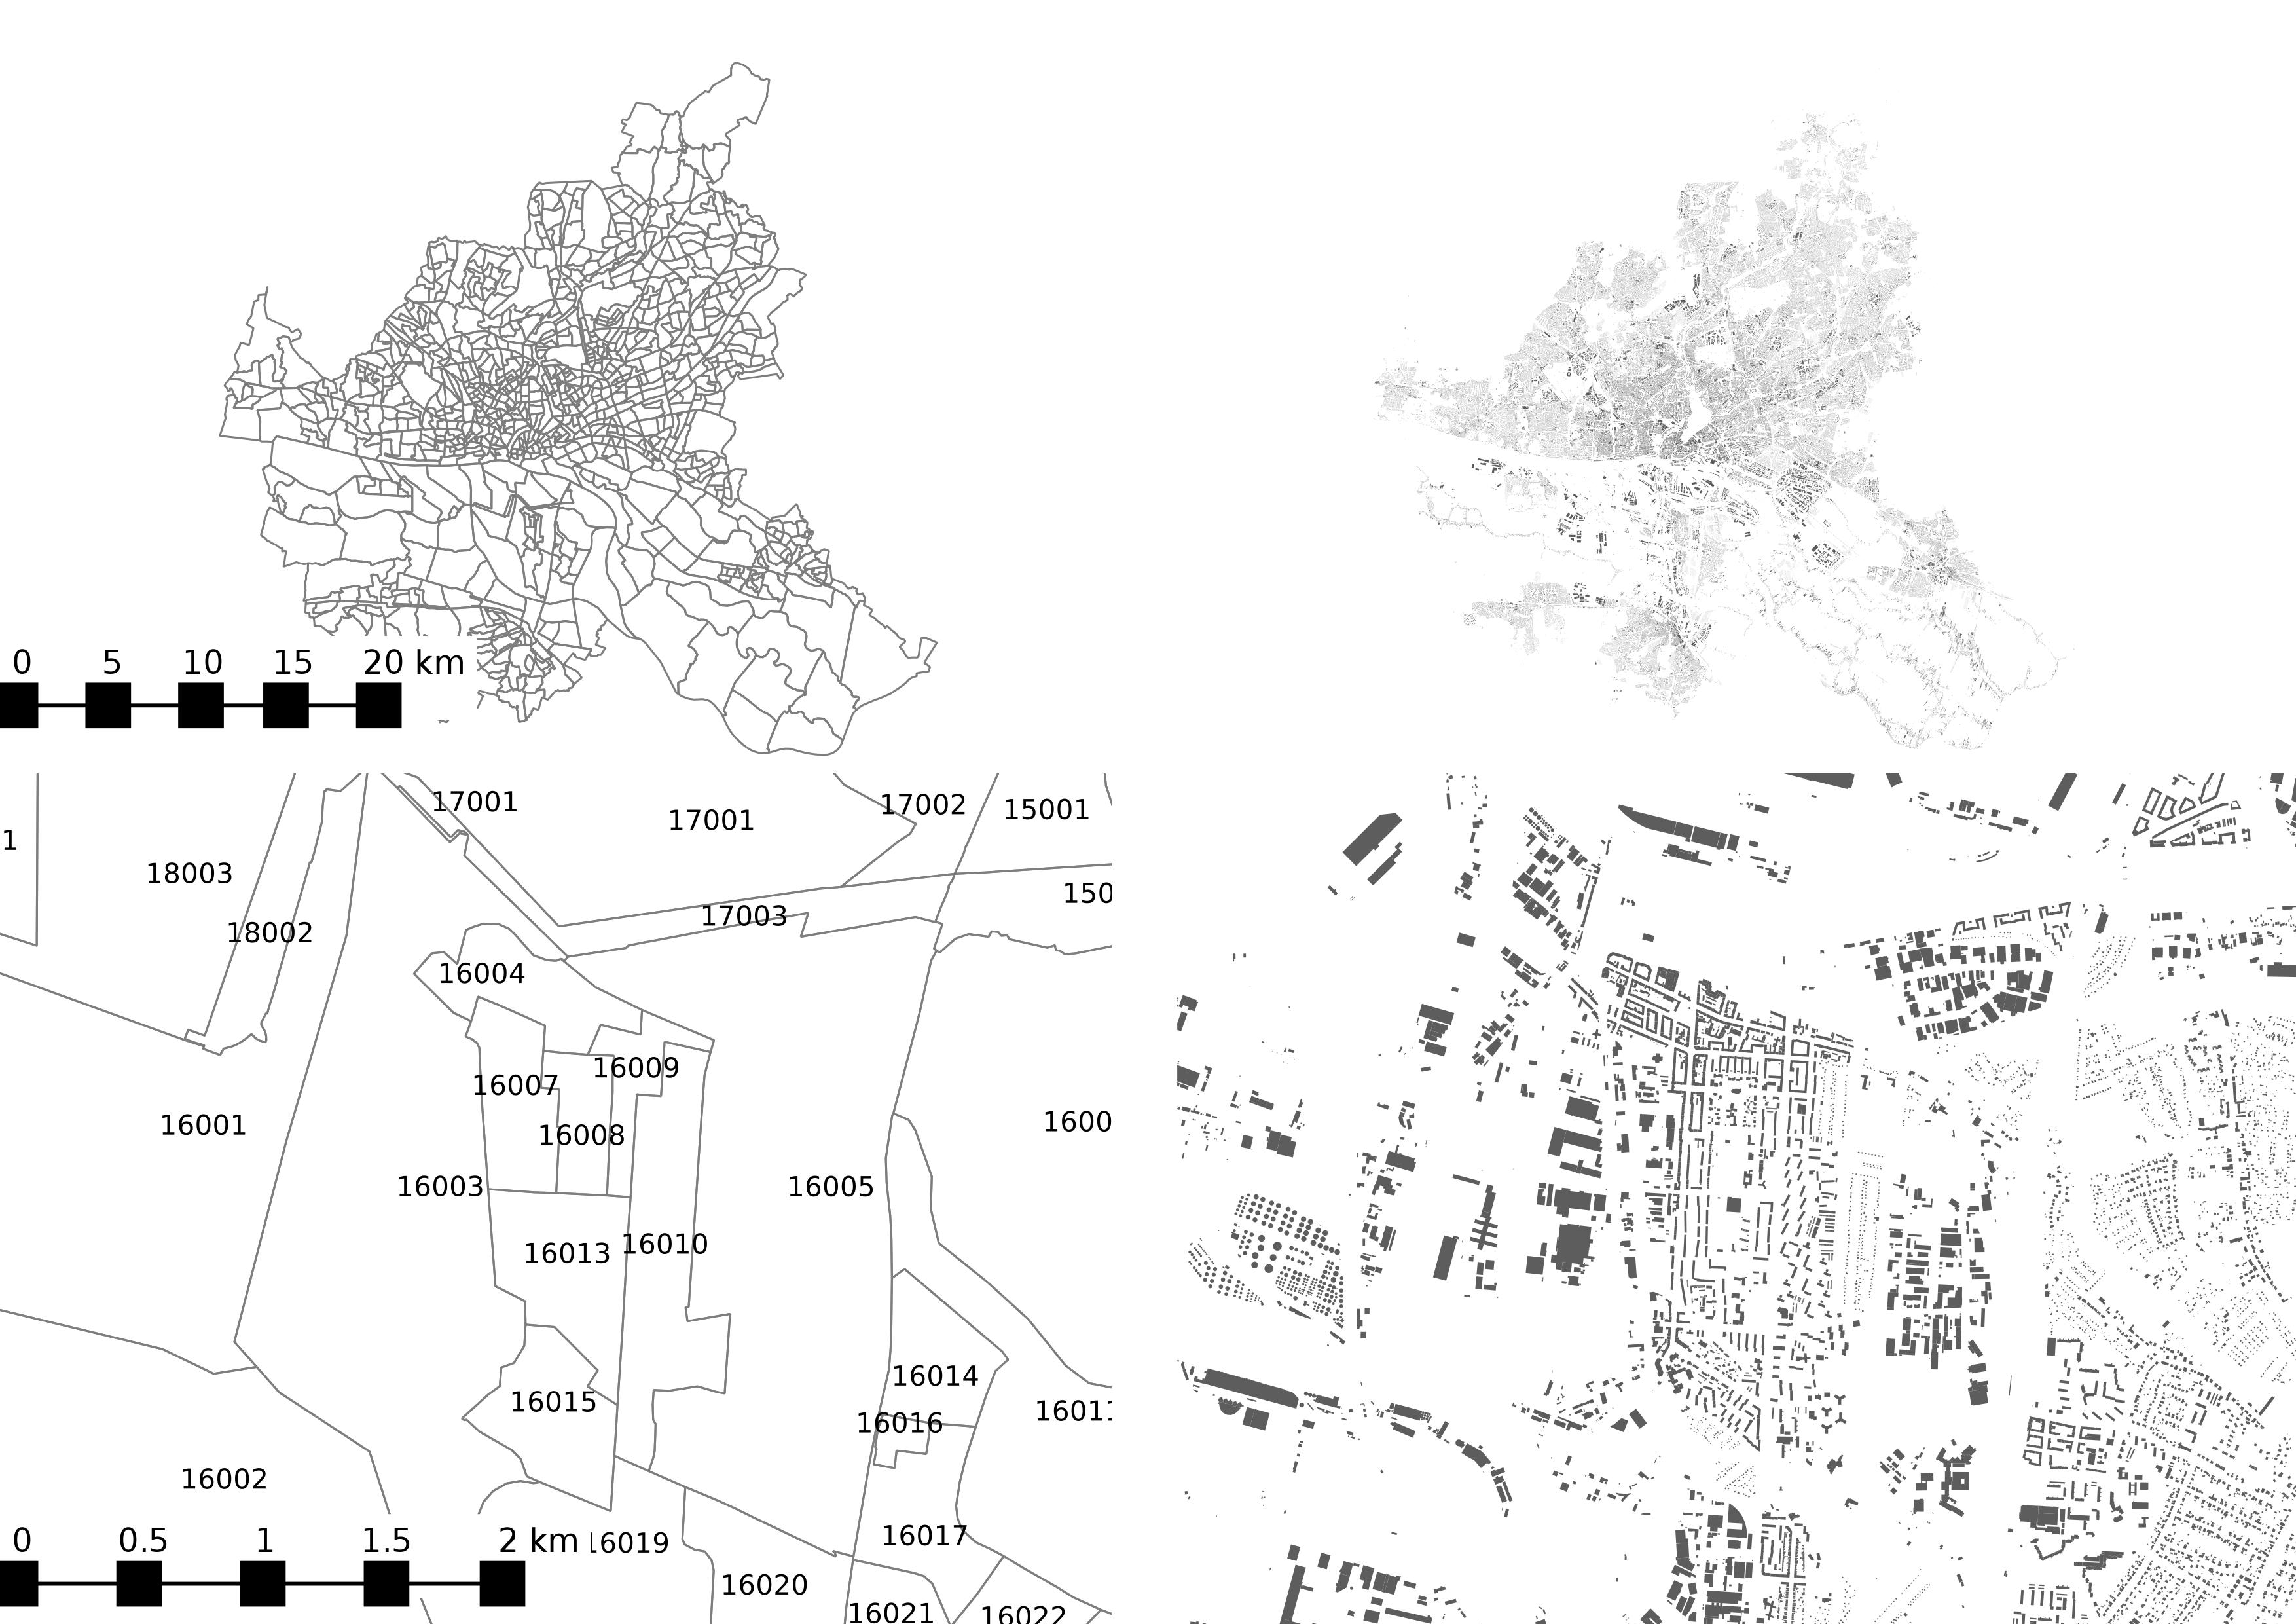
\includegraphics[width=\textwidth]{FIGURES/Data.jpg}
    \begin{flushleft}
    \begin{footnotesize}
(a) Statistical areas ``Statistische Gebiete'' containing aggregated
sociodemographic information. Statistisches Amt für Hamburg und
Schleswig-Holstein (StaNord); and (b) Digital cadaster ALKIS ``Amtliches
Liegenschaftskatasterinformationssystem''. \citeA{ALKIS}
    \end{footnotesize}
    \end{flushleft}
\end{figure}

\section{Computing heat demand vs.\ simulating heat consumption: state of the
art in urban heat modelling, and our contribution }
\label{sec:4}

Assessing the heat use of buildings can essentially be achieved by two methods,
which exist in different variations. Simply speaking, heat demand is computed
by constructing a static heat flow balance (or heat accounting balance). German
regulations for building energy efficiency employ this approach and define a
legally binding procedure, along with parameter values on the occupant, to
implement the regulation. See DIN V 18599  \citeA{DIN.2011}.  By contrast,
there is also dynamic thermal simulation, taking account of spatial-temporal
heat flows in the building and detailed circumstances, including occupant
characteristics. The latter is the most common method used in the building
simulation community \citeA{Hensen.2011} which is dominated by physicists and
engineers.

Thus, \textit{demand} usually means a hypothetical figure computed in a static
energy balance from energy-relevant properties of the building, assuming a
normal occupant. \textit{Consumption}, on the other hand, is what a building
actually consumes --- a real or a simulated figure that reflects real world
deviations from the norm, caused by, for example, occupant attributes and
behaviour that deviates from the norm. One could distinguish a third specimen
of model used by economists and social scientists, a statistical approach,
relating energy consumption to building occupants (or building characteristics)
based on observed consumption data, without explicitly accounting for heat
flows.

Our ultimate objective is to simulate heat consumption. For this model,
therefore, we take a simple approach, using a static heat accounting tool which
traditionally is used to assess heat demand, in which we vary the assumptions
based on the occupants of the building, such as interior heat gains, air flow,
and desired indoor temperature.

Other attempts to perform a simulation of energy consumption at an urban scale
using micro units have been performed by \citeA{Haldi.2011, Chingcuanco.2012,
Jackson.2008}.  \citeauthor{Haldi.2011} develop their own urban energy demand
model (CitySim), which implements a simple thermal simulation, accounting for
varying occupants (for more detail see \citeA{Robinson.2011, Page.2008,
Page.2007}), describing the occupants' presence model which is central to our
own approach. The model can be extended to simulate entire urban areas.  The
authors make use of a Markov-Chain model for generating occupancy rates, thus
representing a possible spread of heat demand patterns at an urban scale.  It
is our aim to expand these approaches, applying the concept of spatial
microsimulation to connect demographic characteristics of an urban area,
allowing us to observe specific spread patterns of heat demand of the
corresponding urban areas. \citeauthor{Chingcuanco.2012} attempt to combine a
simulation model (ILUTE)\footnote{Integrated Land Use, Transportation,
Environment modelling system.} working at a micro level with an energy balance
model developed specifically for the region under analysis. The first
simulation model delivers much of the required data for the heat accounting
model.

\begin{figure}[htb]
    \caption{Occupant influence on different building typologies arrange by
    	construction year}\label{fig:3} 
    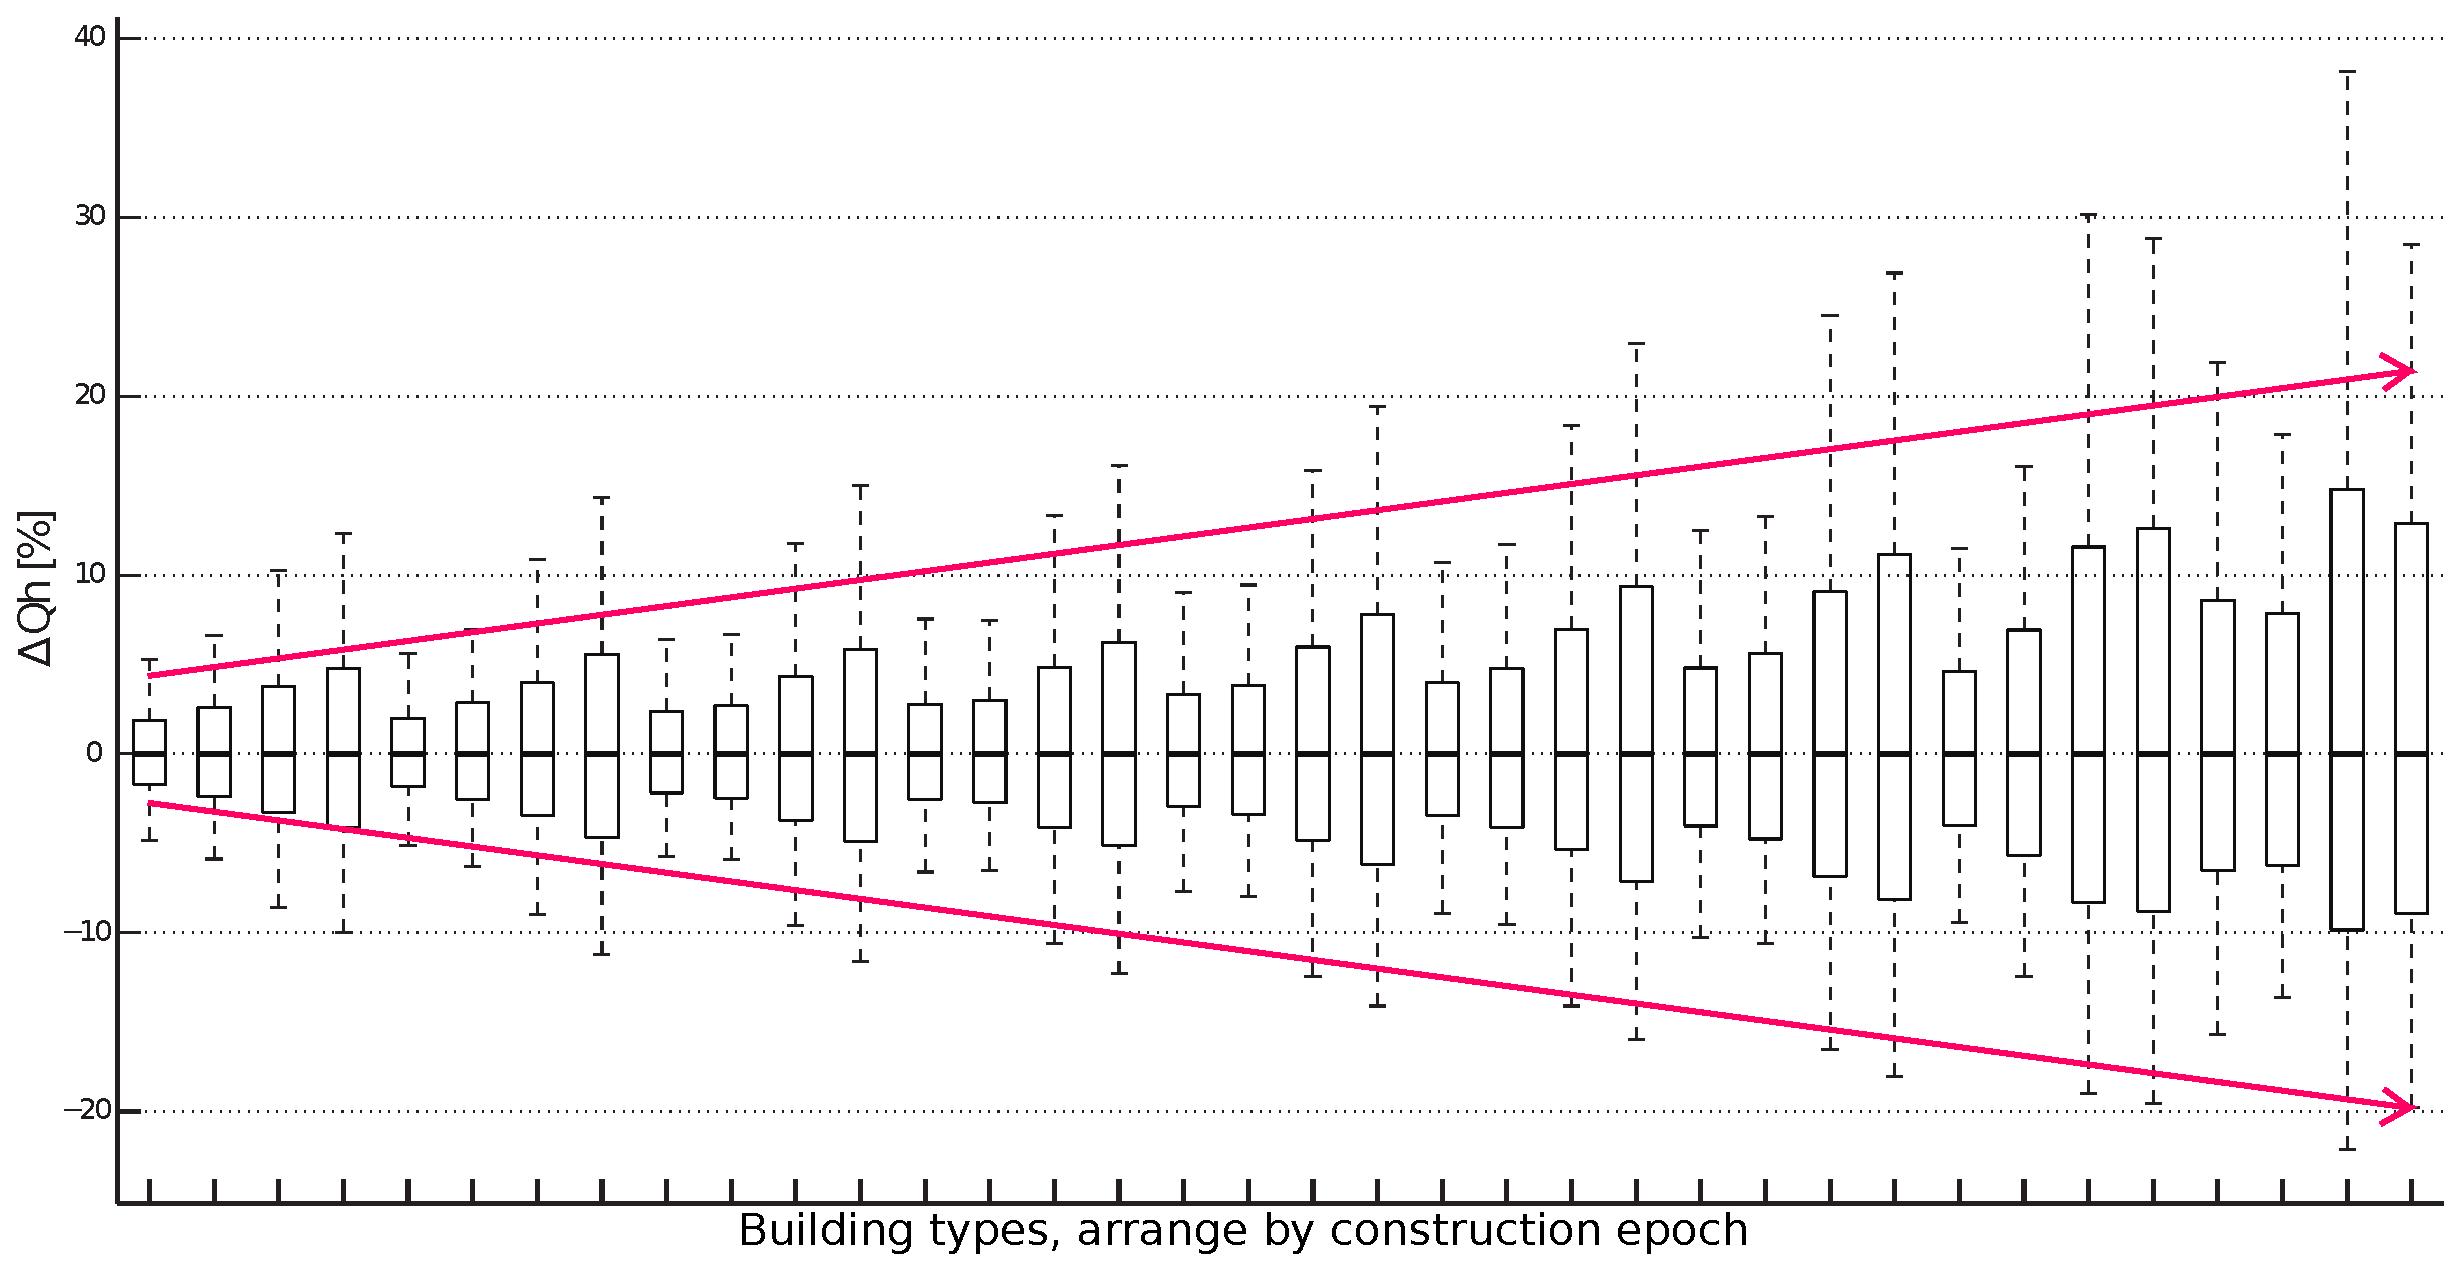
\includegraphics[width=\linewidth]{FIGURES/Typ_different_dim_percentage_line.eps}
\end{figure}

The study of the influence of occupant characteristics and occupant behaviour
on energy demand has a long tradition in economics \citeA{Scott.1980,
vanRaaij.1982, vanRaaij.1983b, Bohi.1984}. A general problem of these
studies is the level of aggregation in the data which records energy
consumption across a group of consumers with different characteristics, often
not in panel-data format, and often fails to control for the quality of the
building (because that data has not been available).

The integration of the occupant influence on various types of dynamic thermal
building simulation models has also been studied by others. Almost all the
scientific work in this field has been performed at a building level. The area
of building simulation addresses this topic in a marginal fashion
\citeA{Mahdavi.2011}. It is essential for the further development of heat
supply infrastructure in urban environments that a clear understanding of heat
consumption patterns at a low level of aggregation is achieved.

A clear difficulty with empirical observations of occupant behaviour
influencing energy demand is the need to control for all relevant factors
\citeA{Yu.2011}. An important factor for the simulation of energy demand seems
to be occupant presence \citeA{GuerraSantin.2009}, the latter authors observing
this effect in their work, \citeA{Page.2008} developed an interesting method
for the integration of this parameter into simulation models.  The authors
simulate a time series of occupantsr' presence using a stochastic model.
\citeA{Widen.2011} make an interesting contribution on the use of time-use data
for the modeling of occupant influence in the residential sector. Further
methods to integrate occupant behaviour into energy simulation models have been
developed \citeA{Borgeson.2008, Hoes.2009, Hensen.2011, Ludemann.2001,
Nouidui.2012} Table~\ref{tab:1} is a rough cut at the literature, classifying
modelling approaches reported there and illustrating where our approach is
placed.

Returning to our approach which uses a static balancing tool to compute heat
demand, but varying parameters that may be influenced by the occupants:
Figure~\ref{fig:3} shows occupant influence on 36 buildings.  We calculated the
heat demand for each of these buildings varying ``occupant parameters''. The
variation representing occupant behaviour is performed by the combination of
three key input variables: (1) $q_i[W/m^2] = $ Internal heat emissions; (2)
$T_i[C^\circ] = $ Internal temperature; and (3) $n[h^{-1}] = $ Air exchange
rate. In the plot the buildings are arranged by construction period (from
oldest to newest). We vary the quality of the building shell along with the
construction period. Newer buildings have a better insulated shell. It is clear
that the influence of occupant behaviour (measured as relative heat variation
$\Delta Qh$ in percent) is highest on newer buildings.

This literature shows that the integration of occupant behaviour into building
simulation models can be achieved. Difficulties arise with the validation of
such simulations, as empirical data at the needed temporal and disaggregation
resolution is still very hard to get.

\begin{table}[htb] 
    \caption{Different types of models for energy simulation of
    buildings}\label{tab:1} \centering
    \begin{tabular}{p{4.5cm}|*{3}{p{3.2cm}}}
        \toprule 
        \multicolumn{1}{r|}{Model type} & 
        static heat balance model (at individual building level)& 
        dynamic thermal simulation model (at individual building level)& 
        statistical model relating heat consumption to occupants, at
        various levels of aggregation, no heat balance imposed\\ 
        Occupant Type \\
        \midrule
        ``Average Occupant'' (household comprised of identical norm persons; only
        their number counts)& 
        \cite{Blesl.2007, DIN.2011, 
        Dascalaki.2011, Loga.2011}&
        \cite{EnergyPlusDevelopmentTeam.2012, Hensen.2011} \\ 
        \midrule
        Household with individualized demographics and behaviour&
        \cite{Chingcuanco.2012, Munoz.2013b} &
        \cite{Ludemann.2001, Borgeson.2008, Page.2008,
        Mahdavi.2011, Widen.2011} & \cite{Scott.1980, Bohi.1984,
        GuerraSantin.2009} \\ 
        \bottomrule
    \end{tabular} 
\end{table}

\section{constructing synthetic populations for statistical areas}
\label{sec:5}

The selected households for the specific ``statistical areas'' come from the
official German Microcensus (see Section~\ref{sec:3}).

We select entire households from the Microcensus data base set and fit them
(with an algorithm described below) into a statistical area such that the
aggregated sociodemographic data of this area are matched. We are interested in
households rather than individuals, as in the next step we will allocate these
households into dwelling units.

Table~\ref{tab:2} shows the six variables that we use to fit the households
into the statistical areas. Of these six variables, two are taken directly from
the Microcensus, and four we computed based upon other variables of the census.
We use a combinatorial optimization, Hill Climbing (HC), algorithm to fit
households from the micro census into statistical areas, following the method
presented by \citeA{Williamson.1998, Harland.2012} The TAE is calculated, for
each statistical area, by forming a weighted sum of the absolute errors of the
household variables of Table~\ref{tab:2}. See Equation~\ref{eq:1} for the
computation of the TAE and Equation~\ref{eq:2} for the computation of the
weights. Referring to Table~\ref{tab:2}, the variable ef455 has nine possible
values (corresponding to 9 construction periods), and Variable ef451 has four
possible values (corresponding to 4 classes of numbers of dwelling units in the
building the individual lives in).

\begin{table}[htb]
    \centering
    \caption{Variables used to fit households from the Microcensus into
    statistical areas}\label{tab:2}
    \begin{tabular}{l l}
        \addlinespace \toprule
        \multicolumn{2}{l}{\textbf{Constructed variables} }\\ 
        \textbf{Variable ID} & \textbf{Variable Name} \\ 
        / & Average household size (No.\ of individuals per dwelling unit)\\ 
        / & Number of single households\\ 
        / & Number of households with children\\ 
        / & Number of single parent households\\ 
        \midrule \addlinespace
        \multicolumn{2}{l}{\textbf{Variables directly taken from the micro-census} }\\
        %\textbf{Variable ID} & \textbf{Variable Name} \\ 
        \textbf{ef455} & In what year was your home built?\\ 
        \textbf{ef451} & How many dwelling units has the building in which you 
            are living?\\ 
        \bottomrule 
    \end{tabular} \\
    %\begin{flushright} 
        \begin{footnotesize} 
            Source: MIKROZENSUS~2002~\cite{StatistischesBundesamt.2002}. 
            Variable names: translation by the authors.\\ 
        \end{footnotesize} 
    %\end{flushright} 
\end{table}

The errors for all variables (except ``average household size'') are computed
based on the number of families in the specific value class of that variable.
This would not make sense for the variable ``average household size''. The
error for the latter is computed differently, based on the total number of
families in the specific area.

\parbox{\textwidth}{
    \begin{equation} 
        \label{eq:1} 
        TAE_i = \sum_{k} |T_i^{k} - T_i^{k}(obs)| * W^k 
    \end{equation} 
    
    \begin{equation} 
        \label{eq:2} 
        W^k = \begin{cases} 
            NI_{i} \div HHs_{i}(Obs) \div 2 & \text{if $k$ = average size of
                household} \\ 
            1 & \text{else} 
        \end{cases} 
    \end{equation} 

    \noindent Where:\\
    \begin{tabular}{lp{15cm}} 
        $TAE_i$ & Total Absolute Error of statistical area $i$ \\ 
        $T_i^{k}$ & Estimated variable $k$ for statistical area $i$, 
            where $k = 1, \dots , 6$ \\ 
        $T_i^{k}(obs)$ & Observed variable $k$ for statistical area $i$ \\ 
        $W_i^k$ & Weight factor of variable $k$ for statistical area $i$\\
        $NI_{i}$ & Observed number of individuals for statistical area $i$ \\
        $HHs_{i}(Obs)$ & Observed average household size for statistical 
            area $i$ \\
    \end{tabular} 
}


The variable ``average household size'' receives a smaller weight than the other
variables because otherwise it would exert an inappropriate influence on the
fitting process. The division by 2 is an ad hoc choice that seems to smooth
the computation process well.

\begin{figure}[htb]
    \caption{Performance of the algorithm used for selecting households to fit
    aggregate values of statistical area 16004}\label{fig:4}
    \centering 
    % Created by tikzDevice version 0.6.2-92-0ad2792 on 2013-11-26 22:57:19
% !TEX encoding = UTF-8 Unicode
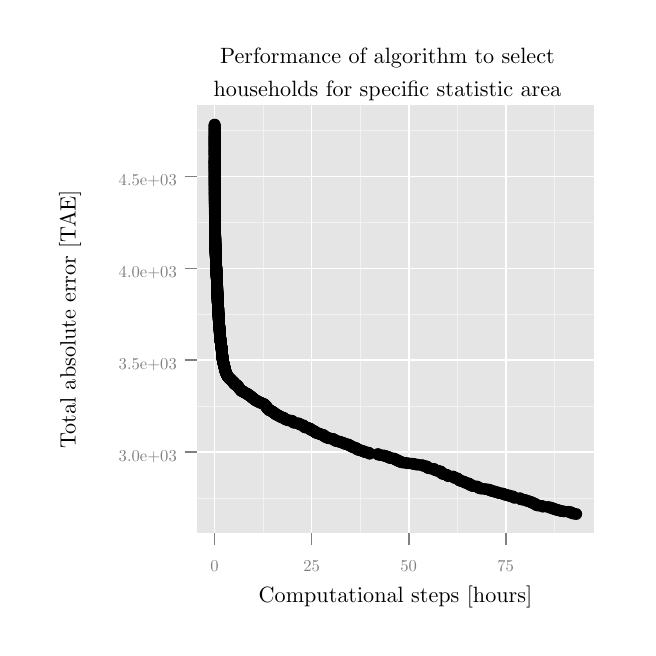
\begin{tikzpicture}[x=1pt,y=1pt]
\definecolor[named]{fillColor}{rgb}{1.00,1.00,1.00}
\path[use as bounding box,fill=fillColor,fill opacity=0.00] (0,0) rectangle (216.81,216.81);
\begin{scope}
\path[clip] (  0.00,  0.00) rectangle (216.81,216.81);
\definecolor[named]{drawColor}{rgb}{1.00,1.00,1.00}
\definecolor[named]{fillColor}{rgb}{1.00,1.00,1.00}

\path[draw=drawColor,line width= 0.6pt,line join=round,line cap=round,fill=fillColor] ( -0.00,  0.00) rectangle (216.81,216.81);
\end{scope}
\begin{scope}
\path[clip] ( 61.01, 34.03) rectangle (204.77,188.82);
\definecolor[named]{fillColor}{rgb}{0.90,0.90,0.90}

\path[fill=fillColor] ( 61.01, 34.03) rectangle (204.76,188.82);
\definecolor[named]{drawColor}{rgb}{0.95,0.95,0.95}

\path[draw=drawColor,line width= 0.3pt,line join=round] ( 61.01, 46.78) --
	(204.77, 46.78);

\path[draw=drawColor,line width= 0.3pt,line join=round] ( 61.01, 80.00) --
	(204.77, 80.00);

\path[draw=drawColor,line width= 0.3pt,line join=round] ( 61.01,113.22) --
	(204.77,113.22);

\path[draw=drawColor,line width= 0.3pt,line join=round] ( 61.01,146.44) --
	(204.77,146.44);

\path[draw=drawColor,line width= 0.3pt,line join=round] ( 61.01,179.66) --
	(204.77,179.66);

\path[draw=drawColor,line width= 0.3pt,line join=round] ( 85.08, 34.03) --
	( 85.08,188.82);

\path[draw=drawColor,line width= 0.3pt,line join=round] (120.14, 34.03) --
	(120.14,188.82);

\path[draw=drawColor,line width= 0.3pt,line join=round] (155.21, 34.03) --
	(155.21,188.82);

\path[draw=drawColor,line width= 0.3pt,line join=round] (190.27, 34.03) --
	(190.27,188.82);
\definecolor[named]{drawColor}{rgb}{1.00,1.00,1.00}

\path[draw=drawColor,line width= 0.6pt,line join=round] ( 61.01, 63.39) --
	(204.77, 63.39);

\path[draw=drawColor,line width= 0.6pt,line join=round] ( 61.01, 96.61) --
	(204.77, 96.61);

\path[draw=drawColor,line width= 0.6pt,line join=round] ( 61.01,129.83) --
	(204.77,129.83);

\path[draw=drawColor,line width= 0.6pt,line join=round] ( 61.01,163.05) --
	(204.77,163.05);

\path[draw=drawColor,line width= 0.6pt,line join=round] ( 67.55, 34.03) --
	( 67.55,188.82);

\path[draw=drawColor,line width= 0.6pt,line join=round] (102.61, 34.03) --
	(102.61,188.82);

\path[draw=drawColor,line width= 0.6pt,line join=round] (137.68, 34.03) --
	(137.68,188.82);

\path[draw=drawColor,line width= 0.6pt,line join=round] (172.74, 34.03) --
	(172.74,188.82);
\definecolor[named]{fillColor}{rgb}{0.00,0.00,0.00}

\path[fill=fillColor] ( 67.55,181.79) circle (  2.13);

\path[fill=fillColor] ( 67.55,181.66) circle (  2.13);

\path[fill=fillColor] ( 67.55,181.52) circle (  2.13);

\path[fill=fillColor] ( 67.55,181.39) circle (  2.13);

\path[fill=fillColor] ( 67.55,181.32) circle (  2.13);

\path[fill=fillColor] ( 67.55,181.19) circle (  2.13);

\path[fill=fillColor] ( 67.55,180.86) circle (  2.13);

\path[fill=fillColor] ( 67.55,180.66) circle (  2.13);

\path[fill=fillColor] ( 67.55,180.53) circle (  2.13);

\path[fill=fillColor] ( 67.55,180.39) circle (  2.13);

\path[fill=fillColor] ( 67.55,180.13) circle (  2.13);

\path[fill=fillColor] ( 67.55,180.00) circle (  2.13);

\path[fill=fillColor] ( 67.55,179.93) circle (  2.13);

\path[fill=fillColor] ( 67.55,179.80) circle (  2.13);

\path[fill=fillColor] ( 67.55,179.66) circle (  2.13);

\path[fill=fillColor] ( 67.55,179.46) circle (  2.13);

\path[fill=fillColor] ( 67.55,179.33) circle (  2.13);

\path[fill=fillColor] ( 67.55,179.13) circle (  2.13);

\path[fill=fillColor] ( 67.55,178.93) circle (  2.13);

\path[fill=fillColor] ( 67.55,178.73) circle (  2.13);

\path[fill=fillColor] ( 67.55,178.60) circle (  2.13);

\path[fill=fillColor] ( 67.55,178.47) circle (  2.13);

\path[fill=fillColor] ( 67.55,178.33) circle (  2.13);

\path[fill=fillColor] ( 67.55,178.13) circle (  2.13);

\path[fill=fillColor] ( 67.55,178.00) circle (  2.13);

\path[fill=fillColor] ( 67.55,177.80) circle (  2.13);

\path[fill=fillColor] ( 67.55,177.67) circle (  2.13);

\path[fill=fillColor] ( 67.55,177.60) circle (  2.13);

\path[fill=fillColor] ( 67.55,177.47) circle (  2.13);

\path[fill=fillColor] ( 67.55,177.27) circle (  2.13);

\path[fill=fillColor] ( 67.55,177.14) circle (  2.13);

\path[fill=fillColor] ( 67.55,177.01) circle (  2.13);

\path[fill=fillColor] ( 67.55,176.94) circle (  2.13);

\path[fill=fillColor] ( 67.55,176.87) circle (  2.13);

\path[fill=fillColor] ( 67.55,176.67) circle (  2.13);

\path[fill=fillColor] ( 67.55,176.54) circle (  2.13);

\path[fill=fillColor] ( 67.55,176.34) circle (  2.13);

\path[fill=fillColor] ( 67.55,176.21) circle (  2.13);

\path[fill=fillColor] ( 67.55,176.08) circle (  2.13);

\path[fill=fillColor] ( 67.55,175.94) circle (  2.13);

\path[fill=fillColor] ( 67.55,175.88) circle (  2.13);

\path[fill=fillColor] ( 67.55,175.81) circle (  2.13);

\path[fill=fillColor] ( 67.55,175.74) circle (  2.13);

\path[fill=fillColor] ( 67.55,175.54) circle (  2.13);

\path[fill=fillColor] ( 67.55,175.34) circle (  2.13);

\path[fill=fillColor] ( 67.55,175.15) circle (  2.13);

\path[fill=fillColor] ( 67.55,175.08) circle (  2.13);

\path[fill=fillColor] ( 67.55,175.01) circle (  2.13);

\path[fill=fillColor] ( 67.55,174.88) circle (  2.13);

\path[fill=fillColor] ( 67.55,174.75) circle (  2.13);

\path[fill=fillColor] ( 67.55,174.55) circle (  2.13);

\path[fill=fillColor] ( 67.55,174.41) circle (  2.13);

\path[fill=fillColor] ( 67.55,174.28) circle (  2.13);

\path[fill=fillColor] ( 67.55,174.15) circle (  2.13);

\path[fill=fillColor] ( 67.55,174.02) circle (  2.13);

\path[fill=fillColor] ( 67.55,173.95) circle (  2.13);

\path[fill=fillColor] ( 67.55,173.82) circle (  2.13);

\path[fill=fillColor] ( 67.55,173.62) circle (  2.13);

\path[fill=fillColor] ( 67.55,173.48) circle (  2.13);

\path[fill=fillColor] ( 67.55,173.22) circle (  2.13);

\path[fill=fillColor] ( 67.55,173.09) circle (  2.13);

\path[fill=fillColor] ( 67.55,173.02) circle (  2.13);

\path[fill=fillColor] ( 67.55,172.89) circle (  2.13);

\path[fill=fillColor] ( 67.55,172.62) circle (  2.13);

\path[fill=fillColor] ( 67.55,172.55) circle (  2.13);

\path[fill=fillColor] ( 67.55,172.42) circle (  2.13);

\path[fill=fillColor] ( 67.55,172.35) circle (  2.13);

\path[fill=fillColor] ( 67.55,172.16) circle (  2.13);

\path[fill=fillColor] ( 67.55,172.02) circle (  2.13);

\path[fill=fillColor] ( 67.55,171.89) circle (  2.13);

\path[fill=fillColor] ( 67.55,171.76) circle (  2.13);

\path[fill=fillColor] ( 67.55,171.56) circle (  2.13);

\path[fill=fillColor] ( 67.55,171.36) circle (  2.13);

\path[fill=fillColor] ( 67.55,171.29) circle (  2.13);

\path[fill=fillColor] ( 67.55,171.16) circle (  2.13);

\path[fill=fillColor] ( 67.55,171.09) circle (  2.13);

\path[fill=fillColor] ( 67.55,170.96) circle (  2.13);

\path[fill=fillColor] ( 67.55,170.83) circle (  2.13);

\path[fill=fillColor] ( 67.55,170.69) circle (  2.13);

\path[fill=fillColor] ( 67.55,170.29) circle (  2.13);

\path[fill=fillColor] ( 67.55,170.10) circle (  2.13);

\path[fill=fillColor] ( 67.55,169.96) circle (  2.13);

\path[fill=fillColor] ( 67.55,169.83) circle (  2.13);

\path[fill=fillColor] ( 67.55,169.63) circle (  2.13);

\path[fill=fillColor] ( 67.55,169.50) circle (  2.13);

\path[fill=fillColor] ( 67.55,169.23) circle (  2.13);

\path[fill=fillColor] ( 67.55,169.03) circle (  2.13);

\path[fill=fillColor] ( 67.55,168.97) circle (  2.13);

\path[fill=fillColor] ( 67.55,168.83) circle (  2.13);

\path[fill=fillColor] ( 67.55,168.77) circle (  2.13);

\path[fill=fillColor] ( 67.55,168.50) circle (  2.13);

\path[fill=fillColor] ( 67.55,168.37) circle (  2.13);

\path[fill=fillColor] ( 67.55,168.30) circle (  2.13);

\path[fill=fillColor] ( 67.55,168.24) circle (  2.13);

\path[fill=fillColor] ( 67.55,168.17) circle (  2.13);

\path[fill=fillColor] ( 67.55,168.10) circle (  2.13);

\path[fill=fillColor] ( 67.55,167.97) circle (  2.13);

\path[fill=fillColor] ( 67.56,167.90) circle (  2.13);

\path[fill=fillColor] ( 67.56,167.84) circle (  2.13);

\path[fill=fillColor] ( 67.56,167.77) circle (  2.13);

\path[fill=fillColor] ( 67.56,167.64) circle (  2.13);

\path[fill=fillColor] ( 67.56,167.57) circle (  2.13);

\path[fill=fillColor] ( 67.56,167.44) circle (  2.13);

\path[fill=fillColor] ( 67.56,167.31) circle (  2.13);

\path[fill=fillColor] ( 67.56,167.24) circle (  2.13);

\path[fill=fillColor] ( 67.56,167.11) circle (  2.13);

\path[fill=fillColor] ( 67.56,166.97) circle (  2.13);

\path[fill=fillColor] ( 67.56,166.91) circle (  2.13);

\path[fill=fillColor] ( 67.56,166.77) circle (  2.13);

\path[fill=fillColor] ( 67.56,166.71) circle (  2.13);

\path[fill=fillColor] ( 67.56,166.57) circle (  2.13);

\path[fill=fillColor] ( 67.56,166.51) circle (  2.13);

\path[fill=fillColor] ( 67.56,166.38) circle (  2.13);

\path[fill=fillColor] ( 67.56,166.31) circle (  2.13);

\path[fill=fillColor] ( 67.56,166.24) circle (  2.13);

\path[fill=fillColor] ( 67.56,166.11) circle (  2.13);

\path[fill=fillColor] ( 67.56,165.98) circle (  2.13);

\path[fill=fillColor] ( 67.56,165.91) circle (  2.13);

\path[fill=fillColor] ( 67.56,165.78) circle (  2.13);

\path[fill=fillColor] ( 67.56,165.71) circle (  2.13);

\path[fill=fillColor] ( 67.56,165.64) circle (  2.13);

\path[fill=fillColor] ( 67.56,165.51) circle (  2.13);

\path[fill=fillColor] ( 67.57,165.38) circle (  2.13);

\path[fill=fillColor] ( 67.57,165.25) circle (  2.13);

\path[fill=fillColor] ( 67.57,165.18) circle (  2.13);

\path[fill=fillColor] ( 67.57,165.11) circle (  2.13);

\path[fill=fillColor] ( 67.57,164.98) circle (  2.13);

\path[fill=fillColor] ( 67.57,164.91) circle (  2.13);

\path[fill=fillColor] ( 67.57,164.85) circle (  2.13);

\path[fill=fillColor] ( 67.57,164.78) circle (  2.13);

\path[fill=fillColor] ( 67.57,164.65) circle (  2.13);

\path[fill=fillColor] ( 67.57,164.58) circle (  2.13);

\path[fill=fillColor] ( 67.57,164.45) circle (  2.13);

\path[fill=fillColor] ( 67.57,164.38) circle (  2.13);

\path[fill=fillColor] ( 67.58,164.32) circle (  2.13);

\path[fill=fillColor] ( 67.58,164.18) circle (  2.13);

\path[fill=fillColor] ( 67.58,164.05) circle (  2.13);

\path[fill=fillColor] ( 67.58,163.92) circle (  2.13);

\path[fill=fillColor] ( 67.58,163.85) circle (  2.13);

\path[fill=fillColor] ( 67.58,163.72) circle (  2.13);

\path[fill=fillColor] ( 67.58,163.65) circle (  2.13);

\path[fill=fillColor] ( 67.58,163.52) circle (  2.13);

\path[fill=fillColor] ( 67.58,163.45) circle (  2.13);

\path[fill=fillColor] ( 67.58,163.39) circle (  2.13);

\path[fill=fillColor] ( 67.58,163.25) circle (  2.13);

\path[fill=fillColor] ( 67.58,163.19) circle (  2.13);

\path[fill=fillColor] ( 67.58,163.12) circle (  2.13);

\path[fill=fillColor] ( 67.58,163.05) circle (  2.13);

\path[fill=fillColor] ( 67.58,162.99) circle (  2.13);

\path[fill=fillColor] ( 67.58,162.92) circle (  2.13);

\path[fill=fillColor] ( 67.58,162.85) circle (  2.13);

\path[fill=fillColor] ( 67.58,162.79) circle (  2.13);

\path[fill=fillColor] ( 67.58,162.65) circle (  2.13);

\path[fill=fillColor] ( 67.58,162.52) circle (  2.13);

\path[fill=fillColor] ( 67.58,162.46) circle (  2.13);

\path[fill=fillColor] ( 67.58,162.32) circle (  2.13);

\path[fill=fillColor] ( 67.58,162.26) circle (  2.13);

\path[fill=fillColor] ( 67.58,162.19) circle (  2.13);

\path[fill=fillColor] ( 67.59,162.06) circle (  2.13);

\path[fill=fillColor] ( 67.59,161.99) circle (  2.13);

\path[fill=fillColor] ( 67.59,161.92) circle (  2.13);

\path[fill=fillColor] ( 67.59,161.86) circle (  2.13);

\path[fill=fillColor] ( 67.59,161.79) circle (  2.13);

\path[fill=fillColor] ( 67.59,161.72) circle (  2.13);

\path[fill=fillColor] ( 67.59,161.66) circle (  2.13);

\path[fill=fillColor] ( 67.59,161.52) circle (  2.13);

\path[fill=fillColor] ( 67.59,161.46) circle (  2.13);

\path[fill=fillColor] ( 67.59,161.39) circle (  2.13);

\path[fill=fillColor] ( 67.59,161.33) circle (  2.13);

\path[fill=fillColor] ( 67.59,161.26) circle (  2.13);

\path[fill=fillColor] ( 67.59,161.13) circle (  2.13);

\path[fill=fillColor] ( 67.59,161.06) circle (  2.13);

\path[fill=fillColor] ( 67.59,160.99) circle (  2.13);

\path[fill=fillColor] ( 67.59,160.93) circle (  2.13);

\path[fill=fillColor] ( 67.59,160.79) circle (  2.13);

\path[fill=fillColor] ( 67.59,160.66) circle (  2.13);

\path[fill=fillColor] ( 67.59,160.59) circle (  2.13);

\path[fill=fillColor] ( 67.59,160.46) circle (  2.13);

\path[fill=fillColor] ( 67.59,160.40) circle (  2.13);

\path[fill=fillColor] ( 67.59,160.33) circle (  2.13);

\path[fill=fillColor] ( 67.59,160.26) circle (  2.13);

\path[fill=fillColor] ( 67.59,160.20) circle (  2.13);

\path[fill=fillColor] ( 67.59,160.13) circle (  2.13);

\path[fill=fillColor] ( 67.59,160.06) circle (  2.13);

\path[fill=fillColor] ( 67.59,160.00) circle (  2.13);

\path[fill=fillColor] ( 67.59,159.86) circle (  2.13);

\path[fill=fillColor] ( 67.59,159.80) circle (  2.13);

\path[fill=fillColor] ( 67.59,159.73) circle (  2.13);

\path[fill=fillColor] ( 67.59,159.60) circle (  2.13);

\path[fill=fillColor] ( 67.60,159.47) circle (  2.13);

\path[fill=fillColor] ( 67.60,159.40) circle (  2.13);

\path[fill=fillColor] ( 67.60,159.33) circle (  2.13);

\path[fill=fillColor] ( 67.60,159.20) circle (  2.13);

\path[fill=fillColor] ( 67.60,159.13) circle (  2.13);

\path[fill=fillColor] ( 67.60,159.00) circle (  2.13);

\path[fill=fillColor] ( 67.60,158.93) circle (  2.13);

\path[fill=fillColor] ( 67.60,158.80) circle (  2.13);

\path[fill=fillColor] ( 67.60,158.73) circle (  2.13);

\path[fill=fillColor] ( 67.60,158.67) circle (  2.13);

\path[fill=fillColor] ( 67.60,158.54) circle (  2.13);

\path[fill=fillColor] ( 67.60,158.47) circle (  2.13);

\path[fill=fillColor] ( 67.60,158.40) circle (  2.13);

\path[fill=fillColor] ( 67.60,158.27) circle (  2.13);

\path[fill=fillColor] ( 67.60,158.20) circle (  2.13);

\path[fill=fillColor] ( 67.60,158.14) circle (  2.13);

\path[fill=fillColor] ( 67.60,158.07) circle (  2.13);

\path[fill=fillColor] ( 67.60,157.94) circle (  2.13);

\path[fill=fillColor] ( 67.60,157.80) circle (  2.13);

\path[fill=fillColor] ( 67.60,157.67) circle (  2.13);

\path[fill=fillColor] ( 67.60,157.54) circle (  2.13);

\path[fill=fillColor] ( 67.60,157.47) circle (  2.13);

\path[fill=fillColor] ( 67.61,157.41) circle (  2.13);

\path[fill=fillColor] ( 67.61,157.34) circle (  2.13);

\path[fill=fillColor] ( 67.61,157.27) circle (  2.13);

\path[fill=fillColor] ( 67.61,157.14) circle (  2.13);

\path[fill=fillColor] ( 67.61,157.07) circle (  2.13);

\path[fill=fillColor] ( 67.61,157.01) circle (  2.13);

\path[fill=fillColor] ( 67.61,156.94) circle (  2.13);

\path[fill=fillColor] ( 67.61,156.87) circle (  2.13);

\path[fill=fillColor] ( 67.61,156.81) circle (  2.13);

\path[fill=fillColor] ( 67.61,156.74) circle (  2.13);

\path[fill=fillColor] ( 67.61,156.67) circle (  2.13);

\path[fill=fillColor] ( 67.61,156.61) circle (  2.13);

\path[fill=fillColor] ( 67.61,156.48) circle (  2.13);

\path[fill=fillColor] ( 67.61,156.41) circle (  2.13);

\path[fill=fillColor] ( 67.61,156.28) circle (  2.13);

\path[fill=fillColor] ( 67.62,156.21) circle (  2.13);

\path[fill=fillColor] ( 67.62,156.14) circle (  2.13);

\path[fill=fillColor] ( 67.62,156.08) circle (  2.13);

\path[fill=fillColor] ( 67.62,156.01) circle (  2.13);

\path[fill=fillColor] ( 67.62,155.94) circle (  2.13);

\path[fill=fillColor] ( 67.62,155.88) circle (  2.13);

\path[fill=fillColor] ( 67.62,155.74) circle (  2.13);

\path[fill=fillColor] ( 67.62,155.68) circle (  2.13);

\path[fill=fillColor] ( 67.62,155.55) circle (  2.13);

\path[fill=fillColor] ( 67.62,155.48) circle (  2.13);

\path[fill=fillColor] ( 67.62,155.41) circle (  2.13);

\path[fill=fillColor] ( 67.62,155.28) circle (  2.13);

\path[fill=fillColor] ( 67.62,155.21) circle (  2.13);

\path[fill=fillColor] ( 67.62,155.15) circle (  2.13);

\path[fill=fillColor] ( 67.62,155.08) circle (  2.13);

\path[fill=fillColor] ( 67.62,154.95) circle (  2.13);

\path[fill=fillColor] ( 67.62,154.88) circle (  2.13);

\path[fill=fillColor] ( 67.62,154.75) circle (  2.13);

\path[fill=fillColor] ( 67.62,154.68) circle (  2.13);

\path[fill=fillColor] ( 67.62,154.55) circle (  2.13);

\path[fill=fillColor] ( 67.62,154.48) circle (  2.13);

\path[fill=fillColor] ( 67.62,154.42) circle (  2.13);

\path[fill=fillColor] ( 67.62,154.35) circle (  2.13);

\path[fill=fillColor] ( 67.62,154.22) circle (  2.13);

\path[fill=fillColor] ( 67.63,154.15) circle (  2.13);

\path[fill=fillColor] ( 67.63,154.08) circle (  2.13);

\path[fill=fillColor] ( 67.63,153.95) circle (  2.13);

\path[fill=fillColor] ( 67.63,153.82) circle (  2.13);

\path[fill=fillColor] ( 67.63,153.75) circle (  2.13);

\path[fill=fillColor] ( 67.63,153.69) circle (  2.13);

\path[fill=fillColor] ( 67.63,153.62) circle (  2.13);

\path[fill=fillColor] ( 67.63,153.55) circle (  2.13);

\path[fill=fillColor] ( 67.63,153.49) circle (  2.13);

\path[fill=fillColor] ( 67.63,153.35) circle (  2.13);

\path[fill=fillColor] ( 67.63,153.29) circle (  2.13);

\path[fill=fillColor] ( 67.64,153.22) circle (  2.13);

\path[fill=fillColor] ( 67.64,153.15) circle (  2.13);

\path[fill=fillColor] ( 67.64,153.09) circle (  2.13);

\path[fill=fillColor] ( 67.64,153.02) circle (  2.13);

\path[fill=fillColor] ( 67.64,152.89) circle (  2.13);

\path[fill=fillColor] ( 67.64,152.82) circle (  2.13);

\path[fill=fillColor] ( 67.64,152.69) circle (  2.13);

\path[fill=fillColor] ( 67.64,152.56) circle (  2.13);

\path[fill=fillColor] ( 67.64,152.49) circle (  2.13);

\path[fill=fillColor] ( 67.64,152.42) circle (  2.13);

\path[fill=fillColor] ( 67.64,152.36) circle (  2.13);

\path[fill=fillColor] ( 67.64,152.22) circle (  2.13);

\path[fill=fillColor] ( 67.64,152.16) circle (  2.13);

\path[fill=fillColor] ( 67.64,152.09) circle (  2.13);

\path[fill=fillColor] ( 67.64,152.02) circle (  2.13);

\path[fill=fillColor] ( 67.64,151.89) circle (  2.13);

\path[fill=fillColor] ( 67.64,151.76) circle (  2.13);

\path[fill=fillColor] ( 67.64,151.69) circle (  2.13);

\path[fill=fillColor] ( 67.65,151.63) circle (  2.13);

\path[fill=fillColor] ( 67.65,151.49) circle (  2.13);

\path[fill=fillColor] ( 67.65,151.36) circle (  2.13);

\path[fill=fillColor] ( 67.65,151.23) circle (  2.13);

\path[fill=fillColor] ( 67.65,151.16) circle (  2.13);

\path[fill=fillColor] ( 67.65,151.09) circle (  2.13);

\path[fill=fillColor] ( 67.65,151.03) circle (  2.13);

\path[fill=fillColor] ( 67.65,150.89) circle (  2.13);

\path[fill=fillColor] ( 67.65,150.83) circle (  2.13);

\path[fill=fillColor] ( 67.65,150.76) circle (  2.13);

\path[fill=fillColor] ( 67.65,150.70) circle (  2.13);

\path[fill=fillColor] ( 67.65,150.63) circle (  2.13);

\path[fill=fillColor] ( 67.65,150.56) circle (  2.13);

\path[fill=fillColor] ( 67.65,150.43) circle (  2.13);

\path[fill=fillColor] ( 67.65,150.30) circle (  2.13);

\path[fill=fillColor] ( 67.65,150.23) circle (  2.13);

\path[fill=fillColor] ( 67.65,150.16) circle (  2.13);

\path[fill=fillColor] ( 67.65,150.03) circle (  2.13);

\path[fill=fillColor] ( 67.65,149.96) circle (  2.13);

\path[fill=fillColor] ( 67.65,149.83) circle (  2.13);

\path[fill=fillColor] ( 67.65,149.77) circle (  2.13);

\path[fill=fillColor] ( 67.65,149.63) circle (  2.13);

\path[fill=fillColor] ( 67.65,149.50) circle (  2.13);

\path[fill=fillColor] ( 67.65,149.43) circle (  2.13);

\path[fill=fillColor] ( 67.65,149.30) circle (  2.13);

\path[fill=fillColor] ( 67.66,149.17) circle (  2.13);

\path[fill=fillColor] ( 67.66,149.10) circle (  2.13);

\path[fill=fillColor] ( 67.66,149.03) circle (  2.13);

\path[fill=fillColor] ( 67.66,148.97) circle (  2.13);

\path[fill=fillColor] ( 67.66,148.90) circle (  2.13);

\path[fill=fillColor] ( 67.66,148.84) circle (  2.13);

\path[fill=fillColor] ( 67.66,148.77) circle (  2.13);

\path[fill=fillColor] ( 67.66,148.70) circle (  2.13);

\path[fill=fillColor] ( 67.66,148.64) circle (  2.13);

\path[fill=fillColor] ( 67.66,148.57) circle (  2.13);

\path[fill=fillColor] ( 67.66,148.44) circle (  2.13);

\path[fill=fillColor] ( 67.66,148.30) circle (  2.13);

\path[fill=fillColor] ( 67.66,148.24) circle (  2.13);

\path[fill=fillColor] ( 67.66,148.17) circle (  2.13);

\path[fill=fillColor] ( 67.66,148.04) circle (  2.13);

\path[fill=fillColor] ( 67.66,147.90) circle (  2.13);

\path[fill=fillColor] ( 67.66,147.77) circle (  2.13);

\path[fill=fillColor] ( 67.66,147.64) circle (  2.13);

\path[fill=fillColor] ( 67.66,147.57) circle (  2.13);

\path[fill=fillColor] ( 67.67,147.44) circle (  2.13);

\path[fill=fillColor] ( 67.67,147.37) circle (  2.13);

\path[fill=fillColor] ( 67.67,147.31) circle (  2.13);

\path[fill=fillColor] ( 67.67,147.24) circle (  2.13);

\path[fill=fillColor] ( 67.67,147.17) circle (  2.13);

\path[fill=fillColor] ( 67.67,147.11) circle (  2.13);

\path[fill=fillColor] ( 67.67,146.97) circle (  2.13);

\path[fill=fillColor] ( 67.67,146.84) circle (  2.13);

\path[fill=fillColor] ( 67.67,146.78) circle (  2.13);

\path[fill=fillColor] ( 67.67,146.64) circle (  2.13);

\path[fill=fillColor] ( 67.67,146.58) circle (  2.13);

\path[fill=fillColor] ( 67.67,146.51) circle (  2.13);

\path[fill=fillColor] ( 67.67,146.44) circle (  2.13);

\path[fill=fillColor] ( 67.68,146.38) circle (  2.13);

\path[fill=fillColor] ( 67.68,146.24) circle (  2.13);

\path[fill=fillColor] ( 67.68,146.11) circle (  2.13);

\path[fill=fillColor] ( 67.68,145.98) circle (  2.13);

\path[fill=fillColor] ( 67.68,145.85) circle (  2.13);

\path[fill=fillColor] ( 67.68,145.71) circle (  2.13);

\path[fill=fillColor] ( 67.68,145.65) circle (  2.13);

\path[fill=fillColor] ( 67.68,145.58) circle (  2.13);

\path[fill=fillColor] ( 67.68,145.45) circle (  2.13);

\path[fill=fillColor] ( 67.68,145.31) circle (  2.13);

\path[fill=fillColor] ( 67.68,145.18) circle (  2.13);

\path[fill=fillColor] ( 67.68,145.05) circle (  2.13);

\path[fill=fillColor] ( 67.68,144.98) circle (  2.13);

\path[fill=fillColor] ( 67.69,144.85) circle (  2.13);

\path[fill=fillColor] ( 67.69,144.78) circle (  2.13);

\path[fill=fillColor] ( 67.69,144.72) circle (  2.13);

\path[fill=fillColor] ( 67.69,144.65) circle (  2.13);

\path[fill=fillColor] ( 67.69,144.58) circle (  2.13);

\path[fill=fillColor] ( 67.69,144.45) circle (  2.13);

\path[fill=fillColor] ( 67.69,144.38) circle (  2.13);

\path[fill=fillColor] ( 67.69,144.32) circle (  2.13);

\path[fill=fillColor] ( 67.69,144.25) circle (  2.13);

\path[fill=fillColor] ( 67.69,144.18) circle (  2.13);

\path[fill=fillColor] ( 67.69,144.05) circle (  2.13);

\path[fill=fillColor] ( 67.69,143.99) circle (  2.13);

\path[fill=fillColor] ( 67.69,143.85) circle (  2.13);

\path[fill=fillColor] ( 67.69,143.79) circle (  2.13);

\path[fill=fillColor] ( 67.69,143.65) circle (  2.13);

\path[fill=fillColor] ( 67.69,143.59) circle (  2.13);

\path[fill=fillColor] ( 67.69,143.45) circle (  2.13);

\path[fill=fillColor] ( 67.69,143.39) circle (  2.13);

\path[fill=fillColor] ( 67.70,143.32) circle (  2.13);

\path[fill=fillColor] ( 67.70,143.25) circle (  2.13);

\path[fill=fillColor] ( 67.70,143.19) circle (  2.13);

\path[fill=fillColor] ( 67.70,143.12) circle (  2.13);

\path[fill=fillColor] ( 67.70,143.05) circle (  2.13);

\path[fill=fillColor] ( 67.70,142.99) circle (  2.13);

\path[fill=fillColor] ( 67.70,142.86) circle (  2.13);

\path[fill=fillColor] ( 67.70,142.79) circle (  2.13);

\path[fill=fillColor] ( 67.70,142.72) circle (  2.13);

\path[fill=fillColor] ( 67.71,142.66) circle (  2.13);

\path[fill=fillColor] ( 67.71,142.59) circle (  2.13);

\path[fill=fillColor] ( 67.71,142.52) circle (  2.13);

\path[fill=fillColor] ( 67.71,142.46) circle (  2.13);

\path[fill=fillColor] ( 67.71,142.39) circle (  2.13);

\path[fill=fillColor] ( 67.72,142.32) circle (  2.13);

\path[fill=fillColor] ( 67.72,142.26) circle (  2.13);

\path[fill=fillColor] ( 67.72,142.19) circle (  2.13);

\path[fill=fillColor] ( 67.72,142.12) circle (  2.13);

\path[fill=fillColor] ( 67.73,142.06) circle (  2.13);

\path[fill=fillColor] ( 67.73,141.99) circle (  2.13);

\path[fill=fillColor] ( 67.73,141.93) circle (  2.13);

\path[fill=fillColor] ( 67.73,141.86) circle (  2.13);

\path[fill=fillColor] ( 67.73,141.79) circle (  2.13);

\path[fill=fillColor] ( 67.74,141.73) circle (  2.13);

\path[fill=fillColor] ( 67.74,141.66) circle (  2.13);

\path[fill=fillColor] ( 67.74,141.59) circle (  2.13);

\path[fill=fillColor] ( 67.74,141.46) circle (  2.13);

\path[fill=fillColor] ( 67.74,141.39) circle (  2.13);

\path[fill=fillColor] ( 67.75,141.33) circle (  2.13);

\path[fill=fillColor] ( 67.75,141.26) circle (  2.13);

\path[fill=fillColor] ( 67.75,141.19) circle (  2.13);

\path[fill=fillColor] ( 67.75,141.13) circle (  2.13);

\path[fill=fillColor] ( 67.75,141.06) circle (  2.13);

\path[fill=fillColor] ( 67.75,141.00) circle (  2.13);

\path[fill=fillColor] ( 67.76,140.93) circle (  2.13);

\path[fill=fillColor] ( 67.76,140.86) circle (  2.13);

\path[fill=fillColor] ( 67.76,140.80) circle (  2.13);

\path[fill=fillColor] ( 67.76,140.73) circle (  2.13);

\path[fill=fillColor] ( 67.76,140.66) circle (  2.13);

\path[fill=fillColor] ( 67.77,140.60) circle (  2.13);

\path[fill=fillColor] ( 67.77,140.53) circle (  2.13);

\path[fill=fillColor] ( 67.78,140.46) circle (  2.13);

\path[fill=fillColor] ( 67.78,140.40) circle (  2.13);

\path[fill=fillColor] ( 67.78,140.33) circle (  2.13);

\path[fill=fillColor] ( 67.79,140.26) circle (  2.13);

\path[fill=fillColor] ( 67.79,140.20) circle (  2.13);

\path[fill=fillColor] ( 67.79,140.13) circle (  2.13);

\path[fill=fillColor] ( 67.79,140.07) circle (  2.13);

\path[fill=fillColor] ( 67.79,140.00) circle (  2.13);

\path[fill=fillColor] ( 67.79,139.93) circle (  2.13);

\path[fill=fillColor] ( 67.80,139.87) circle (  2.13);

\path[fill=fillColor] ( 67.80,139.80) circle (  2.13);

\path[fill=fillColor] ( 67.80,139.73) circle (  2.13);

\path[fill=fillColor] ( 67.80,139.67) circle (  2.13);

\path[fill=fillColor] ( 67.80,139.60) circle (  2.13);

\path[fill=fillColor] ( 67.80,139.53) circle (  2.13);

\path[fill=fillColor] ( 67.81,139.47) circle (  2.13);

\path[fill=fillColor] ( 67.81,139.40) circle (  2.13);

\path[fill=fillColor] ( 67.81,139.33) circle (  2.13);

\path[fill=fillColor] ( 67.81,139.27) circle (  2.13);

\path[fill=fillColor] ( 67.81,139.20) circle (  2.13);

\path[fill=fillColor] ( 67.81,139.13) circle (  2.13);

\path[fill=fillColor] ( 67.81,139.07) circle (  2.13);

\path[fill=fillColor] ( 67.82,139.00) circle (  2.13);

\path[fill=fillColor] ( 67.82,138.94) circle (  2.13);

\path[fill=fillColor] ( 67.82,138.87) circle (  2.13);

\path[fill=fillColor] ( 67.82,138.80) circle (  2.13);

\path[fill=fillColor] ( 67.82,138.74) circle (  2.13);

\path[fill=fillColor] ( 67.82,138.67) circle (  2.13);

\path[fill=fillColor] ( 67.82,138.60) circle (  2.13);

\path[fill=fillColor] ( 67.83,138.54) circle (  2.13);

\path[fill=fillColor] ( 67.83,138.47) circle (  2.13);

\path[fill=fillColor] ( 67.83,138.40) circle (  2.13);

\path[fill=fillColor] ( 67.83,138.34) circle (  2.13);

\path[fill=fillColor] ( 67.83,138.27) circle (  2.13);

\path[fill=fillColor] ( 67.83,138.20) circle (  2.13);

\path[fill=fillColor] ( 67.84,138.14) circle (  2.13);

\path[fill=fillColor] ( 67.84,138.07) circle (  2.13);

\path[fill=fillColor] ( 67.84,138.01) circle (  2.13);

\path[fill=fillColor] ( 67.84,137.94) circle (  2.13);

\path[fill=fillColor] ( 67.84,137.87) circle (  2.13);

\path[fill=fillColor] ( 67.85,137.81) circle (  2.13);

\path[fill=fillColor] ( 67.85,137.74) circle (  2.13);

\path[fill=fillColor] ( 67.85,137.67) circle (  2.13);

\path[fill=fillColor] ( 67.85,137.61) circle (  2.13);

\path[fill=fillColor] ( 67.85,137.54) circle (  2.13);

\path[fill=fillColor] ( 67.85,137.47) circle (  2.13);

\path[fill=fillColor] ( 67.85,137.41) circle (  2.13);

\path[fill=fillColor] ( 67.86,137.34) circle (  2.13);

\path[fill=fillColor] ( 67.87,137.27) circle (  2.13);

\path[fill=fillColor] ( 67.87,137.21) circle (  2.13);

\path[fill=fillColor] ( 67.87,137.14) circle (  2.13);

\path[fill=fillColor] ( 67.87,137.08) circle (  2.13);

\path[fill=fillColor] ( 67.87,137.01) circle (  2.13);

\path[fill=fillColor] ( 67.87,136.94) circle (  2.13);

\path[fill=fillColor] ( 67.88,136.88) circle (  2.13);

\path[fill=fillColor] ( 67.88,136.81) circle (  2.13);

\path[fill=fillColor] ( 67.89,136.68) circle (  2.13);

\path[fill=fillColor] ( 67.89,136.61) circle (  2.13);

\path[fill=fillColor] ( 67.89,136.54) circle (  2.13);

\path[fill=fillColor] ( 67.90,136.48) circle (  2.13);

\path[fill=fillColor] ( 67.90,136.41) circle (  2.13);

\path[fill=fillColor] ( 67.90,136.34) circle (  2.13);

\path[fill=fillColor] ( 67.90,136.28) circle (  2.13);

\path[fill=fillColor] ( 67.90,136.21) circle (  2.13);

\path[fill=fillColor] ( 67.90,136.15) circle (  2.13);

\path[fill=fillColor] ( 67.91,136.08) circle (  2.13);

\path[fill=fillColor] ( 67.91,136.01) circle (  2.13);

\path[fill=fillColor] ( 67.91,135.95) circle (  2.13);

\path[fill=fillColor] ( 67.91,135.88) circle (  2.13);

\path[fill=fillColor] ( 67.91,135.81) circle (  2.13);

\path[fill=fillColor] ( 67.92,135.75) circle (  2.13);

\path[fill=fillColor] ( 67.92,135.68) circle (  2.13);

\path[fill=fillColor] ( 67.92,135.61) circle (  2.13);

\path[fill=fillColor] ( 67.92,135.55) circle (  2.13);

\path[fill=fillColor] ( 67.92,135.48) circle (  2.13);

\path[fill=fillColor] ( 67.92,135.41) circle (  2.13);

\path[fill=fillColor] ( 67.92,135.35) circle (  2.13);

\path[fill=fillColor] ( 67.92,135.28) circle (  2.13);

\path[fill=fillColor] ( 67.93,135.22) circle (  2.13);

\path[fill=fillColor] ( 67.93,135.15) circle (  2.13);

\path[fill=fillColor] ( 67.93,135.08) circle (  2.13);

\path[fill=fillColor] ( 67.95,135.02) circle (  2.13);

\path[fill=fillColor] ( 67.95,134.95) circle (  2.13);

\path[fill=fillColor] ( 67.95,134.88) circle (  2.13);

\path[fill=fillColor] ( 67.96,134.82) circle (  2.13);

\path[fill=fillColor] ( 67.96,134.75) circle (  2.13);

\path[fill=fillColor] ( 67.97,134.68) circle (  2.13);

\path[fill=fillColor] ( 67.97,134.62) circle (  2.13);

\path[fill=fillColor] ( 67.97,134.55) circle (  2.13);

\path[fill=fillColor] ( 67.97,134.48) circle (  2.13);

\path[fill=fillColor] ( 67.98,134.42) circle (  2.13);

\path[fill=fillColor] ( 67.98,134.35) circle (  2.13);

\path[fill=fillColor] ( 67.98,134.28) circle (  2.13);

\path[fill=fillColor] ( 67.99,134.22) circle (  2.13);

\path[fill=fillColor] ( 67.99,134.15) circle (  2.13);

\path[fill=fillColor] ( 67.99,134.09) circle (  2.13);

\path[fill=fillColor] ( 67.99,134.02) circle (  2.13);

\path[fill=fillColor] ( 67.99,133.95) circle (  2.13);

\path[fill=fillColor] ( 67.99,133.89) circle (  2.13);

\path[fill=fillColor] ( 67.99,133.82) circle (  2.13);

\path[fill=fillColor] ( 68.00,133.75) circle (  2.13);

\path[fill=fillColor] ( 68.00,133.69) circle (  2.13);

\path[fill=fillColor] ( 68.00,133.62) circle (  2.13);

\path[fill=fillColor] ( 68.00,133.55) circle (  2.13);

\path[fill=fillColor] ( 68.01,133.49) circle (  2.13);

\path[fill=fillColor] ( 68.01,133.42) circle (  2.13);

\path[fill=fillColor] ( 68.01,133.35) circle (  2.13);

\path[fill=fillColor] ( 68.02,133.29) circle (  2.13);

\path[fill=fillColor] ( 68.02,133.22) circle (  2.13);

\path[fill=fillColor] ( 68.02,133.16) circle (  2.13);

\path[fill=fillColor] ( 68.02,133.09) circle (  2.13);

\path[fill=fillColor] ( 68.02,133.02) circle (  2.13);

\path[fill=fillColor] ( 68.02,132.96) circle (  2.13);

\path[fill=fillColor] ( 68.02,132.89) circle (  2.13);

\path[fill=fillColor] ( 68.03,132.82) circle (  2.13);

\path[fill=fillColor] ( 68.03,132.76) circle (  2.13);

\path[fill=fillColor] ( 68.03,132.69) circle (  2.13);

\path[fill=fillColor] ( 68.04,132.62) circle (  2.13);

\path[fill=fillColor] ( 68.04,132.56) circle (  2.13);

\path[fill=fillColor] ( 68.04,132.49) circle (  2.13);

\path[fill=fillColor] ( 68.04,132.42) circle (  2.13);

\path[fill=fillColor] ( 68.04,132.36) circle (  2.13);

\path[fill=fillColor] ( 68.04,132.29) circle (  2.13);

\path[fill=fillColor] ( 68.05,132.23) circle (  2.13);

\path[fill=fillColor] ( 68.06,132.16) circle (  2.13);

\path[fill=fillColor] ( 68.06,132.09) circle (  2.13);

\path[fill=fillColor] ( 68.06,132.03) circle (  2.13);

\path[fill=fillColor] ( 68.06,131.96) circle (  2.13);

\path[fill=fillColor] ( 68.06,131.89) circle (  2.13);

\path[fill=fillColor] ( 68.06,131.83) circle (  2.13);

\path[fill=fillColor] ( 68.06,131.76) circle (  2.13);

\path[fill=fillColor] ( 68.07,131.69) circle (  2.13);

\path[fill=fillColor] ( 68.07,131.63) circle (  2.13);

\path[fill=fillColor] ( 68.07,131.56) circle (  2.13);

\path[fill=fillColor] ( 68.07,131.49) circle (  2.13);

\path[fill=fillColor] ( 68.07,131.43) circle (  2.13);

\path[fill=fillColor] ( 68.07,131.36) circle (  2.13);

\path[fill=fillColor] ( 68.07,131.30) circle (  2.13);

\path[fill=fillColor] ( 68.07,131.23) circle (  2.13);

\path[fill=fillColor] ( 68.08,131.16) circle (  2.13);

\path[fill=fillColor] ( 68.09,131.10) circle (  2.13);

\path[fill=fillColor] ( 68.09,131.03) circle (  2.13);

\path[fill=fillColor] ( 68.09,130.90) circle (  2.13);

\path[fill=fillColor] ( 68.09,130.83) circle (  2.13);

\path[fill=fillColor] ( 68.09,130.76) circle (  2.13);

\path[fill=fillColor] ( 68.10,130.70) circle (  2.13);

\path[fill=fillColor] ( 68.10,130.63) circle (  2.13);

\path[fill=fillColor] ( 68.10,130.56) circle (  2.13);

\path[fill=fillColor] ( 68.11,130.50) circle (  2.13);

\path[fill=fillColor] ( 68.11,130.43) circle (  2.13);

\path[fill=fillColor] ( 68.12,130.36) circle (  2.13);

\path[fill=fillColor] ( 68.13,130.30) circle (  2.13);

\path[fill=fillColor] ( 68.13,130.23) circle (  2.13);

\path[fill=fillColor] ( 68.13,130.17) circle (  2.13);

\path[fill=fillColor] ( 68.14,130.10) circle (  2.13);

\path[fill=fillColor] ( 68.15,130.03) circle (  2.13);

\path[fill=fillColor] ( 68.16,129.97) circle (  2.13);

\path[fill=fillColor] ( 68.17,129.90) circle (  2.13);

\path[fill=fillColor] ( 68.17,129.83) circle (  2.13);

\path[fill=fillColor] ( 68.17,129.77) circle (  2.13);

\path[fill=fillColor] ( 68.17,129.70) circle (  2.13);

\path[fill=fillColor] ( 68.17,129.63) circle (  2.13);

\path[fill=fillColor] ( 68.17,129.57) circle (  2.13);

\path[fill=fillColor] ( 68.17,129.50) circle (  2.13);

\path[fill=fillColor] ( 68.17,129.43) circle (  2.13);

\path[fill=fillColor] ( 68.18,129.37) circle (  2.13);

\path[fill=fillColor] ( 68.19,129.30) circle (  2.13);

\path[fill=fillColor] ( 68.19,129.24) circle (  2.13);

\path[fill=fillColor] ( 68.20,129.17) circle (  2.13);

\path[fill=fillColor] ( 68.20,129.10) circle (  2.13);

\path[fill=fillColor] ( 68.20,129.04) circle (  2.13);

\path[fill=fillColor] ( 68.20,128.97) circle (  2.13);

\path[fill=fillColor] ( 68.20,128.90) circle (  2.13);

\path[fill=fillColor] ( 68.21,128.84) circle (  2.13);

\path[fill=fillColor] ( 68.21,128.77) circle (  2.13);

\path[fill=fillColor] ( 68.22,128.70) circle (  2.13);

\path[fill=fillColor] ( 68.22,128.64) circle (  2.13);

\path[fill=fillColor] ( 68.23,128.57) circle (  2.13);

\path[fill=fillColor] ( 68.23,128.50) circle (  2.13);

\path[fill=fillColor] ( 68.24,128.44) circle (  2.13);

\path[fill=fillColor] ( 68.24,128.37) circle (  2.13);

\path[fill=fillColor] ( 68.24,128.31) circle (  2.13);

\path[fill=fillColor] ( 68.24,128.24) circle (  2.13);

\path[fill=fillColor] ( 68.24,128.17) circle (  2.13);

\path[fill=fillColor] ( 68.24,128.11) circle (  2.13);

\path[fill=fillColor] ( 68.24,128.04) circle (  2.13);

\path[fill=fillColor] ( 68.24,127.97) circle (  2.13);

\path[fill=fillColor] ( 68.25,127.91) circle (  2.13);

\path[fill=fillColor] ( 68.25,127.84) circle (  2.13);

\path[fill=fillColor] ( 68.25,127.77) circle (  2.13);

\path[fill=fillColor] ( 68.25,127.71) circle (  2.13);

\path[fill=fillColor] ( 68.26,127.64) circle (  2.13);

\path[fill=fillColor] ( 68.26,127.57) circle (  2.13);

\path[fill=fillColor] ( 68.27,127.51) circle (  2.13);

\path[fill=fillColor] ( 68.27,127.44) circle (  2.13);

\path[fill=fillColor] ( 68.27,127.38) circle (  2.13);

\path[fill=fillColor] ( 68.27,127.31) circle (  2.13);

\path[fill=fillColor] ( 68.28,127.24) circle (  2.13);

\path[fill=fillColor] ( 68.28,127.18) circle (  2.13);

\path[fill=fillColor] ( 68.28,127.11) circle (  2.13);

\path[fill=fillColor] ( 68.29,127.04) circle (  2.13);

\path[fill=fillColor] ( 68.31,126.98) circle (  2.13);

\path[fill=fillColor] ( 68.31,126.91) circle (  2.13);

\path[fill=fillColor] ( 68.32,126.84) circle (  2.13);

\path[fill=fillColor] ( 68.32,126.78) circle (  2.13);

\path[fill=fillColor] ( 68.32,126.71) circle (  2.13);

\path[fill=fillColor] ( 68.32,126.64) circle (  2.13);

\path[fill=fillColor] ( 68.32,126.58) circle (  2.13);

\path[fill=fillColor] ( 68.33,126.51) circle (  2.13);

\path[fill=fillColor] ( 68.33,126.45) circle (  2.13);

\path[fill=fillColor] ( 68.33,126.38) circle (  2.13);

\path[fill=fillColor] ( 68.34,126.31) circle (  2.13);

\path[fill=fillColor] ( 68.34,126.25) circle (  2.13);

\path[fill=fillColor] ( 68.34,126.18) circle (  2.13);

\path[fill=fillColor] ( 68.35,126.11) circle (  2.13);

\path[fill=fillColor] ( 68.36,126.05) circle (  2.13);

\path[fill=fillColor] ( 68.36,125.98) circle (  2.13);

\path[fill=fillColor] ( 68.36,125.91) circle (  2.13);

\path[fill=fillColor] ( 68.37,125.85) circle (  2.13);

\path[fill=fillColor] ( 68.37,125.78) circle (  2.13);

\path[fill=fillColor] ( 68.37,125.71) circle (  2.13);

\path[fill=fillColor] ( 68.38,125.65) circle (  2.13);

\path[fill=fillColor] ( 68.38,125.58) circle (  2.13);

\path[fill=fillColor] ( 68.38,125.51) circle (  2.13);

\path[fill=fillColor] ( 68.38,125.45) circle (  2.13);

\path[fill=fillColor] ( 68.39,125.38) circle (  2.13);

\path[fill=fillColor] ( 68.39,125.32) circle (  2.13);

\path[fill=fillColor] ( 68.40,125.25) circle (  2.13);

\path[fill=fillColor] ( 68.40,125.18) circle (  2.13);

\path[fill=fillColor] ( 68.41,125.12) circle (  2.13);

\path[fill=fillColor] ( 68.41,125.05) circle (  2.13);

\path[fill=fillColor] ( 68.41,124.98) circle (  2.13);

\path[fill=fillColor] ( 68.41,124.92) circle (  2.13);

\path[fill=fillColor] ( 68.42,124.85) circle (  2.13);

\path[fill=fillColor] ( 68.42,124.78) circle (  2.13);

\path[fill=fillColor] ( 68.42,124.72) circle (  2.13);

\path[fill=fillColor] ( 68.42,124.65) circle (  2.13);

\path[fill=fillColor] ( 68.42,124.58) circle (  2.13);

\path[fill=fillColor] ( 68.42,124.52) circle (  2.13);

\path[fill=fillColor] ( 68.43,124.45) circle (  2.13);

\path[fill=fillColor] ( 68.43,124.39) circle (  2.13);

\path[fill=fillColor] ( 68.43,124.32) circle (  2.13);

\path[fill=fillColor] ( 68.43,124.25) circle (  2.13);

\path[fill=fillColor] ( 68.43,124.19) circle (  2.13);

\path[fill=fillColor] ( 68.44,124.12) circle (  2.13);

\path[fill=fillColor] ( 68.44,124.05) circle (  2.13);

\path[fill=fillColor] ( 68.44,123.99) circle (  2.13);

\path[fill=fillColor] ( 68.44,123.92) circle (  2.13);

\path[fill=fillColor] ( 68.45,123.85) circle (  2.13);

\path[fill=fillColor] ( 68.45,123.79) circle (  2.13);

\path[fill=fillColor] ( 68.45,123.72) circle (  2.13);

\path[fill=fillColor] ( 68.45,123.65) circle (  2.13);

\path[fill=fillColor] ( 68.45,123.59) circle (  2.13);

\path[fill=fillColor] ( 68.45,123.52) circle (  2.13);

\path[fill=fillColor] ( 68.45,123.46) circle (  2.13);

\path[fill=fillColor] ( 68.45,123.39) circle (  2.13);

\path[fill=fillColor] ( 68.46,123.32) circle (  2.13);

\path[fill=fillColor] ( 68.46,123.26) circle (  2.13);

\path[fill=fillColor] ( 68.46,123.19) circle (  2.13);

\path[fill=fillColor] ( 68.47,123.12) circle (  2.13);

\path[fill=fillColor] ( 68.47,123.06) circle (  2.13);

\path[fill=fillColor] ( 68.47,122.99) circle (  2.13);

\path[fill=fillColor] ( 68.47,122.92) circle (  2.13);

\path[fill=fillColor] ( 68.47,122.86) circle (  2.13);

\path[fill=fillColor] ( 68.47,122.79) circle (  2.13);

\path[fill=fillColor] ( 68.48,122.72) circle (  2.13);

\path[fill=fillColor] ( 68.48,122.66) circle (  2.13);

\path[fill=fillColor] ( 68.48,122.59) circle (  2.13);

\path[fill=fillColor] ( 68.48,122.53) circle (  2.13);

\path[fill=fillColor] ( 68.48,122.46) circle (  2.13);

\path[fill=fillColor] ( 68.48,122.39) circle (  2.13);

\path[fill=fillColor] ( 68.48,122.33) circle (  2.13);

\path[fill=fillColor] ( 68.49,122.26) circle (  2.13);

\path[fill=fillColor] ( 68.49,122.19) circle (  2.13);

\path[fill=fillColor] ( 68.49,122.13) circle (  2.13);

\path[fill=fillColor] ( 68.50,122.06) circle (  2.13);

\path[fill=fillColor] ( 68.50,121.99) circle (  2.13);

\path[fill=fillColor] ( 68.50,121.93) circle (  2.13);

\path[fill=fillColor] ( 68.51,121.86) circle (  2.13);

\path[fill=fillColor] ( 68.51,121.79) circle (  2.13);

\path[fill=fillColor] ( 68.52,121.73) circle (  2.13);

\path[fill=fillColor] ( 68.52,121.66) circle (  2.13);

\path[fill=fillColor] ( 68.52,121.59) circle (  2.13);

\path[fill=fillColor] ( 68.52,121.53) circle (  2.13);

\path[fill=fillColor] ( 68.52,121.46) circle (  2.13);

\path[fill=fillColor] ( 68.53,121.40) circle (  2.13);

\path[fill=fillColor] ( 68.53,121.33) circle (  2.13);

\path[fill=fillColor] ( 68.53,121.26) circle (  2.13);

\path[fill=fillColor] ( 68.54,121.20) circle (  2.13);

\path[fill=fillColor] ( 68.55,121.13) circle (  2.13);

\path[fill=fillColor] ( 68.55,121.06) circle (  2.13);

\path[fill=fillColor] ( 68.55,121.00) circle (  2.13);

\path[fill=fillColor] ( 68.55,120.93) circle (  2.13);

\path[fill=fillColor] ( 68.55,120.86) circle (  2.13);

\path[fill=fillColor] ( 68.55,120.80) circle (  2.13);

\path[fill=fillColor] ( 68.55,120.73) circle (  2.13);

\path[fill=fillColor] ( 68.55,120.66) circle (  2.13);

\path[fill=fillColor] ( 68.56,120.60) circle (  2.13);

\path[fill=fillColor] ( 68.56,120.53) circle (  2.13);

\path[fill=fillColor] ( 68.56,120.47) circle (  2.13);

\path[fill=fillColor] ( 68.56,120.40) circle (  2.13);

\path[fill=fillColor] ( 68.57,120.33) circle (  2.13);

\path[fill=fillColor] ( 68.57,120.27) circle (  2.13);

\path[fill=fillColor] ( 68.57,120.20) circle (  2.13);

\path[fill=fillColor] ( 68.58,120.13) circle (  2.13);

\path[fill=fillColor] ( 68.58,120.07) circle (  2.13);

\path[fill=fillColor] ( 68.58,120.00) circle (  2.13);

\path[fill=fillColor] ( 68.58,119.93) circle (  2.13);

\path[fill=fillColor] ( 68.59,119.87) circle (  2.13);

\path[fill=fillColor] ( 68.59,119.80) circle (  2.13);

\path[fill=fillColor] ( 68.59,119.73) circle (  2.13);

\path[fill=fillColor] ( 68.59,119.67) circle (  2.13);

\path[fill=fillColor] ( 68.61,119.60) circle (  2.13);

\path[fill=fillColor] ( 68.62,119.54) circle (  2.13);

\path[fill=fillColor] ( 68.62,119.47) circle (  2.13);

\path[fill=fillColor] ( 68.62,119.40) circle (  2.13);

\path[fill=fillColor] ( 68.63,119.34) circle (  2.13);

\path[fill=fillColor] ( 68.63,119.27) circle (  2.13);

\path[fill=fillColor] ( 68.63,119.20) circle (  2.13);

\path[fill=fillColor] ( 68.63,119.14) circle (  2.13);

\path[fill=fillColor] ( 68.64,119.07) circle (  2.13);

\path[fill=fillColor] ( 68.64,119.00) circle (  2.13);

\path[fill=fillColor] ( 68.64,118.94) circle (  2.13);

\path[fill=fillColor] ( 68.65,118.87) circle (  2.13);

\path[fill=fillColor] ( 68.65,118.80) circle (  2.13);

\path[fill=fillColor] ( 68.65,118.74) circle (  2.13);

\path[fill=fillColor] ( 68.66,118.67) circle (  2.13);

\path[fill=fillColor] ( 68.66,118.61) circle (  2.13);

\path[fill=fillColor] ( 68.66,118.54) circle (  2.13);

\path[fill=fillColor] ( 68.66,118.47) circle (  2.13);

\path[fill=fillColor] ( 68.66,118.41) circle (  2.13);

\path[fill=fillColor] ( 68.66,118.34) circle (  2.13);

\path[fill=fillColor] ( 68.67,118.27) circle (  2.13);

\path[fill=fillColor] ( 68.67,118.21) circle (  2.13);

\path[fill=fillColor] ( 68.67,118.14) circle (  2.13);

\path[fill=fillColor] ( 68.67,118.07) circle (  2.13);

\path[fill=fillColor] ( 68.67,118.01) circle (  2.13);

\path[fill=fillColor] ( 68.69,117.94) circle (  2.13);

\path[fill=fillColor] ( 68.69,117.87) circle (  2.13);

\path[fill=fillColor] ( 68.69,117.81) circle (  2.13);

\path[fill=fillColor] ( 68.69,117.74) circle (  2.13);

\path[fill=fillColor] ( 68.69,117.68) circle (  2.13);

\path[fill=fillColor] ( 68.69,117.61) circle (  2.13);

\path[fill=fillColor] ( 68.70,117.54) circle (  2.13);

\path[fill=fillColor] ( 68.70,117.48) circle (  2.13);

\path[fill=fillColor] ( 68.71,117.41) circle (  2.13);

\path[fill=fillColor] ( 68.71,117.34) circle (  2.13);

\path[fill=fillColor] ( 68.71,117.28) circle (  2.13);

\path[fill=fillColor] ( 68.71,117.21) circle (  2.13);

\path[fill=fillColor] ( 68.72,117.14) circle (  2.13);

\path[fill=fillColor] ( 68.72,117.08) circle (  2.13);

\path[fill=fillColor] ( 68.73,117.01) circle (  2.13);

\path[fill=fillColor] ( 68.73,116.94) circle (  2.13);

\path[fill=fillColor] ( 68.74,116.88) circle (  2.13);

\path[fill=fillColor] ( 68.74,116.81) circle (  2.13);

\path[fill=fillColor] ( 68.75,116.74) circle (  2.13);

\path[fill=fillColor] ( 68.76,116.68) circle (  2.13);

\path[fill=fillColor] ( 68.76,116.61) circle (  2.13);

\path[fill=fillColor] ( 68.77,116.55) circle (  2.13);

\path[fill=fillColor] ( 68.77,116.48) circle (  2.13);

\path[fill=fillColor] ( 68.78,116.41) circle (  2.13);

\path[fill=fillColor] ( 68.78,116.35) circle (  2.13);

\path[fill=fillColor] ( 68.79,116.28) circle (  2.13);

\path[fill=fillColor] ( 68.80,116.21) circle (  2.13);

\path[fill=fillColor] ( 68.80,116.15) circle (  2.13);

\path[fill=fillColor] ( 68.81,116.08) circle (  2.13);

\path[fill=fillColor] ( 68.81,116.01) circle (  2.13);

\path[fill=fillColor] ( 68.81,115.95) circle (  2.13);

\path[fill=fillColor] ( 68.81,115.88) circle (  2.13);

\path[fill=fillColor] ( 68.82,115.81) circle (  2.13);

\path[fill=fillColor] ( 68.82,115.75) circle (  2.13);

\path[fill=fillColor] ( 68.83,115.68) circle (  2.13);

\path[fill=fillColor] ( 68.83,115.62) circle (  2.13);

\path[fill=fillColor] ( 68.84,115.55) circle (  2.13);

\path[fill=fillColor] ( 68.84,115.48) circle (  2.13);

\path[fill=fillColor] ( 68.84,115.42) circle (  2.13);

\path[fill=fillColor] ( 68.84,115.35) circle (  2.13);

\path[fill=fillColor] ( 68.85,115.28) circle (  2.13);

\path[fill=fillColor] ( 68.85,115.22) circle (  2.13);

\path[fill=fillColor] ( 68.86,115.15) circle (  2.13);

\path[fill=fillColor] ( 68.86,115.08) circle (  2.13);

\path[fill=fillColor] ( 68.86,115.02) circle (  2.13);

\path[fill=fillColor] ( 68.86,114.95) circle (  2.13);

\path[fill=fillColor] ( 68.86,114.88) circle (  2.13);

\path[fill=fillColor] ( 68.86,114.82) circle (  2.13);

\path[fill=fillColor] ( 68.87,114.75) circle (  2.13);

\path[fill=fillColor] ( 68.87,114.69) circle (  2.13);

\path[fill=fillColor] ( 68.88,114.62) circle (  2.13);

\path[fill=fillColor] ( 68.88,114.55) circle (  2.13);

\path[fill=fillColor] ( 68.88,114.49) circle (  2.13);

\path[fill=fillColor] ( 68.88,114.42) circle (  2.13);

\path[fill=fillColor] ( 68.88,114.35) circle (  2.13);

\path[fill=fillColor] ( 68.88,114.29) circle (  2.13);

\path[fill=fillColor] ( 68.89,114.22) circle (  2.13);

\path[fill=fillColor] ( 68.89,114.15) circle (  2.13);

\path[fill=fillColor] ( 68.89,114.09) circle (  2.13);

\path[fill=fillColor] ( 68.90,114.02) circle (  2.13);

\path[fill=fillColor] ( 68.90,113.95) circle (  2.13);

\path[fill=fillColor] ( 68.91,113.89) circle (  2.13);

\path[fill=fillColor] ( 68.91,113.82) circle (  2.13);

\path[fill=fillColor] ( 68.92,113.69) circle (  2.13);

\path[fill=fillColor] ( 68.92,113.62) circle (  2.13);

\path[fill=fillColor] ( 68.92,113.56) circle (  2.13);

\path[fill=fillColor] ( 68.92,113.49) circle (  2.13);

\path[fill=fillColor] ( 68.93,113.42) circle (  2.13);

\path[fill=fillColor] ( 68.93,113.36) circle (  2.13);

\path[fill=fillColor] ( 68.93,113.29) circle (  2.13);

\path[fill=fillColor] ( 68.94,113.22) circle (  2.13);

\path[fill=fillColor] ( 68.95,113.16) circle (  2.13);

\path[fill=fillColor] ( 68.95,113.09) circle (  2.13);

\path[fill=fillColor] ( 68.95,113.02) circle (  2.13);

\path[fill=fillColor] ( 68.95,112.96) circle (  2.13);

\path[fill=fillColor] ( 68.97,112.89) circle (  2.13);

\path[fill=fillColor] ( 68.97,112.82) circle (  2.13);

\path[fill=fillColor] ( 68.97,112.76) circle (  2.13);

\path[fill=fillColor] ( 68.98,112.69) circle (  2.13);

\path[fill=fillColor] ( 69.00,112.63) circle (  2.13);

\path[fill=fillColor] ( 69.00,112.56) circle (  2.13);

\path[fill=fillColor] ( 69.00,112.49) circle (  2.13);

\path[fill=fillColor] ( 69.00,112.36) circle (  2.13);

\path[fill=fillColor] ( 69.02,112.29) circle (  2.13);

\path[fill=fillColor] ( 69.02,112.23) circle (  2.13);

\path[fill=fillColor] ( 69.02,112.16) circle (  2.13);

\path[fill=fillColor] ( 69.03,112.09) circle (  2.13);

\path[fill=fillColor] ( 69.04,112.03) circle (  2.13);

\path[fill=fillColor] ( 69.04,111.96) circle (  2.13);

\path[fill=fillColor] ( 69.04,111.89) circle (  2.13);

\path[fill=fillColor] ( 69.04,111.83) circle (  2.13);

\path[fill=fillColor] ( 69.04,111.76) circle (  2.13);

\path[fill=fillColor] ( 69.04,111.70) circle (  2.13);

\path[fill=fillColor] ( 69.04,111.63) circle (  2.13);

\path[fill=fillColor] ( 69.05,111.56) circle (  2.13);

\path[fill=fillColor] ( 69.05,111.50) circle (  2.13);

\path[fill=fillColor] ( 69.05,111.43) circle (  2.13);

\path[fill=fillColor] ( 69.06,111.36) circle (  2.13);

\path[fill=fillColor] ( 69.06,111.30) circle (  2.13);

\path[fill=fillColor] ( 69.07,111.23) circle (  2.13);

\path[fill=fillColor] ( 69.07,111.16) circle (  2.13);

\path[fill=fillColor] ( 69.07,111.03) circle (  2.13);

\path[fill=fillColor] ( 69.08,110.96) circle (  2.13);

\path[fill=fillColor] ( 69.09,110.90) circle (  2.13);

\path[fill=fillColor] ( 69.09,110.83) circle (  2.13);

\path[fill=fillColor] ( 69.09,110.77) circle (  2.13);

\path[fill=fillColor] ( 69.10,110.70) circle (  2.13);

\path[fill=fillColor] ( 69.10,110.63) circle (  2.13);

\path[fill=fillColor] ( 69.10,110.57) circle (  2.13);

\path[fill=fillColor] ( 69.11,110.50) circle (  2.13);

\path[fill=fillColor] ( 69.11,110.43) circle (  2.13);

\path[fill=fillColor] ( 69.12,110.37) circle (  2.13);

\path[fill=fillColor] ( 69.13,110.30) circle (  2.13);

\path[fill=fillColor] ( 69.13,110.23) circle (  2.13);

\path[fill=fillColor] ( 69.14,110.17) circle (  2.13);

\path[fill=fillColor] ( 69.14,110.10) circle (  2.13);

\path[fill=fillColor] ( 69.14,110.03) circle (  2.13);

\path[fill=fillColor] ( 69.15,109.97) circle (  2.13);

\path[fill=fillColor] ( 69.15,109.90) circle (  2.13);

\path[fill=fillColor] ( 69.16,109.84) circle (  2.13);

\path[fill=fillColor] ( 69.16,109.77) circle (  2.13);

\path[fill=fillColor] ( 69.16,109.70) circle (  2.13);

\path[fill=fillColor] ( 69.16,109.64) circle (  2.13);

\path[fill=fillColor] ( 69.17,109.57) circle (  2.13);

\path[fill=fillColor] ( 69.17,109.50) circle (  2.13);

\path[fill=fillColor] ( 69.17,109.44) circle (  2.13);

\path[fill=fillColor] ( 69.19,109.37) circle (  2.13);

\path[fill=fillColor] ( 69.20,109.30) circle (  2.13);

\path[fill=fillColor] ( 69.20,109.24) circle (  2.13);

\path[fill=fillColor] ( 69.21,109.17) circle (  2.13);

\path[fill=fillColor] ( 69.21,109.10) circle (  2.13);

\path[fill=fillColor] ( 69.21,109.04) circle (  2.13);

\path[fill=fillColor] ( 69.22,108.97) circle (  2.13);

\path[fill=fillColor] ( 69.23,108.91) circle (  2.13);

\path[fill=fillColor] ( 69.23,108.84) circle (  2.13);

\path[fill=fillColor] ( 69.23,108.77) circle (  2.13);

\path[fill=fillColor] ( 69.24,108.71) circle (  2.13);

\path[fill=fillColor] ( 69.25,108.64) circle (  2.13);

\path[fill=fillColor] ( 69.26,108.57) circle (  2.13);

\path[fill=fillColor] ( 69.26,108.51) circle (  2.13);

\path[fill=fillColor] ( 69.26,108.44) circle (  2.13);

\path[fill=fillColor] ( 69.27,108.37) circle (  2.13);

\path[fill=fillColor] ( 69.29,108.31) circle (  2.13);

\path[fill=fillColor] ( 69.29,108.24) circle (  2.13);

\path[fill=fillColor] ( 69.29,108.17) circle (  2.13);

\path[fill=fillColor] ( 69.30,108.11) circle (  2.13);

\path[fill=fillColor] ( 69.30,108.04) circle (  2.13);

\path[fill=fillColor] ( 69.31,107.97) circle (  2.13);

\path[fill=fillColor] ( 69.31,107.91) circle (  2.13);

\path[fill=fillColor] ( 69.32,107.84) circle (  2.13);

\path[fill=fillColor] ( 69.32,107.78) circle (  2.13);

\path[fill=fillColor] ( 69.35,107.71) circle (  2.13);

\path[fill=fillColor] ( 69.36,107.64) circle (  2.13);

\path[fill=fillColor] ( 69.36,107.58) circle (  2.13);

\path[fill=fillColor] ( 69.39,107.51) circle (  2.13);

\path[fill=fillColor] ( 69.39,107.44) circle (  2.13);

\path[fill=fillColor] ( 69.39,107.38) circle (  2.13);

\path[fill=fillColor] ( 69.39,107.31) circle (  2.13);

\path[fill=fillColor] ( 69.40,107.24) circle (  2.13);

\path[fill=fillColor] ( 69.40,107.18) circle (  2.13);

\path[fill=fillColor] ( 69.40,107.11) circle (  2.13);

\path[fill=fillColor] ( 69.40,107.04) circle (  2.13);

\path[fill=fillColor] ( 69.40,106.98) circle (  2.13);

\path[fill=fillColor] ( 69.41,106.85) circle (  2.13);

\path[fill=fillColor] ( 69.42,106.78) circle (  2.13);

\path[fill=fillColor] ( 69.43,106.71) circle (  2.13);

\path[fill=fillColor] ( 69.43,106.65) circle (  2.13);

\path[fill=fillColor] ( 69.43,106.58) circle (  2.13);

\path[fill=fillColor] ( 69.44,106.51) circle (  2.13);

\path[fill=fillColor] ( 69.44,106.45) circle (  2.13);

\path[fill=fillColor] ( 69.44,106.38) circle (  2.13);

\path[fill=fillColor] ( 69.44,106.31) circle (  2.13);

\path[fill=fillColor] ( 69.45,106.25) circle (  2.13);

\path[fill=fillColor] ( 69.45,106.18) circle (  2.13);

\path[fill=fillColor] ( 69.45,106.11) circle (  2.13);

\path[fill=fillColor] ( 69.46,106.05) circle (  2.13);

\path[fill=fillColor] ( 69.46,105.98) circle (  2.13);

\path[fill=fillColor] ( 69.47,105.92) circle (  2.13);

\path[fill=fillColor] ( 69.48,105.78) circle (  2.13);

\path[fill=fillColor] ( 69.48,105.72) circle (  2.13);

\path[fill=fillColor] ( 69.50,105.65) circle (  2.13);

\path[fill=fillColor] ( 69.50,105.58) circle (  2.13);

\path[fill=fillColor] ( 69.50,105.52) circle (  2.13);

\path[fill=fillColor] ( 69.51,105.45) circle (  2.13);

\path[fill=fillColor] ( 69.52,105.38) circle (  2.13);

\path[fill=fillColor] ( 69.52,105.32) circle (  2.13);

\path[fill=fillColor] ( 69.53,105.25) circle (  2.13);

\path[fill=fillColor] ( 69.53,105.18) circle (  2.13);

\path[fill=fillColor] ( 69.53,105.12) circle (  2.13);

\path[fill=fillColor] ( 69.55,105.05) circle (  2.13);

\path[fill=fillColor] ( 69.56,104.99) circle (  2.13);

\path[fill=fillColor] ( 69.56,104.92) circle (  2.13);

\path[fill=fillColor] ( 69.56,104.85) circle (  2.13);

\path[fill=fillColor] ( 69.57,104.79) circle (  2.13);

\path[fill=fillColor] ( 69.58,104.72) circle (  2.13);

\path[fill=fillColor] ( 69.59,104.65) circle (  2.13);

\path[fill=fillColor] ( 69.59,104.59) circle (  2.13);

\path[fill=fillColor] ( 69.60,104.52) circle (  2.13);

\path[fill=fillColor] ( 69.62,104.39) circle (  2.13);

\path[fill=fillColor] ( 69.63,104.32) circle (  2.13);

\path[fill=fillColor] ( 69.63,104.25) circle (  2.13);

\path[fill=fillColor] ( 69.63,104.19) circle (  2.13);

\path[fill=fillColor] ( 69.63,104.12) circle (  2.13);

\path[fill=fillColor] ( 69.64,104.05) circle (  2.13);

\path[fill=fillColor] ( 69.64,103.99) circle (  2.13);

\path[fill=fillColor] ( 69.66,103.92) circle (  2.13);

\path[fill=fillColor] ( 69.66,103.86) circle (  2.13);

\path[fill=fillColor] ( 69.67,103.79) circle (  2.13);

\path[fill=fillColor] ( 69.67,103.72) circle (  2.13);

\path[fill=fillColor] ( 69.67,103.66) circle (  2.13);

\path[fill=fillColor] ( 69.68,103.59) circle (  2.13);

\path[fill=fillColor] ( 69.70,103.52) circle (  2.13);

\path[fill=fillColor] ( 69.70,103.46) circle (  2.13);

\path[fill=fillColor] ( 69.71,103.39) circle (  2.13);

\path[fill=fillColor] ( 69.72,103.32) circle (  2.13);

\path[fill=fillColor] ( 69.73,103.26) circle (  2.13);

\path[fill=fillColor] ( 69.73,103.19) circle (  2.13);

\path[fill=fillColor] ( 69.76,103.12) circle (  2.13);

\path[fill=fillColor] ( 69.77,103.06) circle (  2.13);

\path[fill=fillColor] ( 69.79,102.99) circle (  2.13);

\path[fill=fillColor] ( 69.80,102.93) circle (  2.13);

\path[fill=fillColor] ( 69.81,102.86) circle (  2.13);

\path[fill=fillColor] ( 69.81,102.79) circle (  2.13);

\path[fill=fillColor] ( 69.82,102.73) circle (  2.13);

\path[fill=fillColor] ( 69.83,102.66) circle (  2.13);

\path[fill=fillColor] ( 69.83,102.59) circle (  2.13);

\path[fill=fillColor] ( 69.84,102.53) circle (  2.13);

\path[fill=fillColor] ( 69.85,102.46) circle (  2.13);

\path[fill=fillColor] ( 69.86,102.39) circle (  2.13);

\path[fill=fillColor] ( 69.86,102.33) circle (  2.13);

\path[fill=fillColor] ( 69.86,102.26) circle (  2.13);

\path[fill=fillColor] ( 69.87,102.19) circle (  2.13);

\path[fill=fillColor] ( 69.89,102.13) circle (  2.13);

\path[fill=fillColor] ( 69.89,102.06) circle (  2.13);

\path[fill=fillColor] ( 69.92,102.00) circle (  2.13);

\path[fill=fillColor] ( 69.92,101.93) circle (  2.13);

\path[fill=fillColor] ( 69.94,101.86) circle (  2.13);

\path[fill=fillColor] ( 69.95,101.80) circle (  2.13);

\path[fill=fillColor] ( 69.95,101.73) circle (  2.13);

\path[fill=fillColor] ( 69.97,101.66) circle (  2.13);

\path[fill=fillColor] ( 69.98,101.60) circle (  2.13);

\path[fill=fillColor] ( 69.99,101.53) circle (  2.13);

\path[fill=fillColor] ( 69.99,101.46) circle (  2.13);

\path[fill=fillColor] ( 69.99,101.40) circle (  2.13);

\path[fill=fillColor] ( 70.00,101.33) circle (  2.13);

\path[fill=fillColor] ( 70.02,101.26) circle (  2.13);

\path[fill=fillColor] ( 70.03,101.20) circle (  2.13);

\path[fill=fillColor] ( 70.04,101.13) circle (  2.13);

\path[fill=fillColor] ( 70.04,101.07) circle (  2.13);

\path[fill=fillColor] ( 70.04,101.00) circle (  2.13);

\path[fill=fillColor] ( 70.05,100.93) circle (  2.13);

\path[fill=fillColor] ( 70.09,100.80) circle (  2.13);

\path[fill=fillColor] ( 70.10,100.73) circle (  2.13);

\path[fill=fillColor] ( 70.11,100.67) circle (  2.13);

\path[fill=fillColor] ( 70.12,100.60) circle (  2.13);

\path[fill=fillColor] ( 70.12,100.53) circle (  2.13);

\path[fill=fillColor] ( 70.12,100.47) circle (  2.13);

\path[fill=fillColor] ( 70.13,100.40) circle (  2.13);

\path[fill=fillColor] ( 70.14,100.33) circle (  2.13);

\path[fill=fillColor] ( 70.14,100.20) circle (  2.13);

\path[fill=fillColor] ( 70.15,100.14) circle (  2.13);

\path[fill=fillColor] ( 70.16,100.07) circle (  2.13);

\path[fill=fillColor] ( 70.16,100.00) circle (  2.13);

\path[fill=fillColor] ( 70.16, 99.94) circle (  2.13);

\path[fill=fillColor] ( 70.17, 99.87) circle (  2.13);

\path[fill=fillColor] ( 70.17, 99.80) circle (  2.13);

\path[fill=fillColor] ( 70.17, 99.74) circle (  2.13);

\path[fill=fillColor] ( 70.18, 99.67) circle (  2.13);

\path[fill=fillColor] ( 70.18, 99.60) circle (  2.13);

\path[fill=fillColor] ( 70.20, 99.54) circle (  2.13);

\path[fill=fillColor] ( 70.20, 99.40) circle (  2.13);

\path[fill=fillColor] ( 70.20, 99.34) circle (  2.13);

\path[fill=fillColor] ( 70.21, 99.27) circle (  2.13);

\path[fill=fillColor] ( 70.22, 99.20) circle (  2.13);

\path[fill=fillColor] ( 70.22, 99.14) circle (  2.13);

\path[fill=fillColor] ( 70.23, 99.07) circle (  2.13);

\path[fill=fillColor] ( 70.23, 99.01) circle (  2.13);

\path[fill=fillColor] ( 70.24, 98.87) circle (  2.13);

\path[fill=fillColor] ( 70.26, 98.81) circle (  2.13);

\path[fill=fillColor] ( 70.27, 98.74) circle (  2.13);

\path[fill=fillColor] ( 70.27, 98.67) circle (  2.13);

\path[fill=fillColor] ( 70.30, 98.61) circle (  2.13);

\path[fill=fillColor] ( 70.30, 98.54) circle (  2.13);

\path[fill=fillColor] ( 70.30, 98.47) circle (  2.13);

\path[fill=fillColor] ( 70.31, 98.41) circle (  2.13);

\path[fill=fillColor] ( 70.32, 98.34) circle (  2.13);

\path[fill=fillColor] ( 70.34, 98.27) circle (  2.13);

\path[fill=fillColor] ( 70.34, 98.21) circle (  2.13);

\path[fill=fillColor] ( 70.34, 98.14) circle (  2.13);

\path[fill=fillColor] ( 70.34, 98.08) circle (  2.13);

\path[fill=fillColor] ( 70.36, 98.01) circle (  2.13);

\path[fill=fillColor] ( 70.36, 97.94) circle (  2.13);

\path[fill=fillColor] ( 70.37, 97.81) circle (  2.13);

\path[fill=fillColor] ( 70.37, 97.74) circle (  2.13);

\path[fill=fillColor] ( 70.38, 97.68) circle (  2.13);

\path[fill=fillColor] ( 70.38, 97.61) circle (  2.13);

\path[fill=fillColor] ( 70.39, 97.54) circle (  2.13);

\path[fill=fillColor] ( 70.39, 97.48) circle (  2.13);

\path[fill=fillColor] ( 70.39, 97.41) circle (  2.13);

\path[fill=fillColor] ( 70.40, 97.34) circle (  2.13);

\path[fill=fillColor] ( 70.42, 97.28) circle (  2.13);

\path[fill=fillColor] ( 70.44, 97.21) circle (  2.13);

\path[fill=fillColor] ( 70.44, 97.15) circle (  2.13);

\path[fill=fillColor] ( 70.45, 97.08) circle (  2.13);

\path[fill=fillColor] ( 70.46, 97.01) circle (  2.13);

\path[fill=fillColor] ( 70.46, 96.95) circle (  2.13);

\path[fill=fillColor] ( 70.47, 96.88) circle (  2.13);

\path[fill=fillColor] ( 70.47, 96.75) circle (  2.13);

\path[fill=fillColor] ( 70.49, 96.68) circle (  2.13);

\path[fill=fillColor] ( 70.50, 96.61) circle (  2.13);

\path[fill=fillColor] ( 70.53, 96.48) circle (  2.13);

\path[fill=fillColor] ( 70.56, 96.41) circle (  2.13);

\path[fill=fillColor] ( 70.56, 96.35) circle (  2.13);

\path[fill=fillColor] ( 70.59, 96.28) circle (  2.13);

\path[fill=fillColor] ( 70.60, 96.22) circle (  2.13);

\path[fill=fillColor] ( 70.60, 96.15) circle (  2.13);

\path[fill=fillColor] ( 70.62, 96.08) circle (  2.13);

\path[fill=fillColor] ( 70.64, 96.02) circle (  2.13);

\path[fill=fillColor] ( 70.64, 95.95) circle (  2.13);

\path[fill=fillColor] ( 70.65, 95.88) circle (  2.13);

\path[fill=fillColor] ( 70.69, 95.82) circle (  2.13);

\path[fill=fillColor] ( 70.71, 95.75) circle (  2.13);

\path[fill=fillColor] ( 70.73, 95.68) circle (  2.13);

\path[fill=fillColor] ( 70.75, 95.62) circle (  2.13);

\path[fill=fillColor] ( 70.76, 95.55) circle (  2.13);

\path[fill=fillColor] ( 70.80, 95.48) circle (  2.13);

\path[fill=fillColor] ( 70.80, 95.42) circle (  2.13);

\path[fill=fillColor] ( 70.81, 95.35) circle (  2.13);

\path[fill=fillColor] ( 70.82, 95.28) circle (  2.13);

\path[fill=fillColor] ( 70.83, 95.22) circle (  2.13);

\path[fill=fillColor] ( 70.84, 95.15) circle (  2.13);

\path[fill=fillColor] ( 70.85, 95.09) circle (  2.13);

\path[fill=fillColor] ( 70.87, 95.02) circle (  2.13);

\path[fill=fillColor] ( 70.88, 94.95) circle (  2.13);

\path[fill=fillColor] ( 70.89, 94.89) circle (  2.13);

\path[fill=fillColor] ( 70.93, 94.82) circle (  2.13);

\path[fill=fillColor] ( 70.99, 94.75) circle (  2.13);

\path[fill=fillColor] ( 70.99, 94.69) circle (  2.13);

\path[fill=fillColor] ( 71.00, 94.62) circle (  2.13);

\path[fill=fillColor] ( 71.00, 94.55) circle (  2.13);

\path[fill=fillColor] ( 71.03, 94.49) circle (  2.13);

\path[fill=fillColor] ( 71.06, 94.42) circle (  2.13);

\path[fill=fillColor] ( 71.07, 94.35) circle (  2.13);

\path[fill=fillColor] ( 71.10, 94.29) circle (  2.13);

\path[fill=fillColor] ( 71.10, 94.16) circle (  2.13);

\path[fill=fillColor] ( 71.11, 94.09) circle (  2.13);

\path[fill=fillColor] ( 71.13, 93.96) circle (  2.13);

\path[fill=fillColor] ( 71.14, 93.89) circle (  2.13);

\path[fill=fillColor] ( 71.19, 93.82) circle (  2.13);

\path[fill=fillColor] ( 71.19, 93.76) circle (  2.13);

\path[fill=fillColor] ( 71.21, 93.69) circle (  2.13);

\path[fill=fillColor] ( 71.23, 93.62) circle (  2.13);

\path[fill=fillColor] ( 71.25, 93.56) circle (  2.13);

\path[fill=fillColor] ( 71.26, 93.49) circle (  2.13);

\path[fill=fillColor] ( 71.28, 93.42) circle (  2.13);

\path[fill=fillColor] ( 71.29, 93.36) circle (  2.13);

\path[fill=fillColor] ( 71.29, 93.29) circle (  2.13);

\path[fill=fillColor] ( 71.29, 93.23) circle (  2.13);

\path[fill=fillColor] ( 71.31, 93.16) circle (  2.13);

\path[fill=fillColor] ( 71.31, 93.03) circle (  2.13);

\path[fill=fillColor] ( 71.35, 92.96) circle (  2.13);

\path[fill=fillColor] ( 71.40, 92.89) circle (  2.13);

\path[fill=fillColor] ( 71.41, 92.83) circle (  2.13);

\path[fill=fillColor] ( 71.45, 92.76) circle (  2.13);

\path[fill=fillColor] ( 71.47, 92.69) circle (  2.13);

\path[fill=fillColor] ( 71.47, 92.63) circle (  2.13);

\path[fill=fillColor] ( 71.51, 92.56) circle (  2.13);

\path[fill=fillColor] ( 71.51, 92.49) circle (  2.13);

\path[fill=fillColor] ( 71.55, 92.43) circle (  2.13);

\path[fill=fillColor] ( 71.58, 92.30) circle (  2.13);

\path[fill=fillColor] ( 71.67, 92.23) circle (  2.13);

\path[fill=fillColor] ( 71.67, 92.16) circle (  2.13);

\path[fill=fillColor] ( 71.69, 92.10) circle (  2.13);

\path[fill=fillColor] ( 71.70, 91.96) circle (  2.13);

\path[fill=fillColor] ( 71.74, 91.90) circle (  2.13);

\path[fill=fillColor] ( 71.75, 91.76) circle (  2.13);

\path[fill=fillColor] ( 71.86, 91.70) circle (  2.13);

\path[fill=fillColor] ( 71.88, 91.56) circle (  2.13);

\path[fill=fillColor] ( 71.94, 91.50) circle (  2.13);

\path[fill=fillColor] ( 71.96, 91.43) circle (  2.13);

\path[fill=fillColor] ( 71.98, 91.37) circle (  2.13);

\path[fill=fillColor] ( 72.01, 91.30) circle (  2.13);

\path[fill=fillColor] ( 72.05, 91.23) circle (  2.13);

\path[fill=fillColor] ( 72.17, 91.17) circle (  2.13);

\path[fill=fillColor] ( 72.20, 91.10) circle (  2.13);

\path[fill=fillColor] ( 72.20, 90.97) circle (  2.13);

\path[fill=fillColor] ( 72.25, 90.90) circle (  2.13);

\path[fill=fillColor] ( 72.26, 90.83) circle (  2.13);

\path[fill=fillColor] ( 72.26, 90.77) circle (  2.13);

\path[fill=fillColor] ( 72.30, 90.70) circle (  2.13);

\path[fill=fillColor] ( 72.46, 90.63) circle (  2.13);

\path[fill=fillColor] ( 72.53, 90.57) circle (  2.13);

\path[fill=fillColor] ( 72.56, 90.50) circle (  2.13);

\path[fill=fillColor] ( 72.61, 90.43) circle (  2.13);

\path[fill=fillColor] ( 72.64, 90.37) circle (  2.13);

\path[fill=fillColor] ( 72.68, 90.24) circle (  2.13);

\path[fill=fillColor] ( 72.91, 90.10) circle (  2.13);

\path[fill=fillColor] ( 72.92, 90.04) circle (  2.13);

\path[fill=fillColor] ( 72.95, 89.97) circle (  2.13);

\path[fill=fillColor] ( 73.30, 89.90) circle (  2.13);

\path[fill=fillColor] ( 73.33, 89.77) circle (  2.13);

\path[fill=fillColor] ( 73.39, 89.64) circle (  2.13);

\path[fill=fillColor] ( 73.53, 89.57) circle (  2.13);

\path[fill=fillColor] ( 73.55, 89.50) circle (  2.13);

\path[fill=fillColor] ( 73.70, 89.37) circle (  2.13);

\path[fill=fillColor] ( 73.77, 89.24) circle (  2.13);

\path[fill=fillColor] ( 73.97, 89.11) circle (  2.13);

\path[fill=fillColor] ( 74.01, 88.97) circle (  2.13);

\path[fill=fillColor] ( 74.03, 88.91) circle (  2.13);

\path[fill=fillColor] ( 74.21, 88.84) circle (  2.13);

\path[fill=fillColor] ( 74.47, 88.71) circle (  2.13);

\path[fill=fillColor] ( 74.52, 88.64) circle (  2.13);

\path[fill=fillColor] ( 74.58, 88.51) circle (  2.13);

\path[fill=fillColor] ( 74.60, 88.38) circle (  2.13);

\path[fill=fillColor] ( 74.60, 88.24) circle (  2.13);

\path[fill=fillColor] ( 74.61, 88.11) circle (  2.13);

\path[fill=fillColor] ( 74.99, 87.98) circle (  2.13);

\path[fill=fillColor] ( 75.00, 87.84) circle (  2.13);

\path[fill=fillColor] ( 75.34, 87.78) circle (  2.13);

\path[fill=fillColor] ( 75.64, 87.64) circle (  2.13);

\path[fill=fillColor] ( 75.83, 87.51) circle (  2.13);

\path[fill=fillColor] ( 75.84, 87.38) circle (  2.13);

\path[fill=fillColor] ( 75.96, 87.25) circle (  2.13);

\path[fill=fillColor] ( 76.05, 87.11) circle (  2.13);

\path[fill=fillColor] ( 76.11, 86.98) circle (  2.13);

\path[fill=fillColor] ( 76.19, 86.85) circle (  2.13);

\path[fill=fillColor] ( 76.20, 86.71) circle (  2.13);

\path[fill=fillColor] ( 76.28, 86.65) circle (  2.13);

\path[fill=fillColor] ( 76.52, 86.51) circle (  2.13);

\path[fill=fillColor] ( 76.55, 86.38) circle (  2.13);

\path[fill=fillColor] ( 76.62, 86.32) circle (  2.13);

\path[fill=fillColor] ( 76.71, 86.18) circle (  2.13);

\path[fill=fillColor] ( 76.90, 86.05) circle (  2.13);

\path[fill=fillColor] ( 76.96, 85.92) circle (  2.13);

\path[fill=fillColor] ( 77.08, 85.78) circle (  2.13);

\path[fill=fillColor] ( 77.09, 85.65) circle (  2.13);

\path[fill=fillColor] ( 77.21, 85.52) circle (  2.13);

\path[fill=fillColor] ( 77.78, 85.39) circle (  2.13);

\path[fill=fillColor] ( 78.02, 85.25) circle (  2.13);

\path[fill=fillColor] ( 78.10, 85.12) circle (  2.13);

\path[fill=fillColor] ( 78.19, 85.05) circle (  2.13);

\path[fill=fillColor] ( 78.48, 84.92) circle (  2.13);

\path[fill=fillColor] ( 78.61, 84.79) circle (  2.13);

\path[fill=fillColor] ( 79.04, 84.65) circle (  2.13);

\path[fill=fillColor] ( 79.39, 84.52) circle (  2.13);

\path[fill=fillColor] ( 79.48, 84.39) circle (  2.13);

\path[fill=fillColor] ( 79.64, 84.26) circle (  2.13);

\path[fill=fillColor] ( 79.77, 84.12) circle (  2.13);

\path[fill=fillColor] ( 79.86, 83.99) circle (  2.13);

\path[fill=fillColor] ( 80.30, 83.86) circle (  2.13);

\path[fill=fillColor] ( 80.45, 83.72) circle (  2.13);

\path[fill=fillColor] ( 80.66, 83.59) circle (  2.13);

\path[fill=fillColor] ( 80.71, 83.46) circle (  2.13);

\path[fill=fillColor] ( 80.85, 83.33) circle (  2.13);

\path[fill=fillColor] ( 80.95, 83.19) circle (  2.13);

\path[fill=fillColor] ( 81.28, 83.06) circle (  2.13);

\path[fill=fillColor] ( 81.47, 82.93) circle (  2.13);

\path[fill=fillColor] ( 81.53, 82.79) circle (  2.13);

\path[fill=fillColor] ( 81.67, 82.66) circle (  2.13);

\path[fill=fillColor] ( 81.97, 82.53) circle (  2.13);

\path[fill=fillColor] ( 82.00, 82.40) circle (  2.13);

\path[fill=fillColor] ( 82.22, 82.26) circle (  2.13);

\path[fill=fillColor] ( 82.36, 82.13) circle (  2.13);

\path[fill=fillColor] ( 82.72, 82.00) circle (  2.13);

\path[fill=fillColor] ( 83.06, 81.86) circle (  2.13);

\path[fill=fillColor] ( 83.19, 81.73) circle (  2.13);

\path[fill=fillColor] ( 83.50, 81.60) circle (  2.13);

\path[fill=fillColor] ( 83.65, 81.47) circle (  2.13);

\path[fill=fillColor] ( 84.19, 81.33) circle (  2.13);

\path[fill=fillColor] ( 84.30, 81.20) circle (  2.13);

\path[fill=fillColor] ( 84.69, 81.07) circle (  2.13);

\path[fill=fillColor] ( 85.04, 80.93) circle (  2.13);

\path[fill=fillColor] ( 85.43, 80.80) circle (  2.13);

\path[fill=fillColor] ( 85.45, 80.67) circle (  2.13);

\path[fill=fillColor] ( 85.68, 80.54) circle (  2.13);

\path[fill=fillColor] ( 85.76, 80.40) circle (  2.13);

\path[fill=fillColor] ( 86.00, 80.27) circle (  2.13);

\path[fill=fillColor] ( 86.04, 80.14) circle (  2.13);

\path[fill=fillColor] ( 86.26, 80.00) circle (  2.13);

\path[fill=fillColor] ( 86.30, 79.87) circle (  2.13);

\path[fill=fillColor] ( 86.33, 79.74) circle (  2.13);

\path[fill=fillColor] ( 86.35, 79.61) circle (  2.13);

\path[fill=fillColor] ( 86.45, 79.47) circle (  2.13);

\path[fill=fillColor] ( 86.50, 79.34) circle (  2.13);

\path[fill=fillColor] ( 86.65, 79.21) circle (  2.13);

\path[fill=fillColor] ( 86.83, 79.07) circle (  2.13);

\path[fill=fillColor] ( 87.07, 78.94) circle (  2.13);

\path[fill=fillColor] ( 87.16, 78.81) circle (  2.13);

\path[fill=fillColor] ( 87.21, 78.68) circle (  2.13);

\path[fill=fillColor] ( 87.28, 78.54) circle (  2.13);

\path[fill=fillColor] ( 87.85, 78.41) circle (  2.13);

\path[fill=fillColor] ( 87.97, 78.28) circle (  2.13);

\path[fill=fillColor] ( 88.26, 78.14) circle (  2.13);

\path[fill=fillColor] ( 88.64, 78.01) circle (  2.13);

\path[fill=fillColor] ( 88.69, 77.88) circle (  2.13);

\path[fill=fillColor] ( 88.87, 77.75) circle (  2.13);

\path[fill=fillColor] ( 88.98, 77.61) circle (  2.13);

\path[fill=fillColor] ( 89.32, 77.48) circle (  2.13);

\path[fill=fillColor] ( 89.44, 77.35) circle (  2.13);

\path[fill=fillColor] ( 89.53, 77.21) circle (  2.13);

\path[fill=fillColor] ( 89.63, 77.08) circle (  2.13);

\path[fill=fillColor] ( 90.00, 76.95) circle (  2.13);

\path[fill=fillColor] ( 90.26, 76.81) circle (  2.13);

\path[fill=fillColor] ( 90.64, 76.68) circle (  2.13);

\path[fill=fillColor] ( 90.79, 76.55) circle (  2.13);

\path[fill=fillColor] ( 90.99, 76.42) circle (  2.13);

\path[fill=fillColor] ( 91.32, 76.28) circle (  2.13);

\path[fill=fillColor] ( 91.38, 76.15) circle (  2.13);

\path[fill=fillColor] ( 91.75, 76.02) circle (  2.13);

\path[fill=fillColor] ( 92.46, 75.88) circle (  2.13);

\path[fill=fillColor] ( 92.51, 75.75) circle (  2.13);

\path[fill=fillColor] ( 92.63, 75.62) circle (  2.13);

\path[fill=fillColor] ( 92.80, 75.49) circle (  2.13);

\path[fill=fillColor] ( 93.16, 75.35) circle (  2.13);

\path[fill=fillColor] ( 93.36, 75.22) circle (  2.13);

\path[fill=fillColor] ( 93.73, 75.09) circle (  2.13);

\path[fill=fillColor] ( 94.05, 74.95) circle (  2.13);

\path[fill=fillColor] ( 95.20, 74.82) circle (  2.13);

\path[fill=fillColor] ( 95.63, 74.69) circle (  2.13);

\path[fill=fillColor] ( 95.63, 74.56) circle (  2.13);

\path[fill=fillColor] ( 95.63, 74.42) circle (  2.13);

\path[fill=fillColor] ( 95.81, 74.29) circle (  2.13);

\path[fill=fillColor] ( 96.18, 74.16) circle (  2.13);

\path[fill=fillColor] ( 96.31, 74.02) circle (  2.13);

\path[fill=fillColor] ( 97.40, 73.89) circle (  2.13);

\path[fill=fillColor] ( 98.07, 73.76) circle (  2.13);

\path[fill=fillColor] ( 98.10, 73.63) circle (  2.13);

\path[fill=fillColor] ( 98.27, 73.49) circle (  2.13);

\path[fill=fillColor] ( 98.58, 73.36) circle (  2.13);

\path[fill=fillColor] ( 98.99, 73.23) circle (  2.13);

\path[fill=fillColor] ( 99.63, 73.09) circle (  2.13);

\path[fill=fillColor] ( 99.78, 72.96) circle (  2.13);

\path[fill=fillColor] ( 99.91, 72.83) circle (  2.13);

\path[fill=fillColor] (100.01, 72.70) circle (  2.13);

\path[fill=fillColor] (100.04, 72.56) circle (  2.13);

\path[fill=fillColor] (100.07, 72.43) circle (  2.13);

\path[fill=fillColor] (100.42, 72.30) circle (  2.13);

\path[fill=fillColor] (101.37, 72.16) circle (  2.13);

\path[fill=fillColor] (101.73, 72.03) circle (  2.13);

\path[fill=fillColor] (102.11, 71.90) circle (  2.13);

\path[fill=fillColor] (102.17, 71.77) circle (  2.13);

\path[fill=fillColor] (102.19, 71.63) circle (  2.13);

\path[fill=fillColor] (102.28, 71.50) circle (  2.13);

\path[fill=fillColor] (102.85, 71.37) circle (  2.13);

\path[fill=fillColor] (103.07, 71.23) circle (  2.13);

\path[fill=fillColor] (103.22, 71.10) circle (  2.13);

\path[fill=fillColor] (103.70, 70.97) circle (  2.13);

\path[fill=fillColor] (103.78, 70.84) circle (  2.13);

\path[fill=fillColor] (103.79, 70.70) circle (  2.13);

\path[fill=fillColor] (104.10, 70.57) circle (  2.13);

\path[fill=fillColor] (104.13, 70.44) circle (  2.13);

\path[fill=fillColor] (104.57, 70.30) circle (  2.13);

\path[fill=fillColor] (105.25, 70.17) circle (  2.13);

\path[fill=fillColor] (105.49, 70.04) circle (  2.13);

\path[fill=fillColor] (105.55, 69.91) circle (  2.13);

\path[fill=fillColor] (106.18, 69.77) circle (  2.13);

\path[fill=fillColor] (106.83, 69.64) circle (  2.13);

\path[fill=fillColor] (106.98, 69.51) circle (  2.13);

\path[fill=fillColor] (107.06, 69.37) circle (  2.13);

\path[fill=fillColor] (107.25, 69.24) circle (  2.13);

\path[fill=fillColor] (107.32, 69.11) circle (  2.13);

\path[fill=fillColor] (107.57, 68.98) circle (  2.13);

\path[fill=fillColor] (107.72, 68.84) circle (  2.13);

\path[fill=fillColor] (108.31, 68.71) circle (  2.13);

\path[fill=fillColor] (108.47, 68.58) circle (  2.13);

\path[fill=fillColor] (108.75, 68.44) circle (  2.13);

\path[fill=fillColor] (109.74, 68.31) circle (  2.13);

\path[fill=fillColor] (110.47, 68.18) circle (  2.13);

\path[fill=fillColor] (110.64, 68.04) circle (  2.13);

\path[fill=fillColor] (110.68, 67.91) circle (  2.13);

\path[fill=fillColor] (110.81, 67.78) circle (  2.13);

\path[fill=fillColor] (111.19, 67.65) circle (  2.13);

\path[fill=fillColor] (111.34, 67.51) circle (  2.13);

\path[fill=fillColor] (111.71, 67.38) circle (  2.13);

\path[fill=fillColor] (112.71, 67.25) circle (  2.13);

\path[fill=fillColor] (112.83, 67.11) circle (  2.13);

\path[fill=fillColor] (113.27, 66.98) circle (  2.13);

\path[fill=fillColor] (113.82, 66.85) circle (  2.13);

\path[fill=fillColor] (114.08, 66.72) circle (  2.13);

\path[fill=fillColor] (114.29, 66.58) circle (  2.13);

\path[fill=fillColor] (114.57, 66.45) circle (  2.13);

\path[fill=fillColor] (115.13, 66.32) circle (  2.13);

\path[fill=fillColor] (115.91, 66.18) circle (  2.13);

\path[fill=fillColor] (115.96, 66.05) circle (  2.13);

\path[fill=fillColor] (116.20, 65.92) circle (  2.13);

\path[fill=fillColor] (116.40, 65.79) circle (  2.13);

\path[fill=fillColor] (116.84, 65.65) circle (  2.13);

\path[fill=fillColor] (116.99, 65.52) circle (  2.13);

\path[fill=fillColor] (117.11, 65.39) circle (  2.13);

\path[fill=fillColor] (117.49, 65.25) circle (  2.13);

\path[fill=fillColor] (117.98, 65.12) circle (  2.13);

\path[fill=fillColor] (118.24, 64.99) circle (  2.13);

\path[fill=fillColor] (118.71, 64.86) circle (  2.13);

\path[fill=fillColor] (118.98, 64.72) circle (  2.13);

\path[fill=fillColor] (119.00, 64.59) circle (  2.13);

\path[fill=fillColor] (119.05, 64.46) circle (  2.13);

\path[fill=fillColor] (119.30, 64.32) circle (  2.13);

\path[fill=fillColor] (119.73, 64.19) circle (  2.13);

\path[fill=fillColor] (120.46, 64.06) circle (  2.13);

\path[fill=fillColor] (120.72, 63.93) circle (  2.13);

\path[fill=fillColor] (121.11, 63.79) circle (  2.13);

\path[fill=fillColor] (121.58, 63.66) circle (  2.13);

\path[fill=fillColor] (121.66, 63.53) circle (  2.13);

\path[fill=fillColor] (122.14, 63.39) circle (  2.13);

\path[fill=fillColor] (123.08, 63.26) circle (  2.13);

\path[fill=fillColor] (123.36, 63.13) circle (  2.13);

\path[fill=fillColor] (123.52, 63.00) circle (  2.13);

\path[fill=fillColor] (123.53, 62.86) circle (  2.13);

\path[fill=fillColor] (126.55, 62.73) circle (  2.13);

\path[fill=fillColor] (126.55, 62.60) circle (  2.13);

\path[fill=fillColor] (127.01, 62.46) circle (  2.13);

\path[fill=fillColor] (127.73, 62.33) circle (  2.13);

\path[fill=fillColor] (128.87, 62.20) circle (  2.13);

\path[fill=fillColor] (129.09, 62.07) circle (  2.13);

\path[fill=fillColor] (129.34, 61.93) circle (  2.13);

\path[fill=fillColor] (130.01, 61.80) circle (  2.13);

\path[fill=fillColor] (130.39, 61.67) circle (  2.13);

\path[fill=fillColor] (130.46, 61.53) circle (  2.13);

\path[fill=fillColor] (130.69, 61.40) circle (  2.13);

\path[fill=fillColor] (131.17, 61.27) circle (  2.13);

\path[fill=fillColor] (132.25, 61.14) circle (  2.13);

\path[fill=fillColor] (132.62, 61.00) circle (  2.13);

\path[fill=fillColor] (132.68, 60.87) circle (  2.13);

\path[fill=fillColor] (133.15, 60.74) circle (  2.13);

\path[fill=fillColor] (133.18, 60.60) circle (  2.13);

\path[fill=fillColor] (133.67, 60.47) circle (  2.13);

\path[fill=fillColor] (133.77, 60.34) circle (  2.13);

\path[fill=fillColor] (134.17, 60.21) circle (  2.13);

\path[fill=fillColor] (134.33, 60.07) circle (  2.13);

\path[fill=fillColor] (134.76, 59.94) circle (  2.13);

\path[fill=fillColor] (135.03, 59.81) circle (  2.13);

\path[fill=fillColor] (135.52, 59.67) circle (  2.13);

\path[fill=fillColor] (136.59, 59.54) circle (  2.13);

\path[fill=fillColor] (137.51, 59.41) circle (  2.13);

\path[fill=fillColor] (138.93, 59.27) circle (  2.13);

\path[fill=fillColor] (139.55, 59.14) circle (  2.13);

\path[fill=fillColor] (140.18, 59.01) circle (  2.13);

\path[fill=fillColor] (140.95, 58.88) circle (  2.13);

\path[fill=fillColor] (142.41, 58.74) circle (  2.13);

\path[fill=fillColor] (142.74, 58.61) circle (  2.13);

\path[fill=fillColor] (143.03, 58.48) circle (  2.13);

\path[fill=fillColor] (143.84, 58.34) circle (  2.13);

\path[fill=fillColor] (144.25, 58.21) circle (  2.13);

\path[fill=fillColor] (144.41, 58.08) circle (  2.13);

\path[fill=fillColor] (144.45, 57.95) circle (  2.13);

\path[fill=fillColor] (144.47, 57.81) circle (  2.13);

\path[fill=fillColor] (144.81, 57.68) circle (  2.13);

\path[fill=fillColor] (145.23, 57.55) circle (  2.13);

\path[fill=fillColor] (146.65, 57.41) circle (  2.13);

\path[fill=fillColor] (146.75, 57.28) circle (  2.13);

\path[fill=fillColor] (146.77, 57.15) circle (  2.13);

\path[fill=fillColor] (147.19, 57.02) circle (  2.13);

\path[fill=fillColor] (147.42, 56.88) circle (  2.13);

\path[fill=fillColor] (148.15, 56.75) circle (  2.13);

\path[fill=fillColor] (148.21, 56.62) circle (  2.13);

\path[fill=fillColor] (149.16, 56.48) circle (  2.13);

\path[fill=fillColor] (149.23, 56.35) circle (  2.13);

\path[fill=fillColor] (149.48, 56.22) circle (  2.13);

\path[fill=fillColor] (149.56, 56.09) circle (  2.13);

\path[fill=fillColor] (149.59, 55.95) circle (  2.13);

\path[fill=fillColor] (149.62, 55.82) circle (  2.13);

\path[fill=fillColor] (149.78, 55.69) circle (  2.13);

\path[fill=fillColor] (150.09, 55.55) circle (  2.13);

\path[fill=fillColor] (150.70, 55.42) circle (  2.13);

\path[fill=fillColor] (151.17, 55.29) circle (  2.13);

\path[fill=fillColor] (151.51, 55.16) circle (  2.13);

\path[fill=fillColor] (151.60, 55.02) circle (  2.13);

\path[fill=fillColor] (151.94, 54.89) circle (  2.13);

\path[fill=fillColor] (151.96, 54.76) circle (  2.13);

\path[fill=fillColor] (153.70, 54.62) circle (  2.13);

\path[fill=fillColor] (153.79, 54.49) circle (  2.13);

\path[fill=fillColor] (153.84, 54.36) circle (  2.13);

\path[fill=fillColor] (154.34, 54.23) circle (  2.13);

\path[fill=fillColor] (154.34, 54.09) circle (  2.13);

\path[fill=fillColor] (155.22, 53.96) circle (  2.13);

\path[fill=fillColor] (155.29, 53.83) circle (  2.13);

\path[fill=fillColor] (155.55, 53.69) circle (  2.13);

\path[fill=fillColor] (155.71, 53.56) circle (  2.13);

\path[fill=fillColor] (155.82, 53.43) circle (  2.13);

\path[fill=fillColor] (155.91, 53.30) circle (  2.13);

\path[fill=fillColor] (156.31, 53.16) circle (  2.13);

\path[fill=fillColor] (156.47, 53.03) circle (  2.13);

\path[fill=fillColor] (157.05, 52.90) circle (  2.13);

\path[fill=fillColor] (157.63, 52.76) circle (  2.13);

\path[fill=fillColor] (157.72, 52.63) circle (  2.13);

\path[fill=fillColor] (158.06, 52.50) circle (  2.13);

\path[fill=fillColor] (158.17, 52.37) circle (  2.13);

\path[fill=fillColor] (158.67, 52.23) circle (  2.13);

\path[fill=fillColor] (159.46, 52.10) circle (  2.13);

\path[fill=fillColor] (159.48, 51.97) circle (  2.13);

\path[fill=fillColor] (159.56, 51.83) circle (  2.13);

\path[fill=fillColor] (159.64, 51.70) circle (  2.13);

\path[fill=fillColor] (159.92, 51.57) circle (  2.13);

\path[fill=fillColor] (160.61, 51.44) circle (  2.13);

\path[fill=fillColor] (160.64, 51.30) circle (  2.13);

\path[fill=fillColor] (160.77, 51.17) circle (  2.13);

\path[fill=fillColor] (162.20, 51.04) circle (  2.13);

\path[fill=fillColor] (162.54, 50.90) circle (  2.13);

\path[fill=fillColor] (162.63, 50.77) circle (  2.13);

\path[fill=fillColor] (163.05, 50.64) circle (  2.13);

\path[fill=fillColor] (163.14, 50.50) circle (  2.13);

\path[fill=fillColor] (163.38, 50.37) circle (  2.13);

\path[fill=fillColor] (163.86, 50.24) circle (  2.13);

\path[fill=fillColor] (165.16, 50.11) circle (  2.13);

\path[fill=fillColor] (166.13, 49.97) circle (  2.13);

\path[fill=fillColor] (166.82, 49.84) circle (  2.13);

\path[fill=fillColor] (166.97, 49.71) circle (  2.13);

\path[fill=fillColor] (167.44, 49.57) circle (  2.13);

\path[fill=fillColor] (167.62, 49.44) circle (  2.13);

\path[fill=fillColor] (168.18, 49.31) circle (  2.13);

\path[fill=fillColor] (168.86, 49.18) circle (  2.13);

\path[fill=fillColor] (169.02, 49.04) circle (  2.13);

\path[fill=fillColor] (169.77, 48.91) circle (  2.13);

\path[fill=fillColor] (169.93, 48.78) circle (  2.13);

\path[fill=fillColor] (170.45, 48.64) circle (  2.13);

\path[fill=fillColor] (171.44, 48.51) circle (  2.13);

\path[fill=fillColor] (171.88, 48.38) circle (  2.13);

\path[fill=fillColor] (171.90, 48.25) circle (  2.13);

\path[fill=fillColor] (172.53, 48.11) circle (  2.13);

\path[fill=fillColor] (172.71, 47.98) circle (  2.13);

\path[fill=fillColor] (173.61, 47.85) circle (  2.13);

\path[fill=fillColor] (174.06, 47.71) circle (  2.13);

\path[fill=fillColor] (174.12, 47.58) circle (  2.13);

\path[fill=fillColor] (175.29, 47.45) circle (  2.13);

\path[fill=fillColor] (175.34, 47.32) circle (  2.13);

\path[fill=fillColor] (175.57, 47.18) circle (  2.13);

\path[fill=fillColor] (175.59, 47.05) circle (  2.13);

\path[fill=fillColor] (176.03, 46.92) circle (  2.13);

\path[fill=fillColor] (177.78, 46.78) circle (  2.13);

\path[fill=fillColor] (178.00, 46.65) circle (  2.13);

\path[fill=fillColor] (178.10, 46.52) circle (  2.13);

\path[fill=fillColor] (178.22, 46.39) circle (  2.13);

\path[fill=fillColor] (178.97, 46.25) circle (  2.13);

\path[fill=fillColor] (179.78, 46.12) circle (  2.13);

\path[fill=fillColor] (180.06, 45.99) circle (  2.13);

\path[fill=fillColor] (180.42, 45.85) circle (  2.13);

\path[fill=fillColor] (180.92, 45.72) circle (  2.13);

\path[fill=fillColor] (181.25, 45.59) circle (  2.13);

\path[fill=fillColor] (181.70, 45.46) circle (  2.13);

\path[fill=fillColor] (182.01, 45.32) circle (  2.13);

\path[fill=fillColor] (182.19, 45.19) circle (  2.13);

\path[fill=fillColor] (182.65, 45.06) circle (  2.13);

\path[fill=fillColor] (182.79, 44.92) circle (  2.13);

\path[fill=fillColor] (183.26, 44.79) circle (  2.13);

\path[fill=fillColor] (183.40, 44.66) circle (  2.13);

\path[fill=fillColor] (183.69, 44.53) circle (  2.13);

\path[fill=fillColor] (183.72, 44.39) circle (  2.13);

\path[fill=fillColor] (183.97, 44.26) circle (  2.13);

\path[fill=fillColor] (184.47, 44.13) circle (  2.13);

\path[fill=fillColor] (185.63, 43.99) circle (  2.13);

\path[fill=fillColor] (186.13, 43.86) circle (  2.13);

\path[fill=fillColor] (186.18, 43.73) circle (  2.13);

\path[fill=fillColor] (187.97, 43.60) circle (  2.13);

\path[fill=fillColor] (188.79, 43.46) circle (  2.13);

\path[fill=fillColor] (188.83, 43.33) circle (  2.13);

\path[fill=fillColor] (189.67, 43.20) circle (  2.13);

\path[fill=fillColor] (189.69, 43.06) circle (  2.13);

\path[fill=fillColor] (190.16, 42.93) circle (  2.13);

\path[fill=fillColor] (190.48, 42.80) circle (  2.13);

\path[fill=fillColor] (191.11, 42.67) circle (  2.13);

\path[fill=fillColor] (191.26, 42.53) circle (  2.13);

\path[fill=fillColor] (191.89, 42.40) circle (  2.13);

\path[fill=fillColor] (192.44, 42.27) circle (  2.13);

\path[fill=fillColor] (192.91, 42.13) circle (  2.13);

\path[fill=fillColor] (193.81, 42.00) circle (  2.13);

\path[fill=fillColor] (195.41, 41.87) circle (  2.13);

\path[fill=fillColor] (196.22, 41.73) circle (  2.13);

\path[fill=fillColor] (196.34, 41.60) circle (  2.13);

\path[fill=fillColor] (196.46, 41.47) circle (  2.13);

\path[fill=fillColor] (196.95, 41.34) circle (  2.13);

\path[fill=fillColor] (197.34, 41.20) circle (  2.13);

\path[fill=fillColor] (198.23, 41.07) circle (  2.13);
\end{scope}
\begin{scope}
\path[clip] (  0.00,  0.00) rectangle (216.81,216.81);
\definecolor[named]{drawColor}{rgb}{0.50,0.50,0.50}

\node[text=drawColor,anchor=base east,inner sep=0pt, outer sep=0pt, scale= 
0.6] at ( 53.90, 60.09) {3.0e+03};

\node[text=drawColor,anchor=base east,inner sep=0pt, outer sep=0pt, scale=  0.6] at ( 53.90, 93.31) {3.5e+03};

\node[text=drawColor,anchor=base east,inner sep=0pt, outer sep=0pt, scale=  0.6] at ( 53.90,126.53) {4.0e+03};

\node[text=drawColor,anchor=base east,inner sep=0pt, outer sep=0pt, scale=  0.6] at ( 53.90,159.75) {4.5e+03};
\end{scope}
\begin{scope}
\path[clip] (  0.00,  0.00) rectangle (216.81,216.81);
\definecolor[named]{drawColor}{rgb}{0.50,0.50,0.50}

\path[draw=drawColor,line width= 0.6pt,line join=round] ( 56.75, 63.39) --
	( 61.01, 63.39);

\path[draw=drawColor,line width= 0.6pt,line join=round] ( 56.75, 96.61) --
	( 61.01, 96.61);

\path[draw=drawColor,line width= 0.6pt,line join=round] ( 56.75,129.83) --
	( 61.01,129.83);

\path[draw=drawColor,line width= 0.6pt,line join=round] ( 56.75,163.05) --
	( 61.01,163.05);
\end{scope}
\begin{scope}
\path[clip] (  0.00,  0.00) rectangle (216.81,216.81);
\definecolor[named]{drawColor}{rgb}{0.50,0.50,0.50}

\path[draw=drawColor,line width= 0.6pt,line join=round] ( 67.55, 29.77) --
	( 67.55, 34.03);

\path[draw=drawColor,line width= 0.6pt,line join=round] (102.61, 29.77) --
	(102.61, 34.03);

\path[draw=drawColor,line width= 0.6pt,line join=round] (137.68, 29.77) --
	(137.68, 34.03);

\path[draw=drawColor,line width= 0.6pt,line join=round] (172.74, 29.77) --
	(172.74, 34.03);
\end{scope}
\begin{scope}
\path[clip] (  0.00,  0.00) rectangle (216.81,216.81);
\definecolor[named]{drawColor}{rgb}{0.50,0.50,0.50}

\node[text=drawColor,anchor=base,inner sep=0pt, outer sep=0pt, scale=  0.6] at (
67.55, 20.31) {0};

\node[text=drawColor,anchor=base,inner sep=0pt, outer sep=0pt, scale=  0.6] at
(102.61, 20.31) {25};

\node[text=drawColor,anchor=base,inner sep=0pt, outer sep=0pt, scale=  0.6] at
(137.68, 20.31) {50};

\node[text=drawColor,anchor=base,inner sep=0pt, outer sep=0pt, scale=  0.6] at
(172.74, 20.31) {75};
\end{scope}
\begin{scope}
\path[clip] (  0.00,  0.00) rectangle (216.81,216.81);
\definecolor[named]{drawColor}{rgb}{0.00,0.00,0.00}

\node[text=drawColor,anchor=base,inner sep=0pt, outer sep=0pt, scale=  0.8] at
(132.89,  9.03) {Computational steps [hours]};
\end{scope}
\begin{scope}
\path[clip] (  0.00,  0.00) rectangle (216.81,216.81);
\definecolor[named]{drawColor}{rgb}{0.00,0.00,0.00}

\node[text=drawColor,rotate= 90.00,anchor=base,inner sep=0pt, outer sep=0pt,
scale=  0.8] at ( 17.30,111.43) {Total absolute error [TAE]};
\end{scope}
\begin{scope}
\path[clip] (  0.00,  0.00) rectangle (216.81,216.81);
\definecolor[named]{drawColor}{rgb}{0.00,0.00,0.00}

\node[text=drawColor,anchor=base,inner sep=0pt, outer sep=0pt, scale=  0.8] at
(130,203.84) {Performance of algorithm to select};
\node[text=drawColor,anchor=base,inner sep=0pt, outer sep=0pt, scale=  0.8] at
(130,191.84) {households for specific statistic area};

\end{scope}
\end{tikzpicture}

    %\vspace{-0.5cm} 
\end{figure}

In each simulation step, we randomly exchange one household fitted into the
statistical area from a previous random step. If this lowers the TAE, we leave
the household in the statistical area; otherwise this exchange is rejected and
the simulation continues with another exchange of households. A clear
disadvantage of this algorithm is the required computational time.
Figure~\ref{fig:4} shows the reduction of TAE over time. We can clearly see
that the simulation does not achieve an idle state even after $10e+6$
iterations steps and more than 3 days of computational time. There are many
options to reduce computational time, including the addition of restrictive
parameters for the fitting of households in the statistical areas, or the use
of a different algorithm to fit the families into the statistical areas.

\section{Assigning heat-relevant properties to geo-referenced buildings}
\label{sec:6}

For a heat accounting model of individual buildings, certain building data has
to be available, foremost building geometry and quality of the building shell.
Although the digital cadaster of Hamburg (see Section~\ref{sec:3}), contains
many useful data, it is lacking some heat-relevant data – most importantly,
U-values (that is: heat transmission coefficients) of the building shell
elements.

The use of building typologies to fill this information gap is an interesting
option. National building typologies are constructed with the aim of developing
bottom-up models for the evaluation of retrofitting options for the national
building stock~\cite{TABULAProjectTeam.2012b}, thus promoting energy-efficiency
measures in the building stock at a national level \citeA{Kragh.2013,
Singh.2013, Dascalaki.2011} In this paper we make use of the IWU building
typology developed by \citeA{Loga.2012} for the German building stock (see
Section~\ref{sec:3}). We classify the residential buildings recorded in the
digital Hamburg cadaster into the types of this specific typology.

The main difference between an analysis of the national building stock, for
which the building typologies are developed, and a computation of heat
consumption of small areas for the planning of decentralized energy supply
systems, which is the scope of our research, pertains to scale.  While the
former focuses on the aggregate effect of energy-efficiency measures in the
building stock, abstracted from its location in space, the planning of
decentralized energy supply needs to:

(1) allocate the heat demand on small urban areas, suitable for small
decentralized energy supply systems; and

(2) identify areas with a high heat demand density in urban areas in order to
allow the prioritizing of retrofits. For the proper dimension of heat supply
systems the estimation of heat demand is a key issue, especially at a low
aggregation level. The results of using building typologies for the simulation
of heat demand improves as the number of buildings are summed together
\citeA{Blesl.2007}.  This is because many key variables like internal heat
gains, internal temperature, ventilation rates, thermal bridges, etc., cannot
be identified for every single building.  In order to perform the heat demand
computation, authors have to use average values defined in national guidelines.
For the construction of the typology, authors classify the buildings by a
number of variables, such as construction period and construction type (single
family house, terrace house, etc.) \citeA{Kragh.2013, Singh.2013,
Hrabovszk.2013, Caputo.2013}.

The data from the digital Hamburg cadaster that we are using is a snapshot of
the year 2010.  With the available information of the digital cadaster we
classify the buildings into types of the IWU building typology (see below).
From this typology we extract specific data of the building that is not
available in the digital cadaster. From the digital cadaster we extract the
following variables:

\begin{enumerate}
    \item Building use (i.e., residential and various types of commercial);
    \item Land use;
    \item Construction type (i.e., single family house, small multifamily
        house, row house, etc.);
    \item Construction year;
    \item Building footprint area;
    \item Number of floors; and
    \item Roof type
\end{enumerate}

(1 and 2) --- The first two variables, building use and land use, are important
in order to filter nonresidential buildings from the database.

(3) --- Construction type, is used to filter constructions that have a
residential use but are not necessarily heated, at least not with the same
intensity as normal living space. So, for example we filter all the garage
floor area from our analysis with this variable.

(4) --- Construction year, is the most commonly used, especially for the German
building stock.  This is because in Germany the quality of the building shell
has been regulated since the first ``Wärmeschutzverordnung'' (WSVO) Heat
conservation ordinance in 1977. Since its first introduction, the German
government has systematically introduced new regulations over the past decades.
This has resulted in substantial differences in the quality of the building
shell over the years. This variable is also used for the allocation of families
into the constructed dwelling units of the building (see
Section~\ref{sec:7}).

(5 and 6) --- The floor space plays a key role in the calculation of heat demand,
as the floor space can be regarded as heated space. From the digital cadaster
we cannot directly recover the floor space. We estimate floor space the same
way for all the buildings in the digital cadaster, as follows:

\begin{equation} 
    \label{eq:3} 
    sqm_i = groundarea_i \times stories_i \times \kappa 
\end{equation}

Where; $sqm_i$ is the living space in $m^2$ of building $i$; $groundarea_i$ is
the polygon area of building $i$ in the digital cadaster or building footprint;
$stories$ is the number of stories of building $i$; and $\kappa$ is a constant
0.6, differentiating construction space (exterior end internal walls) from
living space or floor space. The number of floors and the roof type are
directly retrieved from the digital cadaster. Both parameters are used to
define the building geometry. 

(7) --- Some of the attributes available in the digital cadaster are not
available for the entire building stock in the ALKIS database, for example, the
construction year. This poses a particular challenge, as the construction
period is one of the key variables to classify a building. To address this, we
have developed an algorithm that filters buildings based on their attributes
(including the attributes described above as well as roof type) and calculate
the most probable building type that a building belongs to. In extreme cases
where just few attributes of the building are available, a type is attributed
to the building at random. This process is described in \citeA{Munoz.2013b}.

\begin{figure}[htb]
    \centering 
    \caption{Geometrical simplification of selected buildings}\label{fig:5} 
    \vspace{1em}
    \begin{tabular}{p{.47\textwidth} p{.47\textwidth}} 
        \def\svgwidth{\linewidth}
        \import{FIGURES/}{Simplepolygons.pdf_tex}& 
        \def\svgwidth{\linewidth}
        \import{FIGURES/}{SimpleBBoxBuffer.pdf_tex} 
    \end{tabular} 
    \begin{flushleft}
    \begin{footnotesize}
    (left) original geometry; and (right) simplified geometry used as input for
    the estimation of heat demand
    \end{footnotesize}
    \end{flushleft}
\end{figure}

\section{Allocating households to dwelling units in the building stock}
\label{sec:7}

For each statistical area we have:
\begin{description}
    \item[a] a set of buildings from the digital Hamburg cadaster; and
    \item[b] a set of households fitted to this statistical area.
\end{description}

Now we have to allocate the households into the buildings. We do this via
dwelling units, that is, populating dwelling units (located in buildings) with
our households. The ALKIS does not give us dwelling units, but we know the
total number of dwelling units from the demographic data at statistical area
level, and so we estimate dwelling units per building, as follows:

\parbox{\textwidth}{ 
    \begin{equation} 
    \label{eq:4} 
        S_{i} = \frac{\sum_{j}Bsqm_{i,j,multi}}{H_{i} - B_{i,single}} 
            \times q_{i}
    \end{equation} 
    \noindent Where:\\ 
    \vspace{.5cm}
    \begin{tabular}{l l} 
        $S_{i}$ & Average Dwelling unit size of multi family buildings in 
            statistical area $i$\\ 
        $Bsqm_{i,j,multi}$ & Floor space of multi family building ${j}$ in 
            statistical area $i$\\ 
        $H_{i}$ & Number of households in statistical area ${i}$\\ 
        $B_{i,single}$ & Number of single family buildings in statistical 
            area $i$\\ 
        $q_i$ & Calibration factor for statistical area $i$
    \end{tabular} 
}\\

We compute the average dwelling unit size of multi-family buildings for the
specific statistical area. Then, for each multi-family building, we divide the
entire building floor space by the average dwelling unit size mentioned above,
round up the result, and we arrive at the estimated number of dwelling units in
each building. Because we only allow integers for the number of dwelling units,
the total number of dwelling units may differ from the total number of
households. This may be seen as realistic, as there may be some vacant dwelling
units in the statistical area. The other possibility, that there are not enough
dwelling units for the households in the area, may also arise during the
simulation. To solve this problem, we implement a factor in the computation of
the average dwelling unit size specific for each statistical area. For now this
factor only aims to reduce the number of vacant dwelling units. The possibility
that there is more than one household in a dwelling unit is ruled out by
definition, as the people living together in a dwelling unit count as one
household.

\begin{table}[htb] 
    \centering 
    \caption[Variables used for the allocation of households into dwelling 
    units]{Variables used for the allocation of the synthetic households into 
    the semi-synthetic dwelling units}\label{tab:3} 
    \begin{tabular}{l l} 
        \addlinespace \toprule
        \multicolumn{2}{l}{\textbf{Living standard of the household} }\\ 
        \midrule
        \textbf{Variable ID} & \textbf{Variable Name} \\ 
        \textbf{ef451} & How many dwelling units has the building in which you 
            are living?\\ 
        \textbf{ef453} & What is the floor area of the dwelling unit?\\ 
        \textbf{ef455} & In what year was your home built?\\ 
        \bottomrule 
    \end{tabular}\\ 
    \begin{flushright}
        \begin{footnotesize} 
            Source: MIKROZENSUS~2002~\cite{StatistischesBundesamt.2002}. 
            Variable names: translation by the authors.\\ 
        \end{footnotesize} 
    \end{flushright} 
\end{table}

After we compute the number of dwelling units in the statistical area, we
populate them with the selected households (see Section~\ref{sec:5}). For this
allocation we again use a hill climbing algorithm.  First we randomly populate
the dwelling units (one household per dwelling unit), then we compute a
specific total error for each dwelling unit. The sum of errors is the total
absolute error (TAE2) for the statistical area. In an iterative process we
start changing households from one dwelling unit to another (always in pairs,
household A is allocated in dwelling unit B and household B in dwelling unit
A). If the change results in a decrease of the total absolute error, the change
is accepted, otherwise the change is rejected and the algorithm draws two new
households at random. The variables used to compute the total absolute error
are listed in Table~\ref{tab:3}.

Because we have fit the synthetic households to characteristics of the building
stock (see Table~\ref{tab:2} and Section~\ref{5}), the allocation of households
into the building stock should work relatively smoothly. Because in this step
we don't introduce any new families (as in the previous application of the
algorithm), the number of possible combinations is limited, although still
large enough to allow the implementation of a combinatorial optimization
method. The algorithm performs $10e+10$ iterations. Its performance is depicted
in Figure~\ref{fig:6}. Because the variables used to merge the households with
the dwelling units refer to the building rather than to the dwelling unit
within the buildings, changing households are always selected from different
buildings and not only just from different dwelling units. The total absolute
error ($TAE2$) is computed as in Equation~\ref{eq:5}; the corresponding weight
for each variable is computed individually for each statistical area as in
Equation~\ref{eq:6}.

\parbox{\textwidth}{ 
    \begin{equation} 
    \label{eq:5} 
        TAE2_i = \sum_{l} |U_i^{l} - U_i^{l}(obs)| * P^l_i 
    \end{equation} 
    \begin{equation}
    \label{eq:6} 
        P^k_i = \max_l{\bar{M}_i} \div \bar{M}^l_i 
    \end{equation}
    \noindent Where:\\ 
    \begin{tabular}{lp{15cm}} 
        $TAE2_i$ & Total Absolute Error (Application 2) of statistical
            area $i$ \\ 
        $U_i^{l}$ & Estimated variable $l$ for statistical area $i$ where 
            $l = 1 \dots 3$ \\ 
        $U_i^{k}(obs)$ & Observed variable $l$ for statistical area $i$ \\ 
        $P_i^k$ & Weight factor of variable $l$ for statistical area $i$\\ 
        $\bar{M}^l_i$ & Average variable $l$ for statistical area $i$ 
    \end{tabular} 
}\\ 

The difference between the simulated households, allocated in the dwelling
units, and the ``observed'' values retrieved from the ALKIS database, is
depicted in Figure~\ref{fig:6}. Because the ``observed'' values have been
partly estimated, we may describe them as semi-synthetic, as the ALKIS database
does not have a construction year for all the buildings, the size of the
dwelling units has been estimated (except for the single family houses), as has
been the number of dwelling units per building.

\begin{figure}[htb]
    \centering 
    \caption{Comparison between simulated and observed parameters}\label{fig:6} 
    % Created by tikzDevice version 0.6.2-92-0ad2792 on 2013-11-30 13:24:42
% !TEX encoding = UTF-8 Unicode
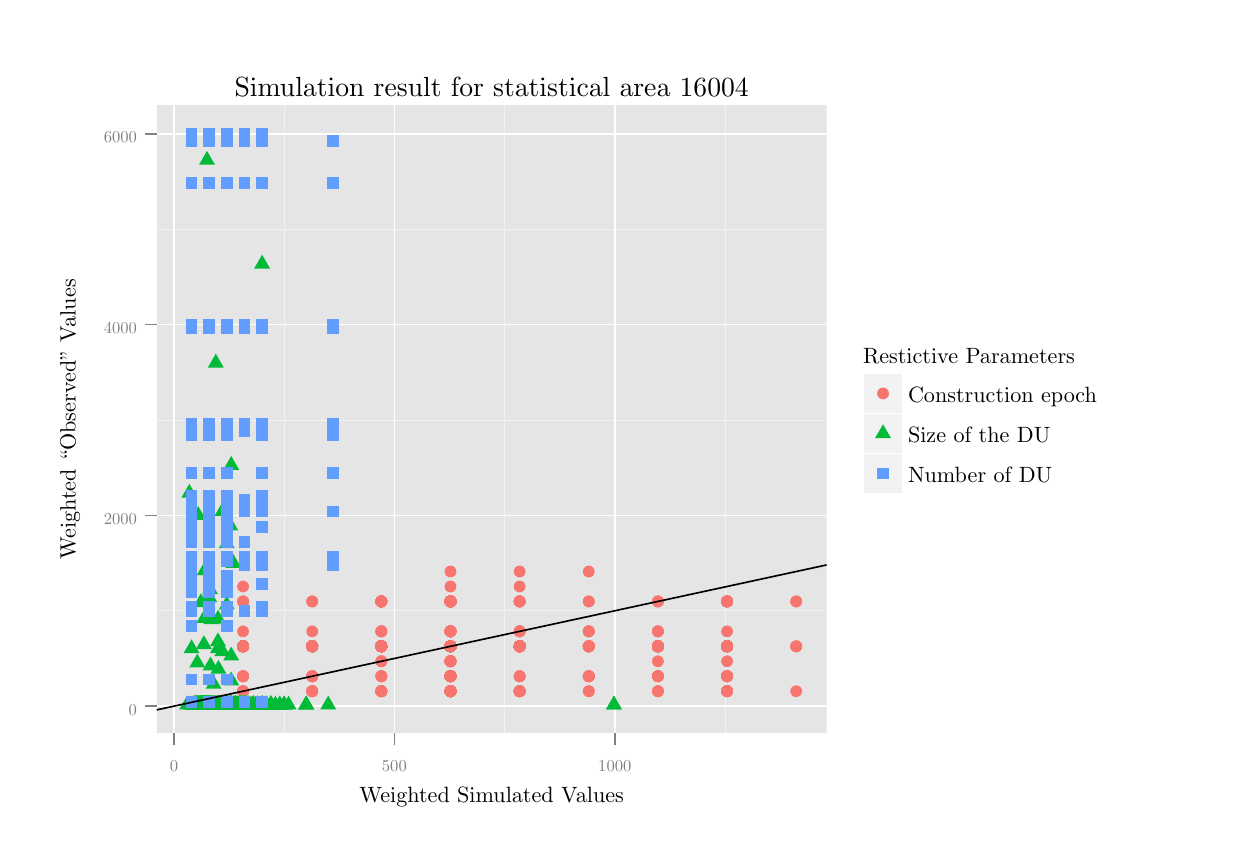
\begin{tikzpicture}[x=1pt,y=1pt]
\definecolor[named]{fillColor}{rgb}{1.00,1.00,1.00}
\path[use as bounding box,fill=fillColor,fill opacity=0.00] (0,0) rectangle (433.62,289.08);
\begin{scope}
\path[clip] (  0.00,  0.00) rectangle (433.62,289.08);
\definecolor[named]{drawColor}{rgb}{1.00,1.00,1.00}
\definecolor[named]{fillColor}{rgb}{1.00,1.00,1.00}

\path[draw=drawColor,line width= 0.6pt,line join=round,line cap=round,fill=fillColor] (  0.00,  0.00) rectangle (433.62,289.08);
\end{scope}
\begin{scope}
\path[clip] ( 46.62, 34.03) rectangle (288.71,261.09);
\definecolor[named]{fillColor}{rgb}{0.90,0.90,0.90}

\path[fill=fillColor] ( 46.62, 34.03) rectangle (288.71,261.09);
\definecolor[named]{drawColor}{rgb}{0.95,0.95,0.95}

\path[draw=drawColor,line width= 0.3pt,line join=round] ( 46.62, 78.38) --
	(288.71, 78.38);

\path[draw=drawColor,line width= 0.3pt,line join=round] ( 46.62,147.31) --
	(288.71,147.31);

\path[draw=drawColor,line width= 0.3pt,line join=round] ( 46.62,216.25) --
	(288.71,216.25);

\path[draw=drawColor,line width= 0.3pt,line join=round] ( 92.67, 34.03) --
	( 92.67,261.09);

\path[draw=drawColor,line width= 0.3pt,line join=round] (172.33, 34.03) --
	(172.33,261.09);

\path[draw=drawColor,line width= 0.3pt,line join=round] (251.98, 34.03) --
	(251.98,261.09);
\definecolor[named]{drawColor}{rgb}{1.00,1.00,1.00}

\path[draw=drawColor,line width= 0.6pt,line join=round] ( 46.62, 43.91) --
	(288.71, 43.91);

\path[draw=drawColor,line width= 0.6pt,line join=round] ( 46.62,112.84) --
	(288.71,112.84);

\path[draw=drawColor,line width= 0.6pt,line join=round] ( 46.62,181.78) --
	(288.71,181.78);

\path[draw=drawColor,line width= 0.6pt,line join=round] ( 46.62,250.72) --
	(288.71,250.72);

\path[draw=drawColor,line width= 0.6pt,line join=round] ( 52.84, 34.03) --
	( 52.84,261.09);

\path[draw=drawColor,line width= 0.6pt,line join=round] (132.50, 34.03) --
	(132.50,261.09);

\path[draw=drawColor,line width= 0.6pt,line join=round] (212.16, 34.03) --
	(212.16,261.09);
\definecolor[named]{fillColor}{rgb}{0.97,0.46,0.43}

\path[fill=fillColor] (227.74, 65.53) circle (  2.13);

\path[fill=fillColor] (177.77, 65.53) circle (  2.13);

\path[fill=fillColor] (152.78, 65.53) circle (  2.13);

\path[fill=fillColor] (227.74, 65.53) circle (  2.13);

\path[fill=fillColor] (202.75, 65.53) circle (  2.13);

\path[fill=fillColor] (152.78, 65.53) circle (  2.13);

\path[fill=fillColor] (177.77, 65.53) circle (  2.13);

\path[fill=fillColor] (152.78, 65.53) circle (  2.13);

\path[fill=fillColor] (152.78, 65.53) circle (  2.13);

\path[fill=fillColor] (202.75, 65.53) circle (  2.13);

\path[fill=fillColor] (152.78, 65.53) circle (  2.13);

\path[fill=fillColor] (127.80, 65.53) circle (  2.13);

\path[fill=fillColor] (152.78, 65.53) circle (  2.13);

\path[fill=fillColor] (127.80, 65.53) circle (  2.13);

\path[fill=fillColor] (152.78, 81.75) circle (  2.13);

\path[fill=fillColor] (152.78, 65.53) circle (  2.13);

\path[fill=fillColor] (152.78, 65.53) circle (  2.13);

\path[fill=fillColor] (152.78, 65.53) circle (  2.13);

\path[fill=fillColor] (127.80, 65.53) circle (  2.13);

\path[fill=fillColor] (127.80, 65.53) circle (  2.13);

\path[fill=fillColor] ( 77.83, 65.53) circle (  2.13);

\path[fill=fillColor] (152.78, 65.53) circle (  2.13);

\path[fill=fillColor] (177.77, 65.53) circle (  2.13);

\path[fill=fillColor] ( 77.83, 65.53) circle (  2.13);

\path[fill=fillColor] (227.74, 65.53) circle (  2.13);

\path[fill=fillColor] (152.78, 65.53) circle (  2.13);

\path[fill=fillColor] (152.78, 65.53) circle (  2.13);

\path[fill=fillColor] (127.80, 65.53) circle (  2.13);

\path[fill=fillColor] (152.78, 65.53) circle (  2.13);

\path[fill=fillColor] (152.78, 65.53) circle (  2.13);

\path[fill=fillColor] (177.77, 65.53) circle (  2.13);

\path[fill=fillColor] (152.78, 65.53) circle (  2.13);

\path[fill=fillColor] (227.74, 65.53) circle (  2.13);

\path[fill=fillColor] (152.78, 65.53) circle (  2.13);

\path[fill=fillColor] (152.78, 65.53) circle (  2.13);

\path[fill=fillColor] (152.78, 65.53) circle (  2.13);

\path[fill=fillColor] (152.78, 81.75) circle (  2.13);

\path[fill=fillColor] (152.78, 65.53) circle (  2.13);

\path[fill=fillColor] (152.78, 65.53) circle (  2.13);

\path[fill=fillColor] (152.78, 65.53) circle (  2.13);

\path[fill=fillColor] (227.74, 65.53) circle (  2.13);

\path[fill=fillColor] (127.80, 65.53) circle (  2.13);

\path[fill=fillColor] (127.80, 65.53) circle (  2.13);

\path[fill=fillColor] (177.77, 65.53) circle (  2.13);

\path[fill=fillColor] (152.78, 65.53) circle (  2.13);

\path[fill=fillColor] (177.77, 65.53) circle (  2.13);

\path[fill=fillColor] (127.80, 65.53) circle (  2.13);

\path[fill=fillColor] (152.78, 65.53) circle (  2.13);

\path[fill=fillColor] (152.78, 65.53) circle (  2.13);

\path[fill=fillColor] (152.78, 65.53) circle (  2.13);

\path[fill=fillColor] (102.81, 54.72) circle (  2.13);

\path[fill=fillColor] ( 77.83, 54.72) circle (  2.13);

\path[fill=fillColor] (152.78, 49.31) circle (  2.13);

\path[fill=fillColor] (252.72, 49.31) circle (  2.13);

\path[fill=fillColor] (152.78, 49.31) circle (  2.13);

\path[fill=fillColor] (127.80, 49.31) circle (  2.13);

\path[fill=fillColor] (102.81, 65.53) circle (  2.13);

\path[fill=fillColor] (252.72, 65.53) circle (  2.13);

\path[fill=fillColor] (152.78, 65.53) circle (  2.13);

\path[fill=fillColor] (252.72, 65.53) circle (  2.13);

\path[fill=fillColor] (252.72, 65.53) circle (  2.13);

\path[fill=fillColor] (227.74, 65.53) circle (  2.13);

\path[fill=fillColor] (177.77, 65.53) circle (  2.13);

\path[fill=fillColor] (227.74, 65.53) circle (  2.13);

\path[fill=fillColor] ( 77.83, 65.53) circle (  2.13);

\path[fill=fillColor] (177.77, 65.53) circle (  2.13);

\path[fill=fillColor] ( 77.83, 65.53) circle (  2.13);

\path[fill=fillColor] (177.77, 65.53) circle (  2.13);

\path[fill=fillColor] ( 77.83, 65.53) circle (  2.13);

\path[fill=fillColor] (152.78, 65.53) circle (  2.13);

\path[fill=fillColor] (252.72, 65.53) circle (  2.13);

\path[fill=fillColor] (177.77, 65.53) circle (  2.13);

\path[fill=fillColor] ( 77.83, 65.53) circle (  2.13);

\path[fill=fillColor] (152.78, 65.53) circle (  2.13);

\path[fill=fillColor] (152.78, 65.53) circle (  2.13);

\path[fill=fillColor] (102.81, 65.53) circle (  2.13);

\path[fill=fillColor] (102.81, 65.53) circle (  2.13);

\path[fill=fillColor] (102.81, 65.53) circle (  2.13);

\path[fill=fillColor] (177.77, 65.53) circle (  2.13);

\path[fill=fillColor] (127.80, 65.53) circle (  2.13);

\path[fill=fillColor] (127.80, 65.53) circle (  2.13);

\path[fill=fillColor] (252.72, 65.53) circle (  2.13);

\path[fill=fillColor] (152.78, 65.53) circle (  2.13);

\path[fill=fillColor] (152.78, 65.53) circle (  2.13);

\path[fill=fillColor] (277.71, 65.53) circle (  2.13);

\path[fill=fillColor] (152.78, 65.53) circle (  2.13);

\path[fill=fillColor] ( 77.83, 65.53) circle (  2.13);

\path[fill=fillColor] (152.78, 65.53) circle (  2.13);

\path[fill=fillColor] (227.74, 65.53) circle (  2.13);

\path[fill=fillColor] (177.77, 65.53) circle (  2.13);

\path[fill=fillColor] ( 77.83, 65.53) circle (  2.13);

\path[fill=fillColor] (202.75, 65.53) circle (  2.13);

\path[fill=fillColor] ( 77.83, 87.15) circle (  2.13);

\path[fill=fillColor] ( 77.83, 65.53) circle (  2.13);

\path[fill=fillColor] (227.74, 65.53) circle (  2.13);

\path[fill=fillColor] (152.78, 65.53) circle (  2.13);

\path[fill=fillColor] (152.78, 65.53) circle (  2.13);

\path[fill=fillColor] (227.74, 65.53) circle (  2.13);

\path[fill=fillColor] (177.77, 65.53) circle (  2.13);

\path[fill=fillColor] (127.80, 65.53) circle (  2.13);

\path[fill=fillColor] (177.77, 65.53) circle (  2.13);

\path[fill=fillColor] (177.77, 65.53) circle (  2.13);

\path[fill=fillColor] (127.80, 65.53) circle (  2.13);

\path[fill=fillColor] (152.78, 65.53) circle (  2.13);

\path[fill=fillColor] ( 77.83, 65.53) circle (  2.13);

\path[fill=fillColor] (252.72, 65.53) circle (  2.13);

\path[fill=fillColor] (127.80, 65.53) circle (  2.13);

\path[fill=fillColor] (152.78, 65.53) circle (  2.13);

\path[fill=fillColor] (152.78, 65.53) circle (  2.13);

\path[fill=fillColor] (152.78, 65.53) circle (  2.13);

\path[fill=fillColor] ( 77.83, 65.53) circle (  2.13);

\path[fill=fillColor] (152.78, 65.53) circle (  2.13);

\path[fill=fillColor] (152.78, 65.53) circle (  2.13);

\path[fill=fillColor] (202.75, 65.53) circle (  2.13);

\path[fill=fillColor] (152.78, 65.53) circle (  2.13);

\path[fill=fillColor] (152.78, 65.53) circle (  2.13);

\path[fill=fillColor] (152.78, 65.53) circle (  2.13);

\path[fill=fillColor] (152.78, 65.53) circle (  2.13);

\path[fill=fillColor] (152.78, 65.53) circle (  2.13);

\path[fill=fillColor] (127.80, 65.53) circle (  2.13);

\path[fill=fillColor] (227.74, 65.53) circle (  2.13);

\path[fill=fillColor] (102.81, 65.53) circle (  2.13);

\path[fill=fillColor] (152.78, 65.53) circle (  2.13);

\path[fill=fillColor] (102.81, 65.53) circle (  2.13);

\path[fill=fillColor] (152.78, 65.53) circle (  2.13);

\path[fill=fillColor] (152.78, 65.53) circle (  2.13);

\path[fill=fillColor] (102.81, 65.53) circle (  2.13);

\path[fill=fillColor] (152.78, 65.53) circle (  2.13);

\path[fill=fillColor] (102.81, 65.53) circle (  2.13);

\path[fill=fillColor] (177.77, 65.53) circle (  2.13);

\path[fill=fillColor] (177.77, 65.53) circle (  2.13);

\path[fill=fillColor] (177.77, 65.53) circle (  2.13);

\path[fill=fillColor] (152.78, 65.53) circle (  2.13);

\path[fill=fillColor] (152.78, 65.53) circle (  2.13);

\path[fill=fillColor] (152.78, 65.53) circle (  2.13);

\path[fill=fillColor] (152.78, 65.53) circle (  2.13);

\path[fill=fillColor] (152.78, 65.53) circle (  2.13);

\path[fill=fillColor] ( 77.83, 65.53) circle (  2.13);

\path[fill=fillColor] (227.74, 65.53) circle (  2.13);

\path[fill=fillColor] (152.78, 65.53) circle (  2.13);

\path[fill=fillColor] (127.80, 65.53) circle (  2.13);

\path[fill=fillColor] (152.78, 65.53) circle (  2.13);

\path[fill=fillColor] (152.78, 65.53) circle (  2.13);

\path[fill=fillColor] (127.80, 65.53) circle (  2.13);

\path[fill=fillColor] (177.77, 65.53) circle (  2.13);

\path[fill=fillColor] (127.80, 65.53) circle (  2.13);

\path[fill=fillColor] (152.78, 65.53) circle (  2.13);

\path[fill=fillColor] (177.77, 65.53) circle (  2.13);

\path[fill=fillColor] (252.72, 65.53) circle (  2.13);

\path[fill=fillColor] (152.78, 65.53) circle (  2.13);

\path[fill=fillColor] (102.81, 65.53) circle (  2.13);

\path[fill=fillColor] (152.78, 65.53) circle (  2.13);

\path[fill=fillColor] (152.78, 65.53) circle (  2.13);

\path[fill=fillColor] (227.74, 65.53) circle (  2.13);

\path[fill=fillColor] (102.81, 65.53) circle (  2.13);

\path[fill=fillColor] (152.78, 65.53) circle (  2.13);

\path[fill=fillColor] (152.78, 65.53) circle (  2.13);

\path[fill=fillColor] (102.81, 65.53) circle (  2.13);

\path[fill=fillColor] (152.78, 65.53) circle (  2.13);

\path[fill=fillColor] (152.78, 65.53) circle (  2.13);

\path[fill=fillColor] (152.78, 65.53) circle (  2.13);

\path[fill=fillColor] (152.78, 65.53) circle (  2.13);

\path[fill=fillColor] (152.78, 65.53) circle (  2.13);

\path[fill=fillColor] (152.78, 65.53) circle (  2.13);

\path[fill=fillColor] (152.78, 65.53) circle (  2.13);

\path[fill=fillColor] (152.78, 65.53) circle (  2.13);

\path[fill=fillColor] (102.81, 65.53) circle (  2.13);

\path[fill=fillColor] (177.77, 65.53) circle (  2.13);

\path[fill=fillColor] (152.78, 65.53) circle (  2.13);

\path[fill=fillColor] (152.78, 65.53) circle (  2.13);

\path[fill=fillColor] (252.72, 65.53) circle (  2.13);

\path[fill=fillColor] (152.78, 65.53) circle (  2.13);

\path[fill=fillColor] (152.78, 65.53) circle (  2.13);

\path[fill=fillColor] (102.81, 65.53) circle (  2.13);

\path[fill=fillColor] (152.78, 65.53) circle (  2.13);

\path[fill=fillColor] (152.78, 65.53) circle (  2.13);

\path[fill=fillColor] (152.78, 65.53) circle (  2.13);

\path[fill=fillColor] (127.80, 65.53) circle (  2.13);

\path[fill=fillColor] (102.81, 65.53) circle (  2.13);

\path[fill=fillColor] (152.78, 65.53) circle (  2.13);

\path[fill=fillColor] (127.80, 65.53) circle (  2.13);

\path[fill=fillColor] (227.74, 65.53) circle (  2.13);

\path[fill=fillColor] (127.80, 65.53) circle (  2.13);

\path[fill=fillColor] (152.78, 65.53) circle (  2.13);

\path[fill=fillColor] ( 77.83, 65.53) circle (  2.13);

\path[fill=fillColor] (177.77, 65.53) circle (  2.13);

\path[fill=fillColor] (177.77, 65.53) circle (  2.13);

\path[fill=fillColor] (152.78, 65.53) circle (  2.13);

\path[fill=fillColor] (152.78, 65.53) circle (  2.13);

\path[fill=fillColor] (152.78, 65.53) circle (  2.13);

\path[fill=fillColor] (202.75, 65.53) circle (  2.13);

\path[fill=fillColor] (127.80, 65.53) circle (  2.13);

\path[fill=fillColor] (102.81, 65.53) circle (  2.13);

\path[fill=fillColor] (177.77, 65.53) circle (  2.13);

\path[fill=fillColor] (177.77, 65.53) circle (  2.13);

\path[fill=fillColor] (152.78, 65.53) circle (  2.13);

\path[fill=fillColor] (227.74, 65.53) circle (  2.13);

\path[fill=fillColor] (127.80, 65.53) circle (  2.13);

\path[fill=fillColor] (252.72, 65.53) circle (  2.13);

\path[fill=fillColor] (152.78, 65.53) circle (  2.13);

\path[fill=fillColor] ( 77.83, 65.53) circle (  2.13);

\path[fill=fillColor] (152.78, 65.53) circle (  2.13);

\path[fill=fillColor] (152.78, 65.53) circle (  2.13);

\path[fill=fillColor] (227.74, 65.53) circle (  2.13);

\path[fill=fillColor] (152.78, 65.53) circle (  2.13);

\path[fill=fillColor] (152.78, 65.53) circle (  2.13);

\path[fill=fillColor] (252.72, 65.53) circle (  2.13);

\path[fill=fillColor] ( 77.83, 65.53) circle (  2.13);

\path[fill=fillColor] (127.80, 65.53) circle (  2.13);

\path[fill=fillColor] (152.78, 65.53) circle (  2.13);

\path[fill=fillColor] (152.78, 65.53) circle (  2.13);

\path[fill=fillColor] (152.78, 65.53) circle (  2.13);

\path[fill=fillColor] (152.78, 65.53) circle (  2.13);

\path[fill=fillColor] (102.81, 65.53) circle (  2.13);

\path[fill=fillColor] (252.72, 65.53) circle (  2.13);

\path[fill=fillColor] (252.72, 65.53) circle (  2.13);

\path[fill=fillColor] (177.77, 65.53) circle (  2.13);

\path[fill=fillColor] (152.78, 65.53) circle (  2.13);

\path[fill=fillColor] (177.77, 65.53) circle (  2.13);

\path[fill=fillColor] (152.78, 65.53) circle (  2.13);

\path[fill=fillColor] (152.78, 65.53) circle (  2.13);

\path[fill=fillColor] (152.78, 65.53) circle (  2.13);

\path[fill=fillColor] (102.81, 65.53) circle (  2.13);

\path[fill=fillColor] (252.72, 65.53) circle (  2.13);

\path[fill=fillColor] (152.78, 65.53) circle (  2.13);

\path[fill=fillColor] (152.78, 65.53) circle (  2.13);

\path[fill=fillColor] (127.80, 65.53) circle (  2.13);

\path[fill=fillColor] ( 77.83, 65.53) circle (  2.13);

\path[fill=fillColor] (252.72, 65.53) circle (  2.13);

\path[fill=fillColor] (152.78, 65.53) circle (  2.13);

\path[fill=fillColor] (152.78, 81.75) circle (  2.13);

\path[fill=fillColor] (202.75, 92.56) circle (  2.13);

\path[fill=fillColor] (252.72, 65.53) circle (  2.13);

\path[fill=fillColor] (227.74, 65.53) circle (  2.13);

\path[fill=fillColor] (127.80, 65.53) circle (  2.13);

\path[fill=fillColor] (227.74, 65.53) circle (  2.13);

\path[fill=fillColor] (152.78, 65.53) circle (  2.13);

\path[fill=fillColor] (252.72, 65.53) circle (  2.13);

\path[fill=fillColor] (127.80, 65.53) circle (  2.13);

\path[fill=fillColor] (127.80, 65.53) circle (  2.13);

\path[fill=fillColor] (152.78, 70.94) circle (  2.13);

\path[fill=fillColor] (177.77, 70.94) circle (  2.13);

\path[fill=fillColor] (202.75, 49.31) circle (  2.13);

\path[fill=fillColor] (177.77, 87.15) circle (  2.13);

\path[fill=fillColor] (252.72, 65.53) circle (  2.13);

\path[fill=fillColor] (252.72, 65.53) circle (  2.13);

\path[fill=fillColor] (152.78, 65.53) circle (  2.13);

\path[fill=fillColor] (152.78, 65.53) circle (  2.13);

\path[fill=fillColor] (102.81, 65.53) circle (  2.13);

\path[fill=fillColor] (152.78, 65.53) circle (  2.13);

\path[fill=fillColor] (152.78, 65.53) circle (  2.13);

\path[fill=fillColor] (127.80, 65.53) circle (  2.13);

\path[fill=fillColor] (127.80, 65.53) circle (  2.13);

\path[fill=fillColor] (127.80, 65.53) circle (  2.13);

\path[fill=fillColor] (152.78, 65.53) circle (  2.13);

\path[fill=fillColor] (102.81, 65.53) circle (  2.13);

\path[fill=fillColor] (152.78, 65.53) circle (  2.13);

\path[fill=fillColor] (177.77, 65.53) circle (  2.13);

\path[fill=fillColor] (152.78, 65.53) circle (  2.13);

\path[fill=fillColor] (177.77, 65.53) circle (  2.13);

\path[fill=fillColor] (227.74, 65.53) circle (  2.13);

\path[fill=fillColor] (177.77, 65.53) circle (  2.13);

\path[fill=fillColor] (227.74, 65.53) circle (  2.13);

\path[fill=fillColor] (177.77, 65.53) circle (  2.13);

\path[fill=fillColor] (177.77, 65.53) circle (  2.13);

\path[fill=fillColor] (177.77, 92.56) circle (  2.13);

\path[fill=fillColor] (177.77, 65.53) circle (  2.13);

\path[fill=fillColor] (252.72, 65.53) circle (  2.13);

\path[fill=fillColor] ( 77.83, 65.53) circle (  2.13);

\path[fill=fillColor] (227.74, 65.53) circle (  2.13);

\path[fill=fillColor] (152.78, 65.53) circle (  2.13);

\path[fill=fillColor] (152.78, 65.53) circle (  2.13);

\path[fill=fillColor] (152.78, 65.53) circle (  2.13);

\path[fill=fillColor] (252.72, 65.53) circle (  2.13);

\path[fill=fillColor] (152.78, 65.53) circle (  2.13);

\path[fill=fillColor] (102.81, 65.53) circle (  2.13);

\path[fill=fillColor] ( 77.83, 65.53) circle (  2.13);

\path[fill=fillColor] (152.78, 65.53) circle (  2.13);

\path[fill=fillColor] (252.72, 65.53) circle (  2.13);

\path[fill=fillColor] ( 77.83, 65.53) circle (  2.13);

\path[fill=fillColor] ( 77.83, 65.53) circle (  2.13);

\path[fill=fillColor] (127.80, 65.53) circle (  2.13);

\path[fill=fillColor] (127.80, 81.75) circle (  2.13);

\path[fill=fillColor] (152.78, 65.53) circle (  2.13);

\path[fill=fillColor] (152.78, 65.53) circle (  2.13);

\path[fill=fillColor] (102.81, 65.53) circle (  2.13);

\path[fill=fillColor] (152.78, 65.53) circle (  2.13);

\path[fill=fillColor] (252.72, 65.53) circle (  2.13);

\path[fill=fillColor] (152.78, 65.53) circle (  2.13);

\path[fill=fillColor] (152.78, 65.53) circle (  2.13);

\path[fill=fillColor] (152.78, 65.53) circle (  2.13);

\path[fill=fillColor] (127.80, 65.53) circle (  2.13);

\path[fill=fillColor] (127.80, 65.53) circle (  2.13);

\path[fill=fillColor] (252.72, 65.53) circle (  2.13);

\path[fill=fillColor] ( 77.83, 65.53) circle (  2.13);

\path[fill=fillColor] (152.78, 65.53) circle (  2.13);

\path[fill=fillColor] (152.78, 65.53) circle (  2.13);

\path[fill=fillColor] (127.80, 65.53) circle (  2.13);

\path[fill=fillColor] (177.77, 49.31) circle (  2.13);

\path[fill=fillColor] (152.78, 49.31) circle (  2.13);

\path[fill=fillColor] (152.78, 49.31) circle (  2.13);

\path[fill=fillColor] (152.78, 49.31) circle (  2.13);

\path[fill=fillColor] (177.77, 49.31) circle (  2.13);

\path[fill=fillColor] (152.78, 49.31) circle (  2.13);

\path[fill=fillColor] (127.80, 49.31) circle (  2.13);

\path[fill=fillColor] (152.78, 49.31) circle (  2.13);

\path[fill=fillColor] (252.72, 49.31) circle (  2.13);

\path[fill=fillColor] (252.72, 49.31) circle (  2.13);

\path[fill=fillColor] (252.72, 49.31) circle (  2.13);

\path[fill=fillColor] (127.80, 49.31) circle (  2.13);

\path[fill=fillColor] (127.80, 49.31) circle (  2.13);

\path[fill=fillColor] (102.81, 49.31) circle (  2.13);

\path[fill=fillColor] (102.81, 49.31) circle (  2.13);

\path[fill=fillColor] (152.78, 49.31) circle (  2.13);

\path[fill=fillColor] (252.72, 49.31) circle (  2.13);

\path[fill=fillColor] (152.78, 49.31) circle (  2.13);

\path[fill=fillColor] (177.77, 49.31) circle (  2.13);

\path[fill=fillColor] (127.80, 49.31) circle (  2.13);

\path[fill=fillColor] (127.80, 81.75) circle (  2.13);

\path[fill=fillColor] (252.72, 81.75) circle (  2.13);

\path[fill=fillColor] (152.78, 81.75) circle (  2.13);

\path[fill=fillColor] (177.77, 81.75) circle (  2.13);

\path[fill=fillColor] (152.78, 81.75) circle (  2.13);

\path[fill=fillColor] (127.80, 81.75) circle (  2.13);

\path[fill=fillColor] (277.71, 81.75) circle (  2.13);

\path[fill=fillColor] (152.78, 81.75) circle (  2.13);

\path[fill=fillColor] (152.78, 81.75) circle (  2.13);

\path[fill=fillColor] (152.78, 81.75) circle (  2.13);

\path[fill=fillColor] (152.78, 81.75) circle (  2.13);

\path[fill=fillColor] (252.72, 81.75) circle (  2.13);

\path[fill=fillColor] (127.80, 81.75) circle (  2.13);

\path[fill=fillColor] (252.72, 81.75) circle (  2.13);

\path[fill=fillColor] (202.75, 81.75) circle (  2.13);

\path[fill=fillColor] (152.78, 81.75) circle (  2.13);

\path[fill=fillColor] (152.78, 81.75) circle (  2.13);

\path[fill=fillColor] (152.78, 81.75) circle (  2.13);

\path[fill=fillColor] (227.74, 81.75) circle (  2.13);

\path[fill=fillColor] (152.78, 81.75) circle (  2.13);

\path[fill=fillColor] (252.72, 81.75) circle (  2.13);

\path[fill=fillColor] (177.77, 81.75) circle (  2.13);

\path[fill=fillColor] (127.80, 81.75) circle (  2.13);

\path[fill=fillColor] (152.78, 81.75) circle (  2.13);

\path[fill=fillColor] (152.78, 81.75) circle (  2.13);

\path[fill=fillColor] (202.75, 81.75) circle (  2.13);

\path[fill=fillColor] (177.77, 81.75) circle (  2.13);

\path[fill=fillColor] (152.78, 81.75) circle (  2.13);

\path[fill=fillColor] (252.72, 81.75) circle (  2.13);

\path[fill=fillColor] (152.78, 81.75) circle (  2.13);

\path[fill=fillColor] (152.78, 81.75) circle (  2.13);

\path[fill=fillColor] (152.78, 81.75) circle (  2.13);

\path[fill=fillColor] (102.81, 81.75) circle (  2.13);

\path[fill=fillColor] (152.78, 81.75) circle (  2.13);

\path[fill=fillColor] (127.80, 81.75) circle (  2.13);

\path[fill=fillColor] (227.74, 81.75) circle (  2.13);

\path[fill=fillColor] (152.78, 81.75) circle (  2.13);

\path[fill=fillColor] (152.78, 81.75) circle (  2.13);

\path[fill=fillColor] (252.72, 81.75) circle (  2.13);

\path[fill=fillColor] (252.72, 81.75) circle (  2.13);

\path[fill=fillColor] (127.80, 81.75) circle (  2.13);

\path[fill=fillColor] (127.80, 81.75) circle (  2.13);

\path[fill=fillColor] (102.81, 81.75) circle (  2.13);

\path[fill=fillColor] (277.71, 81.75) circle (  2.13);

\path[fill=fillColor] ( 77.83, 81.75) circle (  2.13);

\path[fill=fillColor] (152.78, 81.75) circle (  2.13);

\path[fill=fillColor] (127.80, 81.75) circle (  2.13);

\path[fill=fillColor] (177.77, 81.75) circle (  2.13);

\path[fill=fillColor] (127.80, 81.75) circle (  2.13);

\path[fill=fillColor] (252.72, 81.75) circle (  2.13);

\path[fill=fillColor] (152.78, 92.56) circle (  2.13);

\path[fill=fillColor] (152.78, 65.53) circle (  2.13);

\path[fill=fillColor] (102.81, 65.53) circle (  2.13);

\path[fill=fillColor] ( 77.83, 65.53) circle (  2.13);

\path[fill=fillColor] (152.78, 65.53) circle (  2.13);

\path[fill=fillColor] (252.72, 65.53) circle (  2.13);

\path[fill=fillColor] (127.80, 65.53) circle (  2.13);

\path[fill=fillColor] (202.75, 65.53) circle (  2.13);

\path[fill=fillColor] (227.74, 65.53) circle (  2.13);

\path[fill=fillColor] (227.74, 65.53) circle (  2.13);

\path[fill=fillColor] (177.77, 65.53) circle (  2.13);

\path[fill=fillColor] (227.74, 65.53) circle (  2.13);

\path[fill=fillColor] (227.74, 65.53) circle (  2.13);

\path[fill=fillColor] (152.78, 65.53) circle (  2.13);

\path[fill=fillColor] (152.78, 65.53) circle (  2.13);

\path[fill=fillColor] (152.78, 65.53) circle (  2.13);

\path[fill=fillColor] ( 77.83, 65.53) circle (  2.13);

\path[fill=fillColor] (177.77, 65.53) circle (  2.13);

\path[fill=fillColor] (227.74, 65.53) circle (  2.13);

\path[fill=fillColor] ( 77.83, 65.53) circle (  2.13);

\path[fill=fillColor] (102.81, 65.53) circle (  2.13);

\path[fill=fillColor] (102.81, 65.53) circle (  2.13);

\path[fill=fillColor] (127.80, 65.53) circle (  2.13);

\path[fill=fillColor] ( 77.83, 65.53) circle (  2.13);

\path[fill=fillColor] (177.77, 65.53) circle (  2.13);

\path[fill=fillColor] (177.77, 65.53) circle (  2.13);

\path[fill=fillColor] (177.77, 65.53) circle (  2.13);

\path[fill=fillColor] ( 77.83, 65.53) circle (  2.13);

\path[fill=fillColor] (127.80, 49.31) circle (  2.13);

\path[fill=fillColor] (152.78, 49.31) circle (  2.13);

\path[fill=fillColor] (202.75, 49.31) circle (  2.13);

\path[fill=fillColor] (152.78, 49.31) circle (  2.13);

\path[fill=fillColor] (152.78, 49.31) circle (  2.13);

\path[fill=fillColor] (177.77, 49.31) circle (  2.13);

\path[fill=fillColor] (127.80, 49.31) circle (  2.13);

\path[fill=fillColor] (102.81, 49.31) circle (  2.13);

\path[fill=fillColor] (252.72, 49.31) circle (  2.13);

\path[fill=fillColor] (177.77, 49.31) circle (  2.13);

\path[fill=fillColor] (127.80, 49.31) circle (  2.13);

\path[fill=fillColor] ( 77.83, 49.31) circle (  2.13);

\path[fill=fillColor] (177.77, 49.31) circle (  2.13);

\path[fill=fillColor] (152.78, 49.31) circle (  2.13);

\path[fill=fillColor] (227.74, 49.31) circle (  2.13);

\path[fill=fillColor] (102.81, 49.31) circle (  2.13);

\path[fill=fillColor] (152.78, 49.31) circle (  2.13);

\path[fill=fillColor] (127.80, 49.31) circle (  2.13);

\path[fill=fillColor] (152.78, 49.31) circle (  2.13);

\path[fill=fillColor] (152.78, 49.31) circle (  2.13);

\path[fill=fillColor] (177.77, 49.31) circle (  2.13);

\path[fill=fillColor] (152.78, 49.31) circle (  2.13);

\path[fill=fillColor] (152.78, 49.31) circle (  2.13);

\path[fill=fillColor] (152.78, 49.31) circle (  2.13);

\path[fill=fillColor] (127.80, 49.31) circle (  2.13);

\path[fill=fillColor] (252.72, 49.31) circle (  2.13);

\path[fill=fillColor] (252.72, 49.31) circle (  2.13);

\path[fill=fillColor] (177.77, 49.31) circle (  2.13);

\path[fill=fillColor] (152.78, 49.31) circle (  2.13);

\path[fill=fillColor] (152.78, 49.31) circle (  2.13);

\path[fill=fillColor] (177.77, 49.31) circle (  2.13);

\path[fill=fillColor] (127.80, 49.31) circle (  2.13);

\path[fill=fillColor] (152.78, 49.31) circle (  2.13);

\path[fill=fillColor] (152.78, 49.31) circle (  2.13);

\path[fill=fillColor] (227.74, 49.31) circle (  2.13);

\path[fill=fillColor] (102.81, 49.31) circle (  2.13);

\path[fill=fillColor] (177.77, 49.31) circle (  2.13);

\path[fill=fillColor] (177.77, 49.31) circle (  2.13);

\path[fill=fillColor] (152.78, 49.31) circle (  2.13);

\path[fill=fillColor] (252.72, 65.53) circle (  2.13);

\path[fill=fillColor] ( 77.83, 65.53) circle (  2.13);

\path[fill=fillColor] (152.78, 65.53) circle (  2.13);

\path[fill=fillColor] ( 77.83, 65.53) circle (  2.13);

\path[fill=fillColor] (227.74, 65.53) circle (  2.13);

\path[fill=fillColor] (127.80, 65.53) circle (  2.13);

\path[fill=fillColor] (127.80, 65.53) circle (  2.13);

\path[fill=fillColor] ( 77.83, 65.53) circle (  2.13);

\path[fill=fillColor] (152.78, 65.53) circle (  2.13);

\path[fill=fillColor] ( 77.83, 65.53) circle (  2.13);

\path[fill=fillColor] (152.78, 65.53) circle (  2.13);

\path[fill=fillColor] ( 77.83, 65.53) circle (  2.13);

\path[fill=fillColor] (127.80, 65.53) circle (  2.13);

\path[fill=fillColor] (152.78, 65.53) circle (  2.13);

\path[fill=fillColor] (152.78, 65.53) circle (  2.13);

\path[fill=fillColor] (227.74, 65.53) circle (  2.13);

\path[fill=fillColor] (177.77, 65.53) circle (  2.13);

\path[fill=fillColor] (102.81, 65.53) circle (  2.13);

\path[fill=fillColor] (277.71, 65.53) circle (  2.13);

\path[fill=fillColor] (152.78, 65.53) circle (  2.13);

\path[fill=fillColor] (102.81, 65.53) circle (  2.13);

\path[fill=fillColor] (177.77, 65.53) circle (  2.13);

\path[fill=fillColor] (152.78, 65.53) circle (  2.13);

\path[fill=fillColor] (127.80, 65.53) circle (  2.13);

\path[fill=fillColor] ( 77.83, 65.53) circle (  2.13);

\path[fill=fillColor] (152.78, 65.53) circle (  2.13);

\path[fill=fillColor] (152.78, 65.53) circle (  2.13);

\path[fill=fillColor] (152.78, 65.53) circle (  2.13);

\path[fill=fillColor] (177.77, 65.53) circle (  2.13);

\path[fill=fillColor] (102.81, 65.53) circle (  2.13);

\path[fill=fillColor] (152.78, 65.53) circle (  2.13);

\path[fill=fillColor] (127.80, 65.53) circle (  2.13);

\path[fill=fillColor] (152.78, 65.53) circle (  2.13);

\path[fill=fillColor] (252.72, 65.53) circle (  2.13);

\path[fill=fillColor] (152.78, 65.53) circle (  2.13);

\path[fill=fillColor] (152.78, 65.53) circle (  2.13);

\path[fill=fillColor] (152.78, 65.53) circle (  2.13);

\path[fill=fillColor] (252.72, 70.94) circle (  2.13);

\path[fill=fillColor] (102.81, 54.72) circle (  2.13);

\path[fill=fillColor] (127.80, 54.72) circle (  2.13);

\path[fill=fillColor] (152.78, 54.72) circle (  2.13);

\path[fill=fillColor] (227.74, 54.72) circle (  2.13);

\path[fill=fillColor] (252.72, 54.72) circle (  2.13);

\path[fill=fillColor] (227.74, 65.53) circle (  2.13);

\path[fill=fillColor] (252.72, 65.53) circle (  2.13);

\path[fill=fillColor] (227.74, 65.53) circle (  2.13);

\path[fill=fillColor] (252.72, 65.53) circle (  2.13);

\path[fill=fillColor] (152.78, 65.53) circle (  2.13);

\path[fill=fillColor] (127.80, 65.53) circle (  2.13);

\path[fill=fillColor] ( 77.83, 65.53) circle (  2.13);

\path[fill=fillColor] (252.72, 65.53) circle (  2.13);

\path[fill=fillColor] (152.78, 65.53) circle (  2.13);

\path[fill=fillColor] (177.77, 65.53) circle (  2.13);

\path[fill=fillColor] (252.72, 65.53) circle (  2.13);

\path[fill=fillColor] (177.77, 65.53) circle (  2.13);

\path[fill=fillColor] (227.74, 65.53) circle (  2.13);

\path[fill=fillColor] (152.78, 65.53) circle (  2.13);

\path[fill=fillColor] ( 77.83, 65.53) circle (  2.13);

\path[fill=fillColor] (202.75, 65.53) circle (  2.13);

\path[fill=fillColor] (102.81, 65.53) circle (  2.13);

\path[fill=fillColor] (202.75, 65.53) circle (  2.13);

\path[fill=fillColor] (177.77, 65.53) circle (  2.13);

\path[fill=fillColor] (202.75, 65.53) circle (  2.13);

\path[fill=fillColor] (152.78, 65.53) circle (  2.13);

\path[fill=fillColor] (152.78, 87.15) circle (  2.13);

\path[fill=fillColor] (127.80, 81.75) circle (  2.13);

\path[fill=fillColor] (152.78, 81.75) circle (  2.13);

\path[fill=fillColor] (127.80, 65.53) circle (  2.13);

\path[fill=fillColor] (152.78, 65.53) circle (  2.13);

\path[fill=fillColor] (152.78, 65.53) circle (  2.13);

\path[fill=fillColor] (152.78, 65.53) circle (  2.13);

\path[fill=fillColor] (127.80, 65.53) circle (  2.13);

\path[fill=fillColor] (127.80, 65.53) circle (  2.13);

\path[fill=fillColor] (152.78, 65.53) circle (  2.13);

\path[fill=fillColor] (152.78, 65.53) circle (  2.13);

\path[fill=fillColor] (202.75, 65.53) circle (  2.13);

\path[fill=fillColor] (277.71, 65.53) circle (  2.13);

\path[fill=fillColor] (152.78, 65.53) circle (  2.13);

\path[fill=fillColor] (252.72, 65.53) circle (  2.13);

\path[fill=fillColor] (152.78, 65.53) circle (  2.13);

\path[fill=fillColor] (152.78, 65.53) circle (  2.13);

\path[fill=fillColor] ( 77.83, 65.53) circle (  2.13);

\path[fill=fillColor] (152.78, 65.53) circle (  2.13);

\path[fill=fillColor] (152.78, 65.53) circle (  2.13);

\path[fill=fillColor] (152.78, 65.53) circle (  2.13);

\path[fill=fillColor] (127.80, 65.53) circle (  2.13);

\path[fill=fillColor] (202.75, 65.53) circle (  2.13);

\path[fill=fillColor] (152.78, 65.53) circle (  2.13);

\path[fill=fillColor] (127.80, 65.53) circle (  2.13);

\path[fill=fillColor] (152.78, 65.53) circle (  2.13);

\path[fill=fillColor] (102.81, 65.53) circle (  2.13);

\path[fill=fillColor] (127.80, 65.53) circle (  2.13);

\path[fill=fillColor] (152.78, 65.53) circle (  2.13);

\path[fill=fillColor] ( 77.83, 65.53) circle (  2.13);

\path[fill=fillColor] (227.74, 65.53) circle (  2.13);

\path[fill=fillColor] (102.81, 54.72) circle (  2.13);

\path[fill=fillColor] (227.74, 54.72) circle (  2.13);

\path[fill=fillColor] (152.78, 54.72) circle (  2.13);

\path[fill=fillColor] (152.78, 54.72) circle (  2.13);

\path[fill=fillColor] (152.78, 54.72) circle (  2.13);

\path[fill=fillColor] (252.72, 54.72) circle (  2.13);

\path[fill=fillColor] (227.74, 54.72) circle (  2.13);

\path[fill=fillColor] (227.74, 54.72) circle (  2.13);

\path[fill=fillColor] (127.80, 54.72) circle (  2.13);

\path[fill=fillColor] (152.78, 54.72) circle (  2.13);

\path[fill=fillColor] (252.72, 54.72) circle (  2.13);

\path[fill=fillColor] (152.78, 54.72) circle (  2.13);

\path[fill=fillColor] ( 77.83, 54.72) circle (  2.13);

\path[fill=fillColor] ( 77.83, 54.72) circle (  2.13);

\path[fill=fillColor] (152.78, 54.72) circle (  2.13);

\path[fill=fillColor] (102.81, 54.72) circle (  2.13);

\path[fill=fillColor] (152.78, 54.72) circle (  2.13);

\path[fill=fillColor] (152.78, 54.72) circle (  2.13);

\path[fill=fillColor] (152.78, 54.72) circle (  2.13);

\path[fill=fillColor] (252.72, 54.72) circle (  2.13);

\path[fill=fillColor] ( 77.83, 54.72) circle (  2.13);

\path[fill=fillColor] (102.81, 54.72) circle (  2.13);

\path[fill=fillColor] (152.78, 54.72) circle (  2.13);

\path[fill=fillColor] (152.78, 54.72) circle (  2.13);

\path[fill=fillColor] (152.78, 54.72) circle (  2.13);

\path[fill=fillColor] (202.75, 54.72) circle (  2.13);

\path[fill=fillColor] (152.78, 54.72) circle (  2.13);

\path[fill=fillColor] (177.77, 54.72) circle (  2.13);

\path[fill=fillColor] (252.72, 54.72) circle (  2.13);

\path[fill=fillColor] (177.77, 54.72) circle (  2.13);

\path[fill=fillColor] (152.78, 54.72) circle (  2.13);

\path[fill=fillColor] (227.74, 54.72) circle (  2.13);

\path[fill=fillColor] (152.78, 54.72) circle (  2.13);

\path[fill=fillColor] (252.72, 54.72) circle (  2.13);

\path[fill=fillColor] (252.72, 54.72) circle (  2.13);

\path[fill=fillColor] (152.78, 54.72) circle (  2.13);

\path[fill=fillColor] (152.78, 70.94) circle (  2.13);

\path[fill=fillColor] (227.74, 70.94) circle (  2.13);

\path[fill=fillColor] (152.78, 70.94) circle (  2.13);

\path[fill=fillColor] (202.75, 70.94) circle (  2.13);

\path[fill=fillColor] (202.75, 70.94) circle (  2.13);

\path[fill=fillColor] (152.78, 70.94) circle (  2.13);

\path[fill=fillColor] (127.80, 70.94) circle (  2.13);

\path[fill=fillColor] ( 77.83, 65.53) circle (  2.13);

\path[fill=fillColor] (177.77, 65.53) circle (  2.13);

\path[fill=fillColor] (152.78, 65.53) circle (  2.13);

\path[fill=fillColor] (152.78, 65.53) circle (  2.13);

\path[fill=fillColor] (152.78, 65.53) circle (  2.13);

\path[fill=fillColor] (152.78, 65.53) circle (  2.13);

\path[fill=fillColor] (102.81, 65.53) circle (  2.13);

\path[fill=fillColor] (127.80, 65.53) circle (  2.13);

\path[fill=fillColor] (152.78, 65.53) circle (  2.13);

\path[fill=fillColor] (152.78, 65.53) circle (  2.13);

\path[fill=fillColor] (152.78, 65.53) circle (  2.13);

\path[fill=fillColor] (152.78, 65.53) circle (  2.13);

\path[fill=fillColor] (177.77, 81.75) circle (  2.13);

\path[fill=fillColor] ( 77.83, 81.75) circle (  2.13);

\path[fill=fillColor] (152.78, 81.75) circle (  2.13);

\path[fill=fillColor] (127.80, 81.75) circle (  2.13);

\path[fill=fillColor] (152.78, 81.75) circle (  2.13);

\path[fill=fillColor] ( 77.83, 81.75) circle (  2.13);

\path[fill=fillColor] (152.78, 81.75) circle (  2.13);

\path[fill=fillColor] (152.78, 81.75) circle (  2.13);

\path[fill=fillColor] (152.78, 81.75) circle (  2.13);

\path[fill=fillColor] (152.78, 81.75) circle (  2.13);

\path[fill=fillColor] (227.74, 81.75) circle (  2.13);

\path[fill=fillColor] (127.80, 81.75) circle (  2.13);

\path[fill=fillColor] (252.72, 81.75) circle (  2.13);

\path[fill=fillColor] (127.80, 81.75) circle (  2.13);

\path[fill=fillColor] (152.78, 81.75) circle (  2.13);

\path[fill=fillColor] (202.75, 65.53) circle (  2.13);

\path[fill=fillColor] (252.72, 65.53) circle (  2.13);

\path[fill=fillColor] (152.78, 60.13) circle (  2.13);

\path[fill=fillColor] (152.78, 60.13) circle (  2.13);

\path[fill=fillColor] (152.78, 60.13) circle (  2.13);

\path[fill=fillColor] (152.78, 60.13) circle (  2.13);

\path[fill=fillColor] (152.78, 60.13) circle (  2.13);

\path[fill=fillColor] (227.74, 60.13) circle (  2.13);

\path[fill=fillColor] (152.78, 60.13) circle (  2.13);

\path[fill=fillColor] (127.80, 60.13) circle (  2.13);

\path[fill=fillColor] (152.78, 60.13) circle (  2.13);

\path[fill=fillColor] (152.78, 60.13) circle (  2.13);

\path[fill=fillColor] (252.72, 60.13) circle (  2.13);

\path[fill=fillColor] (127.80, 60.13) circle (  2.13);

\path[fill=fillColor] (127.80, 60.13) circle (  2.13);

\path[fill=fillColor] (152.78, 60.13) circle (  2.13);

\path[fill=fillColor] ( 77.83, 70.94) circle (  2.13);

\path[fill=fillColor] (152.78, 70.94) circle (  2.13);

\path[fill=fillColor] (202.75, 70.94) circle (  2.13);

\path[fill=fillColor] (152.78, 70.94) circle (  2.13);

\path[fill=fillColor] (102.81, 70.94) circle (  2.13);

\path[fill=fillColor] (152.78, 70.94) circle (  2.13);

\path[fill=fillColor] (152.78, 70.94) circle (  2.13);

\path[fill=fillColor] (152.78, 70.94) circle (  2.13);

\path[fill=fillColor] (127.80, 70.94) circle (  2.13);

\path[fill=fillColor] (227.74, 70.94) circle (  2.13);

\path[fill=fillColor] (227.74, 70.94) circle (  2.13);

\path[fill=fillColor] (177.77, 70.94) circle (  2.13);

\path[fill=fillColor] (177.77, 70.94) circle (  2.13);

\path[fill=fillColor] (177.77, 70.94) circle (  2.13);

\path[fill=fillColor] (127.80, 70.94) circle (  2.13);

\path[fill=fillColor] (152.78, 70.94) circle (  2.13);

\path[fill=fillColor] (152.78, 70.94) circle (  2.13);

\path[fill=fillColor] (152.78, 70.94) circle (  2.13);

\path[fill=fillColor] (152.78, 70.94) circle (  2.13);

\path[fill=fillColor] (152.78, 70.94) circle (  2.13);

\path[fill=fillColor] (202.75, 70.94) circle (  2.13);

\path[fill=fillColor] (127.80, 70.94) circle (  2.13);

\path[fill=fillColor] (152.78, 65.53) circle (  2.13);

\path[fill=fillColor] (127.80, 65.53) circle (  2.13);

\path[fill=fillColor] (177.77, 65.53) circle (  2.13);

\path[fill=fillColor] (152.78, 65.53) circle (  2.13);

\path[fill=fillColor] (202.75, 65.53) circle (  2.13);

\path[fill=fillColor] (227.74, 65.53) circle (  2.13);

\path[fill=fillColor] (152.78, 65.53) circle (  2.13);

\path[fill=fillColor] (152.78, 65.53) circle (  2.13);

\path[fill=fillColor] ( 77.83, 65.53) circle (  2.13);

\path[fill=fillColor] (152.78, 65.53) circle (  2.13);

\path[fill=fillColor] (152.78, 65.53) circle (  2.13);

\path[fill=fillColor] (102.81, 65.53) circle (  2.13);

\path[fill=fillColor] (152.78, 65.53) circle (  2.13);

\path[fill=fillColor] (127.80, 65.53) circle (  2.13);

\path[fill=fillColor] (177.77, 65.53) circle (  2.13);

\path[fill=fillColor] (152.78, 65.53) circle (  2.13);

\path[fill=fillColor] (152.78, 65.53) circle (  2.13);

\path[fill=fillColor] ( 77.83, 65.53) circle (  2.13);

\path[fill=fillColor] (102.81, 65.53) circle (  2.13);

\path[fill=fillColor] (152.78, 65.53) circle (  2.13);

\path[fill=fillColor] (152.78, 65.53) circle (  2.13);

\path[fill=fillColor] (152.78, 65.53) circle (  2.13);

\path[fill=fillColor] (177.77, 65.53) circle (  2.13);

\path[fill=fillColor] (177.77, 65.53) circle (  2.13);

\path[fill=fillColor] (152.78, 54.72) circle (  2.13);

\path[fill=fillColor] (127.80, 65.53) circle (  2.13);

\path[fill=fillColor] (177.77, 65.53) circle (  2.13);

\path[fill=fillColor] (152.78, 65.53) circle (  2.13);

\path[fill=fillColor] (152.78, 65.53) circle (  2.13);

\path[fill=fillColor] (227.74, 65.53) circle (  2.13);

\path[fill=fillColor] (152.78, 65.53) circle (  2.13);

\path[fill=fillColor] ( 77.83, 65.53) circle (  2.13);

\path[fill=fillColor] (227.74, 65.53) circle (  2.13);

\path[fill=fillColor] (102.81, 65.53) circle (  2.13);

\path[fill=fillColor] (152.78, 65.53) circle (  2.13);

\path[fill=fillColor] (152.78, 65.53) circle (  2.13);

\path[fill=fillColor] (152.78, 65.53) circle (  2.13);

\path[fill=fillColor] (152.78, 65.53) circle (  2.13);

\path[fill=fillColor] (152.78, 65.53) circle (  2.13);

\path[fill=fillColor] (127.80, 65.53) circle (  2.13);

\path[fill=fillColor] (127.80, 65.53) circle (  2.13);

\path[fill=fillColor] (227.74, 65.53) circle (  2.13);

\path[fill=fillColor] (127.80, 65.53) circle (  2.13);

\path[fill=fillColor] (177.77, 65.53) circle (  2.13);

\path[fill=fillColor] ( 77.83, 65.53) circle (  2.13);

\path[fill=fillColor] (152.78, 65.53) circle (  2.13);

\path[fill=fillColor] (152.78, 65.53) circle (  2.13);

\path[fill=fillColor] (152.78, 65.53) circle (  2.13);

\path[fill=fillColor] (127.80, 65.53) circle (  2.13);

\path[fill=fillColor] (152.78, 65.53) circle (  2.13);

\path[fill=fillColor] (152.78, 65.53) circle (  2.13);

\path[fill=fillColor] (252.72, 65.53) circle (  2.13);

\path[fill=fillColor] (202.75, 65.53) circle (  2.13);

\path[fill=fillColor] (252.72, 65.53) circle (  2.13);

\path[fill=fillColor] (177.77, 81.75) circle (  2.13);

\path[fill=fillColor] (102.81, 54.72) circle (  2.13);

\path[fill=fillColor] (152.78, 54.72) circle (  2.13);

\path[fill=fillColor] (127.80, 54.72) circle (  2.13);

\path[fill=fillColor] ( 77.83, 54.72) circle (  2.13);

\path[fill=fillColor] (152.78, 54.72) circle (  2.13);

\path[fill=fillColor] (177.77, 54.72) circle (  2.13);

\path[fill=fillColor] (152.78, 54.72) circle (  2.13);

\path[fill=fillColor] (152.78, 54.72) circle (  2.13);

\path[fill=fillColor] (152.78, 54.72) circle (  2.13);

\path[fill=fillColor] (252.72, 54.72) circle (  2.13);

\path[fill=fillColor] (152.78, 54.72) circle (  2.13);

\path[fill=fillColor] (152.78, 54.72) circle (  2.13);

\path[fill=fillColor] (152.78, 54.72) circle (  2.13);

\path[fill=fillColor] (152.78, 54.72) circle (  2.13);

\path[fill=fillColor] (202.75, 54.72) circle (  2.13);

\path[fill=fillColor] (152.78, 54.72) circle (  2.13);

\path[fill=fillColor] (152.78, 65.53) circle (  2.13);

\path[fill=fillColor] (152.78, 65.53) circle (  2.13);

\path[fill=fillColor] (152.78, 65.53) circle (  2.13);

\path[fill=fillColor] (177.77, 65.53) circle (  2.13);

\path[fill=fillColor] (227.74, 65.53) circle (  2.13);

\path[fill=fillColor] (152.78, 65.53) circle (  2.13);

\path[fill=fillColor] (127.80, 65.53) circle (  2.13);

\path[fill=fillColor] ( 77.83, 65.53) circle (  2.13);

\path[fill=fillColor] (102.81, 65.53) circle (  2.13);

\path[fill=fillColor] (227.74, 65.53) circle (  2.13);

\path[fill=fillColor] (152.78, 65.53) circle (  2.13);

\path[fill=fillColor] (252.72, 65.53) circle (  2.13);

\path[fill=fillColor] (177.77, 65.53) circle (  2.13);

\path[fill=fillColor] (227.74, 65.53) circle (  2.13);

\path[fill=fillColor] (202.75, 54.72) circle (  2.13);

\path[fill=fillColor] (152.78, 54.72) circle (  2.13);

\path[fill=fillColor] ( 77.83, 54.72) circle (  2.13);

\path[fill=fillColor] (152.78, 54.72) circle (  2.13);

\path[fill=fillColor] (102.81, 54.72) circle (  2.13);

\path[fill=fillColor] (152.78, 65.53) circle (  2.13);

\path[fill=fillColor] (252.72, 65.53) circle (  2.13);

\path[fill=fillColor] (152.78, 65.53) circle (  2.13);

\path[fill=fillColor] (202.75, 65.53) circle (  2.13);

\path[fill=fillColor] (152.78, 65.53) circle (  2.13);

\path[fill=fillColor] ( 77.83, 65.53) circle (  2.13);

\path[fill=fillColor] (102.81, 65.53) circle (  2.13);

\path[fill=fillColor] (152.78, 65.53) circle (  2.13);

\path[fill=fillColor] (202.75, 65.53) circle (  2.13);

\path[fill=fillColor] (152.78, 65.53) circle (  2.13);

\path[fill=fillColor] (227.74, 65.53) circle (  2.13);

\path[fill=fillColor] (102.81, 65.53) circle (  2.13);

\path[fill=fillColor] (252.72, 65.53) circle (  2.13);

\path[fill=fillColor] (127.80, 65.53) circle (  2.13);

\path[fill=fillColor] (252.72, 65.53) circle (  2.13);

\path[fill=fillColor] (127.80, 65.53) circle (  2.13);

\path[fill=fillColor] (152.78, 65.53) circle (  2.13);

\path[fill=fillColor] (202.75, 54.72) circle (  2.13);

\path[fill=fillColor] (202.75, 54.72) circle (  2.13);

\path[fill=fillColor] (177.77, 54.72) circle (  2.13);

\path[fill=fillColor] (127.80, 54.72) circle (  2.13);

\path[fill=fillColor] (152.78, 54.72) circle (  2.13);

\path[fill=fillColor] (102.81, 54.72) circle (  2.13);

\path[fill=fillColor] (202.75, 54.72) circle (  2.13);

\path[fill=fillColor] (152.78, 54.72) circle (  2.13);

\path[fill=fillColor] (152.78, 54.72) circle (  2.13);

\path[fill=fillColor] (152.78, 54.72) circle (  2.13);

\path[fill=fillColor] (152.78, 54.72) circle (  2.13);

\path[fill=fillColor] (177.77, 81.75) circle (  2.13);

\path[fill=fillColor] (227.74, 65.53) circle (  2.13);

\path[fill=fillColor] (152.78, 65.53) circle (  2.13);

\path[fill=fillColor] (227.74, 65.53) circle (  2.13);

\path[fill=fillColor] (177.77, 65.53) circle (  2.13);

\path[fill=fillColor] (152.78, 65.53) circle (  2.13);

\path[fill=fillColor] (152.78, 65.53) circle (  2.13);

\path[fill=fillColor] (102.81, 65.53) circle (  2.13);

\path[fill=fillColor] (202.75, 65.53) circle (  2.13);

\path[fill=fillColor] (177.77, 65.53) circle (  2.13);

\path[fill=fillColor] (227.74, 65.53) circle (  2.13);

\path[fill=fillColor] (152.78, 65.53) circle (  2.13);

\path[fill=fillColor] (152.78, 65.53) circle (  2.13);

\path[fill=fillColor] ( 77.83, 65.53) circle (  2.13);

\path[fill=fillColor] (152.78, 65.53) circle (  2.13);

\path[fill=fillColor] (152.78, 65.53) circle (  2.13);

\path[fill=fillColor] (177.77, 65.53) circle (  2.13);

\path[fill=fillColor] (152.78, 65.53) circle (  2.13);

\path[fill=fillColor] (177.77, 65.53) circle (  2.13);

\path[fill=fillColor] (252.72, 65.53) circle (  2.13);

\path[fill=fillColor] (152.78, 65.53) circle (  2.13);

\path[fill=fillColor] (127.80, 65.53) circle (  2.13);

\path[fill=fillColor] (152.78, 65.53) circle (  2.13);

\path[fill=fillColor] (152.78, 65.53) circle (  2.13);

\path[fill=fillColor] (127.80, 65.53) circle (  2.13);

\path[fill=fillColor] (152.78, 65.53) circle (  2.13);

\path[fill=fillColor] (102.81, 65.53) circle (  2.13);

\path[fill=fillColor] (102.81, 65.53) circle (  2.13);

\path[fill=fillColor] (252.72, 65.53) circle (  2.13);

\path[fill=fillColor] (227.74, 65.53) circle (  2.13);

\path[fill=fillColor] (252.72, 65.53) circle (  2.13);

\path[fill=fillColor] (177.77, 65.53) circle (  2.13);

\path[fill=fillColor] (127.80, 65.53) circle (  2.13);

\path[fill=fillColor] ( 77.83, 65.53) circle (  2.13);

\path[fill=fillColor] (152.78, 65.53) circle (  2.13);

\path[fill=fillColor] (152.78, 65.53) circle (  2.13);

\path[fill=fillColor] (152.78, 65.53) circle (  2.13);

\path[fill=fillColor] (102.81, 65.53) circle (  2.13);

\path[fill=fillColor] (152.78, 65.53) circle (  2.13);

\path[fill=fillColor] (152.78, 65.53) circle (  2.13);

\path[fill=fillColor] (152.78, 65.53) circle (  2.13);

\path[fill=fillColor] (152.78, 65.53) circle (  2.13);

\path[fill=fillColor] (152.78, 65.53) circle (  2.13);

\path[fill=fillColor] (152.78, 65.53) circle (  2.13);

\path[fill=fillColor] (177.77, 49.31) circle (  2.13);

\path[fill=fillColor] ( 77.83, 49.31) circle (  2.13);

\path[fill=fillColor] ( 77.83, 49.31) circle (  2.13);

\path[fill=fillColor] (152.78, 49.31) circle (  2.13);

\path[fill=fillColor] (227.74, 49.31) circle (  2.13);

\path[fill=fillColor] (152.78, 49.31) circle (  2.13);

\path[fill=fillColor] (152.78, 49.31) circle (  2.13);

\path[fill=fillColor] (152.78, 49.31) circle (  2.13);

\path[fill=fillColor] (277.71, 49.31) circle (  2.13);

\path[fill=fillColor] (152.78, 49.31) circle (  2.13);

\path[fill=fillColor] (152.78, 49.31) circle (  2.13);

\path[fill=fillColor] (152.78, 49.31) circle (  2.13);

\path[fill=fillColor] (177.77, 49.31) circle (  2.13);

\path[fill=fillColor] (152.78, 49.31) circle (  2.13);

\path[fill=fillColor] ( 77.83, 49.31) circle (  2.13);

\path[fill=fillColor] (152.78, 49.31) circle (  2.13);

\path[fill=fillColor] (177.77, 49.31) circle (  2.13);
\definecolor[named]{fillColor}{rgb}{0.00,0.73,0.22}

\path[fill=fillColor] ( 64.79, 47.70) --
	( 67.67, 42.72) --
	( 61.92, 42.72) --
	cycle;

\path[fill=fillColor] ( 86.30, 47.70) --
	( 89.17, 42.72) --
	( 83.42, 42.72) --
	cycle;

\path[fill=fillColor] ( 64.95, 47.70) --
	( 67.82, 42.72) --
	( 62.08, 42.72) --
	cycle;

\path[fill=fillColor] ( 76.74, 47.70) --
	( 79.61, 42.72) --
	( 73.87, 42.72) --
	cycle;

\path[fill=fillColor] ( 65.75, 47.70) --
	( 68.62, 42.72) --
	( 62.87, 42.72) --
	cycle;

\path[fill=fillColor] ( 71.96, 47.70) --
	( 74.83, 42.72) --
	( 69.09, 42.72) --
	cycle;

\path[fill=fillColor] ( 73.55, 47.70) --
	( 76.43, 42.72) --
	( 70.68, 42.72) --
	cycle;

\path[fill=fillColor] ( 64.31, 47.70) --
	( 67.19, 42.72) --
	( 61.44, 42.72) --
	cycle;

\path[fill=fillColor] ( 63.20, 47.70) --
	( 66.07, 42.72) --
	( 60.32, 42.72) --
	cycle;

\path[fill=fillColor] ( 61.92, 47.70) --
	( 64.80, 42.72) --
	( 59.05, 42.72) --
	cycle;

\path[fill=fillColor] ( 68.77, 47.70) --
	( 71.65, 42.72) --
	( 65.90, 42.72) --
	cycle;

\path[fill=fillColor] ( 67.98, 47.70) --
	( 70.85, 42.72) --
	( 65.10, 42.72) --
	cycle;

\path[fill=fillColor] ( 64.00, 96.26) --
	( 66.87, 91.28) --
	( 61.12, 91.28) --
	cycle;

\path[fill=fillColor] ( 71.96, 83.85) --
	( 74.83, 78.87) --
	( 69.09, 78.87) --
	cycle;

\path[fill=fillColor] ( 73.55, 56.43) --
	( 76.43, 51.46) --
	( 70.68, 51.46) --
	cycle;

\path[fill=fillColor] ( 71.96, 47.72) --
	( 74.83, 42.74) --
	( 69.09, 42.74) --
	cycle;

\path[fill=fillColor] ( 67.34, 47.72) --
	( 70.21, 42.74) --
	( 64.47, 42.74) --
	cycle;

\path[fill=fillColor] ( 71.96, 47.72) --
	( 74.83, 42.74) --
	( 69.09, 42.74) --
	cycle;

\path[fill=fillColor] ( 81.52, 47.72) --
	( 84.39, 42.74) --
	( 78.65, 42.74) --
	cycle;

\path[fill=fillColor] ( 68.14, 47.72) --
	( 71.01, 42.74) --
	( 65.26, 42.74) --
	cycle;

\path[fill=fillColor] ( 71.96, 47.72) --
	( 74.83, 42.74) --
	( 69.09, 42.74) --
	cycle;

\path[fill=fillColor] ( 63.52, 47.72) --
	( 66.39, 42.74) --
	( 60.64, 42.74) --
	cycle;

\path[fill=fillColor] ( 71.96, 47.72) --
	( 74.83, 42.74) --
	( 69.09, 42.74) --
	cycle;

\path[fill=fillColor] ( 71.96, 47.72) --
	( 74.83, 42.74) --
	( 69.09, 42.74) --
	cycle;

\path[fill=fillColor] ( 64.63, 47.72) --
	( 67.51, 42.74) --
	( 61.76, 42.74) --
	cycle;

\path[fill=fillColor] ( 76.74, 47.72) --
	( 79.61, 42.74) --
	( 73.87, 42.74) --
	cycle;

\path[fill=fillColor] ( 64.00, 47.72) --
	( 66.87, 42.74) --
	( 61.12, 42.74) --
	cycle;

\path[fill=fillColor] ( 61.45, 47.72) --
	( 64.32, 42.74) --
	( 58.57, 42.74) --
	cycle;

\path[fill=fillColor] ( 67.98, 47.72) --
	( 70.85, 42.74) --
	( 65.10, 42.74) --
	cycle;

\path[fill=fillColor] ( 73.55, 47.72) --
	( 76.43, 42.74) --
	( 70.68, 42.74) --
	cycle;

\path[fill=fillColor] ( 94.26, 47.72) --
	( 97.14, 42.74) --
	( 91.39, 42.74) --
	cycle;

\path[fill=fillColor] ( 71.96, 47.72) --
	( 74.83, 42.74) --
	( 69.09, 42.74) --
	cycle;

\path[fill=fillColor] ( 71.96, 47.72) --
	( 74.83, 42.74) --
	( 69.09, 42.74) --
	cycle;

\path[fill=fillColor] ( 61.76, 47.72) --
	( 64.64, 42.74) --
	( 58.89, 42.74) --
	cycle;

\path[fill=fillColor] ( 65.27, 47.72) --
	( 68.14, 42.74) --
	( 62.40, 42.74) --
	cycle;

\path[fill=fillColor] ( 61.76, 47.72) --
	( 64.64, 42.74) --
	( 58.89, 42.74) --
	cycle;

\path[fill=fillColor] ( 66.38, 78.56) --
	( 69.26, 73.58) --
	( 63.51, 73.58) --
	cycle;

\path[fill=fillColor] ( 68.93, 60.64) --
	( 71.81, 55.66) --
	( 66.06, 55.66) --
	cycle;

\path[fill=fillColor] ( 69.57, 47.71) --
	( 72.44, 42.73) --
	( 66.70, 42.73) --
	cycle;

\path[fill=fillColor] ( 64.79, 47.71) --
	( 67.67, 42.73) --
	( 61.92, 42.73) --
	cycle;

\path[fill=fillColor] ( 75.15, 47.71) --
	( 78.02, 42.73) --
	( 72.27, 42.73) --
	cycle;

\path[fill=fillColor] ( 71.96, 47.71) --
	( 74.83, 42.73) --
	( 69.09, 42.73) --
	cycle;

\path[fill=fillColor] ( 76.74, 47.71) --
	( 79.61, 42.73) --
	( 73.87, 42.73) --
	cycle;

\path[fill=fillColor] ( 65.59, 47.71) --
	( 68.46, 42.73) --
	( 62.71, 42.73) --
	cycle;

\path[fill=fillColor] ( 81.52, 47.71) --
	( 84.39, 42.73) --
	( 78.65, 42.73) --
	cycle;

\path[fill=fillColor] ( 76.74, 47.71) --
	( 79.61, 42.73) --
	( 73.87, 42.73) --
	cycle;

\path[fill=fillColor] ( 68.77, 47.71) --
	( 71.65, 42.73) --
	( 65.90, 42.73) --
	cycle;

\path[fill=fillColor] ( 68.46, 47.71) --
	( 71.33, 42.73) --
	( 65.58, 42.73) --
	cycle;

\path[fill=fillColor] ( 73.55, 47.71) --
	( 76.43, 42.73) --
	( 70.68, 42.73) --
	cycle;

\path[fill=fillColor] ( 78.33, 47.71) --
	( 81.21, 42.73) --
	( 75.46, 42.73) --
	cycle;

\path[fill=fillColor] ( 67.18, 47.71) --
	( 70.06, 42.73) --
	( 64.31, 42.73) --
	cycle;

\path[fill=fillColor] ( 60.01, 47.71) --
	( 62.89, 42.73) --
	( 57.14, 42.73) --
	cycle;

\path[fill=fillColor] ( 67.98, 47.67) --
	( 70.85, 42.70) --
	( 65.10, 42.70) --
	cycle;

\path[fill=fillColor] ( 77.54, 47.67) --
	( 80.41, 42.70) --
	( 74.66, 42.70) --
	cycle;

\path[fill=fillColor] ( 69.57, 47.67) --
	( 72.44, 42.70) --
	( 66.70, 42.70) --
	cycle;

\path[fill=fillColor] ( 61.29, 47.67) --
	( 64.16, 42.70) --
	( 58.41, 42.70) --
	cycle;

\path[fill=fillColor] ( 65.59, 47.71) --
	( 68.46, 42.73) --
	( 62.71, 42.73) --
	cycle;

\path[fill=fillColor] ( 73.39, 47.71) --
	( 76.27, 42.73) --
	( 70.52, 42.73) --
	cycle;

\path[fill=fillColor] ( 64.31, 47.71) --
	( 67.19, 42.73) --
	( 61.44, 42.73) --
	cycle;

\path[fill=fillColor] ( 63.20, 47.71) --
	( 66.07, 42.73) --
	( 60.32, 42.73) --
	cycle;

\path[fill=fillColor] ( 78.33, 47.71) --
	( 81.21, 42.73) --
	( 75.46, 42.73) --
	cycle;

\path[fill=fillColor] ( 71.96, 47.71) --
	( 74.83, 42.73) --
	( 69.09, 42.73) --
	cycle;

\path[fill=fillColor] ( 62.40, 47.71) --
	( 65.28, 42.73) --
	( 59.53, 42.73) --
	cycle;

\path[fill=fillColor] ( 78.33, 47.71) --
	( 81.21, 42.73) --
	( 75.46, 42.73) --
	cycle;

\path[fill=fillColor] ( 65.59, 47.71) --
	( 68.46, 42.73) --
	( 62.71, 42.73) --
	cycle;

\path[fill=fillColor] ( 64.00, 47.71) --
	( 66.87, 42.73) --
	( 61.12, 42.73) --
	cycle;

\path[fill=fillColor] ( 60.81, 47.71) --
	( 63.68, 42.73) --
	( 57.93, 42.73) --
	cycle;

\path[fill=fillColor] ( 73.55, 47.71) --
	( 76.43, 42.73) --
	( 70.68, 42.73) --
	cycle;

\path[fill=fillColor] ( 64.79, 47.71) --
	( 67.67, 42.73) --
	( 61.92, 42.73) --
	cycle;

\path[fill=fillColor] ( 69.57, 47.71) --
	( 72.44, 42.73) --
	( 66.70, 42.73) --
	cycle;

\path[fill=fillColor] ( 72.60, 47.71) --
	( 75.47, 42.73) --
	( 69.72, 42.73) --
	cycle;

\path[fill=fillColor] ( 68.77, 47.71) --
	( 71.65, 42.73) --
	( 65.90, 42.73) --
	cycle;

\path[fill=fillColor] ( 62.40, 47.71) --
	( 65.28, 42.73) --
	( 59.53, 42.73) --
	cycle;

\path[fill=fillColor] ( 62.72, 47.71) --
	( 65.59, 42.73) --
	( 59.85, 42.73) --
	cycle;

\path[fill=fillColor] ( 78.33, 47.71) --
	( 81.21, 42.73) --
	( 75.46, 42.73) --
	cycle;

\path[fill=fillColor] ( 70.37, 47.71) --
	( 73.24, 42.73) --
	( 67.49, 42.73) --
	cycle;

\path[fill=fillColor] ( 71.96, 47.71) --
	( 74.83, 42.73) --
	( 69.09, 42.73) --
	cycle;

\path[fill=fillColor] ( 76.74, 47.71) --
	( 79.61, 42.73) --
	( 73.87, 42.73) --
	cycle;

\path[fill=fillColor] ( 71.96, 47.71) --
	( 74.83, 42.73) --
	( 69.09, 42.73) --
	cycle;

\path[fill=fillColor] ( 87.89, 47.71) --
	( 90.77, 42.73) --
	( 85.02, 42.73) --
	cycle;

\path[fill=fillColor] ( 65.59, 47.71) --
	( 68.46, 42.73) --
	( 62.71, 42.73) --
	cycle;

\path[fill=fillColor] ( 75.15, 47.71) --
	( 78.02, 42.73) --
	( 72.27, 42.73) --
	cycle;

\path[fill=fillColor] ( 64.31, 47.71) --
	( 67.19, 42.73) --
	( 61.44, 42.73) --
	cycle;

\path[fill=fillColor] ( 71.16, 47.71) --
	( 74.04, 42.73) --
	( 68.29, 42.73) --
	cycle;

\path[fill=fillColor] ( 71.96, 47.71) --
	( 74.83, 42.73) --
	( 69.09, 42.73) --
	cycle;

\path[fill=fillColor] ( 65.11, 47.71) --
	( 67.98, 42.73) --
	( 62.24, 42.73) --
	cycle;

\path[fill=fillColor] ( 67.18, 47.71) --
	( 70.06, 42.73) --
	( 64.31, 42.73) --
	cycle;

\path[fill=fillColor] ( 64.95, 47.71) --
	( 67.82, 42.73) --
	( 62.08, 42.73) --
	cycle;

\path[fill=fillColor] ( 63.20, 47.71) --
	( 66.07, 42.73) --
	( 60.32, 42.73) --
	cycle;

\path[fill=fillColor] ( 68.77, 47.71) --
	( 71.65, 42.73) --
	( 65.90, 42.73) --
	cycle;

\path[fill=fillColor] ( 75.15, 47.71) --
	( 78.02, 42.73) --
	( 72.27, 42.73) --
	cycle;

\path[fill=fillColor] ( 65.59, 80.49) --
	( 68.46, 75.51) --
	( 62.71, 75.51) --
	cycle;

\path[fill=fillColor] ( 68.77, 68.03) --
	( 71.65, 63.05) --
	( 65.90, 63.05) --
	cycle;

\path[fill=fillColor] ( 67.18, 47.72) --
	( 70.06, 42.74) --
	( 64.31, 42.74) --
	cycle;

\path[fill=fillColor] ( 64.31, 47.72) --
	( 67.19, 42.74) --
	( 61.44, 42.74) --
	cycle;

\path[fill=fillColor] ( 77.54, 47.72) --
	( 80.41, 42.74) --
	( 74.66, 42.74) --
	cycle;

\path[fill=fillColor] ( 61.45, 47.72) --
	( 64.32, 42.74) --
	( 58.57, 42.74) --
	cycle;

\path[fill=fillColor] ( 78.33, 47.72) --
	( 81.21, 42.74) --
	( 75.46, 42.74) --
	cycle;

\path[fill=fillColor] ( 64.95, 47.72) --
	( 67.82, 42.74) --
	( 62.08, 42.74) --
	cycle;

\path[fill=fillColor] ( 66.54, 47.72) --
	( 69.42, 42.74) --
	( 63.67, 42.74) --
	cycle;

\path[fill=fillColor] ( 71.96, 47.72) --
	( 74.83, 42.74) --
	( 69.09, 42.74) --
	cycle;

\path[fill=fillColor] ( 60.49, 47.72) --
	( 63.36, 42.74) --
	( 57.62, 42.74) --
	cycle;

\path[fill=fillColor] ( 73.55, 47.72) --
	( 76.43, 42.74) --
	( 70.68, 42.74) --
	cycle;

\path[fill=fillColor] ( 71.96, 47.72) --
	( 74.83, 42.74) --
	( 69.09, 42.74) --
	cycle;

\path[fill=fillColor] ( 68.77, 47.72) --
	( 71.65, 42.74) --
	( 65.90, 42.74) --
	cycle;

\path[fill=fillColor] ( 68.77, 47.72) --
	( 71.65, 42.74) --
	( 65.90, 42.74) --
	cycle;

\path[fill=fillColor] ( 72.44, 47.72) --
	( 75.31, 42.74) --
	( 69.56, 42.74) --
	cycle;

\path[fill=fillColor] ( 64.63, 47.72) --
	( 67.51, 42.74) --
	( 61.76, 42.74) --
	cycle;

\path[fill=fillColor] ( 63.52, 47.72) --
	( 66.39, 42.74) --
	( 60.64, 42.74) --
	cycle;

\path[fill=fillColor] ( 81.52, 47.72) --
	( 84.39, 42.74) --
	( 78.65, 42.74) --
	cycle;

\path[fill=fillColor] ( 71.96, 47.72) --
	( 74.83, 42.74) --
	( 69.09, 42.74) --
	cycle;

\path[fill=fillColor] ( 68.77, 47.72) --
	( 71.65, 42.74) --
	( 65.90, 42.74) --
	cycle;

\path[fill=fillColor] ( 71.16, 47.72) --
	( 74.04, 42.74) --
	( 68.29, 42.74) --
	cycle;

\path[fill=fillColor] ( 62.72, 47.72) --
	( 65.59, 42.74) --
	( 59.85, 42.74) --
	cycle;

\path[fill=fillColor] ( 75.15, 47.72) --
	( 78.02, 42.74) --
	( 72.27, 42.74) --
	cycle;

\path[fill=fillColor] ( 61.92, 47.72) --
	( 64.80, 42.74) --
	( 59.05, 42.74) --
	cycle;

\path[fill=fillColor] ( 71.96, 47.72) --
	( 74.83, 42.74) --
	( 69.09, 42.74) --
	cycle;

\path[fill=fillColor] ( 68.77, 47.72) --
	( 71.65, 42.74) --
	( 65.90, 42.74) --
	cycle;

\path[fill=fillColor] ( 67.18, 47.72) --
	( 70.06, 42.74) --
	( 64.31, 42.74) --
	cycle;

\path[fill=fillColor] ( 73.55, 47.72) --
	( 76.43, 42.74) --
	( 70.68, 42.74) --
	cycle;

\path[fill=fillColor] ( 68.46, 47.72) --
	( 71.33, 42.74) --
	( 65.58, 42.74) --
	cycle;

\path[fill=fillColor] ( 70.37, 47.72) --
	( 73.24, 42.74) --
	( 67.49, 42.74) --
	cycle;

\path[fill=fillColor] ( 70.37, 47.72) --
	( 73.24, 42.74) --
	( 67.49, 42.74) --
	cycle;

\path[fill=fillColor] ( 86.30, 47.72) --
	( 89.17, 42.74) --
	( 83.42, 42.74) --
	cycle;

\path[fill=fillColor] ( 63.04, 47.72) --
	( 65.91, 42.74) --
	( 60.17, 42.74) --
	cycle;

\path[fill=fillColor] ( 60.81, 47.72) --
	( 63.68, 42.74) --
	( 57.93, 42.74) --
	cycle;

\path[fill=fillColor] ( 63.20, 47.72) --
	( 66.07, 42.74) --
	( 60.32, 42.74) --
	cycle;

\path[fill=fillColor] ( 60.81, 47.72) --
	( 63.68, 42.74) --
	( 57.93, 42.74) --
	cycle;

\path[fill=fillColor] ( 70.37, 47.72) --
	( 73.24, 42.74) --
	( 67.49, 42.74) --
	cycle;

\path[fill=fillColor] ( 64.00, 47.72) --
	( 66.87, 42.74) --
	( 61.12, 42.74) --
	cycle;

\path[fill=fillColor] ( 68.77, 47.72) --
	( 71.65, 42.74) --
	( 65.90, 42.74) --
	cycle;

\path[fill=fillColor] ( 64.00, 47.72) --
	( 66.87, 42.74) --
	( 61.12, 42.74) --
	cycle;

\path[fill=fillColor] ( 64.79, 47.72) --
	( 67.67, 42.74) --
	( 61.92, 42.74) --
	cycle;

\path[fill=fillColor] ( 67.18, 47.72) --
	( 70.06, 42.74) --
	( 64.31, 42.74) --
	cycle;

\path[fill=fillColor] ( 76.74, 47.72) --
	( 79.61, 42.74) --
	( 73.87, 42.74) --
	cycle;

\path[fill=fillColor] ( 60.65, 47.72) --
	( 63.52, 42.74) --
	( 57.78, 42.74) --
	cycle;

\path[fill=fillColor] ( 73.55, 47.72) --
	( 76.43, 42.74) --
	( 70.68, 42.74) --
	cycle;

\path[fill=fillColor] ( 73.55, 47.72) --
	( 76.43, 42.74) --
	( 70.68, 42.74) --
	cycle;

\path[fill=fillColor] ( 79.77, 47.72) --
	( 82.64, 42.74) --
	( 76.89, 42.74) --
	cycle;

\path[fill=fillColor] ( 67.18, 47.72) --
	( 70.06, 42.74) --
	( 64.31, 42.74) --
	cycle;

\path[fill=fillColor] ( 60.01, 47.72) --
	( 62.89, 42.74) --
	( 57.14, 42.74) --
	cycle;

\path[fill=fillColor] ( 68.77, 47.72) --
	( 71.65, 42.74) --
	( 65.90, 42.74) --
	cycle;

\path[fill=fillColor] ( 62.24, 47.72) --
	( 65.12, 42.74) --
	( 59.37, 42.74) --
	cycle;

\path[fill=fillColor] ( 70.37, 47.72) --
	( 73.24, 42.74) --
	( 67.49, 42.74) --
	cycle;

\path[fill=fillColor] ( 71.96, 47.72) --
	( 74.83, 42.74) --
	( 69.09, 42.74) --
	cycle;

\path[fill=fillColor] ( 62.40, 47.72) --
	( 65.28, 42.74) --
	( 59.53, 42.74) --
	cycle;

\path[fill=fillColor] ( 68.77, 47.72) --
	( 71.65, 42.74) --
	( 65.90, 42.74) --
	cycle;

\path[fill=fillColor] ( 71.96, 47.72) --
	( 74.83, 42.74) --
	( 69.09, 42.74) --
	cycle;

\path[fill=fillColor] ( 69.73, 47.72) --
	( 72.60, 42.74) --
	( 66.86, 42.74) --
	cycle;

\path[fill=fillColor] ( 75.15, 47.72) --
	( 78.02, 42.74) --
	( 72.27, 42.74) --
	cycle;

\path[fill=fillColor] ( 63.04, 47.72) --
	( 65.91, 42.74) --
	( 60.17, 42.74) --
	cycle;

\path[fill=fillColor] ( 62.88, 47.72) --
	( 65.75, 42.74) --
	( 60.01, 42.74) --
	cycle;

\path[fill=fillColor] ( 68.46, 47.72) --
	( 71.33, 42.74) --
	( 65.58, 42.74) --
	cycle;

\path[fill=fillColor] ( 72.76, 47.72) --
	( 75.63, 42.74) --
	( 69.88, 42.74) --
	cycle;

\path[fill=fillColor] ( 64.00, 47.72) --
	( 66.87, 42.74) --
	( 61.12, 42.74) --
	cycle;

\path[fill=fillColor] ( 67.82, 47.72) --
	( 70.69, 42.74) --
	( 64.94, 42.74) --
	cycle;

\path[fill=fillColor] ( 61.76, 47.72) --
	( 64.64, 42.74) --
	( 58.89, 42.74) --
	cycle;

\path[fill=fillColor] ( 63.68, 47.72) --
	( 66.55, 42.74) --
	( 60.80, 42.74) --
	cycle;

\path[fill=fillColor] ( 62.88, 47.72) --
	( 65.75, 42.74) --
	( 60.01, 42.74) --
	cycle;

\path[fill=fillColor] ( 64.00, 47.72) --
	( 66.87, 42.74) --
	( 61.12, 42.74) --
	cycle;

\path[fill=fillColor] ( 71.96, 47.72) --
	( 74.83, 42.74) --
	( 69.09, 42.74) --
	cycle;

\path[fill=fillColor] ( 63.52, 47.72) --
	( 66.39, 42.74) --
	( 60.64, 42.74) --
	cycle;

\path[fill=fillColor] ( 71.96, 47.72) --
	( 74.83, 42.74) --
	( 69.09, 42.74) --
	cycle;

\path[fill=fillColor] ( 64.79, 47.72) --
	( 67.67, 42.74) --
	( 61.92, 42.74) --
	cycle;

\path[fill=fillColor] ( 71.96, 47.72) --
	( 74.83, 42.74) --
	( 69.09, 42.74) --
	cycle;

\path[fill=fillColor] ( 68.77, 47.72) --
	( 71.65, 42.74) --
	( 65.90, 42.74) --
	cycle;

\path[fill=fillColor] ( 59.22, 68.05) --
	( 62.09, 63.07) --
	( 56.34, 63.07) --
	cycle;

\path[fill=fillColor] ( 68.77, 47.72) --
	( 71.65, 42.74) --
	( 65.90, 42.74) --
	cycle;

\path[fill=fillColor] ( 67.18, 47.72) --
	( 70.06, 42.74) --
	( 64.31, 42.74) --
	cycle;

\path[fill=fillColor] ( 65.27, 47.72) --
	( 68.14, 42.74) --
	( 62.40, 42.74) --
	cycle;

\path[fill=fillColor] ( 64.15, 47.72) --
	( 67.03, 42.74) --
	( 61.28, 42.74) --
	cycle;

\path[fill=fillColor] ( 70.37, 47.72) --
	( 73.24, 42.74) --
	( 67.49, 42.74) --
	cycle;

\path[fill=fillColor] ( 63.04, 47.72) --
	( 65.91, 42.74) --
	( 60.17, 42.74) --
	cycle;

\path[fill=fillColor] ( 75.15, 47.72) --
	( 78.02, 42.74) --
	( 72.27, 42.74) --
	cycle;

\path[fill=fillColor] ( 73.55, 47.72) --
	( 76.43, 42.74) --
	( 70.68, 42.74) --
	cycle;

\path[fill=fillColor] ( 63.68, 47.72) --
	( 66.55, 42.74) --
	( 60.80, 42.74) --
	cycle;

\path[fill=fillColor] ( 71.96, 47.72) --
	( 74.83, 42.74) --
	( 69.09, 42.74) --
	cycle;

\path[fill=fillColor] ( 62.40, 47.72) --
	( 65.28, 42.74) --
	( 59.53, 42.74) --
	cycle;

\path[fill=fillColor] ( 67.02, 47.72) --
	( 69.90, 42.74) --
	( 64.15, 42.74) --
	cycle;

\path[fill=fillColor] ( 76.74, 47.72) --
	( 79.61, 42.74) --
	( 73.87, 42.74) --
	cycle;

\path[fill=fillColor] ( 66.38, 47.72) --
	( 69.26, 42.74) --
	( 63.51, 42.74) --
	cycle;

\path[fill=fillColor] ( 70.37, 47.72) --
	( 73.24, 42.74) --
	( 67.49, 42.74) --
	cycle;

\path[fill=fillColor] ( 68.62, 47.72) --
	( 71.49, 42.74) --
	( 65.74, 42.74) --
	cycle;

\path[fill=fillColor] ( 71.16, 47.72) --
	( 74.04, 42.74) --
	( 68.29, 42.74) --
	cycle;

\path[fill=fillColor] ( 63.20, 47.72) --
	( 66.07, 42.74) --
	( 60.32, 42.74) --
	cycle;

\path[fill=fillColor] ( 71.96, 47.72) --
	( 74.83, 42.74) --
	( 69.09, 42.74) --
	cycle;

\path[fill=fillColor] ( 67.02, 47.72) --
	( 69.90, 42.74) --
	( 64.15, 42.74) --
	cycle;

\path[fill=fillColor] ( 65.59, 47.72) --
	( 68.46, 42.74) --
	( 62.71, 42.74) --
	cycle;

\path[fill=fillColor] ( 60.81, 47.72) --
	( 63.68, 42.74) --
	( 57.93, 42.74) --
	cycle;

\path[fill=fillColor] ( 65.59, 47.72) --
	( 68.46, 42.74) --
	( 62.71, 42.74) --
	cycle;

\path[fill=fillColor] ( 66.38, 47.72) --
	( 69.26, 42.74) --
	( 63.51, 42.74) --
	cycle;

\path[fill=fillColor] ( 65.27, 47.72) --
	( 68.14, 42.74) --
	( 62.40, 42.74) --
	cycle;

\path[fill=fillColor] ( 62.88, 47.72) --
	( 65.75, 42.74) --
	( 60.01, 42.74) --
	cycle;

\path[fill=fillColor] ( 67.82, 47.72) --
	( 70.69, 42.74) --
	( 64.94, 42.74) --
	cycle;

\path[fill=fillColor] ( 81.52, 47.72) --
	( 84.39, 42.74) --
	( 78.65, 42.74) --
	cycle;

\path[fill=fillColor] ( 60.97, 47.72) --
	( 63.84, 42.74) --
	( 58.09, 42.74) --
	cycle;

\path[fill=fillColor] ( 71.96, 47.72) --
	( 74.83, 42.74) --
	( 69.09, 42.74) --
	cycle;

\path[fill=fillColor] ( 68.14, 47.72) --
	( 71.01, 42.74) --
	( 65.26, 42.74) --
	cycle;

\path[fill=fillColor] ( 79.93, 47.72) --
	( 82.80, 42.74) --
	( 77.05, 42.74) --
	cycle;

\path[fill=fillColor] ( 75.15, 47.72) --
	( 78.02, 42.74) --
	( 72.27, 42.74) --
	cycle;

\path[fill=fillColor] ( 75.15, 47.72) --
	( 78.02, 42.74) --
	( 72.27, 42.74) --
	cycle;

\path[fill=fillColor] ( 63.20, 47.72) --
	( 66.07, 42.74) --
	( 60.32, 42.74) --
	cycle;

\path[fill=fillColor] ( 64.95, 47.72) --
	( 67.82, 42.74) --
	( 62.08, 42.74) --
	cycle;

\path[fill=fillColor] ( 64.95, 47.72) --
	( 67.82, 42.74) --
	( 62.08, 42.74) --
	cycle;

\path[fill=fillColor] ( 70.37, 47.72) --
	( 73.24, 42.74) --
	( 67.49, 42.74) --
	cycle;

\path[fill=fillColor] ( 66.54, 47.72) --
	( 69.42, 42.74) --
	( 63.67, 42.74) --
	cycle;

\path[fill=fillColor] ( 71.16, 47.72) --
	( 74.04, 42.74) --
	( 68.29, 42.74) --
	cycle;

\path[fill=fillColor] ( 69.57, 47.72) --
	( 72.44, 42.74) --
	( 66.70, 42.74) --
	cycle;

\path[fill=fillColor] ( 68.46, 47.72) --
	( 71.33, 42.74) --
	( 65.58, 42.74) --
	cycle;

\path[fill=fillColor] ( 63.36, 47.72) --
	( 66.23, 42.74) --
	( 60.48, 42.74) --
	cycle;

\path[fill=fillColor] ( 67.18, 47.72) --
	( 70.06, 42.74) --
	( 64.31, 42.74) --
	cycle;

\path[fill=fillColor] ( 62.72, 47.72) --
	( 65.59, 42.74) --
	( 59.85, 42.74) --
	cycle;

\path[fill=fillColor] ( 67.82, 47.72) --
	( 70.69, 42.74) --
	( 64.94, 42.74) --
	cycle;

\path[fill=fillColor] ( 72.60, 47.72) --
	( 75.47, 42.74) --
	( 69.72, 42.74) --
	cycle;

\path[fill=fillColor] ( 62.72, 47.72) --
	( 65.59, 42.74) --
	( 59.85, 42.74) --
	cycle;

\path[fill=fillColor] ( 75.15, 47.72) --
	( 78.02, 42.74) --
	( 72.27, 42.74) --
	cycle;

\path[fill=fillColor] ( 68.77, 47.72) --
	( 71.65, 42.74) --
	( 65.90, 42.74) --
	cycle;

\path[fill=fillColor] ( 78.33, 47.72) --
	( 81.21, 42.74) --
	( 75.46, 42.74) --
	cycle;

\path[fill=fillColor] ( 76.74, 47.72) --
	( 79.61, 42.74) --
	( 73.87, 42.74) --
	cycle;

\path[fill=fillColor] ( 63.20, 47.72) --
	( 66.07, 42.74) --
	( 60.32, 42.74) --
	cycle;

\path[fill=fillColor] ( 63.36, 47.72) --
	( 66.23, 42.74) --
	( 60.48, 42.74) --
	cycle;

\path[fill=fillColor] ( 62.40, 47.72) --
	( 65.28, 42.74) --
	( 59.53, 42.74) --
	cycle;

\path[fill=fillColor] ( 84.71, 47.72) --
	( 87.58, 42.74) --
	( 81.83, 42.74) --
	cycle;

\path[fill=fillColor] ( 67.02, 47.72) --
	( 69.90, 42.74) --
	( 64.15, 42.74) --
	cycle;

\path[fill=fillColor] ( 76.74, 47.72) --
	( 79.61, 42.74) --
	( 73.87, 42.74) --
	cycle;

\path[fill=fillColor] ( 79.13, 47.72) --
	( 82.00, 42.74) --
	( 76.26, 42.74) --
	cycle;

\path[fill=fillColor] ( 71.96, 47.72) --
	( 74.83, 42.74) --
	( 69.09, 42.74) --
	cycle;

\path[fill=fillColor] ( 71.96, 47.72) --
	( 74.83, 42.74) --
	( 69.09, 42.74) --
	cycle;

\path[fill=fillColor] ( 84.71, 47.72) --
	( 87.58, 42.74) --
	( 81.83, 42.74) --
	cycle;

\path[fill=fillColor] ( 60.33, 47.72) --
	( 63.20, 42.74) --
	( 57.46, 42.74) --
	cycle;

\path[fill=fillColor] ( 64.79,244.55) --
	( 67.67,239.57) --
	( 61.92,239.57) --
	cycle;

\path[fill=fillColor] ( 63.68, 69.53) --
	( 66.55, 64.55) --
	( 60.80, 64.55) --
	cycle;

\path[fill=fillColor] ( 66.07, 47.70) --
	( 68.94, 42.72) --
	( 63.19, 42.72) --
	cycle;

\path[fill=fillColor] ( 69.25, 47.70) --
	( 72.13, 42.72) --
	( 66.38, 42.72) --
	cycle;

\path[fill=fillColor] ( 63.20, 47.70) --
	( 66.07, 42.72) --
	( 60.32, 42.72) --
	cycle;

\path[fill=fillColor] ( 81.52, 47.70) --
	( 84.39, 42.72) --
	( 78.65, 42.72) --
	cycle;

\path[fill=fillColor] ( 61.76, 47.70) --
	( 64.64, 42.72) --
	( 58.89, 42.72) --
	cycle;

\path[fill=fillColor] (211.84, 47.70) --
	(214.71, 42.72) --
	(208.96, 42.72) --
	cycle;

\path[fill=fillColor] ( 67.98, 47.70) --
	( 70.85, 42.72) --
	( 65.10, 42.72) --
	cycle;

\path[fill=fillColor] ( 67.18, 47.70) --
	( 70.06, 42.72) --
	( 64.31, 42.72) --
	cycle;

\path[fill=fillColor] ( 75.94, 47.67) --
	( 78.82, 42.70) --
	( 73.07, 42.70) --
	cycle;

\path[fill=fillColor] ( 69.73, 47.67) --
	( 72.60, 42.70) --
	( 66.86, 42.70) --
	cycle;

\path[fill=fillColor] ( 67.98,171.26) --
	( 70.85,166.28) --
	( 65.10,166.28) --
	cycle;

\path[fill=fillColor] ( 67.18, 55.17) --
	( 70.06, 50.20) --
	( 64.31, 50.20) --
	cycle;

\path[fill=fillColor] ( 72.92, 47.72) --
	( 75.79, 42.74) --
	( 70.04, 42.74) --
	cycle;

\path[fill=fillColor] ( 70.37, 47.72) --
	( 73.24, 42.74) --
	( 67.49, 42.74) --
	cycle;

\path[fill=fillColor] ( 63.20, 47.72) --
	( 66.07, 42.74) --
	( 60.32, 42.74) --
	cycle;

\path[fill=fillColor] ( 64.79, 47.72) --
	( 67.67, 42.74) --
	( 61.92, 42.74) --
	cycle;

\path[fill=fillColor] ( 71.16, 47.72) --
	( 74.04, 42.74) --
	( 68.29, 42.74) --
	cycle;

\path[fill=fillColor] ( 65.91, 47.72) --
	( 68.78, 42.74) --
	( 63.03, 42.74) --
	cycle;

\path[fill=fillColor] ( 61.45, 47.72) --
	( 64.32, 42.74) --
	( 58.57, 42.74) --
	cycle;

\path[fill=fillColor] ( 69.25, 47.72) --
	( 72.13, 42.74) --
	( 66.38, 42.74) --
	cycle;

\path[fill=fillColor] ( 67.18, 47.72) --
	( 70.06, 42.74) --
	( 64.31, 42.74) --
	cycle;

\path[fill=fillColor] ( 68.77, 47.72) --
	( 71.65, 42.74) --
	( 65.90, 42.74) --
	cycle;

\path[fill=fillColor] ( 91.08, 47.72) --
	( 93.95, 42.74) --
	( 88.20, 42.74) --
	cycle;

\path[fill=fillColor] ( 68.46, 47.72) --
	( 71.33, 42.74) --
	( 65.58, 42.74) --
	cycle;

\path[fill=fillColor] ( 74.51, 47.72) --
	( 77.38, 42.74) --
	( 71.64, 42.74) --
	cycle;

\path[fill=fillColor] ( 66.23, 47.72) --
	( 69.10, 42.74) --
	( 63.35, 42.74) --
	cycle;

\path[fill=fillColor] ( 62.40, 47.72) --
	( 65.28, 42.74) --
	( 59.53, 42.74) --
	cycle;

\path[fill=fillColor] ( 73.24, 47.72) --
	( 76.11, 42.74) --
	( 70.36, 42.74) --
	cycle;

\path[fill=fillColor] ( 65.27, 47.72) --
	( 68.14, 42.74) --
	( 62.40, 42.74) --
	cycle;

\path[fill=fillColor] ( 64.63, 47.72) --
	( 67.51, 42.74) --
	( 61.76, 42.74) --
	cycle;

\path[fill=fillColor] ( 63.20, 47.72) --
	( 66.07, 42.74) --
	( 60.32, 42.74) --
	cycle;

\path[fill=fillColor] ( 62.56, 84.67) --
	( 65.44, 79.69) --
	( 59.69, 79.69) --
	cycle;

\path[fill=fillColor] ( 61.29, 62.88) --
	( 64.16, 57.91) --
	( 58.41, 57.91) --
	cycle;

\path[fill=fillColor] ( 61.61,116.20) --
	( 64.48,111.23) --
	( 58.73,111.23) --
	cycle;

\path[fill=fillColor] ( 62.08, 47.70) --
	( 64.96, 42.73) --
	( 59.21, 42.73) --
	cycle;

\path[fill=fillColor] ( 65.43, 47.70) --
	( 68.30, 42.73) --
	( 62.55, 42.73) --
	cycle;

\path[fill=fillColor] ( 71.00, 47.70) --
	( 73.88, 42.73) --
	( 68.13, 42.73) --
	cycle;

\path[fill=fillColor] ( 79.93, 47.70) --
	( 82.80, 42.73) --
	( 77.05, 42.73) --
	cycle;

\path[fill=fillColor] ( 60.97, 47.70) --
	( 63.84, 42.73) --
	( 58.09, 42.73) --
	cycle;

\path[fill=fillColor] ( 67.18, 47.70) --
	( 70.06, 42.73) --
	( 64.31, 42.73) --
	cycle;

\path[fill=fillColor] ( 68.77, 47.70) --
	( 71.65, 42.73) --
	( 65.90, 42.73) --
	cycle;

\path[fill=fillColor] ( 84.71, 47.70) --
	( 87.58, 42.73) --
	( 81.83, 42.73) --
	cycle;

\path[fill=fillColor] ( 62.40, 47.70) --
	( 65.28, 42.73) --
	( 59.53, 42.73) --
	cycle;

\path[fill=fillColor] ( 70.05, 47.70) --
	( 72.92, 42.73) --
	( 67.17, 42.73) --
	cycle;

\path[fill=fillColor] ( 64.47, 47.70) --
	( 67.35, 42.73) --
	( 61.60, 42.73) --
	cycle;

\path[fill=fillColor] ( 63.20, 47.70) --
	( 66.07, 42.73) --
	( 60.32, 42.73) --
	cycle;

\path[fill=fillColor] ( 71.96, 47.70) --
	( 74.83, 42.73) --
	( 69.09, 42.73) --
	cycle;

\path[fill=fillColor] ( 71.96, 47.70) --
	( 74.83, 42.73) --
	( 69.09, 42.73) --
	cycle;

\path[fill=fillColor] ( 71.96, 47.70) --
	( 74.83, 42.73) --
	( 69.09, 42.73) --
	cycle;

\path[fill=fillColor] ( 64.79, 47.70) --
	( 67.67, 42.73) --
	( 61.92, 42.73) --
	cycle;

\path[fill=fillColor] ( 66.07, 61.81) --
	( 68.94, 56.83) --
	( 63.19, 56.83) --
	cycle;

\path[fill=fillColor] ( 61.45, 47.71) --
	( 64.32, 42.74) --
	( 58.57, 42.74) --
	cycle;

\path[fill=fillColor] ( 62.40, 47.71) --
	( 65.28, 42.74) --
	( 59.53, 42.74) --
	cycle;

\path[fill=fillColor] ( 75.15, 47.71) --
	( 78.02, 42.74) --
	( 72.27, 42.74) --
	cycle;

\path[fill=fillColor] ( 63.52, 47.71) --
	( 66.39, 42.74) --
	( 60.64, 42.74) --
	cycle;

\path[fill=fillColor] ( 66.07, 47.71) --
	( 68.94, 42.74) --
	( 63.19, 42.74) --
	cycle;

\path[fill=fillColor] ( 71.96, 47.71) --
	( 74.83, 42.74) --
	( 69.09, 42.74) --
	cycle;

\path[fill=fillColor] ( 66.54, 47.71) --
	( 69.42, 42.74) --
	( 63.67, 42.74) --
	cycle;

\path[fill=fillColor] ( 64.00, 47.71) --
	( 66.87, 42.74) --
	( 61.12, 42.74) --
	cycle;

\path[fill=fillColor] ( 61.45, 47.71) --
	( 64.32, 42.74) --
	( 58.57, 42.74) --
	cycle;

\path[fill=fillColor] ( 60.49, 47.71) --
	( 63.36, 42.74) --
	( 57.62, 42.74) --
	cycle;

\path[fill=fillColor] ( 70.53, 47.71) --
	( 73.40, 42.74) --
	( 67.65, 42.74) --
	cycle;

\path[fill=fillColor] ( 71.96, 47.71) --
	( 74.83, 42.74) --
	( 69.09, 42.74) --
	cycle;

\path[fill=fillColor] ( 65.91, 47.71) --
	( 68.78, 42.74) --
	( 63.03, 42.74) --
	cycle;

\path[fill=fillColor] ( 68.77, 47.71) --
	( 71.65, 42.74) --
	( 65.90, 42.74) --
	cycle;

\path[fill=fillColor] ( 67.98, 47.71) --
	( 70.85, 42.74) --
	( 65.10, 42.74) --
	cycle;

\path[fill=fillColor] ( 73.08, 47.71) --
	( 75.95, 42.73) --
	( 70.20, 42.73) --
	cycle;

\path[fill=fillColor] ( 70.37, 47.71) --
	( 73.24, 42.73) --
	( 67.49, 42.73) --
	cycle;

\path[fill=fillColor] ( 71.96, 47.71) --
	( 74.83, 42.73) --
	( 69.09, 42.73) --
	cycle;

\path[fill=fillColor] ( 74.83, 47.71) --
	( 77.70, 42.73) --
	( 71.95, 42.73) --
	cycle;

\path[fill=fillColor] ( 59.37, 47.71) --
	( 62.25, 42.73) --
	( 56.50, 42.73) --
	cycle;

\path[fill=fillColor] ( 63.36, 47.71) --
	( 66.23, 42.73) --
	( 60.48, 42.73) --
	cycle;

\path[fill=fillColor] ( 71.96, 47.71) --
	( 74.83, 42.73) --
	( 69.09, 42.73) --
	cycle;

\path[fill=fillColor] ( 63.04, 47.71) --
	( 65.91, 42.73) --
	( 60.17, 42.73) --
	cycle;

\path[fill=fillColor] ( 67.18, 47.71) --
	( 70.06, 42.73) --
	( 64.31, 42.73) --
	cycle;

\path[fill=fillColor] ( 65.59, 47.71) --
	( 68.46, 42.73) --
	( 62.71, 42.73) --
	cycle;

\path[fill=fillColor] ( 83.11, 47.71) --
	( 85.99, 42.73) --
	( 80.24, 42.73) --
	cycle;

\path[fill=fillColor] ( 74.35, 47.71) --
	( 77.22, 42.73) --
	( 71.48, 42.73) --
	cycle;

\path[fill=fillColor] ( 64.95, 47.71) --
	( 67.82, 42.73) --
	( 62.08, 42.73) --
	cycle;

\path[fill=fillColor] ( 68.77, 47.71) --
	( 71.65, 42.73) --
	( 65.90, 42.73) --
	cycle;

\path[fill=fillColor] ( 64.79, 47.71) --
	( 67.67, 42.73) --
	( 61.92, 42.73) --
	cycle;

\path[fill=fillColor] ( 67.50, 47.71) --
	( 70.37, 42.73) --
	( 64.63, 42.73) --
	cycle;

\path[fill=fillColor] ( 72.76, 47.71) --
	( 75.63, 42.73) --
	( 69.88, 42.73) --
	cycle;

\path[fill=fillColor] ( 75.94, 47.71) --
	( 78.82, 42.73) --
	( 73.07, 42.73) --
	cycle;

\path[fill=fillColor] ( 65.43, 47.71) --
	( 68.30, 42.73) --
	( 62.55, 42.73) --
	cycle;

\path[fill=fillColor] ( 62.40, 47.71) --
	( 65.28, 42.73) --
	( 59.53, 42.73) --
	cycle;

\path[fill=fillColor] ( 65.59, 47.71) --
	( 68.46, 42.74) --
	( 62.71, 42.74) --
	cycle;

\path[fill=fillColor] ( 69.57, 47.71) --
	( 72.44, 42.74) --
	( 66.70, 42.74) --
	cycle;

\path[fill=fillColor] ( 70.37, 47.71) --
	( 73.24, 42.74) --
	( 67.49, 42.74) --
	cycle;

\path[fill=fillColor] ( 67.50, 47.71) --
	( 70.37, 42.74) --
	( 64.63, 42.74) --
	cycle;

\path[fill=fillColor] ( 69.25, 47.71) --
	( 72.13, 42.74) --
	( 66.38, 42.74) --
	cycle;

\path[fill=fillColor] ( 60.49, 47.71) --
	( 63.36, 42.74) --
	( 57.62, 42.74) --
	cycle;

\path[fill=fillColor] ( 61.61, 47.71) --
	( 64.48, 42.74) --
	( 58.73, 42.74) --
	cycle;

\path[fill=fillColor] ( 60.97, 47.71) --
	( 63.84, 42.74) --
	( 58.09, 42.74) --
	cycle;

\path[fill=fillColor] ( 64.95, 47.71) --
	( 67.82, 42.74) --
	( 62.08, 42.74) --
	cycle;

\path[fill=fillColor] ( 63.20, 47.71) --
	( 66.07, 42.74) --
	( 60.32, 42.74) --
	cycle;

\path[fill=fillColor] ( 64.47, 47.71) --
	( 67.35, 42.74) --
	( 61.60, 42.74) --
	cycle;

\path[fill=fillColor] ( 73.55, 47.71) --
	( 76.43, 42.74) --
	( 70.68, 42.74) --
	cycle;

\path[fill=fillColor] ( 64.79, 47.71) --
	( 67.67, 42.74) --
	( 61.92, 42.74) --
	cycle;

\path[fill=fillColor] ( 75.15, 47.71) --
	( 78.02, 42.74) --
	( 72.27, 42.74) --
	cycle;

\path[fill=fillColor] ( 64.00, 47.71) --
	( 66.87, 42.74) --
	( 61.12, 42.74) --
	cycle;

\path[fill=fillColor] ( 79.93, 47.71) --
	( 82.80, 42.74) --
	( 77.05, 42.74) --
	cycle;

\path[fill=fillColor] ( 67.18, 47.71) --
	( 70.06, 42.74) --
	( 64.31, 42.74) --
	cycle;

\path[fill=fillColor] ( 73.55, 47.71) --
	( 76.43, 42.74) --
	( 70.68, 42.74) --
	cycle;

\path[fill=fillColor] ( 67.98, 47.71) --
	( 70.85, 42.74) --
	( 65.10, 42.74) --
	cycle;

\path[fill=fillColor] ( 76.74, 47.71) --
	( 79.61, 42.74) --
	( 73.87, 42.74) --
	cycle;

\path[fill=fillColor] ( 64.63, 47.71) --
	( 67.51, 42.74) --
	( 61.76, 42.74) --
	cycle;

\path[fill=fillColor] ( 63.52, 47.71) --
	( 66.39, 42.74) --
	( 60.64, 42.74) --
	cycle;

\path[fill=fillColor] ( 71.96, 47.71) --
	( 74.83, 42.74) --
	( 69.09, 42.74) --
	cycle;

\path[fill=fillColor] ( 64.63, 47.71) --
	( 67.51, 42.74) --
	( 61.76, 42.74) --
	cycle;

\path[fill=fillColor] ( 68.77, 47.71) --
	( 71.65, 42.74) --
	( 65.90, 42.74) --
	cycle;

\path[fill=fillColor] ( 68.14, 47.71) --
	( 71.01, 42.74) --
	( 65.26, 42.74) --
	cycle;

\path[fill=fillColor] ( 68.77, 47.71) --
	( 71.65, 42.74) --
	( 65.90, 42.74) --
	cycle;

\path[fill=fillColor] ( 67.18, 47.71) --
	( 70.06, 42.74) --
	( 64.31, 42.74) --
	cycle;

\path[fill=fillColor] ( 92.67, 47.71) --
	( 95.55, 42.74) --
	( 89.80, 42.74) --
	cycle;

\path[fill=fillColor] ( 63.20, 47.71) --
	( 66.07, 42.74) --
	( 60.32, 42.74) --
	cycle;

\path[fill=fillColor] ( 63.04, 47.71) --
	( 65.91, 42.74) --
	( 60.17, 42.74) --
	cycle;

\path[fill=fillColor] ( 77.70, 47.71) --
	( 80.57, 42.74) --
	( 74.82, 42.74) --
	cycle;

\path[fill=fillColor] ( 62.40, 47.71) --
	( 65.28, 42.74) --
	( 59.53, 42.74) --
	cycle;

\path[fill=fillColor] (100.64, 47.71) --
	(103.51, 42.74) --
	( 97.76, 42.74) --
	cycle;

\path[fill=fillColor] ( 70.37, 47.71) --
	( 73.24, 42.74) --
	( 67.49, 42.74) --
	cycle;

\path[fill=fillColor] ( 71.96, 47.71) --
	( 74.83, 42.74) --
	( 69.09, 42.74) --
	cycle;

\path[fill=fillColor] ( 64.95, 47.71) --
	( 67.82, 42.74) --
	( 62.08, 42.74) --
	cycle;

\path[fill=fillColor] ( 63.20, 47.71) --
	( 66.07, 42.74) --
	( 60.32, 42.74) --
	cycle;

\path[fill=fillColor] ( 73.55, 47.71) --
	( 76.43, 42.74) --
	( 70.68, 42.74) --
	cycle;

\path[fill=fillColor] ( 61.76, 47.71) --
	( 64.64, 42.74) --
	( 58.89, 42.74) --
	cycle;

\path[fill=fillColor] ( 87.89, 47.71) --
	( 90.77, 42.74) --
	( 85.02, 42.74) --
	cycle;

\path[fill=fillColor] ( 72.76, 47.71) --
	( 75.63, 42.74) --
	( 69.88, 42.74) --
	cycle;

\path[fill=fillColor] ( 87.89, 47.71) --
	( 90.77, 42.74) --
	( 85.02, 42.74) --
	cycle;

\path[fill=fillColor] ( 87.89, 47.71) --
	( 90.77, 42.74) --
	( 85.02, 42.74) --
	cycle;

\path[fill=fillColor] ( 61.13, 47.71) --
	( 64.00, 42.74) --
	( 58.25, 42.74) --
	cycle;

\path[fill=fillColor] ( 65.91, 47.71) --
	( 68.78, 42.74) --
	( 63.03, 42.74) --
	cycle;

\path[fill=fillColor] ( 71.96, 47.71) --
	( 74.83, 42.74) --
	( 69.09, 42.74) --
	cycle;

\path[fill=fillColor] ( 62.56, 47.71) --
	( 65.44, 42.74) --
	( 59.69, 42.74) --
	cycle;

\path[fill=fillColor] ( 68.77, 47.71) --
	( 71.65, 42.74) --
	( 65.90, 42.74) --
	cycle;

\path[fill=fillColor] ( 63.84, 47.71) --
	( 66.71, 42.74) --
	( 60.96, 42.74) --
	cycle;

\path[fill=fillColor] ( 70.37,117.63) --
	( 73.24,112.65) --
	( 67.49,112.65) --
	cycle;

\path[fill=fillColor] ( 67.18, 47.71) --
	( 70.06, 42.73) --
	( 64.31, 42.73) --
	cycle;

\path[fill=fillColor] ( 71.96, 47.71) --
	( 74.83, 42.73) --
	( 69.09, 42.73) --
	cycle;

\path[fill=fillColor] ( 64.15, 47.71) --
	( 67.03, 42.73) --
	( 61.28, 42.73) --
	cycle;

\path[fill=fillColor] ( 63.36, 47.71) --
	( 66.23, 42.73) --
	( 60.48, 42.73) --
	cycle;

\path[fill=fillColor] ( 64.31, 47.71) --
	( 67.19, 42.73) --
	( 61.44, 42.73) --
	cycle;

\path[fill=fillColor] ( 61.76, 47.71) --
	( 64.64, 42.73) --
	( 58.89, 42.73) --
	cycle;

\path[fill=fillColor] ( 78.33, 47.71) --
	( 81.21, 42.73) --
	( 75.46, 42.73) --
	cycle;

\path[fill=fillColor] ( 84.71, 47.71) --
	( 87.58, 42.73) --
	( 81.83, 42.73) --
	cycle;

\path[fill=fillColor] ( 62.72, 47.71) --
	( 65.59, 42.73) --
	( 59.85, 42.73) --
	cycle;

\path[fill=fillColor] ( 80.72, 47.71) --
	( 83.60, 42.73) --
	( 77.85, 42.73) --
	cycle;

\path[fill=fillColor] ( 69.09, 47.71) --
	( 71.97, 42.73) --
	( 66.22, 42.73) --
	cycle;

\path[fill=fillColor] ( 64.95, 47.71) --
	( 67.82, 42.73) --
	( 62.08, 42.73) --
	cycle;

\path[fill=fillColor] ( 67.18, 47.71) --
	( 70.06, 42.73) --
	( 64.31, 42.73) --
	cycle;

\path[fill=fillColor] ( 68.62, 47.71) --
	( 71.49, 42.73) --
	( 65.74, 42.73) --
	cycle;

\path[fill=fillColor] ( 63.20, 47.71) --
	( 66.07, 42.73) --
	( 60.32, 42.73) --
	cycle;

\path[fill=fillColor] ( 68.77, 47.71) --
	( 71.65, 42.73) --
	( 65.90, 42.73) --
	cycle;

\path[fill=fillColor] ( 81.52, 47.71) --
	( 84.39, 42.73) --
	( 78.65, 42.73) --
	cycle;

\path[fill=fillColor] ( 70.37, 47.71) --
	( 73.24, 42.73) --
	( 67.49, 42.73) --
	cycle;

\path[fill=fillColor] ( 71.96, 47.71) --
	( 74.83, 42.73) --
	( 69.09, 42.73) --
	cycle;

\path[fill=fillColor] ( 66.07, 47.71) --
	( 68.94, 42.73) --
	( 63.19, 42.73) --
	cycle;

\path[fill=fillColor] ( 76.42, 47.71) --
	( 79.30, 42.73) --
	( 73.55, 42.73) --
	cycle;

\path[fill=fillColor] ( 65.59, 47.71) --
	( 68.46, 42.73) --
	( 62.71, 42.73) --
	cycle;

\path[fill=fillColor] ( 67.18, 47.71) --
	( 70.06, 42.73) --
	( 64.31, 42.73) --
	cycle;

\path[fill=fillColor] ( 61.13, 47.71) --
	( 64.00, 42.73) --
	( 58.25, 42.73) --
	cycle;

\path[fill=fillColor] ( 70.37, 47.71) --
	( 73.24, 42.73) --
	( 67.49, 42.73) --
	cycle;

\path[fill=fillColor] ( 74.35, 98.83) --
	( 77.22, 93.85) --
	( 71.48, 93.85) --
	cycle;

\path[fill=fillColor] ( 58.42,124.26) --
	( 61.29,119.28) --
	( 55.55,119.28) --
	cycle;

\path[fill=fillColor] ( 68.77, 47.71) --
	( 71.65, 42.74) --
	( 65.90, 42.74) --
	cycle;

\path[fill=fillColor] ( 61.76, 47.71) --
	( 64.64, 42.74) --
	( 58.89, 42.74) --
	cycle;

\path[fill=fillColor] ( 62.24, 47.71) --
	( 65.12, 42.74) --
	( 59.37, 42.74) --
	cycle;

\path[fill=fillColor] ( 63.20, 47.71) --
	( 66.07, 42.74) --
	( 60.32, 42.74) --
	cycle;

\path[fill=fillColor] ( 62.88, 47.71) --
	( 65.75, 42.74) --
	( 60.01, 42.74) --
	cycle;

\path[fill=fillColor] ( 60.49, 47.71) --
	( 63.36, 42.74) --
	( 57.62, 42.74) --
	cycle;

\path[fill=fillColor] ( 71.96, 47.71) --
	( 74.83, 42.74) --
	( 69.09, 42.74) --
	cycle;

\path[fill=fillColor] ( 64.47, 47.71) --
	( 67.35, 42.74) --
	( 61.60, 42.74) --
	cycle;

\path[fill=fillColor] ( 65.59, 47.71) --
	( 68.46, 42.74) --
	( 62.71, 42.74) --
	cycle;

\path[fill=fillColor] ( 75.15, 47.71) --
	( 78.02, 42.74) --
	( 72.27, 42.74) --
	cycle;

\path[fill=fillColor] ( 76.74, 47.71) --
	( 79.61, 42.74) --
	( 73.87, 42.74) --
	cycle;

\path[fill=fillColor] ( 73.55, 47.71) --
	( 76.43, 42.74) --
	( 70.68, 42.74) --
	cycle;

\path[fill=fillColor] ( 76.74, 47.71) --
	( 79.61, 42.74) --
	( 73.87, 42.74) --
	cycle;

\path[fill=fillColor] ( 71.96, 47.71) --
	( 74.83, 42.74) --
	( 69.09, 42.74) --
	cycle;

\path[fill=fillColor] ( 73.55, 47.71) --
	( 76.43, 42.74) --
	( 70.68, 42.74) --
	cycle;

\path[fill=fillColor] ( 65.27, 47.71) --
	( 68.14, 42.74) --
	( 62.40, 42.74) --
	cycle;

\path[fill=fillColor] ( 76.74, 47.71) --
	( 79.61, 42.74) --
	( 73.87, 42.74) --
	cycle;

\path[fill=fillColor] ( 64.31, 47.71) --
	( 67.19, 42.74) --
	( 61.44, 42.74) --
	cycle;

\path[fill=fillColor] ( 65.43, 47.71) --
	( 68.30, 42.74) --
	( 62.55, 42.74) --
	cycle;

\path[fill=fillColor] ( 64.95, 47.71) --
	( 67.82, 42.74) --
	( 62.08, 42.74) --
	cycle;

\path[fill=fillColor] (108.60, 47.71) --
	(111.48, 42.74) --
	(105.73, 42.74) --
	cycle;

\path[fill=fillColor] ( 65.75, 47.71) --
	( 68.62, 42.74) --
	( 62.87, 42.74) --
	cycle;

\path[fill=fillColor] ( 66.38, 47.71) --
	( 69.26, 42.74) --
	( 63.51, 42.74) --
	cycle;

\path[fill=fillColor] ( 70.37, 47.71) --
	( 73.24, 42.74) --
	( 67.49, 42.74) --
	cycle;

\path[fill=fillColor] ( 60.49, 47.71) --
	( 63.36, 42.74) --
	( 57.62, 42.74) --
	cycle;

\path[fill=fillColor] ( 71.96, 47.71) --
	( 74.83, 42.74) --
	( 69.09, 42.74) --
	cycle;

\path[fill=fillColor] ( 74.19, 47.71) --
	( 77.07, 42.74) --
	( 71.32, 42.74) --
	cycle;

\path[fill=fillColor] ( 70.69, 47.71) --
	( 73.56, 42.74) --
	( 67.81, 42.74) --
	cycle;

\path[fill=fillColor] ( 63.68, 47.71) --
	( 66.55, 42.74) --
	( 60.80, 42.74) --
	cycle;

\path[fill=fillColor] ( 66.54, 47.71) --
	( 69.42, 42.74) --
	( 63.67, 42.74) --
	cycle;

\path[fill=fillColor] ( 71.96, 47.71) --
	( 74.83, 42.74) --
	( 69.09, 42.74) --
	cycle;

\path[fill=fillColor] ( 67.18, 47.71) --
	( 70.06, 42.74) --
	( 64.31, 42.74) --
	cycle;

\path[fill=fillColor] ( 62.40, 47.71) --
	( 65.28, 42.74) --
	( 59.53, 42.74) --
	cycle;

\path[fill=fillColor] ( 64.79, 47.71) --
	( 67.67, 42.74) --
	( 61.92, 42.74) --
	cycle;

\path[fill=fillColor] ( 66.54, 47.71) --
	( 69.42, 42.74) --
	( 63.67, 42.74) --
	cycle;

\path[fill=fillColor] ( 84.71, 47.71) --
	( 87.58, 42.74) --
	( 81.83, 42.74) --
	cycle;

\path[fill=fillColor] ( 73.55, 47.71) --
	( 76.43, 42.74) --
	( 70.68, 42.74) --
	cycle;

\path[fill=fillColor] ( 69.73, 47.71) --
	( 72.60, 42.74) --
	( 66.86, 42.74) --
	cycle;

\path[fill=fillColor] ( 63.68, 47.71) --
	( 66.55, 42.74) --
	( 60.80, 42.74) --
	cycle;

\path[fill=fillColor] ( 75.15, 47.71) --
	( 78.02, 42.74) --
	( 72.27, 42.74) --
	cycle;

\path[fill=fillColor] ( 68.77, 47.71) --
	( 71.65, 42.74) --
	( 65.90, 42.74) --
	cycle;

\path[fill=fillColor] ( 89.49, 47.71) --
	( 92.36, 42.74) --
	( 86.61, 42.74) --
	cycle;

\path[fill=fillColor] ( 68.77, 47.71) --
	( 71.65, 42.74) --
	( 65.90, 42.74) --
	cycle;

\path[fill=fillColor] ( 73.55, 47.71) --
	( 76.43, 42.74) --
	( 70.68, 42.74) --
	cycle;

\path[fill=fillColor] ( 61.45, 47.71) --
	( 64.32, 42.74) --
	( 58.57, 42.74) --
	cycle;

\path[fill=fillColor] ( 81.52, 47.71) --
	( 84.39, 42.74) --
	( 78.65, 42.74) --
	cycle;

\path[fill=fillColor] ( 84.71, 47.71) --
	( 87.58, 42.74) --
	( 81.83, 42.74) --
	cycle;

\path[fill=fillColor] ( 67.18, 47.71) --
	( 70.06, 42.74) --
	( 64.31, 42.74) --
	cycle;

\path[fill=fillColor] ( 92.67, 47.71) --
	( 95.55, 42.74) --
	( 89.80, 42.74) --
	cycle;

\path[fill=fillColor] ( 61.61, 47.71) --
	( 64.48, 42.74) --
	( 58.73, 42.74) --
	cycle;

\path[fill=fillColor] ( 75.15, 47.71) --
	( 78.02, 42.74) --
	( 72.27, 42.74) --
	cycle;

\path[fill=fillColor] ( 67.02, 47.71) --
	( 69.90, 42.74) --
	( 64.15, 42.74) --
	cycle;

\path[fill=fillColor] ( 67.18, 47.71) --
	( 70.06, 42.74) --
	( 64.31, 42.74) --
	cycle;

\path[fill=fillColor] ( 65.59, 47.71) --
	( 68.46, 42.74) --
	( 62.71, 42.74) --
	cycle;

\path[fill=fillColor] ( 75.94, 47.71) --
	( 78.82, 42.74) --
	( 73.07, 42.74) --
	cycle;

\path[fill=fillColor] ( 81.52, 47.71) --
	( 84.39, 42.74) --
	( 78.65, 42.74) --
	cycle;

\path[fill=fillColor] ( 87.89, 47.71) --
	( 90.77, 42.74) --
	( 85.02, 42.74) --
	cycle;

\path[fill=fillColor] ( 75.15, 47.71) --
	( 78.02, 42.74) --
	( 72.27, 42.74) --
	cycle;

\path[fill=fillColor] ( 71.96, 47.71) --
	( 74.83, 42.74) --
	( 69.09, 42.74) --
	cycle;

\path[fill=fillColor] ( 67.18, 47.71) --
	( 70.06, 42.74) --
	( 64.31, 42.74) --
	cycle;

\path[fill=fillColor] ( 60.49, 47.71) --
	( 63.36, 42.74) --
	( 57.62, 42.74) --
	cycle;

\path[fill=fillColor] ( 63.04, 47.71) --
	( 65.91, 42.74) --
	( 60.17, 42.74) --
	cycle;

\path[fill=fillColor] ( 65.43, 47.71) --
	( 68.30, 42.74) --
	( 62.55, 42.74) --
	cycle;

\path[fill=fillColor] ( 64.47, 47.71) --
	( 67.35, 42.74) --
	( 61.60, 42.74) --
	cycle;

\path[fill=fillColor] ( 66.70, 47.71) --
	( 69.58, 42.74) --
	( 63.83, 42.74) --
	cycle;

\path[fill=fillColor] ( 67.18, 47.71) --
	( 70.06, 42.74) --
	( 64.31, 42.74) --
	cycle;

\path[fill=fillColor] ( 64.79, 47.71) --
	( 67.67, 42.74) --
	( 61.92, 42.74) --
	cycle;

\path[fill=fillColor] ( 78.33, 47.71) --
	( 81.21, 42.74) --
	( 75.46, 42.74) --
	cycle;

\path[fill=fillColor] (100.64, 47.71) --
	(103.51, 42.74) --
	( 97.76, 42.74) --
	cycle;

\path[fill=fillColor] ( 64.31, 47.71) --
	( 67.19, 42.74) --
	( 61.44, 42.74) --
	cycle;

\path[fill=fillColor] ( 78.33, 47.71) --
	( 81.21, 42.74) --
	( 75.46, 42.74) --
	cycle;

\path[fill=fillColor] ( 71.96, 47.71) --
	( 74.83, 42.74) --
	( 69.09, 42.74) --
	cycle;

\path[fill=fillColor] ( 71.96, 47.71) --
	( 74.83, 42.74) --
	( 69.09, 42.74) --
	cycle;

\path[fill=fillColor] ( 60.33, 47.71) --
	( 63.20, 42.74) --
	( 57.46, 42.74) --
	cycle;

\path[fill=fillColor] ( 62.88, 47.71) --
	( 65.75, 42.74) --
	( 60.01, 42.74) --
	cycle;

\path[fill=fillColor] ( 65.59, 47.71) --
	( 68.46, 42.74) --
	( 62.71, 42.74) --
	cycle;

\path[fill=fillColor] ( 70.37, 67.00) --
	( 73.24, 62.02) --
	( 67.49, 62.02) --
	cycle;

\path[fill=fillColor] ( 70.37, 47.70) --
	( 73.24, 42.72) --
	( 67.49, 42.72) --
	cycle;

\path[fill=fillColor] ( 66.38, 47.70) --
	( 69.26, 42.72) --
	( 63.51, 42.72) --
	cycle;

\path[fill=fillColor] ( 68.77, 47.70) --
	( 71.65, 42.72) --
	( 65.90, 42.72) --
	cycle;

\path[fill=fillColor] ( 75.15, 47.70) --
	( 78.02, 42.72) --
	( 72.27, 42.72) --
	cycle;

\path[fill=fillColor] ( 86.30, 47.70) --
	( 89.17, 42.72) --
	( 83.42, 42.72) --
	cycle;

\path[fill=fillColor] ( 73.55, 47.72) --
	( 76.43, 42.74) --
	( 70.68, 42.74) --
	cycle;

\path[fill=fillColor] ( 70.37, 47.72) --
	( 73.24, 42.74) --
	( 67.49, 42.74) --
	cycle;

\path[fill=fillColor] ( 69.57, 47.72) --
	( 72.44, 42.74) --
	( 66.70, 42.74) --
	cycle;

\path[fill=fillColor] ( 65.59, 47.72) --
	( 68.46, 42.74) --
	( 62.71, 42.74) --
	cycle;

\path[fill=fillColor] ( 71.96, 47.72) --
	( 74.83, 42.74) --
	( 69.09, 42.74) --
	cycle;

\path[fill=fillColor] ( 66.70, 47.72) --
	( 69.58, 42.74) --
	( 63.83, 42.74) --
	cycle;

\path[fill=fillColor] ( 71.96, 47.72) --
	( 74.83, 42.74) --
	( 69.09, 42.74) --
	cycle;

\path[fill=fillColor] ( 73.55, 47.72) --
	( 76.43, 42.74) --
	( 70.68, 42.74) --
	cycle;

\path[fill=fillColor] ( 60.33, 47.72) --
	( 63.20, 42.74) --
	( 57.46, 42.74) --
	cycle;

\path[fill=fillColor] ( 79.93, 47.72) --
	( 82.80, 42.74) --
	( 77.05, 42.74) --
	cycle;

\path[fill=fillColor] ( 71.64, 47.72) --
	( 74.52, 42.74) --
	( 68.77, 42.74) --
	cycle;

\path[fill=fillColor] (100.64, 47.72) --
	(103.51, 42.74) --
	( 97.76, 42.74) --
	cycle;

\path[fill=fillColor] ( 73.55, 47.72) --
	( 76.43, 42.74) --
	( 70.68, 42.74) --
	cycle;

\path[fill=fillColor] ( 64.00, 47.72) --
	( 66.87, 42.74) --
	( 61.12, 42.74) --
	cycle;

\path[fill=fillColor] ( 65.59, 47.72) --
	( 68.46, 42.74) --
	( 62.71, 42.74) --
	cycle;

\path[fill=fillColor] ( 70.37, 47.72) --
	( 73.24, 42.74) --
	( 67.49, 42.74) --
	cycle;

\path[fill=fillColor] ( 70.85, 47.72) --
	( 73.72, 42.74) --
	( 67.97, 42.74) --
	cycle;

\path[fill=fillColor] ( 63.84, 47.72) --
	( 66.71, 42.74) --
	( 60.96, 42.74) --
	cycle;

\path[fill=fillColor] ( 67.18, 47.72) --
	( 70.06, 42.74) --
	( 64.31, 42.74) --
	cycle;

\path[fill=fillColor] ( 61.92, 47.72) --
	( 64.80, 42.74) --
	( 59.05, 42.74) --
	cycle;

\path[fill=fillColor] ( 64.63, 47.72) --
	( 67.51, 42.74) --
	( 61.76, 42.74) --
	cycle;

\path[fill=fillColor] ( 84.71,207.03) --
	( 87.58,202.05) --
	( 81.83,202.05) --
	cycle;

\path[fill=fillColor] ( 65.59, 86.49) --
	( 68.46, 81.52) --
	( 62.71, 81.52) --
	cycle;

\path[fill=fillColor] ( 73.24,112.37) --
	( 76.11,107.39) --
	( 70.36,107.39) --
	cycle;

\path[fill=fillColor] ( 76.74, 47.71) --
	( 79.61, 42.73) --
	( 73.87, 42.73) --
	cycle;

\path[fill=fillColor] ( 63.68, 47.71) --
	( 66.55, 42.73) --
	( 60.80, 42.73) --
	cycle;

\path[fill=fillColor] ( 67.18, 47.71) --
	( 70.06, 42.73) --
	( 64.31, 42.73) --
	cycle;

\path[fill=fillColor] ( 62.40, 47.71) --
	( 65.28, 42.73) --
	( 59.53, 42.73) --
	cycle;

\path[fill=fillColor] ( 61.45, 47.71) --
	( 64.32, 42.73) --
	( 58.57, 42.73) --
	cycle;

\path[fill=fillColor] ( 62.72, 47.71) --
	( 65.59, 42.73) --
	( 59.85, 42.73) --
	cycle;

\path[fill=fillColor] ( 65.91, 47.71) --
	( 68.78, 42.73) --
	( 63.03, 42.73) --
	cycle;

\path[fill=fillColor] ( 75.15, 47.71) --
	( 78.02, 42.73) --
	( 72.27, 42.73) --
	cycle;

\path[fill=fillColor] ( 76.74, 47.71) --
	( 79.61, 42.73) --
	( 73.87, 42.73) --
	cycle;

\path[fill=fillColor] ( 67.18, 47.71) --
	( 70.06, 42.73) --
	( 64.31, 42.73) --
	cycle;

\path[fill=fillColor] ( 66.38, 47.71) --
	( 69.26, 42.73) --
	( 63.51, 42.73) --
	cycle;

\path[fill=fillColor] ( 69.73, 47.71) --
	( 72.60, 42.73) --
	( 66.86, 42.73) --
	cycle;

\path[fill=fillColor] ( 66.38, 47.71) --
	( 69.26, 42.73) --
	( 63.51, 42.73) --
	cycle;

\path[fill=fillColor] ( 62.24, 47.71) --
	( 65.12, 42.73) --
	( 59.37, 42.73) --
	cycle;

\path[fill=fillColor] ( 64.00, 47.71) --
	( 66.87, 42.73) --
	( 61.12, 42.73) --
	cycle;

\path[fill=fillColor] ( 70.37, 47.71) --
	( 73.24, 42.73) --
	( 67.49, 42.73) --
	cycle;

\path[fill=fillColor] ( 60.81, 47.71) --
	( 63.68, 42.73) --
	( 57.93, 42.73) --
	cycle;

\path[fill=fillColor] ( 71.96, 47.71) --
	( 74.83, 42.73) --
	( 69.09, 42.73) --
	cycle;

\path[fill=fillColor] ( 76.74, 47.71) --
	( 79.61, 42.73) --
	( 73.87, 42.73) --
	cycle;

\path[fill=fillColor] ( 84.71, 47.71) --
	( 87.58, 42.73) --
	( 81.83, 42.73) --
	cycle;

\path[fill=fillColor] ( 67.18, 47.71) --
	( 70.06, 42.73) --
	( 64.31, 42.73) --
	cycle;

\path[fill=fillColor] ( 60.49, 47.71) --
	( 63.36, 42.73) --
	( 57.62, 42.73) --
	cycle;

\path[fill=fillColor] ( 74.35, 47.71) --
	( 77.22, 42.73) --
	( 71.48, 42.73) --
	cycle;

\path[fill=fillColor] ( 67.66, 47.71) --
	( 70.53, 42.73) --
	( 64.79, 42.73) --
	cycle;

\path[fill=fillColor] ( 59.69, 47.71) --
	( 62.57, 42.73) --
	( 56.82, 42.73) --
	cycle;

\path[fill=fillColor] ( 66.38, 47.71) --
	( 69.26, 42.73) --
	( 63.51, 42.73) --
	cycle;

\path[fill=fillColor] ( 62.88, 47.71) --
	( 65.75, 42.73) --
	( 60.01, 42.73) --
	cycle;

\path[fill=fillColor] ( 68.46, 47.71) --
	( 71.33, 42.73) --
	( 65.58, 42.73) --
	cycle;

\path[fill=fillColor] ( 65.91, 47.71) --
	( 68.78, 42.73) --
	( 63.03, 42.73) --
	cycle;

\path[fill=fillColor] ( 84.71, 47.71) --
	( 87.58, 42.73) --
	( 81.83, 42.73) --
	cycle;

\path[fill=fillColor] ( 65.75, 47.71) --
	( 68.62, 42.73) --
	( 62.87, 42.73) --
	cycle;

\path[fill=fillColor] ( 62.40, 47.71) --
	( 65.28, 42.73) --
	( 59.53, 42.73) --
	cycle;

\path[fill=fillColor] ( 67.18, 47.71) --
	( 70.06, 42.73) --
	( 64.31, 42.73) --
	cycle;

\path[fill=fillColor] ( 71.96, 47.71) --
	( 74.83, 42.73) --
	( 69.09, 42.73) --
	cycle;

\path[fill=fillColor] ( 76.74, 47.71) --
	( 79.61, 42.73) --
	( 73.87, 42.73) --
	cycle;

\path[fill=fillColor] ( 66.23, 47.71) --
	( 69.10, 42.73) --
	( 63.35, 42.73) --
	cycle;

\path[fill=fillColor] ( 64.00, 47.71) --
	( 66.87, 42.73) --
	( 61.12, 42.73) --
	cycle;

\path[fill=fillColor] ( 71.96, 47.71) --
	( 74.83, 42.73) --
	( 69.09, 42.73) --
	cycle;

\path[fill=fillColor] ( 73.24, 47.71) --
	( 76.11, 42.73) --
	( 70.36, 42.73) --
	cycle;

\path[fill=fillColor] ( 64.00, 47.71) --
	( 66.87, 42.73) --
	( 61.12, 42.73) --
	cycle;

\path[fill=fillColor] ( 68.77, 47.71) --
	( 71.65, 42.73) --
	( 65.90, 42.73) --
	cycle;

\path[fill=fillColor] ( 65.59, 47.72) --
	( 68.46, 42.74) --
	( 62.71, 42.74) --
	cycle;

\path[fill=fillColor] ( 67.02, 47.72) --
	( 69.90, 42.74) --
	( 64.15, 42.74) --
	cycle;

\path[fill=fillColor] ( 64.00, 47.72) --
	( 66.87, 42.74) --
	( 61.12, 42.74) --
	cycle;

\path[fill=fillColor] ( 70.37, 47.72) --
	( 73.24, 42.74) --
	( 67.49, 42.74) --
	cycle;

\path[fill=fillColor] ( 71.16, 47.72) --
	( 74.04, 42.74) --
	( 68.29, 42.74) --
	cycle;

\path[fill=fillColor] ( 71.96, 47.72) --
	( 74.83, 42.74) --
	( 69.09, 42.74) --
	cycle;

\path[fill=fillColor] ( 75.31, 47.72) --
	( 78.18, 42.74) --
	( 72.43, 42.74) --
	cycle;

\path[fill=fillColor] ( 61.13, 47.72) --
	( 64.00, 42.74) --
	( 58.25, 42.74) --
	cycle;

\path[fill=fillColor] ( 69.89, 47.72) --
	( 72.76, 42.74) --
	( 67.02, 42.74) --
	cycle;

\path[fill=fillColor] ( 64.63, 47.72) --
	( 67.51, 42.74) --
	( 61.76, 42.74) --
	cycle;

\path[fill=fillColor] ( 63.36, 47.72) --
	( 66.23, 42.74) --
	( 60.48, 42.74) --
	cycle;

\path[fill=fillColor] ( 67.98, 47.72) --
	( 70.85, 42.74) --
	( 65.10, 42.74) --
	cycle;

\path[fill=fillColor] ( 68.77, 47.72) --
	( 71.65, 42.74) --
	( 65.90, 42.74) --
	cycle;

\path[fill=fillColor] ( 64.00, 47.72) --
	( 66.87, 42.74) --
	( 61.12, 42.74) --
	cycle;

\path[fill=fillColor] ( 68.77, 47.72) --
	( 71.65, 42.74) --
	( 65.90, 42.74) --
	cycle;

\path[fill=fillColor] ( 64.31, 47.72) --
	( 67.19, 42.74) --
	( 61.44, 42.74) --
	cycle;

\path[fill=fillColor] ( 62.88, 47.72) --
	( 65.75, 42.74) --
	( 60.01, 42.74) --
	cycle;

\path[fill=fillColor] ( 60.01, 47.72) --
	( 62.89, 42.74) --
	( 57.14, 42.74) --
	cycle;

\path[fill=fillColor] ( 65.59, 47.72) --
	( 68.46, 42.74) --
	( 62.71, 42.74) --
	cycle;

\path[fill=fillColor] ( 72.92, 47.72) --
	( 75.79, 42.74) --
	( 70.04, 42.74) --
	cycle;

\path[fill=fillColor] ( 66.70, 47.72) --
	( 69.58, 42.74) --
	( 63.83, 42.74) --
	cycle;

\path[fill=fillColor] ( 72.92, 47.72) --
	( 75.79, 42.74) --
	( 70.04, 42.74) --
	cycle;

\path[fill=fillColor] ( 67.18, 47.72) --
	( 70.06, 42.74) --
	( 64.31, 42.74) --
	cycle;

\path[fill=fillColor] ( 62.08, 47.72) --
	( 64.96, 42.74) --
	( 59.21, 42.74) --
	cycle;

\path[fill=fillColor] ( 84.71, 47.72) --
	( 87.58, 42.74) --
	( 81.83, 42.74) --
	cycle;

\path[fill=fillColor] ( 69.57, 47.72) --
	( 72.44, 42.74) --
	( 66.70, 42.74) --
	cycle;

\path[fill=fillColor] ( 84.71, 47.72) --
	( 87.58, 42.74) --
	( 81.83, 42.74) --
	cycle;

\path[fill=fillColor] ( 75.62, 47.72) --
	( 78.50, 42.74) --
	( 72.75, 42.74) --
	cycle;

\path[fill=fillColor] ( 70.37, 47.72) --
	( 73.24, 42.74) --
	( 67.49, 42.74) --
	cycle;

\path[fill=fillColor] ( 79.93, 47.72) --
	( 82.80, 42.74) --
	( 77.05, 42.74) --
	cycle;

\path[fill=fillColor] ( 67.18, 47.71) --
	( 70.06, 42.74) --
	( 64.31, 42.74) --
	cycle;

\path[fill=fillColor] ( 62.88, 47.71) --
	( 65.75, 42.74) --
	( 60.01, 42.74) --
	cycle;

\path[fill=fillColor] ( 67.98, 47.71) --
	( 70.85, 42.74) --
	( 65.10, 42.74) --
	cycle;

\path[fill=fillColor] ( 71.96, 47.71) --
	( 74.83, 42.74) --
	( 69.09, 42.74) --
	cycle;

\path[fill=fillColor] ( 76.74, 47.71) --
	( 79.61, 42.74) --
	( 73.87, 42.74) --
	cycle;

\path[fill=fillColor] ( 63.52, 47.71) --
	( 66.39, 42.74) --
	( 60.64, 42.74) --
	cycle;

\path[fill=fillColor] ( 74.35, 47.71) --
	( 77.22, 42.74) --
	( 71.48, 42.74) --
	cycle;

\path[fill=fillColor] ( 67.18, 47.71) --
	( 70.06, 42.74) --
	( 64.31, 42.74) --
	cycle;

\path[fill=fillColor] ( 65.11, 47.71) --
	( 67.98, 42.74) --
	( 62.24, 42.74) --
	cycle;

\path[fill=fillColor] ( 66.70, 47.71) --
	( 69.58, 42.74) --
	( 63.83, 42.74) --
	cycle;

\path[fill=fillColor] ( 76.74, 47.71) --
	( 79.61, 42.74) --
	( 73.87, 42.74) --
	cycle;

\path[fill=fillColor] ( 68.77, 47.71) --
	( 71.65, 42.74) --
	( 65.90, 42.74) --
	cycle;

\path[fill=fillColor] ( 63.84, 47.71) --
	( 66.71, 42.74) --
	( 60.96, 42.74) --
	cycle;

\path[fill=fillColor] ( 61.13, 47.71) --
	( 64.00, 42.74) --
	( 58.25, 42.74) --
	cycle;

\path[fill=fillColor] ( 68.77, 47.71) --
	( 71.65, 42.74) --
	( 65.90, 42.74) --
	cycle;

\path[fill=fillColor] ( 68.77, 47.71) --
	( 71.65, 42.74) --
	( 65.90, 42.74) --
	cycle;

\path[fill=fillColor] ( 91.08, 47.71) --
	( 93.95, 42.74) --
	( 88.20, 42.74) --
	cycle;

\path[fill=fillColor] ( 71.96, 47.71) --
	( 74.83, 42.74) --
	( 69.09, 42.74) --
	cycle;

\path[fill=fillColor] ( 68.77, 47.71) --
	( 71.65, 42.74) --
	( 65.90, 42.74) --
	cycle;

\path[fill=fillColor] ( 63.20, 47.71) --
	( 66.07, 42.74) --
	( 60.32, 42.74) --
	cycle;

\path[fill=fillColor] ( 69.57, 47.71) --
	( 72.44, 42.74) --
	( 66.70, 42.74) --
	cycle;

\path[fill=fillColor] ( 64.79, 47.71) --
	( 67.67, 42.74) --
	( 61.92, 42.74) --
	cycle;

\path[fill=fillColor] ( 84.71, 47.71) --
	( 87.58, 42.74) --
	( 81.83, 42.74) --
	cycle;

\path[fill=fillColor] ( 62.40, 47.71) --
	( 65.28, 42.74) --
	( 59.53, 42.74) --
	cycle;

\path[fill=fillColor] ( 65.91, 47.71) --
	( 68.78, 42.74) --
	( 63.03, 42.74) --
	cycle;

\path[fill=fillColor] ( 65.59, 47.71) --
	( 68.46, 42.74) --
	( 62.71, 42.74) --
	cycle;

\path[fill=fillColor] ( 78.33, 47.71) --
	( 81.21, 42.74) --
	( 75.46, 42.74) --
	cycle;

\path[fill=fillColor] ( 68.77, 78.74) --
	( 71.65, 73.77) --
	( 65.90, 73.77) --
	cycle;

\path[fill=fillColor] ( 68.77, 70.56) --
	( 71.65, 65.58) --
	( 65.90, 65.58) --
	cycle;

\path[fill=fillColor] ( 68.77, 47.72) --
	( 71.65, 42.74) --
	( 65.90, 42.74) --
	cycle;

\path[fill=fillColor] ( 58.90, 47.72) --
	( 61.77, 42.74) --
	( 56.02, 42.74) --
	cycle;

\path[fill=fillColor] ( 83.11, 47.72) --
	( 85.99, 42.74) --
	( 80.24, 42.74) --
	cycle;

\path[fill=fillColor] ( 62.08, 47.72) --
	( 64.96, 42.74) --
	( 59.21, 42.74) --
	cycle;

\path[fill=fillColor] ( 68.77, 47.72) --
	( 71.65, 42.74) --
	( 65.90, 42.74) --
	cycle;

\path[fill=fillColor] ( 65.59, 47.72) --
	( 68.46, 42.74) --
	( 62.71, 42.74) --
	cycle;

\path[fill=fillColor] ( 79.13, 47.72) --
	( 82.00, 42.74) --
	( 76.26, 42.74) --
	cycle;

\path[fill=fillColor] ( 70.37, 47.72) --
	( 73.24, 42.74) --
	( 67.49, 42.74) --
	cycle;

\path[fill=fillColor] ( 65.27, 47.72) --
	( 68.14, 42.74) --
	( 62.40, 42.74) --
	cycle;

\path[fill=fillColor] ( 82.32, 47.72) --
	( 85.19, 42.74) --
	( 79.44, 42.74) --
	cycle;

\path[fill=fillColor] ( 71.16, 47.72) --
	( 74.04, 42.74) --
	( 68.29, 42.74) --
	cycle;

\path[fill=fillColor] ( 71.96, 47.72) --
	( 74.83, 42.74) --
	( 69.09, 42.74) --
	cycle;

\path[fill=fillColor] ( 71.96, 47.72) --
	( 74.83, 42.74) --
	( 69.09, 42.74) --
	cycle;

\path[fill=fillColor] ( 65.59, 47.72) --
	( 68.46, 42.74) --
	( 62.71, 42.74) --
	cycle;

\path[fill=fillColor] ( 84.71, 47.72) --
	( 87.58, 42.74) --
	( 81.83, 42.74) --
	cycle;

\path[fill=fillColor] ( 74.51, 47.72) --
	( 77.38, 42.74) --
	( 71.64, 42.74) --
	cycle;

\path[fill=fillColor] ( 83.11, 47.72) --
	( 85.99, 42.74) --
	( 80.24, 42.74) --
	cycle;

\path[fill=fillColor] ( 62.56, 47.72) --
	( 65.44, 42.74) --
	( 59.69, 42.74) --
	cycle;

\path[fill=fillColor] ( 73.55, 47.72) --
	( 76.43, 42.74) --
	( 70.68, 42.74) --
	cycle;

\path[fill=fillColor] ( 66.54, 47.72) --
	( 69.42, 42.74) --
	( 63.67, 42.74) --
	cycle;

\path[fill=fillColor] ( 64.31, 47.72) --
	( 67.19, 42.74) --
	( 61.44, 42.74) --
	cycle;

\path[fill=fillColor] ( 76.74, 47.72) --
	( 79.61, 42.74) --
	( 73.87, 42.74) --
	cycle;

\path[fill=fillColor] ( 63.20, 47.72) --
	( 66.07, 42.74) --
	( 60.32, 42.74) --
	cycle;

\path[fill=fillColor] ( 64.15, 47.72) --
	( 67.03, 42.74) --
	( 61.28, 42.74) --
	cycle;

\path[fill=fillColor] ( 83.11, 47.72) --
	( 85.99, 42.74) --
	( 80.24, 42.74) --
	cycle;

\path[fill=fillColor] ( 75.47, 47.72) --
	( 78.34, 42.74) --
	( 72.59, 42.74) --
	cycle;

\path[fill=fillColor] ( 60.49, 47.72) --
	( 63.36, 42.74) --
	( 57.62, 42.74) --
	cycle;

\path[fill=fillColor] ( 63.20, 47.72) --
	( 66.07, 42.74) --
	( 60.32, 42.74) --
	cycle;

\path[fill=fillColor] ( 81.52, 47.72) --
	( 84.39, 42.74) --
	( 78.65, 42.74) --
	cycle;

\path[fill=fillColor] ( 63.36, 47.72) --
	( 66.23, 42.74) --
	( 60.48, 42.74) --
	cycle;

\path[fill=fillColor] ( 77.70, 47.72) --
	( 80.57, 42.74) --
	( 74.82, 42.74) --
	cycle;

\path[fill=fillColor] ( 64.31, 47.72) --
	( 67.19, 42.74) --
	( 61.44, 42.74) --
	cycle;

\path[fill=fillColor] ( 62.40, 47.72) --
	( 65.28, 42.74) --
	( 59.53, 42.74) --
	cycle;

\path[fill=fillColor] ( 63.20, 47.72) --
	( 66.07, 42.74) --
	( 60.32, 42.74) --
	cycle;

\path[fill=fillColor] ( 62.72, 47.72) --
	( 65.59, 42.74) --
	( 59.85, 42.74) --
	cycle;

\path[fill=fillColor] ( 67.18, 47.72) --
	( 70.06, 42.74) --
	( 64.31, 42.74) --
	cycle;

\path[fill=fillColor] ( 63.84, 78.96) --
	( 66.71, 73.99) --
	( 60.96, 73.99) --
	cycle;

\path[fill=fillColor] ( 61.13, 47.71) --
	( 64.00, 42.74) --
	( 58.25, 42.74) --
	cycle;

\path[fill=fillColor] ( 60.49, 47.71) --
	( 63.36, 42.74) --
	( 57.62, 42.74) --
	cycle;

\path[fill=fillColor] ( 64.00, 47.71) --
	( 66.87, 42.74) --
	( 61.12, 42.74) --
	cycle;

\path[fill=fillColor] ( 64.15, 47.71) --
	( 67.03, 42.74) --
	( 61.28, 42.74) --
	cycle;

\path[fill=fillColor] ( 62.88, 47.71) --
	( 65.75, 42.74) --
	( 60.01, 42.74) --
	cycle;

\path[fill=fillColor] ( 60.97, 47.71) --
	( 63.84, 42.74) --
	( 58.09, 42.74) --
	cycle;

\path[fill=fillColor] ( 57.62, 47.71) --
	( 60.50, 42.74) --
	( 54.75, 42.74) --
	cycle;

\path[fill=fillColor] ( 74.67, 47.71) --
	( 77.54, 42.74) --
	( 71.80, 42.74) --
	cycle;

\path[fill=fillColor] ( 64.15, 47.71) --
	( 67.03, 42.74) --
	( 61.28, 42.74) --
	cycle;

\path[fill=fillColor] ( 64.63, 47.71) --
	( 67.51, 42.74) --
	( 61.76, 42.74) --
	cycle;

\path[fill=fillColor] ( 87.89, 47.71) --
	( 90.77, 42.74) --
	( 85.02, 42.74) --
	cycle;

\path[fill=fillColor] ( 66.38, 47.71) --
	( 69.26, 42.74) --
	( 63.51, 42.74) --
	cycle;

\path[fill=fillColor] ( 71.96, 47.71) --
	( 74.83, 42.74) --
	( 69.09, 42.74) --
	cycle;

\path[fill=fillColor] ( 64.00, 47.71) --
	( 66.87, 42.74) --
	( 61.12, 42.74) --
	cycle;

\path[fill=fillColor] ( 70.37, 47.71) --
	( 73.24, 42.74) --
	( 67.49, 42.74) --
	cycle;

\path[fill=fillColor] ( 61.45, 47.71) --
	( 64.32, 42.74) --
	( 58.57, 42.74) --
	cycle;

\path[fill=fillColor] ( 67.18, 47.71) --
	( 70.06, 42.74) --
	( 64.31, 42.74) --
	cycle;

\path[fill=fillColor] ( 62.08, 47.71) --
	( 64.96, 42.74) --
	( 59.21, 42.74) --
	cycle;

\path[fill=fillColor] ( 63.84, 47.71) --
	( 66.71, 42.74) --
	( 60.96, 42.74) --
	cycle;

\path[fill=fillColor] ( 75.15, 47.71) --
	( 78.02, 42.74) --
	( 72.27, 42.74) --
	cycle;

\path[fill=fillColor] ( 63.68, 47.71) --
	( 66.55, 42.74) --
	( 60.80, 42.74) --
	cycle;

\path[fill=fillColor] ( 60.49, 47.71) --
	( 63.36, 42.74) --
	( 57.62, 42.74) --
	cycle;

\path[fill=fillColor] ( 67.18, 47.71) --
	( 70.06, 42.74) --
	( 64.31, 42.74) --
	cycle;

\path[fill=fillColor] ( 73.55, 65.43) --
	( 76.43, 60.45) --
	( 70.68, 60.45) --
	cycle;

\path[fill=fillColor] ( 64.79, 47.71) --
	( 67.67, 42.73) --
	( 61.92, 42.73) --
	cycle;

\path[fill=fillColor] ( 84.71, 47.71) --
	( 87.58, 42.73) --
	( 81.83, 42.73) --
	cycle;

\path[fill=fillColor] ( 61.92, 47.71) --
	( 64.80, 42.73) --
	( 59.05, 42.73) --
	cycle;

\path[fill=fillColor] ( 64.31, 47.71) --
	( 67.19, 42.73) --
	( 61.44, 42.73) --
	cycle;

\path[fill=fillColor] ( 65.27, 47.71) --
	( 68.14, 42.73) --
	( 62.40, 42.73) --
	cycle;

\path[fill=fillColor] ( 64.95, 47.71) --
	( 67.82, 42.73) --
	( 62.08, 42.73) --
	cycle;

\path[fill=fillColor] ( 71.96, 47.71) --
	( 74.83, 42.73) --
	( 69.09, 42.73) --
	cycle;

\path[fill=fillColor] ( 64.63, 47.71) --
	( 67.51, 42.73) --
	( 61.76, 42.73) --
	cycle;

\path[fill=fillColor] ( 71.96, 47.71) --
	( 74.83, 42.73) --
	( 69.09, 42.73) --
	cycle;

\path[fill=fillColor] ( 63.36, 47.71) --
	( 66.23, 42.73) --
	( 60.48, 42.73) --
	cycle;

\path[fill=fillColor] ( 62.40, 47.71) --
	( 65.28, 42.73) --
	( 59.53, 42.73) --
	cycle;

\path[fill=fillColor] ( 64.00, 47.71) --
	( 66.87, 42.73) --
	( 61.12, 42.73) --
	cycle;

\path[fill=fillColor] ( 65.91, 47.71) --
	( 68.78, 42.73) --
	( 63.03, 42.73) --
	cycle;

\path[fill=fillColor] ( 63.20, 47.71) --
	( 66.07, 42.73) --
	( 60.32, 42.73) --
	cycle;

\path[fill=fillColor] ( 84.71, 47.71) --
	( 87.58, 42.73) --
	( 81.83, 42.73) --
	cycle;

\path[fill=fillColor] ( 60.49, 47.71) --
	( 63.36, 42.73) --
	( 57.62, 42.73) --
	cycle;

\path[fill=fillColor] ( 71.96, 47.71) --
	( 74.83, 42.73) --
	( 69.09, 42.73) --
	cycle;

\path[fill=fillColor] ( 68.77, 47.71) --
	( 71.65, 42.73) --
	( 65.90, 42.73) --
	cycle;

\path[fill=fillColor] ( 62.40, 47.71) --
	( 65.28, 42.73) --
	( 59.53, 42.73) --
	cycle;

\path[fill=fillColor] ( 69.57, 47.71) --
	( 72.44, 42.73) --
	( 66.70, 42.73) --
	cycle;

\path[fill=fillColor] ( 68.77, 47.71) --
	( 71.65, 42.73) --
	( 65.90, 42.73) --
	cycle;

\path[fill=fillColor] ( 67.34, 47.71) --
	( 70.21, 42.73) --
	( 64.47, 42.73) --
	cycle;

\path[fill=fillColor] ( 67.18, 47.71) --
	( 70.06, 42.73) --
	( 64.31, 42.73) --
	cycle;

\path[fill=fillColor] ( 67.66, 47.71) --
	( 70.53, 42.73) --
	( 64.79, 42.73) --
	cycle;

\path[fill=fillColor] ( 62.88, 47.71) --
	( 65.75, 42.73) --
	( 60.01, 42.73) --
	cycle;

\path[fill=fillColor] ( 75.15, 47.71) --
	( 78.02, 42.73) --
	( 72.27, 42.73) --
	cycle;

\path[fill=fillColor] ( 75.15, 47.71) --
	( 78.02, 42.73) --
	( 72.27, 42.73) --
	cycle;

\path[fill=fillColor] ( 73.55, 47.71) --
	( 76.43, 42.73) --
	( 70.68, 42.73) --
	cycle;

\path[fill=fillColor] ( 64.95, 47.71) --
	( 67.82, 42.73) --
	( 62.08, 42.73) --
	cycle;

\path[fill=fillColor] ( 71.96,105.96) --
	( 74.83,100.98) --
	( 69.09,100.98) --
	cycle;

\path[fill=fillColor] ( 71.96, 47.71) --
	( 74.83, 42.73) --
	( 69.09, 42.73) --
	cycle;

\path[fill=fillColor] ( 63.52, 47.71) --
	( 66.39, 42.73) --
	( 60.64, 42.73) --
	cycle;

\path[fill=fillColor] ( 67.18, 47.71) --
	( 70.06, 42.73) --
	( 64.31, 42.73) --
	cycle;

\path[fill=fillColor] ( 60.81, 47.71) --
	( 63.68, 42.73) --
	( 57.93, 42.73) --
	cycle;

\path[fill=fillColor] ( 68.77, 47.71) --
	( 71.65, 42.73) --
	( 65.90, 42.73) --
	cycle;

\path[fill=fillColor] ( 63.84, 47.71) --
	( 66.71, 42.73) --
	( 60.96, 42.73) --
	cycle;

\path[fill=fillColor] ( 64.31, 47.71) --
	( 67.19, 42.73) --
	( 61.44, 42.73) --
	cycle;

\path[fill=fillColor] ( 78.33, 47.71) --
	( 81.21, 42.73) --
	( 75.46, 42.73) --
	cycle;

\path[fill=fillColor] ( 60.17, 47.71) --
	( 63.05, 42.73) --
	( 57.30, 42.73) --
	cycle;

\path[fill=fillColor] ( 75.15, 47.71) --
	( 78.02, 42.73) --
	( 72.27, 42.73) --
	cycle;

\path[fill=fillColor] ( 67.50, 47.71) --
	( 70.37, 42.73) --
	( 64.63, 42.73) --
	cycle;

\path[fill=fillColor] ( 62.08, 47.71) --
	( 64.96, 42.73) --
	( 59.21, 42.73) --
	cycle;

\path[fill=fillColor] ( 65.59, 47.71) --
	( 68.46, 42.73) --
	( 62.71, 42.73) --
	cycle;

\path[fill=fillColor] ( 62.40, 47.71) --
	( 65.28, 42.73) --
	( 59.53, 42.73) --
	cycle;

\path[fill=fillColor] ( 74.51, 47.71) --
	( 77.38, 42.73) --
	( 71.64, 42.73) --
	cycle;

\path[fill=fillColor] ( 65.59, 47.71) --
	( 68.46, 42.73) --
	( 62.71, 42.73) --
	cycle;

\path[fill=fillColor] ( 79.13, 47.71) --
	( 82.00, 42.73) --
	( 76.26, 42.73) --
	cycle;

\path[fill=fillColor] ( 64.79, 47.71) --
	( 67.67, 42.73) --
	( 61.92, 42.73) --
	cycle;

\path[fill=fillColor] ( 64.79, 47.71) --
	( 67.67, 42.73) --
	( 61.92, 42.73) --
	cycle;

\path[fill=fillColor] ( 60.49, 47.71) --
	( 63.36, 42.73) --
	( 57.62, 42.73) --
	cycle;

\path[fill=fillColor] ( 68.77, 47.71) --
	( 71.65, 42.73) --
	( 65.90, 42.73) --
	cycle;

\path[fill=fillColor] ( 63.20, 47.71) --
	( 66.07, 42.73) --
	( 60.32, 42.73) --
	cycle;

\path[fill=fillColor] ( 60.81, 47.71) --
	( 63.68, 42.73) --
	( 57.93, 42.73) --
	cycle;

\path[fill=fillColor] ( 69.57, 47.71) --
	( 72.44, 42.73) --
	( 66.70, 42.73) --
	cycle;

\path[fill=fillColor] ( 87.89, 47.71) --
	( 90.77, 42.73) --
	( 85.02, 42.73) --
	cycle;

\path[fill=fillColor] ( 75.15, 47.71) --
	( 78.02, 42.73) --
	( 72.27, 42.73) --
	cycle;

\path[fill=fillColor] ( 64.47, 47.71) --
	( 67.35, 42.73) --
	( 61.60, 42.73) --
	cycle;

\path[fill=fillColor] ( 75.15, 47.71) --
	( 78.02, 42.73) --
	( 72.27, 42.73) --
	cycle;

\path[fill=fillColor] ( 67.50, 47.71) --
	( 70.37, 42.73) --
	( 64.63, 42.73) --
	cycle;

\path[fill=fillColor] ( 71.96, 47.71) --
	( 74.83, 42.73) --
	( 69.09, 42.73) --
	cycle;

\path[fill=fillColor] ( 63.68, 47.71) --
	( 66.55, 42.73) --
	( 60.80, 42.73) --
	cycle;

\path[fill=fillColor] ( 79.77, 47.71) --
	( 82.64, 42.73) --
	( 76.89, 42.73) --
	cycle;

\path[fill=fillColor] (211.84, 47.71) --
	(214.71, 42.73) --
	(208.96, 42.73) --
	cycle;

\path[fill=fillColor] ( 61.92, 47.71) --
	( 64.80, 42.73) --
	( 59.05, 42.73) --
	cycle;

\path[fill=fillColor] ( 66.70, 47.71) --
	( 69.58, 42.73) --
	( 63.83, 42.73) --
	cycle;

\path[fill=fillColor] ( 68.77, 47.71) --
	( 71.65, 42.73) --
	( 65.90, 42.73) --
	cycle;

\path[fill=fillColor] ( 70.37, 47.71) --
	( 73.24, 42.73) --
	( 67.49, 42.73) --
	cycle;

\path[fill=fillColor] ( 60.65, 47.71) --
	( 63.52, 42.73) --
	( 57.78, 42.73) --
	cycle;

\path[fill=fillColor] ( 75.15, 47.71) --
	( 78.02, 42.73) --
	( 72.27, 42.73) --
	cycle;

\path[fill=fillColor] ( 63.20, 47.71) --
	( 66.07, 42.73) --
	( 60.32, 42.73) --
	cycle;

\path[fill=fillColor] ( 64.79, 47.71) --
	( 67.67, 42.73) --
	( 61.92, 42.73) --
	cycle;

\path[fill=fillColor] ( 74.35, 47.71) --
	( 77.22, 42.73) --
	( 71.48, 42.73) --
	cycle;

\path[fill=fillColor] ( 77.54, 47.71) --
	( 80.41, 42.73) --
	( 74.66, 42.73) --
	cycle;

\path[fill=fillColor] ( 71.96, 47.71) --
	( 74.83, 42.73) --
	( 69.09, 42.73) --
	cycle;

\path[fill=fillColor] ( 61.45, 47.71) --
	( 64.32, 42.73) --
	( 58.57, 42.73) --
	cycle;

\path[fill=fillColor] ( 72.12, 47.71) --
	( 74.99, 42.73) --
	( 69.25, 42.73) --
	cycle;

\path[fill=fillColor] ( 64.31, 47.71) --
	( 67.19, 42.73) --
	( 61.44, 42.73) --
	cycle;

\path[fill=fillColor] ( 76.74, 47.71) --
	( 79.61, 42.73) --
	( 73.87, 42.73) --
	cycle;

\path[fill=fillColor] ( 68.77, 47.71) --
	( 71.65, 42.73) --
	( 65.90, 42.73) --
	cycle;

\path[fill=fillColor] ( 67.02, 47.71) --
	( 69.90, 42.73) --
	( 64.15, 42.73) --
	cycle;

\path[fill=fillColor] ( 60.49, 47.71) --
	( 63.36, 42.73) --
	( 57.62, 42.73) --
	cycle;

\path[fill=fillColor] ( 62.08, 47.71) --
	( 64.96, 42.73) --
	( 59.21, 42.73) --
	cycle;

\path[fill=fillColor] ( 75.62, 47.71) --
	( 78.50, 42.73) --
	( 72.75, 42.73) --
	cycle;

\path[fill=fillColor] ( 68.77, 47.71) --
	( 71.65, 42.73) --
	( 65.90, 42.73) --
	cycle;

\path[fill=fillColor] ( 60.81, 47.71) --
	( 63.68, 42.73) --
	( 57.93, 42.73) --
	cycle;

\path[fill=fillColor] ( 71.64, 47.71) --
	( 74.52, 42.73) --
	( 68.77, 42.73) --
	cycle;

\path[fill=fillColor] ( 71.96, 47.71) --
	( 74.83, 42.73) --
	( 69.09, 42.73) --
	cycle;

\path[fill=fillColor] ( 64.00, 47.71) --
	( 66.87, 42.73) --
	( 61.12, 42.73) --
	cycle;

\path[fill=fillColor] ( 62.24, 47.71) --
	( 65.12, 42.73) --
	( 59.37, 42.73) --
	cycle;

\path[fill=fillColor] ( 63.20, 47.71) --
	( 66.07, 42.73) --
	( 60.32, 42.73) --
	cycle;

\path[fill=fillColor] ( 73.55, 47.71) --
	( 76.43, 42.73) --
	( 70.68, 42.73) --
	cycle;

\path[fill=fillColor] ( 62.40, 47.71) --
	( 65.28, 42.73) --
	( 59.53, 42.73) --
	cycle;

\path[fill=fillColor] ( 62.56, 47.71) --
	( 65.44, 42.73) --
	( 59.69, 42.73) --
	cycle;

\path[fill=fillColor] ( 73.55,134.31) --
	( 76.43,129.33) --
	( 70.68,129.33) --
	cycle;

\path[fill=fillColor] ( 71.16, 47.71) --
	( 74.04, 42.74) --
	( 68.29, 42.74) --
	cycle;

\path[fill=fillColor] ( 64.95, 47.71) --
	( 67.82, 42.74) --
	( 62.08, 42.74) --
	cycle;

\path[fill=fillColor] ( 67.18, 47.71) --
	( 70.06, 42.74) --
	( 64.31, 42.74) --
	cycle;

\path[fill=fillColor] ( 64.00, 47.71) --
	( 66.87, 42.74) --
	( 61.12, 42.74) --
	cycle;

\path[fill=fillColor] ( 65.59, 47.71) --
	( 68.46, 42.74) --
	( 62.71, 42.74) --
	cycle;

\path[fill=fillColor] ( 62.40, 47.71) --
	( 65.28, 42.74) --
	( 59.53, 42.74) --
	cycle;

\path[fill=fillColor] ( 87.89, 47.71) --
	( 90.77, 42.74) --
	( 85.02, 42.74) --
	cycle;

\path[fill=fillColor] ( 75.94, 47.71) --
	( 78.82, 42.74) --
	( 73.07, 42.74) --
	cycle;

\path[fill=fillColor] ( 71.96, 47.71) --
	( 74.83, 42.74) --
	( 69.09, 42.74) --
	cycle;

\path[fill=fillColor] ( 68.77, 47.71) --
	( 71.65, 42.74) --
	( 65.90, 42.74) --
	cycle;

\path[fill=fillColor] ( 64.63, 47.71) --
	( 67.51, 42.74) --
	( 61.76, 42.74) --
	cycle;

\path[fill=fillColor] ( 79.13, 47.71) --
	( 82.00, 42.74) --
	( 76.26, 42.74) --
	cycle;

\path[fill=fillColor] ( 84.71, 47.71) --
	( 87.58, 42.74) --
	( 81.83, 42.74) --
	cycle;

\path[fill=fillColor] ( 65.43, 47.71) --
	( 68.30, 42.74) --
	( 62.55, 42.74) --
	cycle;

\path[fill=fillColor] ( 71.96, 47.71) --
	( 74.83, 42.74) --
	( 69.09, 42.74) --
	cycle;

\path[fill=fillColor] ( 72.76, 47.71) --
	( 75.63, 42.74) --
	( 69.88, 42.74) --
	cycle;

\path[fill=fillColor] ( 63.52, 47.71) --
	( 66.39, 42.74) --
	( 60.64, 42.74) --
	cycle;

\path[fill=fillColor] ( 62.40, 47.71) --
	( 65.28, 42.74) --
	( 59.53, 42.74) --
	cycle;

\path[fill=fillColor] ( 87.89, 47.71) --
	( 90.77, 42.74) --
	( 85.02, 42.74) --
	cycle;

\path[fill=fillColor] ( 92.67, 47.71) --
	( 95.55, 42.74) --
	( 89.80, 42.74) --
	cycle;

\path[fill=fillColor] ( 62.08, 47.71) --
	( 64.96, 42.74) --
	( 59.21, 42.74) --
	cycle;

\path[fill=fillColor] ( 67.02, 47.71) --
	( 69.90, 42.74) --
	( 64.15, 42.74) --
	cycle;

\path[fill=fillColor] ( 71.96, 47.71) --
	( 74.83, 42.74) --
	( 69.09, 42.74) --
	cycle;

\path[fill=fillColor] ( 60.65, 47.71) --
	( 63.52, 42.74) --
	( 57.78, 42.74) --
	cycle;

\path[fill=fillColor] ( 67.18, 47.71) --
	( 70.06, 42.74) --
	( 64.31, 42.74) --
	cycle;

\path[fill=fillColor] ( 87.89, 47.71) --
	( 90.77, 42.74) --
	( 85.02, 42.74) --
	cycle;

\path[fill=fillColor] ( 65.59, 47.71) --
	( 68.46, 42.74) --
	( 62.71, 42.74) --
	cycle;

\path[fill=fillColor] ( 70.85, 47.71) --
	( 73.72, 42.74) --
	( 67.97, 42.74) --
	cycle;

\path[fill=fillColor] ( 65.59, 47.71) --
	( 68.46, 42.74) --
	( 62.71, 42.74) --
	cycle;

\path[fill=fillColor] ( 65.91, 89.33) --
	( 68.78, 84.35) --
	( 63.03, 84.35) --
	cycle;

\path[fill=fillColor] ( 77.54, 47.71) --
	( 80.41, 42.74) --
	( 74.66, 42.74) --
	cycle;

\path[fill=fillColor] ( 73.55, 47.71) --
	( 76.43, 42.74) --
	( 70.68, 42.74) --
	cycle;

\path[fill=fillColor] ( 66.38, 47.71) --
	( 69.26, 42.74) --
	( 63.51, 42.74) --
	cycle;

\path[fill=fillColor] ( 64.63, 47.71) --
	( 67.51, 42.74) --
	( 61.76, 42.74) --
	cycle;

\path[fill=fillColor] ( 68.62, 47.71) --
	( 71.49, 42.74) --
	( 65.74, 42.74) --
	cycle;

\path[fill=fillColor] ( 64.79, 47.71) --
	( 67.67, 42.74) --
	( 61.92, 42.74) --
	cycle;

\path[fill=fillColor] ( 73.08, 47.71) --
	( 75.95, 42.74) --
	( 70.20, 42.74) --
	cycle;

\path[fill=fillColor] ( 64.63, 47.71) --
	( 67.51, 42.74) --
	( 61.76, 42.74) --
	cycle;

\path[fill=fillColor] ( 64.63, 47.71) --
	( 67.51, 42.74) --
	( 61.76, 42.74) --
	cycle;

\path[fill=fillColor] ( 63.68, 47.71) --
	( 66.55, 42.74) --
	( 60.80, 42.74) --
	cycle;

\path[fill=fillColor] ( 68.77, 47.71) --
	( 71.65, 42.74) --
	( 65.90, 42.74) --
	cycle;

\path[fill=fillColor] ( 71.96, 47.71) --
	( 74.83, 42.74) --
	( 69.09, 42.74) --
	cycle;

\path[fill=fillColor] ( 67.18, 47.71) --
	( 70.06, 42.74) --
	( 64.31, 42.74) --
	cycle;

\path[fill=fillColor] ( 64.00, 47.70) --
	( 66.87, 42.72) --
	( 61.12, 42.72) --
	cycle;

\path[fill=fillColor] ( 81.52, 47.70) --
	( 84.39, 42.72) --
	( 78.65, 42.72) --
	cycle;

\path[fill=fillColor] ( 67.18, 47.70) --
	( 70.06, 42.72) --
	( 64.31, 42.72) --
	cycle;

\path[fill=fillColor] ( 64.47, 47.70) --
	( 67.35, 42.72) --
	( 61.60, 42.72) --
	cycle;

\path[fill=fillColor] ( 75.15, 47.70) --
	( 78.02, 42.72) --
	( 72.27, 42.72) --
	cycle;

\path[fill=fillColor] ( 60.81, 47.70) --
	( 63.68, 42.72) --
	( 57.93, 42.72) --
	cycle;

\path[fill=fillColor] ( 64.95, 47.70) --
	( 67.82, 42.72) --
	( 62.08, 42.72) --
	cycle;

\path[fill=fillColor] ( 72.76, 47.70) --
	( 75.63, 42.72) --
	( 69.88, 42.72) --
	cycle;

\path[fill=fillColor] ( 64.79, 47.70) --
	( 67.67, 42.72) --
	( 61.92, 42.72) --
	cycle;

\path[fill=fillColor] ( 68.46, 47.70) --
	( 71.33, 42.72) --
	( 65.58, 42.72) --
	cycle;

\path[fill=fillColor] ( 71.16, 47.70) --
	( 74.04, 42.72) --
	( 68.29, 42.72) --
	cycle;

\path[fill=fillColor] ( 64.79, 47.70) --
	( 67.67, 42.72) --
	( 61.92, 42.72) --
	cycle;

\path[fill=fillColor] ( 73.55, 47.70) --
	( 76.43, 42.72) --
	( 70.68, 42.72) --
	cycle;

\path[fill=fillColor] ( 64.31, 47.70) --
	( 67.19, 42.72) --
	( 61.44, 42.72) --
	cycle;

\path[fill=fillColor] ( 72.44, 47.70) --
	( 75.31, 42.72) --
	( 69.56, 42.72) --
	cycle;

\path[fill=fillColor] ( 68.77, 47.70) --
	( 71.65, 42.72) --
	( 65.90, 42.72) --
	cycle;

\path[fill=fillColor] ( 66.38, 47.70) --
	( 69.26, 42.72) --
	( 63.51, 42.72) --
	cycle;
\definecolor[named]{fillColor}{rgb}{0.38,0.61,1.00}

\path[fill=fillColor] ( 63.46, 85.91) --
	( 67.73, 85.91) --
	( 67.73, 90.17) --
	( 63.46, 90.17) --
	cycle;

\path[fill=fillColor] ( 57.08, 85.91) --
	( 61.35, 85.91) --
	( 61.35, 90.17) --
	( 57.08, 90.17) --
	cycle;

\path[fill=fillColor] ( 63.46, 85.91) --
	( 67.73, 85.91) --
	( 67.73, 90.17) --
	( 63.46, 90.17) --
	cycle;

\path[fill=fillColor] ( 57.08, 85.91) --
	( 61.35, 85.91) --
	( 61.35, 90.17) --
	( 57.08, 90.17) --
	cycle;

\path[fill=fillColor] ( 69.83, 85.91) --
	( 74.10, 85.91) --
	( 74.10, 90.17) --
	( 69.83, 90.17) --
	cycle;

\path[fill=fillColor] ( 57.08, 85.91) --
	( 61.35, 85.91) --
	( 61.35, 90.17) --
	( 57.08, 90.17) --
	cycle;

\path[fill=fillColor] ( 57.08, 85.91) --
	( 61.35, 85.91) --
	( 61.35, 90.17) --
	( 57.08, 90.17) --
	cycle;

\path[fill=fillColor] ( 63.46, 85.91) --
	( 67.73, 85.91) --
	( 67.73, 90.17) --
	( 63.46, 90.17) --
	cycle;

\path[fill=fillColor] ( 69.83, 85.91) --
	( 74.10, 85.91) --
	( 74.10, 90.17) --
	( 69.83, 90.17) --
	cycle;

\path[fill=fillColor] ( 69.83, 85.91) --
	( 74.10, 85.91) --
	( 74.10, 90.17) --
	( 69.83, 90.17) --
	cycle;

\path[fill=fillColor] ( 57.08, 85.91) --
	( 61.35, 85.91) --
	( 61.35, 90.17) --
	( 57.08, 90.17) --
	cycle;

\path[fill=fillColor] ( 63.46, 85.91) --
	( 67.73, 85.91) --
	( 67.73, 90.17) --
	( 63.46, 90.17) --
	cycle;

\path[fill=fillColor] ( 69.83, 43.15) --
	( 74.10, 43.15) --
	( 74.10, 47.42) --
	( 69.83, 47.42) --
	cycle;

\path[fill=fillColor] ( 57.08, 43.15) --
	( 61.35, 43.15) --
	( 61.35, 47.42) --
	( 57.08, 47.42) --
	cycle;

\path[fill=fillColor] ( 57.08, 43.15) --
	( 61.35, 43.15) --
	( 61.35, 47.42) --
	( 57.08, 47.42) --
	cycle;

\path[fill=fillColor] ( 57.08,114.87) --
	( 61.35,114.87) --
	( 61.35,119.13) --
	( 57.08,119.13) --
	cycle;

\path[fill=fillColor] ( 57.08,114.87) --
	( 61.35,114.87) --
	( 61.35,119.13) --
	( 57.08,119.13) --
	cycle;

\path[fill=fillColor] ( 57.08,114.87) --
	( 61.35,114.87) --
	( 61.35,119.13) --
	( 57.08,119.13) --
	cycle;

\path[fill=fillColor] ( 57.08,114.87) --
	( 61.35,114.87) --
	( 61.35,119.13) --
	( 57.08,119.13) --
	cycle;

\path[fill=fillColor] ( 69.83,114.87) --
	( 74.10,114.87) --
	( 74.10,119.13) --
	( 69.83,119.13) --
	cycle;

\path[fill=fillColor] ( 63.46,114.87) --
	( 67.73,114.87) --
	( 67.73,119.13) --
	( 63.46,119.13) --
	cycle;

\path[fill=fillColor] ( 63.46,114.87) --
	( 67.73,114.87) --
	( 67.73,119.13) --
	( 63.46,119.13) --
	cycle;

\path[fill=fillColor] ( 57.08,114.87) --
	( 61.35,114.87) --
	( 61.35,119.13) --
	( 57.08,119.13) --
	cycle;

\path[fill=fillColor] ( 57.08,114.87) --
	( 61.35,114.87) --
	( 61.35,119.13) --
	( 57.08,119.13) --
	cycle;

\path[fill=fillColor] ( 63.46,114.87) --
	( 67.73,114.87) --
	( 67.73,119.13) --
	( 63.46,119.13) --
	cycle;

\path[fill=fillColor] ( 57.08,114.87) --
	( 61.35,114.87) --
	( 61.35,119.13) --
	( 57.08,119.13) --
	cycle;

\path[fill=fillColor] ( 57.08,114.87) --
	( 61.35,114.87) --
	( 61.35,119.13) --
	( 57.08,119.13) --
	cycle;

\path[fill=fillColor] ( 63.46,114.87) --
	( 67.73,114.87) --
	( 67.73,119.13) --
	( 63.46,119.13) --
	cycle;

\path[fill=fillColor] ( 57.08,114.87) --
	( 61.35,114.87) --
	( 61.35,119.13) --
	( 57.08,119.13) --
	cycle;

\path[fill=fillColor] ( 57.08,114.87) --
	( 61.35,114.87) --
	( 61.35,119.13) --
	( 57.08,119.13) --
	cycle;

\path[fill=fillColor] ( 63.46,114.87) --
	( 67.73,114.87) --
	( 67.73,119.13) --
	( 63.46,119.13) --
	cycle;

\path[fill=fillColor] ( 57.08,114.87) --
	( 61.35,114.87) --
	( 61.35,119.13) --
	( 57.08,119.13) --
	cycle;

\path[fill=fillColor] ( 63.46,114.87) --
	( 67.73,114.87) --
	( 67.73,119.13) --
	( 63.46,119.13) --
	cycle;

\path[fill=fillColor] ( 63.46,114.87) --
	( 67.73,114.87) --
	( 67.73,119.13) --
	( 63.46,119.13) --
	cycle;

\path[fill=fillColor] ( 82.58,114.87) --
	( 86.85,114.87) --
	( 86.85,119.13) --
	( 82.58,119.13) --
	cycle;

\path[fill=fillColor] ( 82.58,114.87) --
	( 86.85,114.87) --
	( 86.85,119.13) --
	( 82.58,119.13) --
	cycle;

\path[fill=fillColor] ( 57.08, 43.15) --
	( 61.35, 43.15) --
	( 61.35, 47.42) --
	( 57.08, 47.42) --
	cycle;

\path[fill=fillColor] ( 57.08, 43.15) --
	( 61.35, 43.15) --
	( 61.35, 47.42) --
	( 57.08, 47.42) --
	cycle;

\path[fill=fillColor] ( 57.08, 76.25) --
	( 61.35, 76.25) --
	( 61.35, 80.52) --
	( 57.08, 80.52) --
	cycle;

\path[fill=fillColor] ( 69.83, 76.25) --
	( 74.10, 76.25) --
	( 74.10, 80.52) --
	( 69.83, 80.52) --
	cycle;

\path[fill=fillColor] ( 57.08, 76.25) --
	( 61.35, 76.25) --
	( 61.35, 80.52) --
	( 57.08, 80.52) --
	cycle;

\path[fill=fillColor] ( 63.46, 76.25) --
	( 67.73, 76.25) --
	( 67.73, 80.52) --
	( 63.46, 80.52) --
	cycle;

\path[fill=fillColor] ( 57.08, 76.25) --
	( 61.35, 76.25) --
	( 61.35, 80.52) --
	( 57.08, 80.52) --
	cycle;

\path[fill=fillColor] ( 57.08, 76.25) --
	( 61.35, 76.25) --
	( 61.35, 80.52) --
	( 57.08, 80.52) --
	cycle;

\path[fill=fillColor] ( 57.08, 76.25) --
	( 61.35, 76.25) --
	( 61.35, 80.52) --
	( 57.08, 80.52) --
	cycle;

\path[fill=fillColor] ( 57.08, 76.25) --
	( 61.35, 76.25) --
	( 61.35, 80.52) --
	( 57.08, 80.52) --
	cycle;

\path[fill=fillColor] ( 57.08, 76.25) --
	( 61.35, 76.25) --
	( 61.35, 80.52) --
	( 57.08, 80.52) --
	cycle;

\path[fill=fillColor] ( 82.58, 76.25) --
	( 86.85, 76.25) --
	( 86.85, 80.52) --
	( 82.58, 80.52) --
	cycle;

\path[fill=fillColor] ( 57.08, 76.25) --
	( 61.35, 76.25) --
	( 61.35, 80.52) --
	( 57.08, 80.52) --
	cycle;

\path[fill=fillColor] ( 57.08, 76.25) --
	( 61.35, 76.25) --
	( 61.35, 80.52) --
	( 57.08, 80.52) --
	cycle;

\path[fill=fillColor] ( 57.08, 51.43) --
	( 61.35, 51.43) --
	( 61.35, 55.70) --
	( 57.08, 55.70) --
	cycle;

\path[fill=fillColor] ( 69.83, 51.43) --
	( 74.10, 51.43) --
	( 74.10, 55.70) --
	( 69.83, 55.70) --
	cycle;

\path[fill=fillColor] ( 63.46, 51.43) --
	( 67.73, 51.43) --
	( 67.73, 55.70) --
	( 63.46, 55.70) --
	cycle;

\path[fill=fillColor] ( 57.08, 51.43) --
	( 61.35, 51.43) --
	( 61.35, 55.70) --
	( 57.08, 55.70) --
	cycle;

\path[fill=fillColor] ( 57.08, 51.43) --
	( 61.35, 51.43) --
	( 61.35, 55.70) --
	( 57.08, 55.70) --
	cycle;

\path[fill=fillColor] ( 69.83, 51.43) --
	( 74.10, 51.43) --
	( 74.10, 55.70) --
	( 69.83, 55.70) --
	cycle;

\path[fill=fillColor] ( 69.83,142.45) --
	( 74.10,142.45) --
	( 74.10,146.72) --
	( 69.83,146.72) --
	cycle;

\path[fill=fillColor] ( 57.08,142.45) --
	( 61.35,142.45) --
	( 61.35,146.72) --
	( 57.08,146.72) --
	cycle;

\path[fill=fillColor] ( 69.83,142.45) --
	( 74.10,142.45) --
	( 74.10,146.72) --
	( 69.83,146.72) --
	cycle;

\path[fill=fillColor] ( 82.58,142.45) --
	( 86.85,142.45) --
	( 86.85,146.72) --
	( 82.58,146.72) --
	cycle;

\path[fill=fillColor] ( 57.08,142.45) --
	( 61.35,142.45) --
	( 61.35,146.72) --
	( 57.08,146.72) --
	cycle;

\path[fill=fillColor] ( 57.08,142.45) --
	( 61.35,142.45) --
	( 61.35,146.72) --
	( 57.08,146.72) --
	cycle;

\path[fill=fillColor] ( 57.08,142.45) --
	( 61.35,142.45) --
	( 61.35,146.72) --
	( 57.08,146.72) --
	cycle;

\path[fill=fillColor] ( 57.08,142.45) --
	( 61.35,142.45) --
	( 61.35,146.72) --
	( 57.08,146.72) --
	cycle;

\path[fill=fillColor] ( 63.46,142.45) --
	( 67.73,142.45) --
	( 67.73,146.72) --
	( 63.46,146.72) --
	cycle;

\path[fill=fillColor] ( 76.21,142.45) --
	( 80.47,142.45) --
	( 80.47,146.72) --
	( 76.21,146.72) --
	cycle;

\path[fill=fillColor] ( 63.46,142.45) --
	( 67.73,142.45) --
	( 67.73,146.72) --
	( 63.46,146.72) --
	cycle;

\path[fill=fillColor] ( 57.08,142.45) --
	( 61.35,142.45) --
	( 61.35,146.72) --
	( 57.08,146.72) --
	cycle;

\path[fill=fillColor] ( 57.08,142.45) --
	( 61.35,142.45) --
	( 61.35,146.72) --
	( 57.08,146.72) --
	cycle;

\path[fill=fillColor] ( 57.08,142.45) --
	( 61.35,142.45) --
	( 61.35,146.72) --
	( 57.08,146.72) --
	cycle;

\path[fill=fillColor] ( 57.08,142.45) --
	( 61.35,142.45) --
	( 61.35,146.72) --
	( 57.08,146.72) --
	cycle;

\path[fill=fillColor] ( 63.46,142.45) --
	( 67.73,142.45) --
	( 67.73,146.72) --
	( 63.46,146.72) --
	cycle;

\path[fill=fillColor] ( 63.46,142.45) --
	( 67.73,142.45) --
	( 67.73,146.72) --
	( 63.46,146.72) --
	cycle;

\path[fill=fillColor] ( 69.83,142.45) --
	( 74.10,142.45) --
	( 74.10,146.72) --
	( 69.83,146.72) --
	cycle;

\path[fill=fillColor] ( 57.08,142.45) --
	( 61.35,142.45) --
	( 61.35,146.72) --
	( 57.08,146.72) --
	cycle;

\path[fill=fillColor] ( 57.08,142.45) --
	( 61.35,142.45) --
	( 61.35,146.72) --
	( 57.08,146.72) --
	cycle;

\path[fill=fillColor] ( 57.08,142.45) --
	( 61.35,142.45) --
	( 61.35,146.72) --
	( 57.08,146.72) --
	cycle;

\path[fill=fillColor] ( 57.08,142.45) --
	( 61.35,142.45) --
	( 61.35,146.72) --
	( 57.08,146.72) --
	cycle;

\path[fill=fillColor] ( 57.08,142.45) --
	( 61.35,142.45) --
	( 61.35,146.72) --
	( 57.08,146.72) --
	cycle;

\path[fill=fillColor] ( 57.08,142.45) --
	( 61.35,142.45) --
	( 61.35,146.72) --
	( 57.08,146.72) --
	cycle;

\path[fill=fillColor] ( 57.08,142.45) --
	( 61.35,142.45) --
	( 61.35,146.72) --
	( 57.08,146.72) --
	cycle;

\path[fill=fillColor] ( 57.08,142.45) --
	( 61.35,142.45) --
	( 61.35,146.72) --
	( 57.08,146.72) --
	cycle;

\path[fill=fillColor] ( 63.46, 85.91) --
	( 67.73, 85.91) --
	( 67.73, 90.17) --
	( 63.46, 90.17) --
	cycle;

\path[fill=fillColor] ( 69.83, 85.91) --
	( 74.10, 85.91) --
	( 74.10, 90.17) --
	( 69.83, 90.17) --
	cycle;

\path[fill=fillColor] ( 57.08, 85.91) --
	( 61.35, 85.91) --
	( 61.35, 90.17) --
	( 57.08, 90.17) --
	cycle;

\path[fill=fillColor] ( 63.46, 85.91) --
	( 67.73, 85.91) --
	( 67.73, 90.17) --
	( 63.46, 90.17) --
	cycle;

\path[fill=fillColor] ( 57.08, 85.91) --
	( 61.35, 85.91) --
	( 61.35, 90.17) --
	( 57.08, 90.17) --
	cycle;

\path[fill=fillColor] ( 82.58, 85.91) --
	( 86.85, 85.91) --
	( 86.85, 90.17) --
	( 82.58, 90.17) --
	cycle;

\path[fill=fillColor] ( 69.83, 85.91) --
	( 74.10, 85.91) --
	( 74.10, 90.17) --
	( 69.83, 90.17) --
	cycle;

\path[fill=fillColor] ( 57.08, 85.91) --
	( 61.35, 85.91) --
	( 61.35, 90.17) --
	( 57.08, 90.17) --
	cycle;

\path[fill=fillColor] ( 57.08, 85.91) --
	( 61.35, 85.91) --
	( 61.35, 90.17) --
	( 57.08, 90.17) --
	cycle;

\path[fill=fillColor] ( 82.58, 43.15) --
	( 86.85, 43.15) --
	( 86.85, 47.42) --
	( 82.58, 47.42) --
	cycle;

\path[fill=fillColor] ( 57.08, 43.15) --
	( 61.35, 43.15) --
	( 61.35, 47.42) --
	( 57.08, 47.42) --
	cycle;

\path[fill=fillColor] ( 57.08,245.88) --
	( 61.35,245.88) --
	( 61.35,250.15) --
	( 57.08,250.15) --
	cycle;

\path[fill=fillColor] ( 69.83,245.88) --
	( 74.10,245.88) --
	( 74.10,250.15) --
	( 69.83,250.15) --
	cycle;

\path[fill=fillColor] ( 57.08,245.88) --
	( 61.35,245.88) --
	( 61.35,250.15) --
	( 57.08,250.15) --
	cycle;

\path[fill=fillColor] ( 63.46,245.88) --
	( 67.73,245.88) --
	( 67.73,250.15) --
	( 63.46,250.15) --
	cycle;

\path[fill=fillColor] ( 57.08,245.88) --
	( 61.35,245.88) --
	( 61.35,250.15) --
	( 57.08,250.15) --
	cycle;

\path[fill=fillColor] ( 63.46,245.88) --
	( 67.73,245.88) --
	( 67.73,250.15) --
	( 63.46,250.15) --
	cycle;

\path[fill=fillColor] ( 63.46,245.88) --
	( 67.73,245.88) --
	( 67.73,250.15) --
	( 63.46,250.15) --
	cycle;

\path[fill=fillColor] ( 57.08,245.88) --
	( 61.35,245.88) --
	( 61.35,250.15) --
	( 57.08,250.15) --
	cycle;

\path[fill=fillColor] (108.08,245.88) --
	(112.35,245.88) --
	(112.35,250.15) --
	(108.08,250.15) --
	cycle;

\path[fill=fillColor] ( 63.46,245.88) --
	( 67.73,245.88) --
	( 67.73,250.15) --
	( 63.46,250.15) --
	cycle;

\path[fill=fillColor] ( 57.08,245.88) --
	( 61.35,245.88) --
	( 61.35,250.15) --
	( 57.08,250.15) --
	cycle;

\path[fill=fillColor] ( 57.08,245.88) --
	( 61.35,245.88) --
	( 61.35,250.15) --
	( 57.08,250.15) --
	cycle;

\path[fill=fillColor] ( 69.83,245.88) --
	( 74.10,245.88) --
	( 74.10,250.15) --
	( 69.83,250.15) --
	cycle;

\path[fill=fillColor] ( 69.83,245.88) --
	( 74.10,245.88) --
	( 74.10,250.15) --
	( 69.83,250.15) --
	cycle;

\path[fill=fillColor] ( 69.83,245.88) --
	( 74.10,245.88) --
	( 74.10,250.15) --
	( 69.83,250.15) --
	cycle;

\path[fill=fillColor] ( 57.08,245.88) --
	( 61.35,245.88) --
	( 61.35,250.15) --
	( 57.08,250.15) --
	cycle;

\path[fill=fillColor] ( 57.08,245.88) --
	( 61.35,245.88) --
	( 61.35,250.15) --
	( 57.08,250.15) --
	cycle;

\path[fill=fillColor] ( 57.08,245.88) --
	( 61.35,245.88) --
	( 61.35,250.15) --
	( 57.08,250.15) --
	cycle;

\path[fill=fillColor] ( 57.08,245.88) --
	( 61.35,245.88) --
	( 61.35,250.15) --
	( 57.08,250.15) --
	cycle;

\path[fill=fillColor] ( 76.21,245.88) --
	( 80.47,245.88) --
	( 80.47,250.15) --
	( 76.21,250.15) --
	cycle;

\path[fill=fillColor] ( 69.83,245.88) --
	( 74.10,245.88) --
	( 74.10,250.15) --
	( 69.83,250.15) --
	cycle;

\path[fill=fillColor] ( 57.08,245.88) --
	( 61.35,245.88) --
	( 61.35,250.15) --
	( 57.08,250.15) --
	cycle;

\path[fill=fillColor] ( 63.46,245.88) --
	( 67.73,245.88) --
	( 67.73,250.15) --
	( 63.46,250.15) --
	cycle;

\path[fill=fillColor] ( 57.08,245.88) --
	( 61.35,245.88) --
	( 61.35,250.15) --
	( 57.08,250.15) --
	cycle;

\path[fill=fillColor] ( 57.08,245.88) --
	( 61.35,245.88) --
	( 61.35,250.15) --
	( 57.08,250.15) --
	cycle;

\path[fill=fillColor] ( 63.46,245.88) --
	( 67.73,245.88) --
	( 67.73,250.15) --
	( 63.46,250.15) --
	cycle;

\path[fill=fillColor] ( 63.46,245.88) --
	( 67.73,245.88) --
	( 67.73,250.15) --
	( 63.46,250.15) --
	cycle;

\path[fill=fillColor] ( 57.08,245.88) --
	( 61.35,245.88) --
	( 61.35,250.15) --
	( 57.08,250.15) --
	cycle;

\path[fill=fillColor] ( 63.46,245.88) --
	( 67.73,245.88) --
	( 67.73,250.15) --
	( 63.46,250.15) --
	cycle;

\path[fill=fillColor] ( 63.46,245.88) --
	( 67.73,245.88) --
	( 67.73,250.15) --
	( 63.46,250.15) --
	cycle;

\path[fill=fillColor] ( 57.08,245.88) --
	( 61.35,245.88) --
	( 61.35,250.15) --
	( 57.08,250.15) --
	cycle;

\path[fill=fillColor] ( 63.46,245.88) --
	( 67.73,245.88) --
	( 67.73,250.15) --
	( 63.46,250.15) --
	cycle;

\path[fill=fillColor] ( 63.46,245.88) --
	( 67.73,245.88) --
	( 67.73,250.15) --
	( 63.46,250.15) --
	cycle;

\path[fill=fillColor] ( 69.83,245.88) --
	( 74.10,245.88) --
	( 74.10,250.15) --
	( 69.83,250.15) --
	cycle;

\path[fill=fillColor] ( 63.46,245.88) --
	( 67.73,245.88) --
	( 67.73,250.15) --
	( 63.46,250.15) --
	cycle;

\path[fill=fillColor] ( 63.46,245.88) --
	( 67.73,245.88) --
	( 67.73,250.15) --
	( 63.46,250.15) --
	cycle;

\path[fill=fillColor] ( 82.58,245.88) --
	( 86.85,245.88) --
	( 86.85,250.15) --
	( 82.58,250.15) --
	cycle;

\path[fill=fillColor] ( 63.46,245.88) --
	( 67.73,245.88) --
	( 67.73,250.15) --
	( 63.46,250.15) --
	cycle;

\path[fill=fillColor] ( 69.83,245.88) --
	( 74.10,245.88) --
	( 74.10,250.15) --
	( 69.83,250.15) --
	cycle;

\path[fill=fillColor] ( 69.83,245.88) --
	( 74.10,245.88) --
	( 74.10,250.15) --
	( 69.83,250.15) --
	cycle;

\path[fill=fillColor] ( 63.46,245.88) --
	( 67.73,245.88) --
	( 67.73,250.15) --
	( 63.46,250.15) --
	cycle;

\path[fill=fillColor] ( 57.08,245.88) --
	( 61.35,245.88) --
	( 61.35,250.15) --
	( 57.08,250.15) --
	cycle;

\path[fill=fillColor] ( 69.83,245.88) --
	( 74.10,245.88) --
	( 74.10,250.15) --
	( 69.83,250.15) --
	cycle;

\path[fill=fillColor] ( 57.08,245.88) --
	( 61.35,245.88) --
	( 61.35,250.15) --
	( 57.08,250.15) --
	cycle;

\path[fill=fillColor] ( 57.08,245.88) --
	( 61.35,245.88) --
	( 61.35,250.15) --
	( 57.08,250.15) --
	cycle;

\path[fill=fillColor] ( 57.08,245.88) --
	( 61.35,245.88) --
	( 61.35,250.15) --
	( 57.08,250.15) --
	cycle;

\path[fill=fillColor] ( 57.08,245.88) --
	( 61.35,245.88) --
	( 61.35,250.15) --
	( 57.08,250.15) --
	cycle;

\path[fill=fillColor] ( 57.08,245.88) --
	( 61.35,245.88) --
	( 61.35,250.15) --
	( 57.08,250.15) --
	cycle;

\path[fill=fillColor] ( 63.46,245.88) --
	( 67.73,245.88) --
	( 67.73,250.15) --
	( 63.46,250.15) --
	cycle;

\path[fill=fillColor] ( 69.83,245.88) --
	( 74.10,245.88) --
	( 74.10,250.15) --
	( 69.83,250.15) --
	cycle;

\path[fill=fillColor] ( 57.08,245.88) --
	( 61.35,245.88) --
	( 61.35,250.15) --
	( 57.08,250.15) --
	cycle;

\path[fill=fillColor] ( 57.08,245.88) --
	( 61.35,245.88) --
	( 61.35,250.15) --
	( 57.08,250.15) --
	cycle;

\path[fill=fillColor] ( 63.46,245.88) --
	( 67.73,245.88) --
	( 67.73,250.15) --
	( 63.46,250.15) --
	cycle;

\path[fill=fillColor] ( 57.08,245.88) --
	( 61.35,245.88) --
	( 61.35,250.15) --
	( 57.08,250.15) --
	cycle;

\path[fill=fillColor] ( 57.08,245.88) --
	( 61.35,245.88) --
	( 61.35,250.15) --
	( 57.08,250.15) --
	cycle;

\path[fill=fillColor] ( 57.08,245.88) --
	( 61.35,245.88) --
	( 61.35,250.15) --
	( 57.08,250.15) --
	cycle;

\path[fill=fillColor] ( 69.83,245.88) --
	( 74.10,245.88) --
	( 74.10,250.15) --
	( 69.83,250.15) --
	cycle;

\path[fill=fillColor] ( 57.08,245.88) --
	( 61.35,245.88) --
	( 61.35,250.15) --
	( 57.08,250.15) --
	cycle;

\path[fill=fillColor] ( 69.83,245.88) --
	( 74.10,245.88) --
	( 74.10,250.15) --
	( 69.83,250.15) --
	cycle;

\path[fill=fillColor] ( 63.46,245.88) --
	( 67.73,245.88) --
	( 67.73,250.15) --
	( 63.46,250.15) --
	cycle;

\path[fill=fillColor] ( 57.08,245.88) --
	( 61.35,245.88) --
	( 61.35,250.15) --
	( 57.08,250.15) --
	cycle;

\path[fill=fillColor] ( 76.21,245.88) --
	( 80.47,245.88) --
	( 80.47,250.15) --
	( 76.21,250.15) --
	cycle;

\path[fill=fillColor] ( 69.83,245.88) --
	( 74.10,245.88) --
	( 74.10,250.15) --
	( 69.83,250.15) --
	cycle;

\path[fill=fillColor] ( 69.83,245.88) --
	( 74.10,245.88) --
	( 74.10,250.15) --
	( 69.83,250.15) --
	cycle;

\path[fill=fillColor] ( 63.46,245.88) --
	( 67.73,245.88) --
	( 67.73,250.15) --
	( 63.46,250.15) --
	cycle;

\path[fill=fillColor] ( 69.83,245.88) --
	( 74.10,245.88) --
	( 74.10,250.15) --
	( 69.83,250.15) --
	cycle;

\path[fill=fillColor] ( 57.08,245.88) --
	( 61.35,245.88) --
	( 61.35,250.15) --
	( 57.08,250.15) --
	cycle;

\path[fill=fillColor] ( 63.46,245.88) --
	( 67.73,245.88) --
	( 67.73,250.15) --
	( 63.46,250.15) --
	cycle;

\path[fill=fillColor] ( 82.58,245.88) --
	( 86.85,245.88) --
	( 86.85,250.15) --
	( 82.58,250.15) --
	cycle;

\path[fill=fillColor] ( 57.08,245.88) --
	( 61.35,245.88) --
	( 61.35,250.15) --
	( 57.08,250.15) --
	cycle;

\path[fill=fillColor] ( 69.83,245.88) --
	( 74.10,245.88) --
	( 74.10,250.15) --
	( 69.83,250.15) --
	cycle;

\path[fill=fillColor] ( 57.08,245.88) --
	( 61.35,245.88) --
	( 61.35,250.15) --
	( 57.08,250.15) --
	cycle;

\path[fill=fillColor] ( 57.08,245.88) --
	( 61.35,245.88) --
	( 61.35,250.15) --
	( 57.08,250.15) --
	cycle;

\path[fill=fillColor] ( 57.08, 43.15) --
	( 61.35, 43.15) --
	( 61.35, 47.42) --
	( 57.08, 47.42) --
	cycle;

\path[fill=fillColor] ( 63.46,248.64) --
	( 67.73,248.64) --
	( 67.73,252.91) --
	( 63.46,252.91) --
	cycle;

\path[fill=fillColor] ( 69.83,248.64) --
	( 74.10,248.64) --
	( 74.10,252.91) --
	( 69.83,252.91) --
	cycle;

\path[fill=fillColor] ( 63.46,248.64) --
	( 67.73,248.64) --
	( 67.73,252.91) --
	( 63.46,252.91) --
	cycle;

\path[fill=fillColor] ( 63.46,248.64) --
	( 67.73,248.64) --
	( 67.73,252.91) --
	( 63.46,252.91) --
	cycle;

\path[fill=fillColor] ( 63.46,248.64) --
	( 67.73,248.64) --
	( 67.73,252.91) --
	( 63.46,252.91) --
	cycle;

\path[fill=fillColor] ( 63.46,248.64) --
	( 67.73,248.64) --
	( 67.73,252.91) --
	( 63.46,252.91) --
	cycle;

\path[fill=fillColor] ( 63.46,248.64) --
	( 67.73,248.64) --
	( 67.73,252.91) --
	( 63.46,252.91) --
	cycle;

\path[fill=fillColor] ( 57.08,248.64) --
	( 61.35,248.64) --
	( 61.35,252.91) --
	( 57.08,252.91) --
	cycle;

\path[fill=fillColor] ( 63.46,248.64) --
	( 67.73,248.64) --
	( 67.73,252.91) --
	( 63.46,252.91) --
	cycle;

\path[fill=fillColor] ( 57.08,248.64) --
	( 61.35,248.64) --
	( 61.35,252.91) --
	( 57.08,252.91) --
	cycle;

\path[fill=fillColor] ( 63.46,248.64) --
	( 67.73,248.64) --
	( 67.73,252.91) --
	( 63.46,252.91) --
	cycle;

\path[fill=fillColor] ( 57.08,248.64) --
	( 61.35,248.64) --
	( 61.35,252.91) --
	( 57.08,252.91) --
	cycle;

\path[fill=fillColor] ( 57.08,248.64) --
	( 61.35,248.64) --
	( 61.35,252.91) --
	( 57.08,252.91) --
	cycle;

\path[fill=fillColor] ( 69.83,248.64) --
	( 74.10,248.64) --
	( 74.10,252.91) --
	( 69.83,252.91) --
	cycle;

\path[fill=fillColor] ( 57.08,248.64) --
	( 61.35,248.64) --
	( 61.35,252.91) --
	( 57.08,252.91) --
	cycle;

\path[fill=fillColor] ( 63.46,248.64) --
	( 67.73,248.64) --
	( 67.73,252.91) --
	( 63.46,252.91) --
	cycle;

\path[fill=fillColor] ( 63.46,248.64) --
	( 67.73,248.64) --
	( 67.73,252.91) --
	( 63.46,252.91) --
	cycle;

\path[fill=fillColor] ( 69.83,248.64) --
	( 74.10,248.64) --
	( 74.10,252.91) --
	( 69.83,252.91) --
	cycle;

\path[fill=fillColor] ( 57.08,248.64) --
	( 61.35,248.64) --
	( 61.35,252.91) --
	( 57.08,252.91) --
	cycle;

\path[fill=fillColor] ( 69.83,248.64) --
	( 74.10,248.64) --
	( 74.10,252.91) --
	( 69.83,252.91) --
	cycle;

\path[fill=fillColor] ( 57.08,248.64) --
	( 61.35,248.64) --
	( 61.35,252.91) --
	( 57.08,252.91) --
	cycle;

\path[fill=fillColor] ( 63.46,248.64) --
	( 67.73,248.64) --
	( 67.73,252.91) --
	( 63.46,252.91) --
	cycle;

\path[fill=fillColor] ( 63.46,248.64) --
	( 67.73,248.64) --
	( 67.73,252.91) --
	( 63.46,252.91) --
	cycle;

\path[fill=fillColor] ( 63.46,248.64) --
	( 67.73,248.64) --
	( 67.73,252.91) --
	( 63.46,252.91) --
	cycle;

\path[fill=fillColor] ( 63.46,248.64) --
	( 67.73,248.64) --
	( 67.73,252.91) --
	( 63.46,252.91) --
	cycle;

\path[fill=fillColor] ( 63.46,248.64) --
	( 67.73,248.64) --
	( 67.73,252.91) --
	( 63.46,252.91) --
	cycle;

\path[fill=fillColor] ( 69.83,248.64) --
	( 74.10,248.64) --
	( 74.10,252.91) --
	( 69.83,252.91) --
	cycle;

\path[fill=fillColor] ( 57.08,248.64) --
	( 61.35,248.64) --
	( 61.35,252.91) --
	( 57.08,252.91) --
	cycle;

\path[fill=fillColor] ( 63.46,248.64) --
	( 67.73,248.64) --
	( 67.73,252.91) --
	( 63.46,252.91) --
	cycle;

\path[fill=fillColor] ( 57.08,248.64) --
	( 61.35,248.64) --
	( 61.35,252.91) --
	( 57.08,252.91) --
	cycle;

\path[fill=fillColor] ( 57.08,248.64) --
	( 61.35,248.64) --
	( 61.35,252.91) --
	( 57.08,252.91) --
	cycle;

\path[fill=fillColor] ( 57.08,248.64) --
	( 61.35,248.64) --
	( 61.35,252.91) --
	( 57.08,252.91) --
	cycle;

\path[fill=fillColor] ( 57.08,248.64) --
	( 61.35,248.64) --
	( 61.35,252.91) --
	( 57.08,252.91) --
	cycle;

\path[fill=fillColor] ( 57.08,248.64) --
	( 61.35,248.64) --
	( 61.35,252.91) --
	( 57.08,252.91) --
	cycle;

\path[fill=fillColor] ( 57.08,248.64) --
	( 61.35,248.64) --
	( 61.35,252.91) --
	( 57.08,252.91) --
	cycle;

\path[fill=fillColor] ( 57.08,248.64) --
	( 61.35,248.64) --
	( 61.35,252.91) --
	( 57.08,252.91) --
	cycle;

\path[fill=fillColor] ( 63.46,248.64) --
	( 67.73,248.64) --
	( 67.73,252.91) --
	( 63.46,252.91) --
	cycle;

\path[fill=fillColor] ( 57.08,248.64) --
	( 61.35,248.64) --
	( 61.35,252.91) --
	( 57.08,252.91) --
	cycle;

\path[fill=fillColor] ( 63.46,248.64) --
	( 67.73,248.64) --
	( 67.73,252.91) --
	( 63.46,252.91) --
	cycle;

\path[fill=fillColor] ( 57.08,248.64) --
	( 61.35,248.64) --
	( 61.35,252.91) --
	( 57.08,252.91) --
	cycle;

\path[fill=fillColor] ( 76.21,248.64) --
	( 80.47,248.64) --
	( 80.47,252.91) --
	( 76.21,252.91) --
	cycle;

\path[fill=fillColor] ( 63.46,248.64) --
	( 67.73,248.64) --
	( 67.73,252.91) --
	( 63.46,252.91) --
	cycle;

\path[fill=fillColor] ( 57.08,248.64) --
	( 61.35,248.64) --
	( 61.35,252.91) --
	( 57.08,252.91) --
	cycle;

\path[fill=fillColor] ( 57.08,248.64) --
	( 61.35,248.64) --
	( 61.35,252.91) --
	( 57.08,252.91) --
	cycle;

\path[fill=fillColor] ( 63.46,248.64) --
	( 67.73,248.64) --
	( 67.73,252.91) --
	( 63.46,252.91) --
	cycle;

\path[fill=fillColor] ( 69.83,248.64) --
	( 74.10,248.64) --
	( 74.10,252.91) --
	( 69.83,252.91) --
	cycle;

\path[fill=fillColor] ( 57.08,248.64) --
	( 61.35,248.64) --
	( 61.35,252.91) --
	( 57.08,252.91) --
	cycle;

\path[fill=fillColor] ( 63.46,248.64) --
	( 67.73,248.64) --
	( 67.73,252.91) --
	( 63.46,252.91) --
	cycle;

\path[fill=fillColor] ( 57.08,248.64) --
	( 61.35,248.64) --
	( 61.35,252.91) --
	( 57.08,252.91) --
	cycle;

\path[fill=fillColor] ( 57.08,248.64) --
	( 61.35,248.64) --
	( 61.35,252.91) --
	( 57.08,252.91) --
	cycle;

\path[fill=fillColor] ( 57.08,248.64) --
	( 61.35,248.64) --
	( 61.35,252.91) --
	( 57.08,252.91) --
	cycle;

\path[fill=fillColor] ( 57.08,248.64) --
	( 61.35,248.64) --
	( 61.35,252.91) --
	( 57.08,252.91) --
	cycle;

\path[fill=fillColor] ( 57.08,248.64) --
	( 61.35,248.64) --
	( 61.35,252.91) --
	( 57.08,252.91) --
	cycle;

\path[fill=fillColor] ( 82.58,248.64) --
	( 86.85,248.64) --
	( 86.85,252.91) --
	( 82.58,252.91) --
	cycle;

\path[fill=fillColor] ( 63.46,248.64) --
	( 67.73,248.64) --
	( 67.73,252.91) --
	( 63.46,252.91) --
	cycle;

\path[fill=fillColor] ( 69.83,248.64) --
	( 74.10,248.64) --
	( 74.10,252.91) --
	( 69.83,252.91) --
	cycle;

\path[fill=fillColor] ( 69.83,248.64) --
	( 74.10,248.64) --
	( 74.10,252.91) --
	( 69.83,252.91) --
	cycle;

\path[fill=fillColor] ( 57.08,248.64) --
	( 61.35,248.64) --
	( 61.35,252.91) --
	( 57.08,252.91) --
	cycle;

\path[fill=fillColor] ( 57.08,248.64) --
	( 61.35,248.64) --
	( 61.35,252.91) --
	( 57.08,252.91) --
	cycle;

\path[fill=fillColor] ( 57.08,248.64) --
	( 61.35,248.64) --
	( 61.35,252.91) --
	( 57.08,252.91) --
	cycle;

\path[fill=fillColor] ( 57.08,248.64) --
	( 61.35,248.64) --
	( 61.35,252.91) --
	( 57.08,252.91) --
	cycle;

\path[fill=fillColor] ( 57.08,248.64) --
	( 61.35,248.64) --
	( 61.35,252.91) --
	( 57.08,252.91) --
	cycle;

\path[fill=fillColor] ( 69.83,248.64) --
	( 74.10,248.64) --
	( 74.10,252.91) --
	( 69.83,252.91) --
	cycle;

\path[fill=fillColor] ( 82.58, 43.15) --
	( 86.85, 43.15) --
	( 86.85, 47.42) --
	( 82.58, 47.42) --
	cycle;

\path[fill=fillColor] ( 69.83, 43.15) --
	( 74.10, 43.15) --
	( 74.10, 47.42) --
	( 69.83, 47.42) --
	cycle;

\path[fill=fillColor] ( 63.46, 77.63) --
	( 67.73, 77.63) --
	( 67.73, 81.90) --
	( 63.46, 81.90) --
	cycle;

\path[fill=fillColor] ( 69.83, 77.63) --
	( 74.10, 77.63) --
	( 74.10, 81.90) --
	( 69.83, 81.90) --
	cycle;

\path[fill=fillColor] ( 57.08, 77.63) --
	( 61.35, 77.63) --
	( 61.35, 81.90) --
	( 57.08, 81.90) --
	cycle;

\path[fill=fillColor] ( 57.08, 77.63) --
	( 61.35, 77.63) --
	( 61.35, 81.90) --
	( 57.08, 81.90) --
	cycle;

\path[fill=fillColor] ( 82.58, 77.63) --
	( 86.85, 77.63) --
	( 86.85, 81.90) --
	( 82.58, 81.90) --
	cycle;

\path[fill=fillColor] ( 82.58, 77.63) --
	( 86.85, 77.63) --
	( 86.85, 81.90) --
	( 82.58, 81.90) --
	cycle;

\path[fill=fillColor] ( 57.08, 77.63) --
	( 61.35, 77.63) --
	( 61.35, 81.90) --
	( 57.08, 81.90) --
	cycle;

\path[fill=fillColor] ( 57.08, 77.63) --
	( 61.35, 77.63) --
	( 61.35, 81.90) --
	( 57.08, 81.90) --
	cycle;

\path[fill=fillColor] ( 57.08, 51.43) --
	( 61.35, 51.43) --
	( 61.35, 55.70) --
	( 57.08, 55.70) --
	cycle;

\path[fill=fillColor] ( 57.08, 51.43) --
	( 61.35, 51.43) --
	( 61.35, 55.70) --
	( 57.08, 55.70) --
	cycle;

\path[fill=fillColor] ( 76.21, 43.15) --
	( 80.47, 43.15) --
	( 80.47, 47.42) --
	( 76.21, 47.42) --
	cycle;

\path[fill=fillColor] ( 57.08, 43.15) --
	( 61.35, 43.15) --
	( 61.35, 47.42) --
	( 57.08, 47.42) --
	cycle;

\path[fill=fillColor] ( 63.46, 95.56) --
	( 67.73, 95.56) --
	( 67.73, 99.83) --
	( 63.46, 99.83) --
	cycle;

\path[fill=fillColor] ( 63.46, 95.56) --
	( 67.73, 95.56) --
	( 67.73, 99.83) --
	( 63.46, 99.83) --
	cycle;

\path[fill=fillColor] ( 63.46, 95.56) --
	( 67.73, 95.56) --
	( 67.73, 99.83) --
	( 63.46, 99.83) --
	cycle;

\path[fill=fillColor] ( 82.58, 95.56) --
	( 86.85, 95.56) --
	( 86.85, 99.83) --
	( 82.58, 99.83) --
	cycle;

\path[fill=fillColor] ( 57.08, 95.56) --
	( 61.35, 95.56) --
	( 61.35, 99.83) --
	( 57.08, 99.83) --
	cycle;

\path[fill=fillColor] ( 82.58, 95.56) --
	( 86.85, 95.56) --
	( 86.85, 99.83) --
	( 82.58, 99.83) --
	cycle;

\path[fill=fillColor] ( 63.46, 95.56) --
	( 67.73, 95.56) --
	( 67.73, 99.83) --
	( 63.46, 99.83) --
	cycle;

\path[fill=fillColor] ( 63.46, 95.56) --
	( 67.73, 95.56) --
	( 67.73, 99.83) --
	( 63.46, 99.83) --
	cycle;

\path[fill=fillColor] ( 57.08, 95.56) --
	( 61.35, 95.56) --
	( 61.35, 99.83) --
	( 57.08, 99.83) --
	cycle;

\path[fill=fillColor] ( 57.08, 95.56) --
	( 61.35, 95.56) --
	( 61.35, 99.83) --
	( 57.08, 99.83) --
	cycle;

\path[fill=fillColor] ( 57.08, 95.56) --
	( 61.35, 95.56) --
	( 61.35, 99.83) --
	( 57.08, 99.83) --
	cycle;

\path[fill=fillColor] ( 57.08, 95.56) --
	( 61.35, 95.56) --
	( 61.35, 99.83) --
	( 57.08, 99.83) --
	cycle;

\path[fill=fillColor] ( 57.08, 95.56) --
	( 61.35, 95.56) --
	( 61.35, 99.83) --
	( 57.08, 99.83) --
	cycle;

\path[fill=fillColor] ( 76.21, 95.56) --
	( 80.47, 95.56) --
	( 80.47, 99.83) --
	( 76.21, 99.83) --
	cycle;

\path[fill=fillColor] ( 63.46, 95.56) --
	( 67.73, 95.56) --
	( 67.73, 99.83) --
	( 63.46, 99.83) --
	cycle;

\path[fill=fillColor] ( 57.08, 95.56) --
	( 61.35, 95.56) --
	( 61.35, 99.83) --
	( 57.08, 99.83) --
	cycle;

\path[fill=fillColor] ( 63.46, 95.56) --
	( 67.73, 95.56) --
	( 67.73, 99.83) --
	( 63.46, 99.83) --
	cycle;

\path[fill=fillColor] ( 82.58, 95.56) --
	( 86.85, 95.56) --
	( 86.85, 99.83) --
	( 82.58, 99.83) --
	cycle;

\path[fill=fillColor] ( 69.83, 95.56) --
	( 74.10, 95.56) --
	( 74.10, 99.83) --
	( 69.83, 99.83) --
	cycle;

\path[fill=fillColor] ( 63.46, 43.15) --
	( 67.73, 43.15) --
	( 67.73, 47.42) --
	( 63.46, 47.42) --
	cycle;

\path[fill=fillColor] ( 76.21, 43.15) --
	( 80.47, 43.15) --
	( 80.47, 47.42) --
	( 76.21, 47.42) --
	cycle;

\path[fill=fillColor] ( 69.83, 43.15) --
	( 74.10, 43.15) --
	( 74.10, 47.42) --
	( 69.83, 47.42) --
	cycle;

\path[fill=fillColor] ( 69.83, 85.91) --
	( 74.10, 85.91) --
	( 74.10, 90.17) --
	( 69.83, 90.17) --
	cycle;

\path[fill=fillColor] ( 63.46, 85.91) --
	( 67.73, 85.91) --
	( 67.73, 90.17) --
	( 63.46, 90.17) --
	cycle;

\path[fill=fillColor] ( 57.08, 85.91) --
	( 61.35, 85.91) --
	( 61.35, 90.17) --
	( 57.08, 90.17) --
	cycle;

\path[fill=fillColor] ( 57.08, 85.91) --
	( 61.35, 85.91) --
	( 61.35, 90.17) --
	( 57.08, 90.17) --
	cycle;

\path[fill=fillColor] ( 63.46, 85.91) --
	( 67.73, 85.91) --
	( 67.73, 90.17) --
	( 63.46, 90.17) --
	cycle;

\path[fill=fillColor] ( 57.08, 85.91) --
	( 61.35, 85.91) --
	( 61.35, 90.17) --
	( 57.08, 90.17) --
	cycle;

\path[fill=fillColor] ( 57.08, 85.91) --
	( 61.35, 85.91) --
	( 61.35, 90.17) --
	( 57.08, 90.17) --
	cycle;

\path[fill=fillColor] ( 57.08, 85.91) --
	( 61.35, 85.91) --
	( 61.35, 90.17) --
	( 57.08, 90.17) --
	cycle;

\path[fill=fillColor] ( 69.83, 85.91) --
	( 74.10, 85.91) --
	( 74.10, 90.17) --
	( 69.83, 90.17) --
	cycle;

\path[fill=fillColor] ( 69.83, 85.91) --
	( 74.10, 85.91) --
	( 74.10, 90.17) --
	( 69.83, 90.17) --
	cycle;

\path[fill=fillColor] ( 63.46, 85.91) --
	( 67.73, 85.91) --
	( 67.73, 90.17) --
	( 63.46, 90.17) --
	cycle;

\path[fill=fillColor] ( 63.46, 85.91) --
	( 67.73, 85.91) --
	( 67.73, 90.17) --
	( 63.46, 90.17) --
	cycle;

\path[fill=fillColor] ( 57.08, 85.91) --
	( 61.35, 85.91) --
	( 61.35, 90.17) --
	( 57.08, 90.17) --
	cycle;

\path[fill=fillColor] ( 57.08, 85.91) --
	( 61.35, 85.91) --
	( 61.35, 90.17) --
	( 57.08, 90.17) --
	cycle;

\path[fill=fillColor] ( 57.08, 85.91) --
	( 61.35, 85.91) --
	( 61.35, 90.17) --
	( 57.08, 90.17) --
	cycle;

\path[fill=fillColor] ( 57.08, 85.91) --
	( 61.35, 85.91) --
	( 61.35, 90.17) --
	( 57.08, 90.17) --
	cycle;

\path[fill=fillColor] ( 57.08, 43.15) --
	( 61.35, 43.15) --
	( 61.35, 47.42) --
	( 57.08, 47.42) --
	cycle;

\path[fill=fillColor] ( 63.46, 95.56) --
	( 67.73, 95.56) --
	( 67.73, 99.83) --
	( 63.46, 99.83) --
	cycle;

\path[fill=fillColor] ( 63.46, 95.56) --
	( 67.73, 95.56) --
	( 67.73, 99.83) --
	( 63.46, 99.83) --
	cycle;

\path[fill=fillColor] ( 57.08, 95.56) --
	( 61.35, 95.56) --
	( 61.35, 99.83) --
	( 57.08, 99.83) --
	cycle;

\path[fill=fillColor] ( 63.46, 95.56) --
	( 67.73, 95.56) --
	( 67.73, 99.83) --
	( 63.46, 99.83) --
	cycle;

\path[fill=fillColor] ( 63.46, 95.56) --
	( 67.73, 95.56) --
	( 67.73, 99.83) --
	( 63.46, 99.83) --
	cycle;

\path[fill=fillColor] ( 57.08, 95.56) --
	( 61.35, 95.56) --
	( 61.35, 99.83) --
	( 57.08, 99.83) --
	cycle;

\path[fill=fillColor] ( 57.08, 95.56) --
	( 61.35, 95.56) --
	( 61.35, 99.83) --
	( 57.08, 99.83) --
	cycle;

\path[fill=fillColor] ( 69.83, 95.56) --
	( 74.10, 95.56) --
	( 74.10, 99.83) --
	( 69.83, 99.83) --
	cycle;

\path[fill=fillColor] ( 57.08, 95.56) --
	( 61.35, 95.56) --
	( 61.35, 99.83) --
	( 57.08, 99.83) --
	cycle;

\path[fill=fillColor] (108.08, 95.56) --
	(112.35, 95.56) --
	(112.35, 99.83) --
	(108.08, 99.83) --
	cycle;

\path[fill=fillColor] ( 57.08, 95.56) --
	( 61.35, 95.56) --
	( 61.35, 99.83) --
	( 57.08, 99.83) --
	cycle;

\path[fill=fillColor] ( 57.08, 95.56) --
	( 61.35, 95.56) --
	( 61.35, 99.83) --
	( 57.08, 99.83) --
	cycle;

\path[fill=fillColor] ( 82.58, 95.56) --
	( 86.85, 95.56) --
	( 86.85, 99.83) --
	( 82.58, 99.83) --
	cycle;

\path[fill=fillColor] ( 57.08, 95.56) --
	( 61.35, 95.56) --
	( 61.35, 99.83) --
	( 57.08, 99.83) --
	cycle;

\path[fill=fillColor] ( 57.08, 95.56) --
	( 61.35, 95.56) --
	( 61.35, 99.83) --
	( 57.08, 99.83) --
	cycle;

\path[fill=fillColor] ( 57.08,101.08) --
	( 61.35,101.08) --
	( 61.35,105.34) --
	( 57.08,105.34) --
	cycle;

\path[fill=fillColor] ( 57.08,101.08) --
	( 61.35,101.08) --
	( 61.35,105.34) --
	( 57.08,105.34) --
	cycle;

\path[fill=fillColor] ( 57.08,101.08) --
	( 61.35,101.08) --
	( 61.35,105.34) --
	( 57.08,105.34) --
	cycle;

\path[fill=fillColor] ( 57.08,101.08) --
	( 61.35,101.08) --
	( 61.35,105.34) --
	( 57.08,105.34) --
	cycle;

\path[fill=fillColor] ( 69.83,101.08) --
	( 74.10,101.08) --
	( 74.10,105.34) --
	( 69.83,105.34) --
	cycle;

\path[fill=fillColor] ( 69.83,101.08) --
	( 74.10,101.08) --
	( 74.10,105.34) --
	( 69.83,105.34) --
	cycle;

\path[fill=fillColor] ( 57.08,101.08) --
	( 61.35,101.08) --
	( 61.35,105.34) --
	( 57.08,105.34) --
	cycle;

\path[fill=fillColor] ( 63.46,101.08) --
	( 67.73,101.08) --
	( 67.73,105.34) --
	( 63.46,105.34) --
	cycle;

\path[fill=fillColor] ( 69.83,101.08) --
	( 74.10,101.08) --
	( 74.10,105.34) --
	( 69.83,105.34) --
	cycle;

\path[fill=fillColor] ( 63.46,101.08) --
	( 67.73,101.08) --
	( 67.73,105.34) --
	( 63.46,105.34) --
	cycle;

\path[fill=fillColor] ( 57.08,101.08) --
	( 61.35,101.08) --
	( 61.35,105.34) --
	( 57.08,105.34) --
	cycle;

\path[fill=fillColor] ( 57.08,101.08) --
	( 61.35,101.08) --
	( 61.35,105.34) --
	( 57.08,105.34) --
	cycle;

\path[fill=fillColor] ( 63.46,101.08) --
	( 67.73,101.08) --
	( 67.73,105.34) --
	( 63.46,105.34) --
	cycle;

\path[fill=fillColor] ( 57.08,101.08) --
	( 61.35,101.08) --
	( 61.35,105.34) --
	( 57.08,105.34) --
	cycle;

\path[fill=fillColor] ( 69.83,101.08) --
	( 74.10,101.08) --
	( 74.10,105.34) --
	( 69.83,105.34) --
	cycle;

\path[fill=fillColor] ( 69.83,101.08) --
	( 74.10,101.08) --
	( 74.10,105.34) --
	( 69.83,105.34) --
	cycle;

\path[fill=fillColor] ( 63.46,101.08) --
	( 67.73,101.08) --
	( 67.73,105.34) --
	( 63.46,105.34) --
	cycle;

\path[fill=fillColor] ( 57.08,101.08) --
	( 61.35,101.08) --
	( 61.35,105.34) --
	( 57.08,105.34) --
	cycle;

\path[fill=fillColor] ( 76.21,101.08) --
	( 80.47,101.08) --
	( 80.47,105.34) --
	( 76.21,105.34) --
	cycle;

\path[fill=fillColor] ( 57.08,101.08) --
	( 61.35,101.08) --
	( 61.35,105.34) --
	( 57.08,105.34) --
	cycle;

\path[fill=fillColor] ( 57.08,230.71) --
	( 61.35,230.71) --
	( 61.35,234.98) --
	( 57.08,234.98) --
	cycle;

\path[fill=fillColor] ( 57.08,230.71) --
	( 61.35,230.71) --
	( 61.35,234.98) --
	( 57.08,234.98) --
	cycle;

\path[fill=fillColor] ( 57.08,230.71) --
	( 61.35,230.71) --
	( 61.35,234.98) --
	( 57.08,234.98) --
	cycle;

\path[fill=fillColor] ( 69.83,230.71) --
	( 74.10,230.71) --
	( 74.10,234.98) --
	( 69.83,234.98) --
	cycle;

\path[fill=fillColor] ( 57.08,230.71) --
	( 61.35,230.71) --
	( 61.35,234.98) --
	( 57.08,234.98) --
	cycle;

\path[fill=fillColor] (108.08,230.71) --
	(112.35,230.71) --
	(112.35,234.98) --
	(108.08,234.98) --
	cycle;

\path[fill=fillColor] ( 57.08,230.71) --
	( 61.35,230.71) --
	( 61.35,234.98) --
	( 57.08,234.98) --
	cycle;

\path[fill=fillColor] ( 63.46,230.71) --
	( 67.73,230.71) --
	( 67.73,234.98) --
	( 63.46,234.98) --
	cycle;

\path[fill=fillColor] ( 57.08,230.71) --
	( 61.35,230.71) --
	( 61.35,234.98) --
	( 57.08,234.98) --
	cycle;

\path[fill=fillColor] ( 76.21,230.71) --
	( 80.47,230.71) --
	( 80.47,234.98) --
	( 76.21,234.98) --
	cycle;

\path[fill=fillColor] ( 63.46,230.71) --
	( 67.73,230.71) --
	( 67.73,234.98) --
	( 63.46,234.98) --
	cycle;

\path[fill=fillColor] ( 57.08,230.71) --
	( 61.35,230.71) --
	( 61.35,234.98) --
	( 57.08,234.98) --
	cycle;

\path[fill=fillColor] ( 57.08,230.71) --
	( 61.35,230.71) --
	( 61.35,234.98) --
	( 57.08,234.98) --
	cycle;

\path[fill=fillColor] ( 57.08,230.71) --
	( 61.35,230.71) --
	( 61.35,234.98) --
	( 57.08,234.98) --
	cycle;

\path[fill=fillColor] ( 63.46,230.71) --
	( 67.73,230.71) --
	( 67.73,234.98) --
	( 63.46,234.98) --
	cycle;

\path[fill=fillColor] ( 57.08,230.71) --
	( 61.35,230.71) --
	( 61.35,234.98) --
	( 57.08,234.98) --
	cycle;

\path[fill=fillColor] ( 63.46,230.71) --
	( 67.73,230.71) --
	( 67.73,234.98) --
	( 63.46,234.98) --
	cycle;

\path[fill=fillColor] ( 57.08,230.71) --
	( 61.35,230.71) --
	( 61.35,234.98) --
	( 57.08,234.98) --
	cycle;

\path[fill=fillColor] ( 57.08,230.71) --
	( 61.35,230.71) --
	( 61.35,234.98) --
	( 57.08,234.98) --
	cycle;

\path[fill=fillColor] ( 57.08,230.71) --
	( 61.35,230.71) --
	( 61.35,234.98) --
	( 57.08,234.98) --
	cycle;

\path[fill=fillColor] ( 82.58,230.71) --
	( 86.85,230.71) --
	( 86.85,234.98) --
	( 82.58,234.98) --
	cycle;

\path[fill=fillColor] ( 76.21,230.71) --
	( 80.47,230.71) --
	( 80.47,234.98) --
	( 76.21,234.98) --
	cycle;

\path[fill=fillColor] ( 57.08,230.71) --
	( 61.35,230.71) --
	( 61.35,234.98) --
	( 57.08,234.98) --
	cycle;

\path[fill=fillColor] ( 63.46,230.71) --
	( 67.73,230.71) --
	( 67.73,234.98) --
	( 63.46,234.98) --
	cycle;

\path[fill=fillColor] ( 63.46,230.71) --
	( 67.73,230.71) --
	( 67.73,234.98) --
	( 63.46,234.98) --
	cycle;

\path[fill=fillColor] ( 63.46,230.71) --
	( 67.73,230.71) --
	( 67.73,234.98) --
	( 63.46,234.98) --
	cycle;

\path[fill=fillColor] ( 57.08,230.71) --
	( 61.35,230.71) --
	( 61.35,234.98) --
	( 57.08,234.98) --
	cycle;

\path[fill=fillColor] ( 63.46,230.71) --
	( 67.73,230.71) --
	( 67.73,234.98) --
	( 63.46,234.98) --
	cycle;

\path[fill=fillColor] ( 63.46,230.71) --
	( 67.73,230.71) --
	( 67.73,234.98) --
	( 63.46,234.98) --
	cycle;

\path[fill=fillColor] ( 69.83,230.71) --
	( 74.10,230.71) --
	( 74.10,234.98) --
	( 69.83,234.98) --
	cycle;

\path[fill=fillColor] ( 76.21,230.71) --
	( 80.47,230.71) --
	( 80.47,234.98) --
	( 76.21,234.98) --
	cycle;

\path[fill=fillColor] ( 63.46,230.71) --
	( 67.73,230.71) --
	( 67.73,234.98) --
	( 63.46,234.98) --
	cycle;

\path[fill=fillColor] ( 69.83,230.71) --
	( 74.10,230.71) --
	( 74.10,234.98) --
	( 69.83,234.98) --
	cycle;

\path[fill=fillColor] ( 57.08,230.71) --
	( 61.35,230.71) --
	( 61.35,234.98) --
	( 57.08,234.98) --
	cycle;

\path[fill=fillColor] ( 57.08,230.71) --
	( 61.35,230.71) --
	( 61.35,234.98) --
	( 57.08,234.98) --
	cycle;

\path[fill=fillColor] ( 57.08,230.71) --
	( 61.35,230.71) --
	( 61.35,234.98) --
	( 57.08,234.98) --
	cycle;

\path[fill=fillColor] ( 63.46,230.71) --
	( 67.73,230.71) --
	( 67.73,234.98) --
	( 63.46,234.98) --
	cycle;

\path[fill=fillColor] ( 69.83,230.71) --
	( 74.10,230.71) --
	( 74.10,234.98) --
	( 69.83,234.98) --
	cycle;

\path[fill=fillColor] ( 57.08,230.71) --
	( 61.35,230.71) --
	( 61.35,234.98) --
	( 57.08,234.98) --
	cycle;

\path[fill=fillColor] ( 69.83,230.71) --
	( 74.10,230.71) --
	( 74.10,234.98) --
	( 69.83,234.98) --
	cycle;

\path[fill=fillColor] ( 57.08,230.71) --
	( 61.35,230.71) --
	( 61.35,234.98) --
	( 57.08,234.98) --
	cycle;

\path[fill=fillColor] ( 57.08,230.71) --
	( 61.35,230.71) --
	( 61.35,234.98) --
	( 57.08,234.98) --
	cycle;

\path[fill=fillColor] (108.08,230.71) --
	(112.35,230.71) --
	(112.35,234.98) --
	(108.08,234.98) --
	cycle;

\path[fill=fillColor] ( 57.08,230.71) --
	( 61.35,230.71) --
	( 61.35,234.98) --
	( 57.08,234.98) --
	cycle;

\path[fill=fillColor] ( 69.83,230.71) --
	( 74.10,230.71) --
	( 74.10,234.98) --
	( 69.83,234.98) --
	cycle;

\path[fill=fillColor] ( 82.58,230.71) --
	( 86.85,230.71) --
	( 86.85,234.98) --
	( 82.58,234.98) --
	cycle;

\path[fill=fillColor] ( 57.08,230.71) --
	( 61.35,230.71) --
	( 61.35,234.98) --
	( 57.08,234.98) --
	cycle;

\path[fill=fillColor] ( 63.46,230.71) --
	( 67.73,230.71) --
	( 67.73,234.98) --
	( 63.46,234.98) --
	cycle;

\path[fill=fillColor] ( 57.08,230.71) --
	( 61.35,230.71) --
	( 61.35,234.98) --
	( 57.08,234.98) --
	cycle;

\path[fill=fillColor] ( 69.83,230.71) --
	( 74.10,230.71) --
	( 74.10,234.98) --
	( 69.83,234.98) --
	cycle;

\path[fill=fillColor] ( 57.08, 43.15) --
	( 61.35, 43.15) --
	( 61.35, 47.42) --
	( 57.08, 47.42) --
	cycle;

\path[fill=fillColor] ( 57.08,109.35) --
	( 61.35,109.35) --
	( 61.35,113.62) --
	( 57.08,113.62) --
	cycle;

\path[fill=fillColor] ( 57.08,109.35) --
	( 61.35,109.35) --
	( 61.35,113.62) --
	( 57.08,113.62) --
	cycle;

\path[fill=fillColor] ( 57.08,109.35) --
	( 61.35,109.35) --
	( 61.35,113.62) --
	( 57.08,113.62) --
	cycle;

\path[fill=fillColor] ( 63.46,109.35) --
	( 67.73,109.35) --
	( 67.73,113.62) --
	( 63.46,113.62) --
	cycle;

\path[fill=fillColor] ( 63.46,109.35) --
	( 67.73,109.35) --
	( 67.73,113.62) --
	( 63.46,113.62) --
	cycle;

\path[fill=fillColor] ( 69.83,109.35) --
	( 74.10,109.35) --
	( 74.10,113.62) --
	( 69.83,113.62) --
	cycle;

\path[fill=fillColor] ( 57.08,109.35) --
	( 61.35,109.35) --
	( 61.35,113.62) --
	( 57.08,113.62) --
	cycle;

\path[fill=fillColor] ( 57.08,109.35) --
	( 61.35,109.35) --
	( 61.35,113.62) --
	( 57.08,113.62) --
	cycle;

\path[fill=fillColor] ( 63.46,109.35) --
	( 67.73,109.35) --
	( 67.73,113.62) --
	( 63.46,113.62) --
	cycle;

\path[fill=fillColor] ( 57.08,109.35) --
	( 61.35,109.35) --
	( 61.35,113.62) --
	( 57.08,113.62) --
	cycle;

\path[fill=fillColor] ( 57.08,109.35) --
	( 61.35,109.35) --
	( 61.35,113.62) --
	( 57.08,113.62) --
	cycle;

\path[fill=fillColor] ( 63.46,109.35) --
	( 67.73,109.35) --
	( 67.73,113.62) --
	( 63.46,113.62) --
	cycle;

\path[fill=fillColor] ( 63.46,109.35) --
	( 67.73,109.35) --
	( 67.73,113.62) --
	( 63.46,113.62) --
	cycle;

\path[fill=fillColor] ( 69.83,109.35) --
	( 74.10,109.35) --
	( 74.10,113.62) --
	( 69.83,113.62) --
	cycle;

\path[fill=fillColor] ( 63.46,109.35) --
	( 67.73,109.35) --
	( 67.73,113.62) --
	( 63.46,113.62) --
	cycle;

\path[fill=fillColor] ( 57.08,109.35) --
	( 61.35,109.35) --
	( 61.35,113.62) --
	( 57.08,113.62) --
	cycle;

\path[fill=fillColor] ( 57.08,109.35) --
	( 61.35,109.35) --
	( 61.35,113.62) --
	( 57.08,113.62) --
	cycle;

\path[fill=fillColor] ( 57.08,109.35) --
	( 61.35,109.35) --
	( 61.35,113.62) --
	( 57.08,113.62) --
	cycle;

\path[fill=fillColor] ( 57.08,109.35) --
	( 61.35,109.35) --
	( 61.35,113.62) --
	( 57.08,113.62) --
	cycle;

\path[fill=fillColor] ( 69.83,109.35) --
	( 74.10,109.35) --
	( 74.10,113.62) --
	( 69.83,113.62) --
	cycle;

\path[fill=fillColor] ( 63.46,109.35) --
	( 67.73,109.35) --
	( 67.73,113.62) --
	( 63.46,113.62) --
	cycle;

\path[fill=fillColor] ( 57.08,109.35) --
	( 61.35,109.35) --
	( 61.35,113.62) --
	( 57.08,113.62) --
	cycle;

\path[fill=fillColor] ( 63.46,109.35) --
	( 67.73,109.35) --
	( 67.73,113.62) --
	( 63.46,113.62) --
	cycle;

\path[fill=fillColor] ( 63.46,109.35) --
	( 67.73,109.35) --
	( 67.73,113.62) --
	( 63.46,113.62) --
	cycle;

\path[fill=fillColor] ( 63.46,109.35) --
	( 67.73,109.35) --
	( 67.73,113.62) --
	( 63.46,113.62) --
	cycle;

\path[fill=fillColor] ( 57.08, 43.15) --
	( 61.35, 43.15) --
	( 61.35, 47.42) --
	( 57.08, 47.42) --
	cycle;

\path[fill=fillColor] ( 57.08, 43.15) --
	( 61.35, 43.15) --
	( 61.35, 47.42) --
	( 57.08, 47.42) --
	cycle;

\path[fill=fillColor] ( 57.08,178.31) --
	( 61.35,178.31) --
	( 61.35,182.57) --
	( 57.08,182.57) --
	cycle;

\path[fill=fillColor] ( 82.58,178.31) --
	( 86.85,178.31) --
	( 86.85,182.57) --
	( 82.58,182.57) --
	cycle;

\path[fill=fillColor] ( 69.83,178.31) --
	( 74.10,178.31) --
	( 74.10,182.57) --
	( 69.83,182.57) --
	cycle;

\path[fill=fillColor] ( 63.46,178.31) --
	( 67.73,178.31) --
	( 67.73,182.57) --
	( 63.46,182.57) --
	cycle;

\path[fill=fillColor] ( 69.83,178.31) --
	( 74.10,178.31) --
	( 74.10,182.57) --
	( 69.83,182.57) --
	cycle;

\path[fill=fillColor] (108.08,178.31) --
	(112.35,178.31) --
	(112.35,182.57) --
	(108.08,182.57) --
	cycle;

\path[fill=fillColor] ( 57.08,178.31) --
	( 61.35,178.31) --
	( 61.35,182.57) --
	( 57.08,182.57) --
	cycle;

\path[fill=fillColor] ( 57.08,178.31) --
	( 61.35,178.31) --
	( 61.35,182.57) --
	( 57.08,182.57) --
	cycle;

\path[fill=fillColor] ( 63.46,178.31) --
	( 67.73,178.31) --
	( 67.73,182.57) --
	( 63.46,182.57) --
	cycle;

\path[fill=fillColor] ( 57.08,178.31) --
	( 61.35,178.31) --
	( 61.35,182.57) --
	( 57.08,182.57) --
	cycle;

\path[fill=fillColor] ( 57.08,178.31) --
	( 61.35,178.31) --
	( 61.35,182.57) --
	( 57.08,182.57) --
	cycle;

\path[fill=fillColor] ( 57.08,178.31) --
	( 61.35,178.31) --
	( 61.35,182.57) --
	( 57.08,182.57) --
	cycle;

\path[fill=fillColor] ( 57.08,178.31) --
	( 61.35,178.31) --
	( 61.35,182.57) --
	( 57.08,182.57) --
	cycle;

\path[fill=fillColor] ( 57.08,178.31) --
	( 61.35,178.31) --
	( 61.35,182.57) --
	( 57.08,182.57) --
	cycle;

\path[fill=fillColor] ( 57.08,178.31) --
	( 61.35,178.31) --
	( 61.35,182.57) --
	( 57.08,182.57) --
	cycle;

\path[fill=fillColor] ( 69.83,178.31) --
	( 74.10,178.31) --
	( 74.10,182.57) --
	( 69.83,182.57) --
	cycle;

\path[fill=fillColor] ( 57.08,178.31) --
	( 61.35,178.31) --
	( 61.35,182.57) --
	( 57.08,182.57) --
	cycle;

\path[fill=fillColor] ( 63.46,178.31) --
	( 67.73,178.31) --
	( 67.73,182.57) --
	( 63.46,182.57) --
	cycle;

\path[fill=fillColor] ( 82.58,178.31) --
	( 86.85,178.31) --
	( 86.85,182.57) --
	( 82.58,182.57) --
	cycle;

\path[fill=fillColor] ( 82.58,178.31) --
	( 86.85,178.31) --
	( 86.85,182.57) --
	( 82.58,182.57) --
	cycle;

\path[fill=fillColor] ( 57.08,178.31) --
	( 61.35,178.31) --
	( 61.35,182.57) --
	( 57.08,182.57) --
	cycle;

\path[fill=fillColor] ( 57.08,178.31) --
	( 61.35,178.31) --
	( 61.35,182.57) --
	( 57.08,182.57) --
	cycle;

\path[fill=fillColor] ( 57.08,178.31) --
	( 61.35,178.31) --
	( 61.35,182.57) --
	( 57.08,182.57) --
	cycle;

\path[fill=fillColor] ( 63.46,178.31) --
	( 67.73,178.31) --
	( 67.73,182.57) --
	( 63.46,182.57) --
	cycle;

\path[fill=fillColor] (108.08,178.31) --
	(112.35,178.31) --
	(112.35,182.57) --
	(108.08,182.57) --
	cycle;

\path[fill=fillColor] ( 57.08,178.31) --
	( 61.35,178.31) --
	( 61.35,182.57) --
	( 57.08,182.57) --
	cycle;

\path[fill=fillColor] ( 57.08,178.31) --
	( 61.35,178.31) --
	( 61.35,182.57) --
	( 57.08,182.57) --
	cycle;

\path[fill=fillColor] ( 57.08,178.31) --
	( 61.35,178.31) --
	( 61.35,182.57) --
	( 57.08,182.57) --
	cycle;

\path[fill=fillColor] ( 76.21,178.31) --
	( 80.47,178.31) --
	( 80.47,182.57) --
	( 76.21,182.57) --
	cycle;

\path[fill=fillColor] ( 63.46,178.31) --
	( 67.73,178.31) --
	( 67.73,182.57) --
	( 63.46,182.57) --
	cycle;

\path[fill=fillColor] ( 57.08,178.31) --
	( 61.35,178.31) --
	( 61.35,182.57) --
	( 57.08,182.57) --
	cycle;

\path[fill=fillColor] ( 57.08,178.31) --
	( 61.35,178.31) --
	( 61.35,182.57) --
	( 57.08,182.57) --
	cycle;

\path[fill=fillColor] ( 63.46,178.31) --
	( 67.73,178.31) --
	( 67.73,182.57) --
	( 63.46,182.57) --
	cycle;

\path[fill=fillColor] ( 82.58,178.31) --
	( 86.85,178.31) --
	( 86.85,182.57) --
	( 82.58,182.57) --
	cycle;

\path[fill=fillColor] ( 57.08,178.31) --
	( 61.35,178.31) --
	( 61.35,182.57) --
	( 57.08,182.57) --
	cycle;

\path[fill=fillColor] ( 57.08,178.31) --
	( 61.35,178.31) --
	( 61.35,182.57) --
	( 57.08,182.57) --
	cycle;

\path[fill=fillColor] ( 57.08,178.31) --
	( 61.35,178.31) --
	( 61.35,182.57) --
	( 57.08,182.57) --
	cycle;

\path[fill=fillColor] ( 57.08,178.31) --
	( 61.35,178.31) --
	( 61.35,182.57) --
	( 57.08,182.57) --
	cycle;

\path[fill=fillColor] ( 63.46,178.31) --
	( 67.73,178.31) --
	( 67.73,182.57) --
	( 63.46,182.57) --
	cycle;

\path[fill=fillColor] ( 57.08,179.68) --
	( 61.35,179.68) --
	( 61.35,183.95) --
	( 57.08,183.95) --
	cycle;

\path[fill=fillColor] ( 57.08,179.68) --
	( 61.35,179.68) --
	( 61.35,183.95) --
	( 57.08,183.95) --
	cycle;

\path[fill=fillColor] ( 57.08,179.68) --
	( 61.35,179.68) --
	( 61.35,183.95) --
	( 57.08,183.95) --
	cycle;

\path[fill=fillColor] ( 57.08,179.68) --
	( 61.35,179.68) --
	( 61.35,183.95) --
	( 57.08,183.95) --
	cycle;

\path[fill=fillColor] ( 57.08,179.68) --
	( 61.35,179.68) --
	( 61.35,183.95) --
	( 57.08,183.95) --
	cycle;

\path[fill=fillColor] ( 57.08,179.68) --
	( 61.35,179.68) --
	( 61.35,183.95) --
	( 57.08,183.95) --
	cycle;

\path[fill=fillColor] ( 57.08,179.68) --
	( 61.35,179.68) --
	( 61.35,183.95) --
	( 57.08,183.95) --
	cycle;

\path[fill=fillColor] (108.08,179.68) --
	(112.35,179.68) --
	(112.35,183.95) --
	(108.08,183.95) --
	cycle;

\path[fill=fillColor] ( 57.08,179.68) --
	( 61.35,179.68) --
	( 61.35,183.95) --
	( 57.08,183.95) --
	cycle;

\path[fill=fillColor] ( 57.08,179.68) --
	( 61.35,179.68) --
	( 61.35,183.95) --
	( 57.08,183.95) --
	cycle;

\path[fill=fillColor] ( 69.83,179.68) --
	( 74.10,179.68) --
	( 74.10,183.95) --
	( 69.83,183.95) --
	cycle;

\path[fill=fillColor] ( 63.46,179.68) --
	( 67.73,179.68) --
	( 67.73,183.95) --
	( 63.46,183.95) --
	cycle;

\path[fill=fillColor] ( 63.46,179.68) --
	( 67.73,179.68) --
	( 67.73,183.95) --
	( 63.46,183.95) --
	cycle;

\path[fill=fillColor] ( 57.08,179.68) --
	( 61.35,179.68) --
	( 61.35,183.95) --
	( 57.08,183.95) --
	cycle;

\path[fill=fillColor] ( 76.21,179.68) --
	( 80.47,179.68) --
	( 80.47,183.95) --
	( 76.21,183.95) --
	cycle;

\path[fill=fillColor] ( 57.08,179.68) --
	( 61.35,179.68) --
	( 61.35,183.95) --
	( 57.08,183.95) --
	cycle;

\path[fill=fillColor] ( 57.08,179.68) --
	( 61.35,179.68) --
	( 61.35,183.95) --
	( 57.08,183.95) --
	cycle;

\path[fill=fillColor] (108.08,179.68) --
	(112.35,179.68) --
	(112.35,183.95) --
	(108.08,183.95) --
	cycle;

\path[fill=fillColor] ( 57.08,179.68) --
	( 61.35,179.68) --
	( 61.35,183.95) --
	( 57.08,183.95) --
	cycle;

\path[fill=fillColor] ( 57.08,179.68) --
	( 61.35,179.68) --
	( 61.35,183.95) --
	( 57.08,183.95) --
	cycle;

\path[fill=fillColor] ( 57.08,179.68) --
	( 61.35,179.68) --
	( 61.35,183.95) --
	( 57.08,183.95) --
	cycle;

\path[fill=fillColor] (108.08,179.68) --
	(112.35,179.68) --
	(112.35,183.95) --
	(108.08,183.95) --
	cycle;

\path[fill=fillColor] ( 63.46,179.68) --
	( 67.73,179.68) --
	( 67.73,183.95) --
	( 63.46,183.95) --
	cycle;

\path[fill=fillColor] ( 57.08,179.68) --
	( 61.35,179.68) --
	( 61.35,183.95) --
	( 57.08,183.95) --
	cycle;

\path[fill=fillColor] ( 63.46,179.68) --
	( 67.73,179.68) --
	( 67.73,183.95) --
	( 63.46,183.95) --
	cycle;

\path[fill=fillColor] ( 69.83,179.68) --
	( 74.10,179.68) --
	( 74.10,183.95) --
	( 69.83,183.95) --
	cycle;

\path[fill=fillColor] ( 57.08,179.68) --
	( 61.35,179.68) --
	( 61.35,183.95) --
	( 57.08,183.95) --
	cycle;

\path[fill=fillColor] ( 63.46,179.68) --
	( 67.73,179.68) --
	( 67.73,183.95) --
	( 63.46,183.95) --
	cycle;

\path[fill=fillColor] ( 57.08,179.68) --
	( 61.35,179.68) --
	( 61.35,183.95) --
	( 57.08,183.95) --
	cycle;

\path[fill=fillColor] ( 57.08,179.68) --
	( 61.35,179.68) --
	( 61.35,183.95) --
	( 57.08,183.95) --
	cycle;

\path[fill=fillColor] ( 69.83,179.68) --
	( 74.10,179.68) --
	( 74.10,183.95) --
	( 69.83,183.95) --
	cycle;

\path[fill=fillColor] ( 57.08,179.68) --
	( 61.35,179.68) --
	( 61.35,183.95) --
	( 57.08,183.95) --
	cycle;

\path[fill=fillColor] ( 57.08,179.68) --
	( 61.35,179.68) --
	( 61.35,183.95) --
	( 57.08,183.95) --
	cycle;

\path[fill=fillColor] ( 57.08,179.68) --
	( 61.35,179.68) --
	( 61.35,183.95) --
	( 57.08,183.95) --
	cycle;

\path[fill=fillColor] ( 76.21,179.68) --
	( 80.47,179.68) --
	( 80.47,183.95) --
	( 76.21,183.95) --
	cycle;

\path[fill=fillColor] ( 82.58,179.68) --
	( 86.85,179.68) --
	( 86.85,183.95) --
	( 82.58,183.95) --
	cycle;

\path[fill=fillColor] ( 57.08,179.68) --
	( 61.35,179.68) --
	( 61.35,183.95) --
	( 57.08,183.95) --
	cycle;

\path[fill=fillColor] ( 57.08, 43.15) --
	( 61.35, 43.15) --
	( 61.35, 47.42) --
	( 57.08, 47.42) --
	cycle;

\path[fill=fillColor] ( 57.08, 70.74) --
	( 61.35, 70.74) --
	( 61.35, 75.00) --
	( 57.08, 75.00) --
	cycle;

\path[fill=fillColor] ( 57.08, 70.74) --
	( 61.35, 70.74) --
	( 61.35, 75.00) --
	( 57.08, 75.00) --
	cycle;

\path[fill=fillColor] ( 69.83, 70.74) --
	( 74.10, 70.74) --
	( 74.10, 75.00) --
	( 69.83, 75.00) --
	cycle;

\path[fill=fillColor] ( 57.08, 70.74) --
	( 61.35, 70.74) --
	( 61.35, 75.00) --
	( 57.08, 75.00) --
	cycle;

\path[fill=fillColor] ( 57.08, 70.74) --
	( 61.35, 70.74) --
	( 61.35, 75.00) --
	( 57.08, 75.00) --
	cycle;

\path[fill=fillColor] ( 57.08,116.25) --
	( 61.35,116.25) --
	( 61.35,120.51) --
	( 57.08,120.51) --
	cycle;

\path[fill=fillColor] ( 57.08,116.25) --
	( 61.35,116.25) --
	( 61.35,120.51) --
	( 57.08,120.51) --
	cycle;

\path[fill=fillColor] ( 57.08,116.25) --
	( 61.35,116.25) --
	( 61.35,120.51) --
	( 57.08,120.51) --
	cycle;

\path[fill=fillColor] ( 63.46,116.25) --
	( 67.73,116.25) --
	( 67.73,120.51) --
	( 63.46,120.51) --
	cycle;

\path[fill=fillColor] ( 57.08,116.25) --
	( 61.35,116.25) --
	( 61.35,120.51) --
	( 57.08,120.51) --
	cycle;

\path[fill=fillColor] ( 63.46,116.25) --
	( 67.73,116.25) --
	( 67.73,120.51) --
	( 63.46,120.51) --
	cycle;

\path[fill=fillColor] ( 57.08,116.25) --
	( 61.35,116.25) --
	( 61.35,120.51) --
	( 57.08,120.51) --
	cycle;

\path[fill=fillColor] ( 57.08,116.25) --
	( 61.35,116.25) --
	( 61.35,120.51) --
	( 57.08,120.51) --
	cycle;

\path[fill=fillColor] ( 76.21,116.25) --
	( 80.47,116.25) --
	( 80.47,120.51) --
	( 76.21,120.51) --
	cycle;

\path[fill=fillColor] ( 57.08,116.25) --
	( 61.35,116.25) --
	( 61.35,120.51) --
	( 57.08,120.51) --
	cycle;

\path[fill=fillColor] ( 57.08,116.25) --
	( 61.35,116.25) --
	( 61.35,120.51) --
	( 57.08,120.51) --
	cycle;

\path[fill=fillColor] ( 57.08,116.25) --
	( 61.35,116.25) --
	( 61.35,120.51) --
	( 57.08,120.51) --
	cycle;

\path[fill=fillColor] ( 57.08,116.25) --
	( 61.35,116.25) --
	( 61.35,120.51) --
	( 57.08,120.51) --
	cycle;

\path[fill=fillColor] ( 63.46,116.25) --
	( 67.73,116.25) --
	( 67.73,120.51) --
	( 63.46,120.51) --
	cycle;

\path[fill=fillColor] ( 63.46,116.25) --
	( 67.73,116.25) --
	( 67.73,120.51) --
	( 63.46,120.51) --
	cycle;

\path[fill=fillColor] ( 57.08,116.25) --
	( 61.35,116.25) --
	( 61.35,120.51) --
	( 57.08,120.51) --
	cycle;

\path[fill=fillColor] ( 69.83,116.25) --
	( 74.10,116.25) --
	( 74.10,120.51) --
	( 69.83,120.51) --
	cycle;

\path[fill=fillColor] ( 69.83,116.25) --
	( 74.10,116.25) --
	( 74.10,120.51) --
	( 69.83,120.51) --
	cycle;

\path[fill=fillColor] ( 63.46,116.25) --
	( 67.73,116.25) --
	( 67.73,120.51) --
	( 63.46,120.51) --
	cycle;

\path[fill=fillColor] ( 69.83,116.25) --
	( 74.10,116.25) --
	( 74.10,120.51) --
	( 69.83,120.51) --
	cycle;

\path[fill=fillColor] ( 63.46,116.25) --
	( 67.73,116.25) --
	( 67.73,120.51) --
	( 63.46,120.51) --
	cycle;

\path[fill=fillColor] ( 63.46, 43.15) --
	( 67.73, 43.15) --
	( 67.73, 47.42) --
	( 63.46, 47.42) --
	cycle;

\path[fill=fillColor] ( 63.46, 43.15) --
	( 67.73, 43.15) --
	( 67.73, 47.42) --
	( 63.46, 47.42) --
	cycle;

\path[fill=fillColor] ( 57.08, 43.15) --
	( 61.35, 43.15) --
	( 61.35, 47.42) --
	( 57.08, 47.42) --
	cycle;

\path[fill=fillColor] ( 57.08,143.83) --
	( 61.35,143.83) --
	( 61.35,148.10) --
	( 57.08,148.10) --
	cycle;

\path[fill=fillColor] ( 63.46,143.83) --
	( 67.73,143.83) --
	( 67.73,148.10) --
	( 63.46,148.10) --
	cycle;

\path[fill=fillColor] ( 76.21,143.83) --
	( 80.47,143.83) --
	( 80.47,148.10) --
	( 76.21,148.10) --
	cycle;

\path[fill=fillColor] ( 63.46,143.83) --
	( 67.73,143.83) --
	( 67.73,148.10) --
	( 63.46,148.10) --
	cycle;

\path[fill=fillColor] ( 57.08,143.83) --
	( 61.35,143.83) --
	( 61.35,148.10) --
	( 57.08,148.10) --
	cycle;

\path[fill=fillColor] ( 69.83,143.83) --
	( 74.10,143.83) --
	( 74.10,148.10) --
	( 69.83,148.10) --
	cycle;

\path[fill=fillColor] ( 63.46,143.83) --
	( 67.73,143.83) --
	( 67.73,148.10) --
	( 63.46,148.10) --
	cycle;

\path[fill=fillColor] ( 57.08,143.83) --
	( 61.35,143.83) --
	( 61.35,148.10) --
	( 57.08,148.10) --
	cycle;

\path[fill=fillColor] ( 57.08,143.83) --
	( 61.35,143.83) --
	( 61.35,148.10) --
	( 57.08,148.10) --
	cycle;

\path[fill=fillColor] ( 63.46,143.83) --
	( 67.73,143.83) --
	( 67.73,148.10) --
	( 63.46,148.10) --
	cycle;

\path[fill=fillColor] ( 57.08,143.83) --
	( 61.35,143.83) --
	( 61.35,148.10) --
	( 57.08,148.10) --
	cycle;

\path[fill=fillColor] ( 57.08,143.83) --
	( 61.35,143.83) --
	( 61.35,148.10) --
	( 57.08,148.10) --
	cycle;

\path[fill=fillColor] ( 69.83,143.83) --
	( 74.10,143.83) --
	( 74.10,148.10) --
	( 69.83,148.10) --
	cycle;

\path[fill=fillColor] ( 69.83,143.83) --
	( 74.10,143.83) --
	( 74.10,148.10) --
	( 69.83,148.10) --
	cycle;

\path[fill=fillColor] ( 57.08,143.83) --
	( 61.35,143.83) --
	( 61.35,148.10) --
	( 57.08,148.10) --
	cycle;

\path[fill=fillColor] ( 57.08,143.83) --
	( 61.35,143.83) --
	( 61.35,148.10) --
	( 57.08,148.10) --
	cycle;

\path[fill=fillColor] ( 63.46,143.83) --
	( 67.73,143.83) --
	( 67.73,148.10) --
	( 63.46,148.10) --
	cycle;

\path[fill=fillColor] ( 57.08,143.83) --
	( 61.35,143.83) --
	( 61.35,148.10) --
	( 57.08,148.10) --
	cycle;

\path[fill=fillColor] ( 57.08,143.83) --
	( 61.35,143.83) --
	( 61.35,148.10) --
	( 57.08,148.10) --
	cycle;

\path[fill=fillColor] ( 57.08,143.83) --
	( 61.35,143.83) --
	( 61.35,148.10) --
	( 57.08,148.10) --
	cycle;

\path[fill=fillColor] ( 63.46,143.83) --
	( 67.73,143.83) --
	( 67.73,148.10) --
	( 63.46,148.10) --
	cycle;

\path[fill=fillColor] (108.08,143.83) --
	(112.35,143.83) --
	(112.35,148.10) --
	(108.08,148.10) --
	cycle;

\path[fill=fillColor] ( 57.08,143.83) --
	( 61.35,143.83) --
	( 61.35,148.10) --
	( 57.08,148.10) --
	cycle;

\path[fill=fillColor] ( 63.46,143.83) --
	( 67.73,143.83) --
	( 67.73,148.10) --
	( 63.46,148.10) --
	cycle;

\path[fill=fillColor] ( 69.83,143.83) --
	( 74.10,143.83) --
	( 74.10,148.10) --
	( 69.83,148.10) --
	cycle;

\path[fill=fillColor] ( 82.58,143.83) --
	( 86.85,143.83) --
	( 86.85,148.10) --
	( 82.58,148.10) --
	cycle;

\path[fill=fillColor] ( 76.21,143.83) --
	( 80.47,143.83) --
	( 80.47,148.10) --
	( 76.21,148.10) --
	cycle;

\path[fill=fillColor] ( 57.08,143.83) --
	( 61.35,143.83) --
	( 61.35,148.10) --
	( 57.08,148.10) --
	cycle;

\path[fill=fillColor] ( 57.08, 88.66) --
	( 61.35, 88.66) --
	( 61.35, 92.93) --
	( 57.08, 92.93) --
	cycle;

\path[fill=fillColor] ( 57.08, 88.66) --
	( 61.35, 88.66) --
	( 61.35, 92.93) --
	( 57.08, 92.93) --
	cycle;

\path[fill=fillColor] ( 63.46, 88.66) --
	( 67.73, 88.66) --
	( 67.73, 92.93) --
	( 63.46, 92.93) --
	cycle;

\path[fill=fillColor] ( 63.46, 88.66) --
	( 67.73, 88.66) --
	( 67.73, 92.93) --
	( 63.46, 92.93) --
	cycle;

\path[fill=fillColor] ( 57.08, 88.66) --
	( 61.35, 88.66) --
	( 61.35, 92.93) --
	( 57.08, 92.93) --
	cycle;

\path[fill=fillColor] ( 57.08, 88.66) --
	( 61.35, 88.66) --
	( 61.35, 92.93) --
	( 57.08, 92.93) --
	cycle;

\path[fill=fillColor] ( 57.08, 88.66) --
	( 61.35, 88.66) --
	( 61.35, 92.93) --
	( 57.08, 92.93) --
	cycle;

\path[fill=fillColor] ( 69.83, 88.66) --
	( 74.10, 88.66) --
	( 74.10, 92.93) --
	( 69.83, 92.93) --
	cycle;

\path[fill=fillColor] ( 63.46, 88.66) --
	( 67.73, 88.66) --
	( 67.73, 92.93) --
	( 63.46, 92.93) --
	cycle;

\path[fill=fillColor] ( 57.08, 88.66) --
	( 61.35, 88.66) --
	( 61.35, 92.93) --
	( 57.08, 92.93) --
	cycle;

\path[fill=fillColor] ( 57.08, 88.66) --
	( 61.35, 88.66) --
	( 61.35, 92.93) --
	( 57.08, 92.93) --
	cycle;

\path[fill=fillColor] ( 57.08, 88.66) --
	( 61.35, 88.66) --
	( 61.35, 92.93) --
	( 57.08, 92.93) --
	cycle;

\path[fill=fillColor] ( 57.08, 88.66) --
	( 61.35, 88.66) --
	( 61.35, 92.93) --
	( 57.08, 92.93) --
	cycle;

\path[fill=fillColor] ( 57.08,117.63) --
	( 61.35,117.63) --
	( 61.35,121.89) --
	( 57.08,121.89) --
	cycle;

\path[fill=fillColor] ( 63.46,117.63) --
	( 67.73,117.63) --
	( 67.73,121.89) --
	( 63.46,121.89) --
	cycle;

\path[fill=fillColor] ( 63.46,117.63) --
	( 67.73,117.63) --
	( 67.73,121.89) --
	( 63.46,121.89) --
	cycle;

\path[fill=fillColor] ( 57.08,117.63) --
	( 61.35,117.63) --
	( 61.35,121.89) --
	( 57.08,121.89) --
	cycle;

\path[fill=fillColor] ( 57.08,117.63) --
	( 61.35,117.63) --
	( 61.35,121.89) --
	( 57.08,121.89) --
	cycle;

\path[fill=fillColor] ( 57.08,117.63) --
	( 61.35,117.63) --
	( 61.35,121.89) --
	( 57.08,121.89) --
	cycle;

\path[fill=fillColor] ( 57.08,117.63) --
	( 61.35,117.63) --
	( 61.35,121.89) --
	( 57.08,121.89) --
	cycle;

\path[fill=fillColor] ( 69.83,117.63) --
	( 74.10,117.63) --
	( 74.10,121.89) --
	( 69.83,121.89) --
	cycle;

\path[fill=fillColor] ( 63.46,117.63) --
	( 67.73,117.63) --
	( 67.73,121.89) --
	( 63.46,121.89) --
	cycle;

\path[fill=fillColor] ( 63.46,117.63) --
	( 67.73,117.63) --
	( 67.73,121.89) --
	( 63.46,121.89) --
	cycle;

\path[fill=fillColor] ( 63.46,117.63) --
	( 67.73,117.63) --
	( 67.73,121.89) --
	( 63.46,121.89) --
	cycle;

\path[fill=fillColor] ( 63.46,117.63) --
	( 67.73,117.63) --
	( 67.73,121.89) --
	( 63.46,121.89) --
	cycle;

\path[fill=fillColor] ( 57.08,117.63) --
	( 61.35,117.63) --
	( 61.35,121.89) --
	( 57.08,121.89) --
	cycle;

\path[fill=fillColor] ( 63.46,117.63) --
	( 67.73,117.63) --
	( 67.73,121.89) --
	( 63.46,121.89) --
	cycle;

\path[fill=fillColor] ( 57.08,117.63) --
	( 61.35,117.63) --
	( 61.35,121.89) --
	( 57.08,121.89) --
	cycle;

\path[fill=fillColor] ( 63.46,117.63) --
	( 67.73,117.63) --
	( 67.73,121.89) --
	( 63.46,121.89) --
	cycle;

\path[fill=fillColor] ( 57.08,117.63) --
	( 61.35,117.63) --
	( 61.35,121.89) --
	( 57.08,121.89) --
	cycle;

\path[fill=fillColor] ( 63.46,117.63) --
	( 67.73,117.63) --
	( 67.73,121.89) --
	( 63.46,121.89) --
	cycle;

\path[fill=fillColor] ( 63.46,117.63) --
	( 67.73,117.63) --
	( 67.73,121.89) --
	( 63.46,121.89) --
	cycle;

\path[fill=fillColor] ( 57.08,117.63) --
	( 61.35,117.63) --
	( 61.35,121.89) --
	( 57.08,121.89) --
	cycle;

\path[fill=fillColor] ( 69.83,117.63) --
	( 74.10,117.63) --
	( 74.10,121.89) --
	( 69.83,121.89) --
	cycle;

\path[fill=fillColor] ( 57.08,117.63) --
	( 61.35,117.63) --
	( 61.35,121.89) --
	( 57.08,121.89) --
	cycle;

\path[fill=fillColor] ( 82.58,117.63) --
	( 86.85,117.63) --
	( 86.85,121.89) --
	( 82.58,121.89) --
	cycle;

\path[fill=fillColor] ( 63.46, 83.15) --
	( 67.73, 83.15) --
	( 67.73, 87.42) --
	( 63.46, 87.42) --
	cycle;

\path[fill=fillColor] ( 57.08, 83.15) --
	( 61.35, 83.15) --
	( 61.35, 87.42) --
	( 57.08, 87.42) --
	cycle;

\path[fill=fillColor] ( 69.83, 83.15) --
	( 74.10, 83.15) --
	( 74.10, 87.42) --
	( 69.83, 87.42) --
	cycle;

\path[fill=fillColor] ( 57.08, 83.15) --
	( 61.35, 83.15) --
	( 61.35, 87.42) --
	( 57.08, 87.42) --
	cycle;

\path[fill=fillColor] ( 57.08, 83.15) --
	( 61.35, 83.15) --
	( 61.35, 87.42) --
	( 57.08, 87.42) --
	cycle;

\path[fill=fillColor] ( 57.08, 83.15) --
	( 61.35, 83.15) --
	( 61.35, 87.42) --
	( 57.08, 87.42) --
	cycle;

\path[fill=fillColor] ( 57.08, 83.15) --
	( 61.35, 83.15) --
	( 61.35, 87.42) --
	( 57.08, 87.42) --
	cycle;

\path[fill=fillColor] ( 57.08, 94.18) --
	( 61.35, 94.18) --
	( 61.35, 98.45) --
	( 57.08, 98.45) --
	cycle;

\path[fill=fillColor] ( 69.83, 94.18) --
	( 74.10, 94.18) --
	( 74.10, 98.45) --
	( 69.83, 98.45) --
	cycle;

\path[fill=fillColor] ( 57.08, 94.18) --
	( 61.35, 94.18) --
	( 61.35, 98.45) --
	( 57.08, 98.45) --
	cycle;

\path[fill=fillColor] ( 63.46, 94.18) --
	( 67.73, 94.18) --
	( 67.73, 98.45) --
	( 63.46, 98.45) --
	cycle;

\path[fill=fillColor] ( 57.08, 94.18) --
	( 61.35, 94.18) --
	( 61.35, 98.45) --
	( 57.08, 98.45) --
	cycle;

\path[fill=fillColor] ( 82.58, 94.18) --
	( 86.85, 94.18) --
	( 86.85, 98.45) --
	( 82.58, 98.45) --
	cycle;

\path[fill=fillColor] ( 57.08, 94.18) --
	( 61.35, 94.18) --
	( 61.35, 98.45) --
	( 57.08, 98.45) --
	cycle;

\path[fill=fillColor] ( 63.46, 94.18) --
	( 67.73, 94.18) --
	( 67.73, 98.45) --
	( 63.46, 98.45) --
	cycle;

\path[fill=fillColor] ( 69.83, 94.18) --
	( 74.10, 94.18) --
	( 74.10, 98.45) --
	( 69.83, 98.45) --
	cycle;

\path[fill=fillColor] ( 69.83, 94.18) --
	( 74.10, 94.18) --
	( 74.10, 98.45) --
	( 69.83, 98.45) --
	cycle;

\path[fill=fillColor] ( 57.08, 94.18) --
	( 61.35, 94.18) --
	( 61.35, 98.45) --
	( 57.08, 98.45) --
	cycle;

\path[fill=fillColor] ( 57.08, 94.18) --
	( 61.35, 94.18) --
	( 61.35, 98.45) --
	( 57.08, 98.45) --
	cycle;

\path[fill=fillColor] ( 82.58, 95.56) --
	( 86.85, 95.56) --
	( 86.85, 99.83) --
	( 82.58, 99.83) --
	cycle;

\path[fill=fillColor] ( 69.83, 95.56) --
	( 74.10, 95.56) --
	( 74.10, 99.83) --
	( 69.83, 99.83) --
	cycle;

\path[fill=fillColor] ( 63.46, 95.56) --
	( 67.73, 95.56) --
	( 67.73, 99.83) --
	( 63.46, 99.83) --
	cycle;

\path[fill=fillColor] ( 69.83, 95.56) --
	( 74.10, 95.56) --
	( 74.10, 99.83) --
	( 69.83, 99.83) --
	cycle;

\path[fill=fillColor] ( 57.08, 95.56) --
	( 61.35, 95.56) --
	( 61.35, 99.83) --
	( 57.08, 99.83) --
	cycle;

\path[fill=fillColor] ( 57.08, 95.56) --
	( 61.35, 95.56) --
	( 61.35, 99.83) --
	( 57.08, 99.83) --
	cycle;

\path[fill=fillColor] ( 57.08, 95.56) --
	( 61.35, 95.56) --
	( 61.35, 99.83) --
	( 57.08, 99.83) --
	cycle;

\path[fill=fillColor] ( 63.46, 95.56) --
	( 67.73, 95.56) --
	( 67.73, 99.83) --
	( 63.46, 99.83) --
	cycle;

\path[fill=fillColor] ( 63.46, 95.56) --
	( 67.73, 95.56) --
	( 67.73, 99.83) --
	( 63.46, 99.83) --
	cycle;

\path[fill=fillColor] ( 63.46, 95.56) --
	( 67.73, 95.56) --
	( 67.73, 99.83) --
	( 63.46, 99.83) --
	cycle;

\path[fill=fillColor] ( 57.08, 95.56) --
	( 61.35, 95.56) --
	( 61.35, 99.83) --
	( 57.08, 99.83) --
	cycle;

\path[fill=fillColor] ( 69.83, 95.56) --
	( 74.10, 95.56) --
	( 74.10, 99.83) --
	( 69.83, 99.83) --
	cycle;

\path[fill=fillColor] ( 63.46, 95.56) --
	( 67.73, 95.56) --
	( 67.73, 99.83) --
	( 63.46, 99.83) --
	cycle;

\path[fill=fillColor] ( 63.46, 95.56) --
	( 67.73, 95.56) --
	( 67.73, 99.83) --
	( 63.46, 99.83) --
	cycle;

\path[fill=fillColor] ( 57.08, 95.56) --
	( 61.35, 95.56) --
	( 61.35, 99.83) --
	( 57.08, 99.83) --
	cycle;

\path[fill=fillColor] ( 63.46, 43.15) --
	( 67.73, 43.15) --
	( 67.73, 47.42) --
	( 63.46, 47.42) --
	cycle;

\path[fill=fillColor] ( 57.08, 43.15) --
	( 61.35, 43.15) --
	( 61.35, 47.42) --
	( 57.08, 47.42) --
	cycle;

\path[fill=fillColor] ( 57.08,101.08) --
	( 61.35,101.08) --
	( 61.35,105.34) --
	( 57.08,105.34) --
	cycle;

\path[fill=fillColor] ( 69.83,101.08) --
	( 74.10,101.08) --
	( 74.10,105.34) --
	( 69.83,105.34) --
	cycle;

\path[fill=fillColor] ( 57.08,101.08) --
	( 61.35,101.08) --
	( 61.35,105.34) --
	( 57.08,105.34) --
	cycle;

\path[fill=fillColor] ( 63.46,101.08) --
	( 67.73,101.08) --
	( 67.73,105.34) --
	( 63.46,105.34) --
	cycle;

\path[fill=fillColor] ( 69.83,101.08) --
	( 74.10,101.08) --
	( 74.10,105.34) --
	( 69.83,105.34) --
	cycle;

\path[fill=fillColor] ( 63.46,101.08) --
	( 67.73,101.08) --
	( 67.73,105.34) --
	( 63.46,105.34) --
	cycle;

\path[fill=fillColor] ( 57.08,101.08) --
	( 61.35,101.08) --
	( 61.35,105.34) --
	( 57.08,105.34) --
	cycle;

\path[fill=fillColor] ( 57.08,101.08) --
	( 61.35,101.08) --
	( 61.35,105.34) --
	( 57.08,105.34) --
	cycle;

\path[fill=fillColor] ( 63.46,101.08) --
	( 67.73,101.08) --
	( 67.73,105.34) --
	( 63.46,105.34) --
	cycle;

\path[fill=fillColor] ( 57.08,101.08) --
	( 61.35,101.08) --
	( 61.35,105.34) --
	( 57.08,105.34) --
	cycle;

\path[fill=fillColor] ( 57.08,101.08) --
	( 61.35,101.08) --
	( 61.35,105.34) --
	( 57.08,105.34) --
	cycle;

\path[fill=fillColor] ( 57.08,101.08) --
	( 61.35,101.08) --
	( 61.35,105.34) --
	( 57.08,105.34) --
	cycle;

\path[fill=fillColor] ( 57.08,101.08) --
	( 61.35,101.08) --
	( 61.35,105.34) --
	( 57.08,105.34) --
	cycle;

\path[fill=fillColor] ( 63.46,101.08) --
	( 67.73,101.08) --
	( 67.73,105.34) --
	( 63.46,105.34) --
	cycle;

\path[fill=fillColor] (108.08,112.11) --
	(112.35,112.11) --
	(112.35,116.38) --
	(108.08,116.38) --
	cycle;

\path[fill=fillColor] ( 57.08,112.11) --
	( 61.35,112.11) --
	( 61.35,116.38) --
	( 57.08,116.38) --
	cycle;

\path[fill=fillColor] ( 57.08,112.11) --
	( 61.35,112.11) --
	( 61.35,116.38) --
	( 57.08,116.38) --
	cycle;

\path[fill=fillColor] ( 63.46,112.11) --
	( 67.73,112.11) --
	( 67.73,116.38) --
	( 63.46,116.38) --
	cycle;

\path[fill=fillColor] ( 63.46,112.11) --
	( 67.73,112.11) --
	( 67.73,116.38) --
	( 63.46,116.38) --
	cycle;

\path[fill=fillColor] ( 76.21,112.11) --
	( 80.47,112.11) --
	( 80.47,116.38) --
	( 76.21,116.38) --
	cycle;

\path[fill=fillColor] ( 69.83,112.11) --
	( 74.10,112.11) --
	( 74.10,116.38) --
	( 69.83,116.38) --
	cycle;

\path[fill=fillColor] ( 57.08,112.11) --
	( 61.35,112.11) --
	( 61.35,116.38) --
	( 57.08,116.38) --
	cycle;

\path[fill=fillColor] ( 69.83,112.11) --
	( 74.10,112.11) --
	( 74.10,116.38) --
	( 69.83,116.38) --
	cycle;

\path[fill=fillColor] ( 69.83,112.11) --
	( 74.10,112.11) --
	( 74.10,116.38) --
	( 69.83,116.38) --
	cycle;

\path[fill=fillColor] ( 57.08,112.11) --
	( 61.35,112.11) --
	( 61.35,116.38) --
	( 57.08,116.38) --
	cycle;

\path[fill=fillColor] ( 69.83,112.11) --
	( 74.10,112.11) --
	( 74.10,116.38) --
	( 69.83,116.38) --
	cycle;

\path[fill=fillColor] (108.08,112.11) --
	(112.35,112.11) --
	(112.35,116.38) --
	(108.08,116.38) --
	cycle;

\path[fill=fillColor] ( 82.58,112.11) --
	( 86.85,112.11) --
	( 86.85,116.38) --
	( 82.58,116.38) --
	cycle;

\path[fill=fillColor] ( 57.08,112.11) --
	( 61.35,112.11) --
	( 61.35,116.38) --
	( 57.08,116.38) --
	cycle;

\path[fill=fillColor] ( 63.46,112.11) --
	( 67.73,112.11) --
	( 67.73,116.38) --
	( 63.46,116.38) --
	cycle;

\path[fill=fillColor] ( 57.08,112.11) --
	( 61.35,112.11) --
	( 61.35,116.38) --
	( 57.08,116.38) --
	cycle;

\path[fill=fillColor] ( 63.46,112.11) --
	( 67.73,112.11) --
	( 67.73,116.38) --
	( 63.46,116.38) --
	cycle;

\path[fill=fillColor] ( 82.58,112.11) --
	( 86.85,112.11) --
	( 86.85,116.38) --
	( 82.58,116.38) --
	cycle;

\path[fill=fillColor] ( 57.08,112.11) --
	( 61.35,112.11) --
	( 61.35,116.38) --
	( 57.08,116.38) --
	cycle;

\path[fill=fillColor] ( 76.21,112.11) --
	( 80.47,112.11) --
	( 80.47,116.38) --
	( 76.21,116.38) --
	cycle;

\path[fill=fillColor] ( 69.83,112.11) --
	( 74.10,112.11) --
	( 74.10,116.38) --
	( 69.83,116.38) --
	cycle;

\path[fill=fillColor] ( 57.08, 43.15) --
	( 61.35, 43.15) --
	( 61.35, 47.42) --
	( 57.08, 47.42) --
	cycle;

\path[fill=fillColor] ( 82.58,125.90) --
	( 86.85,125.90) --
	( 86.85,130.17) --
	( 82.58,130.17) --
	cycle;

\path[fill=fillColor] (108.08,125.90) --
	(112.35,125.90) --
	(112.35,130.17) --
	(108.08,130.17) --
	cycle;

\path[fill=fillColor] ( 69.83,125.90) --
	( 74.10,125.90) --
	( 74.10,130.17) --
	( 69.83,130.17) --
	cycle;

\path[fill=fillColor] ( 63.46,125.90) --
	( 67.73,125.90) --
	( 67.73,130.17) --
	( 63.46,130.17) --
	cycle;

\path[fill=fillColor] ( 63.46,125.90) --
	( 67.73,125.90) --
	( 67.73,130.17) --
	( 63.46,130.17) --
	cycle;

\path[fill=fillColor] ( 63.46,125.90) --
	( 67.73,125.90) --
	( 67.73,130.17) --
	( 63.46,130.17) --
	cycle;

\path[fill=fillColor] ( 63.46,125.90) --
	( 67.73,125.90) --
	( 67.73,130.17) --
	( 63.46,130.17) --
	cycle;

\path[fill=fillColor] ( 57.08,125.90) --
	( 61.35,125.90) --
	( 61.35,130.17) --
	( 57.08,130.17) --
	cycle;

\path[fill=fillColor] ( 69.83,125.90) --
	( 74.10,125.90) --
	( 74.10,130.17) --
	( 69.83,130.17) --
	cycle;

\path[fill=fillColor] ( 63.46,125.90) --
	( 67.73,125.90) --
	( 67.73,130.17) --
	( 63.46,130.17) --
	cycle;

\path[fill=fillColor] ( 69.83,125.90) --
	( 74.10,125.90) --
	( 74.10,130.17) --
	( 69.83,130.17) --
	cycle;

\path[fill=fillColor] ( 69.83,125.90) --
	( 74.10,125.90) --
	( 74.10,130.17) --
	( 69.83,130.17) --
	cycle;

\path[fill=fillColor] ( 57.08,125.90) --
	( 61.35,125.90) --
	( 61.35,130.17) --
	( 57.08,130.17) --
	cycle;

\path[fill=fillColor] ( 63.46,125.90) --
	( 67.73,125.90) --
	( 67.73,130.17) --
	( 63.46,130.17) --
	cycle;

\path[fill=fillColor] ( 57.08,125.90) --
	( 61.35,125.90) --
	( 61.35,130.17) --
	( 57.08,130.17) --
	cycle;

\path[fill=fillColor] ( 69.83,125.90) --
	( 74.10,125.90) --
	( 74.10,130.17) --
	( 69.83,130.17) --
	cycle;

\path[fill=fillColor] ( 63.46,125.90) --
	( 67.73,125.90) --
	( 67.73,130.17) --
	( 63.46,130.17) --
	cycle;

\path[fill=fillColor] ( 69.83,125.90) --
	( 74.10,125.90) --
	( 74.10,130.17) --
	( 69.83,130.17) --
	cycle;

\path[fill=fillColor] ( 69.83,125.90) --
	( 74.10,125.90) --
	( 74.10,130.17) --
	( 69.83,130.17) --
	cycle;

\path[fill=fillColor] ( 57.08,125.90) --
	( 61.35,125.90) --
	( 61.35,130.17) --
	( 57.08,130.17) --
	cycle;

\path[fill=fillColor] ( 63.46,125.90) --
	( 67.73,125.90) --
	( 67.73,130.17) --
	( 63.46,130.17) --
	cycle;

\path[fill=fillColor] (108.08,125.90) --
	(112.35,125.90) --
	(112.35,130.17) --
	(108.08,130.17) --
	cycle;

\path[fill=fillColor] ( 63.46,125.90) --
	( 67.73,125.90) --
	( 67.73,130.17) --
	( 63.46,130.17) --
	cycle;

\path[fill=fillColor] ( 57.08, 43.15) --
	( 61.35, 43.15) --
	( 61.35, 47.42) --
	( 57.08, 47.42) --
	cycle;

\path[fill=fillColor] ( 57.08,139.69) --
	( 61.35,139.69) --
	( 61.35,143.96) --
	( 57.08,143.96) --
	cycle;

\path[fill=fillColor] ( 57.08,139.69) --
	( 61.35,139.69) --
	( 61.35,143.96) --
	( 57.08,143.96) --
	cycle;

\path[fill=fillColor] ( 63.46,139.69) --
	( 67.73,139.69) --
	( 67.73,143.96) --
	( 63.46,143.96) --
	cycle;

\path[fill=fillColor] ( 69.83,139.69) --
	( 74.10,139.69) --
	( 74.10,143.96) --
	( 69.83,143.96) --
	cycle;

\path[fill=fillColor] ( 63.46,139.69) --
	( 67.73,139.69) --
	( 67.73,143.96) --
	( 63.46,143.96) --
	cycle;

\path[fill=fillColor] ( 82.58,139.69) --
	( 86.85,139.69) --
	( 86.85,143.96) --
	( 82.58,143.96) --
	cycle;

\path[fill=fillColor] ( 57.08,139.69) --
	( 61.35,139.69) --
	( 61.35,143.96) --
	( 57.08,143.96) --
	cycle;

\path[fill=fillColor] ( 63.46,139.69) --
	( 67.73,139.69) --
	( 67.73,143.96) --
	( 63.46,143.96) --
	cycle;

\path[fill=fillColor] ( 57.08,139.69) --
	( 61.35,139.69) --
	( 61.35,143.96) --
	( 57.08,143.96) --
	cycle;

\path[fill=fillColor] ( 69.83,139.69) --
	( 74.10,139.69) --
	( 74.10,143.96) --
	( 69.83,143.96) --
	cycle;

\path[fill=fillColor] ( 69.83,139.69) --
	( 74.10,139.69) --
	( 74.10,143.96) --
	( 69.83,143.96) --
	cycle;

\path[fill=fillColor] ( 82.58,139.69) --
	( 86.85,139.69) --
	( 86.85,143.96) --
	( 82.58,143.96) --
	cycle;

\path[fill=fillColor] ( 63.46,139.69) --
	( 67.73,139.69) --
	( 67.73,143.96) --
	( 63.46,143.96) --
	cycle;

\path[fill=fillColor] ( 57.08,139.69) --
	( 61.35,139.69) --
	( 61.35,143.96) --
	( 57.08,143.96) --
	cycle;

\path[fill=fillColor] ( 57.08,139.69) --
	( 61.35,139.69) --
	( 61.35,143.96) --
	( 57.08,143.96) --
	cycle;

\path[fill=fillColor] (108.08,139.69) --
	(112.35,139.69) --
	(112.35,143.96) --
	(108.08,143.96) --
	cycle;

\path[fill=fillColor] ( 63.46,139.69) --
	( 67.73,139.69) --
	( 67.73,143.96) --
	( 63.46,143.96) --
	cycle;

\path[fill=fillColor] ( 57.08,139.69) --
	( 61.35,139.69) --
	( 61.35,143.96) --
	( 57.08,143.96) --
	cycle;

\path[fill=fillColor] ( 57.08,139.69) --
	( 61.35,139.69) --
	( 61.35,143.96) --
	( 57.08,143.96) --
	cycle;

\path[fill=fillColor] ( 63.46,139.69) --
	( 67.73,139.69) --
	( 67.73,143.96) --
	( 63.46,143.96) --
	cycle;

\path[fill=fillColor] ( 57.08,139.69) --
	( 61.35,139.69) --
	( 61.35,143.96) --
	( 57.08,143.96) --
	cycle;

\path[fill=fillColor] ( 57.08,139.69) --
	( 61.35,139.69) --
	( 61.35,143.96) --
	( 57.08,143.96) --
	cycle;

\path[fill=fillColor] ( 69.83,139.69) --
	( 74.10,139.69) --
	( 74.10,143.96) --
	( 69.83,143.96) --
	cycle;

\path[fill=fillColor] ( 57.08,139.69) --
	( 61.35,139.69) --
	( 61.35,143.96) --
	( 57.08,143.96) --
	cycle;

\path[fill=fillColor] ( 69.83,139.69) --
	( 74.10,139.69) --
	( 74.10,143.96) --
	( 69.83,143.96) --
	cycle;

\path[fill=fillColor] ( 57.08,139.69) --
	( 61.35,139.69) --
	( 61.35,143.96) --
	( 57.08,143.96) --
	cycle;

\path[fill=fillColor] ( 57.08,139.69) --
	( 61.35,139.69) --
	( 61.35,143.96) --
	( 57.08,143.96) --
	cycle;

\path[fill=fillColor] ( 57.08,139.69) --
	( 61.35,139.69) --
	( 61.35,143.96) --
	( 57.08,143.96) --
	cycle;

\path[fill=fillColor] ( 57.08,139.69) --
	( 61.35,139.69) --
	( 61.35,143.96) --
	( 57.08,143.96) --
	cycle;

\path[fill=fillColor] ( 57.08, 43.15) --
	( 61.35, 43.15) --
	( 61.35, 47.42) --
	( 57.08, 47.42) --
	cycle;

\path[fill=fillColor] ( 57.08, 95.56) --
	( 61.35, 95.56) --
	( 61.35, 99.83) --
	( 57.08, 99.83) --
	cycle;

\path[fill=fillColor] ( 57.08, 95.56) --
	( 61.35, 95.56) --
	( 61.35, 99.83) --
	( 57.08, 99.83) --
	cycle;

\path[fill=fillColor] ( 57.08, 95.56) --
	( 61.35, 95.56) --
	( 61.35, 99.83) --
	( 57.08, 99.83) --
	cycle;

\path[fill=fillColor] ( 63.46, 95.56) --
	( 67.73, 95.56) --
	( 67.73, 99.83) --
	( 63.46, 99.83) --
	cycle;

\path[fill=fillColor] ( 63.46, 95.56) --
	( 67.73, 95.56) --
	( 67.73, 99.83) --
	( 63.46, 99.83) --
	cycle;

\path[fill=fillColor] ( 69.83, 95.56) --
	( 74.10, 95.56) --
	( 74.10, 99.83) --
	( 69.83, 99.83) --
	cycle;

\path[fill=fillColor] ( 63.46, 95.56) --
	( 67.73, 95.56) --
	( 67.73, 99.83) --
	( 63.46, 99.83) --
	cycle;

\path[fill=fillColor] ( 57.08, 95.56) --
	( 61.35, 95.56) --
	( 61.35, 99.83) --
	( 57.08, 99.83) --
	cycle;

\path[fill=fillColor] ( 82.58, 95.56) --
	( 86.85, 95.56) --
	( 86.85, 99.83) --
	( 82.58, 99.83) --
	cycle;

\path[fill=fillColor] ( 57.08, 95.56) --
	( 61.35, 95.56) --
	( 61.35, 99.83) --
	( 57.08, 99.83) --
	cycle;

\path[fill=fillColor] ( 57.08, 95.56) --
	( 61.35, 95.56) --
	( 61.35, 99.83) --
	( 57.08, 99.83) --
	cycle;

\path[fill=fillColor] ( 69.83, 95.56) --
	( 74.10, 95.56) --
	( 74.10, 99.83) --
	( 69.83, 99.83) --
	cycle;

\path[fill=fillColor] ( 76.21, 95.56) --
	( 80.47, 95.56) --
	( 80.47, 99.83) --
	( 76.21, 99.83) --
	cycle;

\path[fill=fillColor] ( 63.46, 95.56) --
	( 67.73, 95.56) --
	( 67.73, 99.83) --
	( 63.46, 99.83) --
	cycle;

\path[fill=fillColor] ( 57.08, 95.56) --
	( 61.35, 95.56) --
	( 61.35, 99.83) --
	( 57.08, 99.83) --
	cycle;

\path[fill=fillColor] ( 57.08, 95.56) --
	( 61.35, 95.56) --
	( 61.35, 99.83) --
	( 57.08, 99.83) --
	cycle;

\path[fill=fillColor] ( 57.08, 92.80) --
	( 61.35, 92.80) --
	( 61.35, 97.07) --
	( 57.08, 97.07) --
	cycle;

\path[fill=fillColor] ( 57.08, 92.80) --
	( 61.35, 92.80) --
	( 61.35, 97.07) --
	( 57.08, 97.07) --
	cycle;

\path[fill=fillColor] ( 76.21, 92.80) --
	( 80.47, 92.80) --
	( 80.47, 97.07) --
	( 76.21, 97.07) --
	cycle;

\path[fill=fillColor] (108.08, 92.80) --
	(112.35, 92.80) --
	(112.35, 97.07) --
	(108.08, 97.07) --
	cycle;

\path[fill=fillColor] ( 63.46, 92.80) --
	( 67.73, 92.80) --
	( 67.73, 97.07) --
	( 63.46, 97.07) --
	cycle;

\path[fill=fillColor] ( 63.46, 92.80) --
	( 67.73, 92.80) --
	( 67.73, 97.07) --
	( 63.46, 97.07) --
	cycle;

\path[fill=fillColor] ( 82.58, 92.80) --
	( 86.85, 92.80) --
	( 86.85, 97.07) --
	( 82.58, 97.07) --
	cycle;

\path[fill=fillColor] ( 57.08, 92.80) --
	( 61.35, 92.80) --
	( 61.35, 97.07) --
	( 57.08, 97.07) --
	cycle;

\path[fill=fillColor] (108.08, 92.80) --
	(112.35, 92.80) --
	(112.35, 97.07) --
	(108.08, 97.07) --
	cycle;

\path[fill=fillColor] ( 63.46, 92.80) --
	( 67.73, 92.80) --
	( 67.73, 97.07) --
	( 63.46, 97.07) --
	cycle;

\path[fill=fillColor] ( 82.58, 92.80) --
	( 86.85, 92.80) --
	( 86.85, 97.07) --
	( 82.58, 97.07) --
	cycle;

\path[fill=fillColor] ( 57.08, 92.80) --
	( 61.35, 92.80) --
	( 61.35, 97.07) --
	( 57.08, 97.07) --
	cycle;

\path[fill=fillColor] ( 63.46, 92.80) --
	( 67.73, 92.80) --
	( 67.73, 97.07) --
	( 63.46, 97.07) --
	cycle;

\path[fill=fillColor] ( 57.08, 92.80) --
	( 61.35, 92.80) --
	( 61.35, 97.07) --
	( 57.08, 97.07) --
	cycle;

\path[fill=fillColor] ( 69.83, 51.43) --
	( 74.10, 51.43) --
	( 74.10, 55.70) --
	( 69.83, 55.70) --
	cycle;

\path[fill=fillColor] ( 57.08, 51.43) --
	( 61.35, 51.43) --
	( 61.35, 55.70) --
	( 57.08, 55.70) --
	cycle;

\path[fill=fillColor] ( 57.08, 51.43) --
	( 61.35, 51.43) --
	( 61.35, 55.70) --
	( 57.08, 55.70) --
	cycle;

\path[fill=fillColor] ( 63.46, 51.43) --
	( 67.73, 51.43) --
	( 67.73, 55.70) --
	( 63.46, 55.70) --
	cycle;

\path[fill=fillColor] ( 69.83, 51.43) --
	( 74.10, 51.43) --
	( 74.10, 55.70) --
	( 69.83, 55.70) --
	cycle;

\path[fill=fillColor] ( 57.08,106.59) --
	( 61.35,106.59) --
	( 61.35,110.86) --
	( 57.08,110.86) --
	cycle;

\path[fill=fillColor] ( 57.08,106.59) --
	( 61.35,106.59) --
	( 61.35,110.86) --
	( 57.08,110.86) --
	cycle;

\path[fill=fillColor] ( 69.83,106.59) --
	( 74.10,106.59) --
	( 74.10,110.86) --
	( 69.83,110.86) --
	cycle;

\path[fill=fillColor] ( 57.08,106.59) --
	( 61.35,106.59) --
	( 61.35,110.86) --
	( 57.08,110.86) --
	cycle;

\path[fill=fillColor] ( 69.83,106.59) --
	( 74.10,106.59) --
	( 74.10,110.86) --
	( 69.83,110.86) --
	cycle;

\path[fill=fillColor] ( 63.46,106.59) --
	( 67.73,106.59) --
	( 67.73,110.86) --
	( 63.46,110.86) --
	cycle;

\path[fill=fillColor] ( 57.08,106.59) --
	( 61.35,106.59) --
	( 61.35,110.86) --
	( 57.08,110.86) --
	cycle;

\path[fill=fillColor] ( 57.08,106.59) --
	( 61.35,106.59) --
	( 61.35,110.86) --
	( 57.08,110.86) --
	cycle;

\path[fill=fillColor] ( 57.08,106.59) --
	( 61.35,106.59) --
	( 61.35,110.86) --
	( 57.08,110.86) --
	cycle;

\path[fill=fillColor] ( 82.58,106.59) --
	( 86.85,106.59) --
	( 86.85,110.86) --
	( 82.58,110.86) --
	cycle;

\path[fill=fillColor] ( 57.08,106.59) --
	( 61.35,106.59) --
	( 61.35,110.86) --
	( 57.08,110.86) --
	cycle;

\path[fill=fillColor] ( 57.08,106.59) --
	( 61.35,106.59) --
	( 61.35,110.86) --
	( 57.08,110.86) --
	cycle;

\path[fill=fillColor] ( 57.08,106.59) --
	( 61.35,106.59) --
	( 61.35,110.86) --
	( 57.08,110.86) --
	cycle;

\path[fill=fillColor] ( 63.46,106.59) --
	( 67.73,106.59) --
	( 67.73,110.86) --
	( 63.46,110.86) --
	cycle;

\path[fill=fillColor] ( 69.83,106.59) --
	( 74.10,106.59) --
	( 74.10,110.86) --
	( 69.83,110.86) --
	cycle;

\path[fill=fillColor] ( 63.46,106.59) --
	( 67.73,106.59) --
	( 67.73,110.86) --
	( 63.46,110.86) --
	cycle;

\path[fill=fillColor] ( 69.83,106.59) --
	( 74.10,106.59) --
	( 74.10,110.86) --
	( 69.83,110.86) --
	cycle;

\path[fill=fillColor] ( 57.08, 95.56) --
	( 61.35, 95.56) --
	( 61.35, 99.83) --
	( 57.08, 99.83) --
	cycle;

\path[fill=fillColor] ( 63.46, 95.56) --
	( 67.73, 95.56) --
	( 67.73, 99.83) --
	( 63.46, 99.83) --
	cycle;

\path[fill=fillColor] ( 82.58, 95.56) --
	( 86.85, 95.56) --
	( 86.85, 99.83) --
	( 82.58, 99.83) --
	cycle;

\path[fill=fillColor] ( 69.83, 95.56) --
	( 74.10, 95.56) --
	( 74.10, 99.83) --
	( 69.83, 99.83) --
	cycle;

\path[fill=fillColor] ( 63.46, 95.56) --
	( 67.73, 95.56) --
	( 67.73, 99.83) --
	( 63.46, 99.83) --
	cycle;

\path[fill=fillColor] ( 76.21, 95.56) --
	( 80.47, 95.56) --
	( 80.47, 99.83) --
	( 76.21, 99.83) --
	cycle;

\path[fill=fillColor] ( 69.83, 95.56) --
	( 74.10, 95.56) --
	( 74.10, 99.83) --
	( 69.83, 99.83) --
	cycle;

\path[fill=fillColor] ( 63.46, 95.56) --
	( 67.73, 95.56) --
	( 67.73, 99.83) --
	( 63.46, 99.83) --
	cycle;

\path[fill=fillColor] ( 57.08, 95.56) --
	( 61.35, 95.56) --
	( 61.35, 99.83) --
	( 57.08, 99.83) --
	cycle;

\path[fill=fillColor] ( 57.08, 95.56) --
	( 61.35, 95.56) --
	( 61.35, 99.83) --
	( 57.08, 99.83) --
	cycle;

\path[fill=fillColor] ( 82.58, 95.56) --
	( 86.85, 95.56) --
	( 86.85, 99.83) --
	( 82.58, 99.83) --
	cycle;

\path[fill=fillColor] ( 57.08, 43.15) --
	( 61.35, 43.15) --
	( 61.35, 47.42) --
	( 57.08, 47.42) --
	cycle;

\path[fill=fillColor] ( 57.08,141.07) --
	( 61.35,141.07) --
	( 61.35,145.34) --
	( 57.08,145.34) --
	cycle;

\path[fill=fillColor] ( 82.58,141.07) --
	( 86.85,141.07) --
	( 86.85,145.34) --
	( 82.58,145.34) --
	cycle;

\path[fill=fillColor] ( 57.08,141.07) --
	( 61.35,141.07) --
	( 61.35,145.34) --
	( 57.08,145.34) --
	cycle;

\path[fill=fillColor] ( 82.58,141.07) --
	( 86.85,141.07) --
	( 86.85,145.34) --
	( 82.58,145.34) --
	cycle;

\path[fill=fillColor] ( 63.46,141.07) --
	( 67.73,141.07) --
	( 67.73,145.34) --
	( 63.46,145.34) --
	cycle;

\path[fill=fillColor] ( 57.08,141.07) --
	( 61.35,141.07) --
	( 61.35,145.34) --
	( 57.08,145.34) --
	cycle;

\path[fill=fillColor] (108.08,141.07) --
	(112.35,141.07) --
	(112.35,145.34) --
	(108.08,145.34) --
	cycle;

\path[fill=fillColor] ( 57.08,141.07) --
	( 61.35,141.07) --
	( 61.35,145.34) --
	( 57.08,145.34) --
	cycle;

\path[fill=fillColor] ( 57.08,141.07) --
	( 61.35,141.07) --
	( 61.35,145.34) --
	( 57.08,145.34) --
	cycle;

\path[fill=fillColor] ( 69.83,141.07) --
	( 74.10,141.07) --
	( 74.10,145.34) --
	( 69.83,145.34) --
	cycle;

\path[fill=fillColor] ( 69.83,141.07) --
	( 74.10,141.07) --
	( 74.10,145.34) --
	( 69.83,145.34) --
	cycle;

\path[fill=fillColor] ( 57.08,141.07) --
	( 61.35,141.07) --
	( 61.35,145.34) --
	( 57.08,145.34) --
	cycle;

\path[fill=fillColor] ( 57.08,141.07) --
	( 61.35,141.07) --
	( 61.35,145.34) --
	( 57.08,145.34) --
	cycle;

\path[fill=fillColor] ( 69.83,141.07) --
	( 74.10,141.07) --
	( 74.10,145.34) --
	( 69.83,145.34) --
	cycle;

\path[fill=fillColor] ( 57.08,141.07) --
	( 61.35,141.07) --
	( 61.35,145.34) --
	( 57.08,145.34) --
	cycle;

\path[fill=fillColor] ( 57.08,141.07) --
	( 61.35,141.07) --
	( 61.35,145.34) --
	( 57.08,145.34) --
	cycle;

\path[fill=fillColor] ( 82.58,141.07) --
	( 86.85,141.07) --
	( 86.85,145.34) --
	( 82.58,145.34) --
	cycle;

\path[fill=fillColor] ( 69.83,141.07) --
	( 74.10,141.07) --
	( 74.10,145.34) --
	( 69.83,145.34) --
	cycle;

\path[fill=fillColor] ( 57.08,141.07) --
	( 61.35,141.07) --
	( 61.35,145.34) --
	( 57.08,145.34) --
	cycle;

\path[fill=fillColor] ( 57.08,141.07) --
	( 61.35,141.07) --
	( 61.35,145.34) --
	( 57.08,145.34) --
	cycle;

\path[fill=fillColor] ( 63.46,141.07) --
	( 67.73,141.07) --
	( 67.73,145.34) --
	( 63.46,145.34) --
	cycle;

\path[fill=fillColor] ( 76.21,141.07) --
	( 80.47,141.07) --
	( 80.47,145.34) --
	( 76.21,145.34) --
	cycle;

\path[fill=fillColor] ( 57.08,141.07) --
	( 61.35,141.07) --
	( 61.35,145.34) --
	( 57.08,145.34) --
	cycle;

\path[fill=fillColor] ( 63.46,141.07) --
	( 67.73,141.07) --
	( 67.73,145.34) --
	( 63.46,145.34) --
	cycle;

\path[fill=fillColor] ( 63.46,141.07) --
	( 67.73,141.07) --
	( 67.73,145.34) --
	( 63.46,145.34) --
	cycle;

\path[fill=fillColor] (108.08,141.07) --
	(112.35,141.07) --
	(112.35,145.34) --
	(108.08,145.34) --
	cycle;

\path[fill=fillColor] ( 57.08,141.07) --
	( 61.35,141.07) --
	( 61.35,145.34) --
	( 57.08,145.34) --
	cycle;

\path[fill=fillColor] ( 57.08,141.07) --
	( 61.35,141.07) --
	( 61.35,145.34) --
	( 57.08,145.34) --
	cycle;

\path[fill=fillColor] ( 63.46,141.07) --
	( 67.73,141.07) --
	( 67.73,145.34) --
	( 63.46,145.34) --
	cycle;

\path[fill=fillColor] ( 63.46, 43.15) --
	( 67.73, 43.15) --
	( 67.73, 47.42) --
	( 63.46, 47.42) --
	cycle;

\path[fill=fillColor] ( 57.08,105.21) --
	( 61.35,105.21) --
	( 61.35,109.48) --
	( 57.08,109.48) --
	cycle;

\path[fill=fillColor] ( 57.08,105.21) --
	( 61.35,105.21) --
	( 61.35,109.48) --
	( 57.08,109.48) --
	cycle;

\path[fill=fillColor] ( 63.46,105.21) --
	( 67.73,105.21) --
	( 67.73,109.48) --
	( 63.46,109.48) --
	cycle;

\path[fill=fillColor] ( 63.46,105.21) --
	( 67.73,105.21) --
	( 67.73,109.48) --
	( 63.46,109.48) --
	cycle;

\path[fill=fillColor] ( 57.08,105.21) --
	( 61.35,105.21) --
	( 61.35,109.48) --
	( 57.08,109.48) --
	cycle;

\path[fill=fillColor] ( 57.08,105.21) --
	( 61.35,105.21) --
	( 61.35,109.48) --
	( 57.08,109.48) --
	cycle;

\path[fill=fillColor] ( 69.83,105.21) --
	( 74.10,105.21) --
	( 74.10,109.48) --
	( 69.83,109.48) --
	cycle;

\path[fill=fillColor] ( 63.46,105.21) --
	( 67.73,105.21) --
	( 67.73,109.48) --
	( 63.46,109.48) --
	cycle;

\path[fill=fillColor] ( 63.46,105.21) --
	( 67.73,105.21) --
	( 67.73,109.48) --
	( 63.46,109.48) --
	cycle;

\path[fill=fillColor] ( 63.46,105.21) --
	( 67.73,105.21) --
	( 67.73,109.48) --
	( 63.46,109.48) --
	cycle;

\path[fill=fillColor] ( 57.08,105.21) --
	( 61.35,105.21) --
	( 61.35,109.48) --
	( 57.08,109.48) --
	cycle;

\path[fill=fillColor] ( 57.08,105.21) --
	( 61.35,105.21) --
	( 61.35,109.48) --
	( 57.08,109.48) --
	cycle;

\path[fill=fillColor] ( 63.46,105.21) --
	( 67.73,105.21) --
	( 67.73,109.48) --
	( 63.46,109.48) --
	cycle;

\path[fill=fillColor] ( 82.58, 76.25) --
	( 86.85, 76.25) --
	( 86.85, 80.52) --
	( 82.58, 80.52) --
	cycle;

\path[fill=fillColor] ( 57.08, 76.25) --
	( 61.35, 76.25) --
	( 61.35, 80.52) --
	( 57.08, 80.52) --
	cycle;

\path[fill=fillColor] ( 63.46, 76.25) --
	( 67.73, 76.25) --
	( 67.73, 80.52) --
	( 63.46, 80.52) --
	cycle;

\path[fill=fillColor] ( 76.21, 76.25) --
	( 80.47, 76.25) --
	( 80.47, 80.52) --
	( 76.21, 80.52) --
	cycle;

\path[fill=fillColor] ( 57.08, 76.25) --
	( 61.35, 76.25) --
	( 61.35, 80.52) --
	( 57.08, 80.52) --
	cycle;

\path[fill=fillColor] ( 57.08, 76.25) --
	( 61.35, 76.25) --
	( 61.35, 80.52) --
	( 57.08, 80.52) --
	cycle;

\path[fill=fillColor] ( 69.83, 76.25) --
	( 74.10, 76.25) --
	( 74.10, 80.52) --
	( 69.83, 80.52) --
	cycle;

\path[fill=fillColor] ( 57.08, 76.25) --
	( 61.35, 76.25) --
	( 61.35, 80.52) --
	( 57.08, 80.52) --
	cycle;

\path[fill=fillColor] ( 57.08, 76.25) --
	( 61.35, 76.25) --
	( 61.35, 80.52) --
	( 57.08, 80.52) --
	cycle;

\path[fill=fillColor] ( 69.83, 76.25) --
	( 74.10, 76.25) --
	( 74.10, 80.52) --
	( 69.83, 80.52) --
	cycle;

\path[fill=fillColor] ( 63.46, 76.25) --
	( 67.73, 76.25) --
	( 67.73, 80.52) --
	( 63.46, 80.52) --
	cycle;

\path[fill=fillColor] ( 57.08, 76.25) --
	( 61.35, 76.25) --
	( 61.35, 80.52) --
	( 57.08, 80.52) --
	cycle;

\path[fill=fillColor] ( 57.08, 76.25) --
	( 61.35, 76.25) --
	( 61.35, 80.52) --
	( 57.08, 80.52) --
	cycle;

\path[fill=fillColor] ( 69.83, 76.25) --
	( 74.10, 76.25) --
	( 74.10, 80.52) --
	( 69.83, 80.52) --
	cycle;

\path[fill=fillColor] ( 57.08, 76.25) --
	( 61.35, 76.25) --
	( 61.35, 80.52) --
	( 57.08, 80.52) --
	cycle;

\path[fill=fillColor] ( 57.08, 76.25) --
	( 61.35, 76.25) --
	( 61.35, 80.52) --
	( 57.08, 80.52) --
	cycle;

\path[fill=fillColor] ( 63.46, 76.25) --
	( 67.73, 76.25) --
	( 67.73, 80.52) --
	( 63.46, 80.52) --
	cycle;
\definecolor[named]{drawColor}{rgb}{0.00,0.00,0.00}
\definecolor[named]{fillColor}{rgb}{0.00,0.00,0.00}

\path[draw=drawColor,line width= 0.6pt,line join=round,fill=fillColor] ( 46.62,
42.56) -- (288.71, 94.94);
\end{scope}
\begin{scope}
\path[clip] (  0.00,  0.00) rectangle (433.62,289.08);
\definecolor[named]{drawColor}{rgb}{0.50,0.50,0.50}

\node[text=drawColor,anchor=base east,inner sep=0pt, outer sep=0pt, scale=  0.6] at ( 39.51, 40.60) {0};

\node[text=drawColor,anchor=base east,inner sep=0pt, outer sep=0pt, scale=  0.6] at ( 39.51,109.54) {2000};

\node[text=drawColor,anchor=base east,inner sep=0pt, outer sep=0pt, scale=  0.6] at ( 39.51,178.48) {4000};

\node[text=drawColor,anchor=base east,inner sep=0pt, outer sep=0pt, scale=  0.6] at ( 39.51,247.41) {6000};
\end{scope}
\begin{scope}
\path[clip] (  0.00,  0.00) rectangle (433.62,289.08);
\definecolor[named]{drawColor}{rgb}{0.50,0.50,0.50}

\path[draw=drawColor,line width= 0.6pt,line join=round] ( 42.35, 43.91) --
	( 46.62, 43.91);

\path[draw=drawColor,line width= 0.6pt,line join=round] ( 42.35,112.84) --
	( 46.62,112.84);

\path[draw=drawColor,line width= 0.6pt,line join=round] ( 42.35,181.78) --
	( 46.62,181.78);

\path[draw=drawColor,line width= 0.6pt,line join=round] ( 42.35,250.72) --
	( 46.62,250.72);
\end{scope}
\begin{scope}
\path[clip] (  0.00,  0.00) rectangle (433.62,289.08);
\definecolor[named]{drawColor}{rgb}{0.50,0.50,0.50}

\path[draw=drawColor,line width= 0.6pt,line join=round] ( 52.84, 29.77) --
	( 52.84, 34.03);

\path[draw=drawColor,line width= 0.6pt,line join=round] (132.50, 29.77) --
	(132.50, 34.03);

\path[draw=drawColor,line width= 0.6pt,line join=round] (212.16, 29.77) --
	(212.16, 34.03);
\end{scope}
\begin{scope}
\path[clip] (  0.00,  0.00) rectangle (433.62,289.08);
\definecolor[named]{drawColor}{rgb}{0.50,0.50,0.50}

\node[text=drawColor,anchor=base,inner sep=0pt, outer sep=0pt, scale=  0.6] at
( 52.84, 20.31) {0};

\node[text=drawColor,anchor=base,inner sep=0pt, outer sep=0pt, scale=  0.6] at (132.50, 20.31) {500};

\node[text=drawColor,anchor=base,inner sep=0pt, outer sep=0pt, scale=  0.6] at (212.16, 20.31) {1000};
\end{scope}
\begin{scope}
\path[clip] (  0.00,  0.00) rectangle (433.62,289.08);
\definecolor[named]{drawColor}{rgb}{0.00,0.00,0.00}

\node[text=drawColor,anchor=base,inner sep=0pt, outer sep=0pt, scale= 0.80] at
(167.67,  9.03) {Weighted Simulated Values};
\end{scope}
\begin{scope}
\path[clip] (  0.00,  0.00) rectangle (433.62,289.08);
\definecolor[named]{drawColor}{rgb}{0.00,0.00,0.00}

\node[text=drawColor,rotate= 90.00,anchor=base,inner sep=0pt, outer sep=0pt,
scale=  0.80] at ( 17.30,147.56) {Weighted ``Observed'' Values};
\end{scope}
\begin{scope}
\path[clip] (  0.00,  0.00) rectangle (433.62,289.08);
\definecolor[named]{fillColor}{rgb}{1.00,1.00,1.00}

\path[fill=fillColor] (297.58,116.50) rectangle (412.71,178.63);
\end{scope}
\begin{scope}
\path[clip] (  0.00,  0.00) rectangle (433.62,289.08);
\definecolor[named]{drawColor}{rgb}{0.00,0.00,0.00}

\node[text=drawColor,anchor=base west,inner sep=0pt, outer sep=0pt, scale= 
0.8] at (301.85,167.74) {Restictive Parameters};
\end{scope}
\begin{scope}
\path[clip] (  0.00,  0.00) rectangle (433.62,289.08);
\definecolor[named]{drawColor}{rgb}{1.00,1.00,1.00}
\definecolor[named]{fillColor}{rgb}{0.95,0.95,0.95}

\path[draw=drawColor,line width= 0.6pt,line join=round,line
cap=round,fill=fillColor] (301.85,149.67) rectangle (316.30,164.13);
\end{scope}
\begin{scope}
\path[clip] (  0.00,  0.00) rectangle (433.62,289.08);
\definecolor[named]{fillColor}{rgb}{0.97,0.46,0.43}

\path[fill=fillColor] (309.08,156.90) circle (  2.13);
\end{scope}
\begin{scope}
\path[clip] (  0.00,  0.00) rectangle (433.62,289.08);
\definecolor[named]{drawColor}{rgb}{1.00,1.00,1.00}
\definecolor[named]{fillColor}{rgb}{0.95,0.95,0.95}

\path[draw=drawColor,line width= 0.6pt,line join=round,line
cap=round,fill=fillColor] (301.85,135.22) rectangle (316.30,149.67);
\end{scope}
\begin{scope}
\path[clip] (  0.00,  0.00) rectangle (433.62,289.08);
\definecolor[named]{fillColor}{rgb}{0.00,0.73,0.22}

\path[fill=fillColor] (309.08,145.76) --
	(311.95,140.79) --
	(306.20,140.79) --
	cycle;
\end{scope}
\begin{scope}
\path[clip] (  0.00,  0.00) rectangle (433.62,289.08);
\definecolor[named]{drawColor}{rgb}{1.00,1.00,1.00}
\definecolor[named]{fillColor}{rgb}{0.95,0.95,0.95}

\path[draw=drawColor,line width= 0.6pt,line join=round,line
cap=round,fill=fillColor] (301.85,120.76) rectangle (316.30,135.22);
\end{scope}
\begin{scope}
\path[clip] (  0.00,  0.00) rectangle (433.62,289.08);
\definecolor[named]{fillColor}{rgb}{0.38,0.61,1.00}

\path[fill=fillColor] (306.94,125.86) --
	(311.21,125.86) --
	(311.21,130.13) --
	(306.94,130.13) --
	cycle;
\end{scope}
\begin{scope}
\path[clip] (  0.00,  0.00) rectangle (433.62,289.08);
\definecolor[named]{drawColor}{rgb}{0.00,0.00,0.00}

\node[text=drawColor,anchor=base west,inner sep=0pt, outer sep=0pt, scale= 0.8]
at (318.11,153.59) {Construction epoch};
\end{scope}
\begin{scope}
\path[clip] (  0.00,  0.00) rectangle (433.62,289.08);
\definecolor[named]{drawColor}{rgb}{0.00,0.00,0.00}

\node[text=drawColor,anchor=base west,inner sep=0pt, outer sep=0pt, scale= 0.8]
at (318.11,139.14) {Size of the DU};
\end{scope}
\begin{scope}
\path[clip] (  0.00,  0.00) rectangle (433.62,289.08);
\definecolor[named]{drawColor}{rgb}{0.00,0.00,0.00}

\node[text=drawColor,anchor=base west,inner sep=0pt, outer sep=0pt, scale=  0.8]
at (318.11,124.69) {Number of DU};
\end{scope}
\begin{scope}
\path[clip] (  0.00,  0.00) rectangle (433.62,289.08);
\definecolor[named]{drawColor}{rgb}{0.00,0.00,0.00}

\node[text=drawColor,anchor=base,inner sep=0pt, outer sep=0pt, scale=  1.00] at
(167.67,264.11) {Simulation result for statistical area 16004};
\end{scope}
\end{tikzpicture}

    \begin{flushleft}
    \begin{footnotesize}
    These parameters are used as restrictions to merge the households to the
    dwelling units in statistical area 16004.  Result after $10e+6$ (Selection
    of households from the micro census) $+ 10e+6$ (merge of households with
    dwelling units) iterations
    \end{footnotesize}
    \end{flushleft}
\end{figure}

\section{Simulating heat consumption with synthetic microdata}\label{sec:8}

For the simulation of heat consumption we need two sets of input parameters,
the first corresponding to the building characteristics and the second
corresponding to the individuals living in this building. (For a computation of
heat demand, we would need only the first set of input data.) For the buildings
and their energy-relevant properties, we use the Hamburg cadaster whose
residential buildings we classify into types from the IWU typology (as
described in Section~\ref{sec:6}). From the building typologies of the digital
cadaster we compute the following parameters that are used as input to the heat
accounting method: (1) Building dimensions, as absolute northing and easting
displacement difference, thus implying an orientation of the building; (2)
Building height, as number of stories times 3 meters, needed for the
computation of the envelope area; (3) Roof slope, estimated based on the roof
type, needed for the computation of the envelope area; (4) Percentage of glazed
area, for the computation of transmission losses and solar gains, taken from
the attributed building type; (5) U-value for the roof, for the computation of
transmission losses, taken from the attributed building type; (6) U- value for
the walls, for the computation of transmission losses, taken from the
attributed building type; and (7) U-value for the windows, for the computation
of transmission losses, taken from the attributed building type.

\begin{table}[htb] 
    \centering
    \caption{Variables used to estimate the time at home for the single 
    individuals}\label{tab:4} 
    \begin{tabular}{l l}
        \addlinespace \toprule
        \multicolumn{2}{l}{\textbf{Labor participation}}\\ 
        \textbf{Variable ID} & \textbf{Variable Name} \\
        \textbf{ef95} & Employment status in the reference week\\ 
        \textbf{ef138} & Full-time / part-time job\\ 
        \textbf{ef141} & Typically hours worked during the week\\
        \textbf{ef147} & Work on Saturday (February until April)\\ 
        \textbf{ef148} & Work on Sundays and public holidays (February until 
            April)\\
        \textbf{ef149}& Evening work (between 6 p.m and 11 p.m) (February until
            April)\\ 
        \textbf{ef150} & Night work (between 11 p.m and 6 a.m) (February until 
            April)\\ 
        \textbf{ef151} & Night work hours (between 11 p.m and 6 a.m) (February
            until April)\\ 
        \textbf{ef163} & Home office (February until April)\\ \bottomrule 
    \end{tabular}\\ 
    \begin{flushright}
        \begin{footnotesize} Source:
            MIKROZENSUS~2002~\cite{StatistischesBundesamt.2002}. 
            Variable names: translation by the authors.\\ 
        \end{footnotesize} 
    \end{flushright}
\end{table}

The input parameters derived from the households' attributes are: (1) Internal
heat emissions $qi$; (2) Internal temperature $Ti$; and (3) Air exchange rate
$n$. In order to find values for these parameters, we first estimate the
average working hours of the individuals living in the building.  Here we make
use of the micro census again. In order to estimate the average working hours
of the single individuals we use the parameters describe in Table~\ref{tab:4}.
With these parameters, we estimate the working hours of every single
individual. Because we use the parameter of working hours as an indicator of
presence in the dwelling unit, we take the minimum number of working hours out
of the set of all household members, thus aiming to describe the presence hours
of the one household member that is at home the most. So, for example, for a
family with one parent working full-time and the other parent working
part-time, the working hours of the household will correspond to the working
hours of the parent working part-time. Another important variable is variable
ef163, which describes if one of the individuals belonging to the household
works at home. If so, the ``working hours'' of that individual are set to zero.
This parameter can take two different values:

\begin{enumerate}
    \item always, which we translate to 0; and
    \item sometimes, which we translate to 0.5, reducing the working hours to
        half.
\end{enumerate}

Table~\ref{tab:4} shows a list of parameters used to estimate the working hours
and the hours at home of the household. In the next step an average is
calculated for the building (that is, if the building is a multi-family
house).

\begin{table}[htb] 
    \centering 
    \caption{Rules to select input variables to the heat balance model based
    on the average working hours in the building}\label{tab:5} 
    \begin{tabular}{llll rrr l} 
        \addlinespace \toprule
        \multicolumn{4}{l}{\textbf{Computed work time $(wk)$}} &$q_i[W/m^2]$ &
        $T_i[C^\circ]$ & $n[h^{-1}]$ & \textbf{possible occupant type}\\
        \addlinespace
$wt = $ &          &         &$> 10$ & 3& 18& 0.3 & single household, employed\\ 
$wt = $ & $\leq 9$ & $\land$ &$> 8$  & 6& 19& 0.4 & both parents employed\\ 
$wt = $ & $\leq 8$ & $\land$ &$> 4$  & 5& 20& 0.5 & ``average'' occupant \\ 
$wt = $ & $\leq 4$ & $\land$ &$> 1$  & 6& 21& 0.6 & part time\\ 
$wt = $ & $\leq 1$ &              &  & 7& 22& 0.7 & unemployed \\
\bottomrule
    \end{tabular}\\ 
    \begin{footnotesize} 
        $q_i[W/m^2] = $ Internal heat emissions; 
        $T_i[C^\circ] = $ Internal temperature; 
        and $n[h^{-1}] = $ Air exchange rate\\ 
    \end{footnotesize} 
\end{table}

With the estimated working hours of the individual households and the average
working hours of the building residents, we create a simple rule to define a
set of input parameters for the heat accounting model. This rule distinguishes
five different types of households (see Table~\ref{tab:5}), ranging from: a low
temperature, low ventilation rate and low internal gains to the other extreme:
with a high temperature demand, a high ventilation rate and high internal
gains. The household type in the middle represents the ``average'' household,
its parameter values follow those of the national norms. To these parameters we
attach the average working hours (8), and subsequently, short working hours
correspond to high ventilation, high temperature rates and high internal gains.
In the other extreme, long working hours correspond to low temperature, low
ventilation rates and low internal gains.

\begin{figure}[htb] 
    \centering 
    \caption{Comparison between estimated heat demand and simulated heat
    consumption}
    % Created by tikzDevice version 0.6.2-92-0ad2792 on 2013-12-02 11:16:04
% !TEX encoding = UTF-8 Unicode
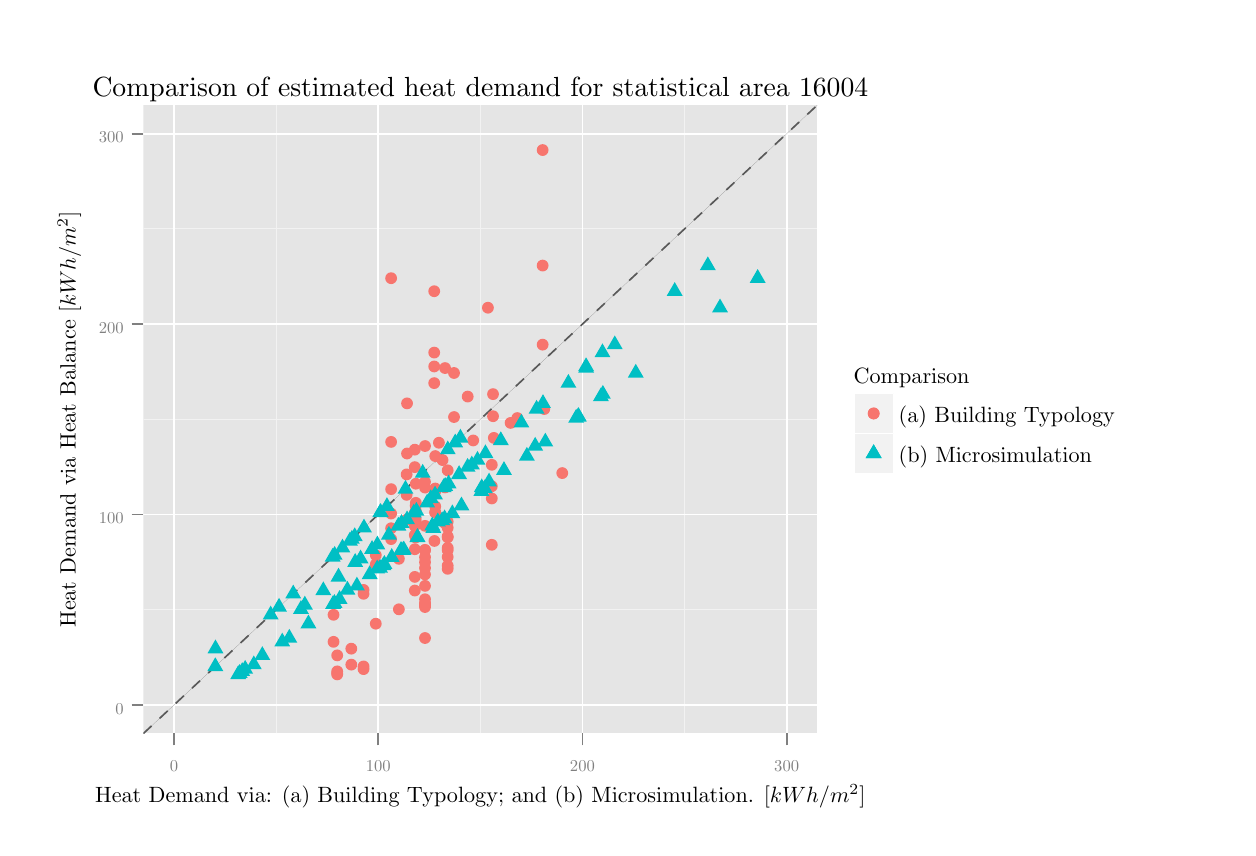
\begin{tikzpicture}[x=1pt,y=1pt]
\definecolor[named]{fillColor}{rgb}{1.00,1.00,1.00}
\path[use as bounding box,fill=fillColor,fill opacity=0.00] (0,0) rectangle (433.62,289.08);
\begin{scope}
\path[clip] (  0.00,  0.00) rectangle (433.62,289.08);
\definecolor[named]{drawColor}{rgb}{1.00,1.00,1.00}
\definecolor[named]{fillColor}{rgb}{1.00,1.00,1.00}

\path[draw=drawColor,line width= 0.6pt,line join=round,line cap=round,fill=fillColor] ( -0.00,  0.00) rectangle (433.62,289.08);
\end{scope}
\begin{scope}
\path[clip] ( 41.82, 34.03) rectangle (285.33,261.09);
\definecolor[named]{fillColor}{rgb}{0.90,0.90,0.90}

\path[fill=fillColor] ( 41.82, 34.03) rectangle (285.33,261.09);
\definecolor[named]{drawColor}{rgb}{0.95,0.95,0.95}

\path[draw=drawColor,line width= 0.3pt,line join=round] ( 41.82, 78.76) --
	(285.33, 78.76);

\path[draw=drawColor,line width= 0.3pt,line join=round] ( 41.82,147.56) --
	(285.33,147.56);

\path[draw=drawColor,line width= 0.3pt,line join=round] ( 41.82,216.37) --
	(285.33,216.37);

\path[draw=drawColor,line width= 0.3pt,line join=round] ( 89.78, 34.03) --
	( 89.78,261.09);

\path[draw=drawColor,line width= 0.3pt,line join=round] (163.58, 34.03) --
	(163.58,261.09);

\path[draw=drawColor,line width= 0.3pt,line join=round] (237.37, 34.03) --
	(237.37,261.09);
\definecolor[named]{drawColor}{rgb}{1.00,1.00,1.00}

\path[draw=drawColor,line width= 0.6pt,line join=round] ( 41.82, 44.36) --
	(285.33, 44.36);

\path[draw=drawColor,line width= 0.6pt,line join=round] ( 41.82,113.16) --
	(285.33,113.16);

\path[draw=drawColor,line width= 0.6pt,line join=round] ( 41.82,181.97) --
	(285.33,181.97);

\path[draw=drawColor,line width= 0.6pt,line join=round] ( 41.82,250.77) --
	(285.33,250.77);

\path[draw=drawColor,line width= 0.6pt,line join=round] ( 52.89, 34.03) --
	( 52.89,261.09);

\path[draw=drawColor,line width= 0.6pt,line join=round] (126.68, 34.03) --
	(126.68,261.09);

\path[draw=drawColor,line width= 0.6pt,line join=round] (200.47, 34.03) --
	(200.47,261.09);

\path[draw=drawColor,line width= 0.6pt,line join=round] (274.26, 34.03) --
	(274.26,261.09);
\definecolor[named]{drawColor}{rgb}{0.35,0.35,0.35}
\definecolor[named]{fillColor}{rgb}{0.35,0.35,0.35}

\path[draw=drawColor,line width= 0.6pt,dash pattern=on 4pt off 4pt ,line join=round,fill=fillColor] ( 41.82, 34.03) -- (285.33,261.09);
\definecolor[named]{fillColor}{rgb}{0.97,0.46,0.43}

\path[fill=fillColor] (131.33,139.40) circle (  2.13);

\path[fill=fillColor] (139.89, 90.61) circle (  2.13);

\path[fill=fillColor] (147.27,121.57) circle (  2.13);

\path[fill=fillColor] (134.13, 78.91) circle (  2.13);

\path[fill=fillColor] (186.08,244.86) circle (  2.13);

\path[fill=fillColor] (131.33,108.20) circle (  2.13);

\path[fill=fillColor] (159.00,155.78) circle (  2.13);

\path[fill=fillColor] (167.71,131.12) circle (  2.13);

\path[fill=fillColor] (147.27,116.09) circle (  2.13);

\path[fill=fillColor] (140.26,124.28) circle (  2.13);

\path[fill=fillColor] (154.06,164.30) circle (  2.13);

\path[fill=fillColor] (150.81,110.00) circle (  2.13);

\path[fill=fillColor] (143.58, 95.91) circle (  2.13);

\path[fill=fillColor] (168.15,148.68) circle (  2.13);

\path[fill=fillColor] (140.18,111.66) circle (  2.13);

\path[fill=fillColor] (136.94,127.65) circle (  2.13);

\path[fill=fillColor] (154.06,148.38) circle (  2.13);

\path[fill=fillColor] (168.45,140.84) circle (  2.13);

\path[fill=fillColor] (160.99,139.92) circle (  2.13);

\path[fill=fillColor] (143.58,100.21) circle (  2.13);

\path[fill=fillColor] (167.71,118.96) circle (  2.13);

\path[fill=fillColor] (111.85, 56.48) circle (  2.13);

\path[fill=fillColor] (166.31,187.88) circle (  2.13);

\path[fill=fillColor] (151.77,101.10) circle (  2.13);

\path[fill=fillColor] (147.27,122.55) circle (  2.13);

\path[fill=fillColor] (121.37, 85.91) circle (  2.13);

\path[fill=fillColor] (151.77,110.57) circle (  2.13);

\path[fill=fillColor] (143.58,122.88) circle (  2.13);

\path[fill=fillColor] (151.77,108.35) circle (  2.13);

\path[fill=fillColor] (136.94,111.31) circle (  2.13);

\path[fill=fillColor] (139.89,109.03) circle (  2.13);

\path[fill=fillColor] (167.71,102.21) circle (  2.13);

\path[fill=fillColor] (151.77,105.23) circle (  2.13);

\path[fill=fillColor] (174.50,146.26) circle (  2.13);

\path[fill=fillColor] (125.79, 98.47) circle (  2.13);

\path[fill=fillColor] (143.58, 81.10) circle (  2.13);

\path[fill=fillColor] (111.85, 55.38) circle (  2.13);

\path[fill=fillColor] (143.58, 82.54) circle (  2.13);

\path[fill=fillColor] (140.18,110.98) circle (  2.13);

\path[fill=fillColor] (150.81,122.94) circle (  2.13);

\path[fill=fillColor] (131.33,113.51) circle (  2.13);

\path[fill=fillColor] (139.89,113.74) circle (  2.13);

\path[fill=fillColor] (143.58, 80.49) circle (  2.13);

\path[fill=fillColor] (110.52, 76.92) circle (  2.13);

\path[fill=fillColor] (131.33,122.33) circle (  2.13);

\path[fill=fillColor] (151.77,129.13) circle (  2.13);

\path[fill=fillColor] (125.79, 95.18) circle (  2.13);

\path[fill=fillColor] (143.58, 80.73) circle (  2.13);

\path[fill=fillColor] (186.08,203.12) circle (  2.13);

\path[fill=fillColor] (146.90,193.84) circle (  2.13);

\path[fill=fillColor] (176.93,148.01) circle (  2.13);

\path[fill=fillColor] (121.37, 57.30) circle (  2.13);

\path[fill=fillColor] (143.58,124.96) circle (  2.13);

\path[fill=fillColor] (134.13, 97.15) circle (  2.13);

\path[fill=fillColor] (143.58,100.39) circle (  2.13);

\path[fill=fillColor] (147.27,134.27) circle (  2.13);

\path[fill=fillColor] (139.89, 85.69) circle (  2.13);

\path[fill=fillColor] (151.77, 94.68) circle (  2.13);

\path[fill=fillColor] (148.60,139.09) circle (  2.13);

\path[fill=fillColor] (140.18,104.84) circle (  2.13);

\path[fill=fillColor] (139.89,136.59) circle (  2.13);

\path[fill=fillColor] (111.85, 55.82) circle (  2.13);

\path[fill=fillColor] (116.94, 64.68) circle (  2.13);

\path[fill=fillColor] (186.67,151.27) circle (  2.13);

\path[fill=fillColor] (167.71,123.37) circle (  2.13);

\path[fill=fillColor] (147.27,113.83) circle (  2.13);

\path[fill=fillColor] (143.58, 91.51) circle (  2.13);

\path[fill=fillColor] (131.33,198.55) circle (  2.13);

\path[fill=fillColor] (193.17,128.13) circle (  2.13);

\path[fill=fillColor] (121.37, 84.51) circle (  2.13);

\path[fill=fillColor] (140.26,114.40) circle (  2.13);

\path[fill=fillColor] (139.89,100.61) circle (  2.13);

\path[fill=fillColor] (125.79, 73.70) circle (  2.13);

\path[fill=fillColor] (111.85, 62.26) circle (  2.13);

\path[fill=fillColor] (136.94,120.26) circle (  2.13);

\path[fill=fillColor] (150.81,166.08) circle (  2.13);

\path[fill=fillColor] (140.18,116.34) circle (  2.13);

\path[fill=fillColor] (131.33,104.27) circle (  2.13);

\path[fill=fillColor] (143.58, 93.81) circle (  2.13);

\path[fill=fillColor] (139.89,105.76) circle (  2.13);

\path[fill=fillColor] (139.89,130.28) circle (  2.13);

\path[fill=fillColor] (149.92,132.83) circle (  2.13);

\path[fill=fillColor] (110.52, 67.15) circle (  2.13);

\path[fill=fillColor] (151.77, 93.54) circle (  2.13);

\path[fill=fillColor] (137.08,135.20) circle (  2.13);

\path[fill=fillColor] (121.37, 58.26) circle (  2.13);

\path[fill=fillColor] (137.08,153.32) circle (  2.13);

\path[fill=fillColor] (116.94, 58.91) circle (  2.13);

\path[fill=fillColor] (143.58,137.90) circle (  2.13);

\path[fill=fillColor] (143.58, 87.37) circle (  2.13);

\path[fill=fillColor] (146.90,171.67) circle (  2.13);

\path[fill=fillColor] (168.15,156.66) circle (  2.13);

\path[fill=fillColor] (186.08,174.54) circle (  2.13);

\path[fill=fillColor] (143.58, 68.53) circle (  2.13);

\path[fill=fillColor] (151.77,104.90) circle (  2.13);

\path[fill=fillColor] (140.26,117.37) circle (  2.13);

\path[fill=fillColor] (147.27,113.98) circle (  2.13);

\path[fill=fillColor] (146.97,103.60) circle (  2.13);

\path[fill=fillColor] (143.58,109.06) circle (  2.13);

\path[fill=fillColor] (146.90,160.64) circle (  2.13);

\path[fill=fillColor] (151.77,100.26) circle (  2.13);

\path[fill=fillColor] (151.77, 97.81) circle (  2.13);

\path[fill=fillColor] (143.58, 79.73) circle (  2.13);

\path[fill=fillColor] (143.58, 97.71) circle (  2.13);

\path[fill=fillColor] (146.90,166.65) circle (  2.13);
\definecolor[named]{fillColor}{rgb}{0.00,0.75,0.77}

\path[fill=fillColor] (187.05,142.72) --
	(189.92,137.74) --
	(184.17,137.74) --
	cycle;

\path[fill=fillColor] (112.33, 93.93) --
	(115.20, 88.95) --
	(109.46, 88.95) --
	cycle;

\path[fill=fillColor] (163.94,124.88) --
	(166.82,119.91) --
	(161.07,119.91) --
	cycle;

\path[fill=fillColor] ( 98.74, 82.23) --
	(101.61, 77.25) --
	( 95.87, 77.25) --
	cycle;

\path[fill=fillColor] (146.56,111.52) --
	(149.44,106.54) --
	(143.69,106.54) --
	cycle;

\path[fill=fillColor] (207.14,159.10) --
	(210.01,154.12) --
	(204.26,154.12) --
	cycle;

\path[fill=fillColor] (160.49,134.44) --
	(163.37,129.46) --
	(157.62,129.46) --
	cycle;

\path[fill=fillColor] (129.82,119.41) --
	(132.70,114.43) --
	(126.95,114.43) --
	cycle;

\path[fill=fillColor] (152.09,127.60) --
	(154.97,122.62) --
	(149.22,122.62) --
	cycle;

\path[fill=fillColor] (219.73,167.62) --
	(222.60,162.64) --
	(216.86,162.64) --
	cycle;

\path[fill=fillColor] (135.08,113.32) --
	(137.96,108.34) --
	(132.21,108.34) --
	cycle;

\path[fill=fillColor] (118.34, 99.23) --
	(121.22, 94.25) --
	(115.47, 94.25) --
	cycle;

\path[fill=fillColor] (198.97,151.99) --
	(201.85,147.02) --
	(196.10,147.02) --
	cycle;

\path[fill=fillColor] (150.66,114.98) --
	(153.53,110.00) --
	(147.78,110.00) --
	cycle;

\path[fill=fillColor] (155.89,130.97) --
	(158.76,125.99) --
	(153.01,125.99) --
	cycle;

\path[fill=fillColor] (199.13,151.70) --
	(202.01,146.72) --
	(196.26,146.72) --
	cycle;

\path[fill=fillColor] (156.36,144.16) --
	(159.24,139.18) --
	(153.49,139.18) --
	cycle;

\path[fill=fillColor] (170.96,143.24) --
	(173.84,138.26) --
	(168.09,138.26) --
	cycle;

\path[fill=fillColor] (135.69,103.53) --
	(138.56, 98.55) --
	(132.81, 98.55) --
	cycle;

\path[fill=fillColor] (145.66,122.28) --
	(148.54,117.30) --
	(142.79,117.30) --
	cycle;

\path[fill=fillColor] ( 77.52, 59.80) --
	( 80.39, 54.82) --
	( 74.65, 54.82) --
	cycle;

\path[fill=fillColor] (250.18,191.20) --
	(253.05,186.22) --
	(247.31,186.22) --
	cycle;

\path[fill=fillColor] (113.75,104.42) --
	(116.62, 99.44) --
	(110.87, 99.44) --
	cycle;

\path[fill=fillColor] (165.19,125.87) --
	(168.06,120.89) --
	(162.32,120.89) --
	cycle;

\path[fill=fillColor] (115.54, 89.22) --
	(118.41, 84.25) --
	(112.66, 84.25) --
	cycle;

\path[fill=fillColor] (148.20,113.89) --
	(151.08,108.91) --
	(145.33,108.91) --
	cycle;

\path[fill=fillColor] (164.07,126.20) --
	(166.95,121.22) --
	(161.20,121.22) --
	cycle;

\path[fill=fillColor] (121.52,111.67) --
	(124.40,106.69) --
	(118.65,106.69) --
	cycle;

\path[fill=fillColor] (137.09,114.63) --
	(139.96,109.65) --
	(134.22,109.65) --
	cycle;

\path[fill=fillColor] (133.96,112.35) --
	(136.84,107.37) --
	(131.09,107.37) --
	cycle;

\path[fill=fillColor] (126.37,105.53) --
	(129.24,100.55) --
	(123.50,100.55) --
	cycle;

\path[fill=fillColor] (118.18,108.55) --
	(121.05,103.57) --
	(115.30,103.57) --
	cycle;

\path[fill=fillColor] (178.41,149.58) --
	(181.28,144.61) --
	(175.53,144.61) --
	cycle;

\path[fill=fillColor] (110.93,101.79) --
	(113.80, 96.82) --
	(108.06, 96.82) --
	cycle;

\path[fill=fillColor] (110.88, 84.41) --
	(113.75, 79.44) --
	(108.00, 79.44) --
	cycle;

\path[fill=fillColor] ( 76.08, 58.70) --
	( 78.95, 53.72) --
	( 73.21, 53.72) --
	cycle;

\path[fill=fillColor] (112.70, 85.86) --
	(115.57, 80.88) --
	(109.83, 80.88) --
	cycle;

\path[fill=fillColor] (149.77,114.30) --
	(152.65,109.32) --
	(146.90,109.32) --
	cycle;

\path[fill=fillColor] (150.32,126.26) --
	(153.19,121.28) --
	(147.44,121.28) --
	cycle;

\path[fill=fillColor] (153.46,116.83) --
	(156.33,111.85) --
	(150.59,111.85) --
	cycle;

\path[fill=fillColor] (139.52,117.05) --
	(142.40,112.08) --
	(136.65,112.08) --
	cycle;

\path[fill=fillColor] (100.15, 83.81) --
	(103.03, 78.83) --
	( 97.28, 78.83) --
	cycle;

\path[fill=fillColor] ( 87.81, 80.24) --
	( 90.68, 75.26) --
	( 84.94, 75.26) --
	cycle;

\path[fill=fillColor] (136.51,125.65) --
	(139.39,120.67) --
	(133.64,120.67) --
	cycle;

\path[fill=fillColor] (172.11,132.45) --
	(174.99,127.47) --
	(169.24,127.47) --
	cycle;

\path[fill=fillColor] (128.91, 98.50) --
	(131.79, 93.52) --
	(126.04, 93.52) --
	cycle;

\path[fill=fillColor] (110.35, 84.05) --
	(113.22, 79.07) --
	(107.48, 79.07) --
	cycle;

\path[fill=fillColor] (245.77,206.43) --
	(248.64,201.46) --
	(242.89,201.46) --
	cycle;

\path[fill=fillColor] (233.80,197.16) --
	(236.67,192.18) --
	(230.92,192.18) --
	cycle;

\path[fill=fillColor] (198.19,151.33) --
	(201.07,146.35) --
	(195.32,146.35) --
	cycle;

\path[fill=fillColor] ( 78.59, 60.61) --
	( 81.47, 55.64) --
	( 75.72, 55.64) --
	cycle;

\path[fill=fillColor] (166.72,128.28) --
	(169.59,123.30) --
	(163.85,123.30) --
	cycle;

\path[fill=fillColor] (120.29,100.47) --
	(123.17, 95.50) --
	(117.42, 95.50) --
	cycle;

\path[fill=fillColor] (135.92,103.71) --
	(138.80, 98.73) --
	(133.05, 98.73) --
	cycle;

\path[fill=fillColor] (180.38,137.59) --
	(183.26,132.61) --
	(177.51,132.61) --
	cycle;

\path[fill=fillColor] (106.83, 89.00) --
	(109.71, 84.03) --
	(103.96, 84.03) --
	cycle;

\path[fill=fillColor] (128.56, 98.00) --
	(131.44, 93.02) --
	(125.69, 93.02) --
	cycle;

\path[fill=fillColor] (154.49,142.41) --
	(157.36,137.43) --
	(151.62,137.43) --
	cycle;

\path[fill=fillColor] (140.84,108.16) --
	(143.71,103.18) --
	(137.97,103.18) --
	cycle;

\path[fill=fillColor] (151.81,139.91) --
	(154.68,134.94) --
	(148.94,134.94) --
	cycle;

\path[fill=fillColor] ( 76.60, 59.13) --
	( 79.47, 54.16) --
	( 73.73, 54.16) --
	cycle;

\path[fill=fillColor] ( 67.86, 68.00) --
	( 70.74, 63.02) --
	( 64.99, 63.02) --
	cycle;

\path[fill=fillColor] (183.89,154.59) --
	(186.76,149.61) --
	(181.01,149.61) --
	cycle;

\path[fill=fillColor] (150.86,126.69) --
	(153.73,121.71) --
	(147.98,121.71) --
	cycle;

\path[fill=fillColor] (127.39,117.14) --
	(130.27,112.17) --
	(124.52,112.17) --
	cycle;

\path[fill=fillColor] (123.60, 94.83) --
	(126.47, 89.85) --
	(120.72, 89.85) --
	cycle;

\path[fill=fillColor] (263.78,201.87) --
	(266.66,196.89) --
	(260.91,196.89) --
	cycle;

\path[fill=fillColor] (142.74,131.45) --
	(145.61,126.47) --
	(139.86,126.47) --
	cycle;

\path[fill=fillColor] ( 95.96, 87.83) --
	( 98.83, 82.85) --
	( 93.08, 82.85) --
	cycle;

\path[fill=fillColor] (140.47,117.72) --
	(143.35,112.74) --
	(137.60,112.74) --
	cycle;

\path[fill=fillColor] (124.44,103.93) --
	(127.32, 98.95) --
	(121.57, 98.95) --
	cycle;

\path[fill=fillColor] (101.45, 77.02) --
	(104.32, 72.04) --
	( 98.57, 72.04) --
	cycle;

\path[fill=fillColor] ( 84.79, 65.58) --
	( 87.66, 60.60) --
	( 81.92, 60.60) --
	cycle;

\path[fill=fillColor] (147.20,123.58) --
	(150.07,118.60) --
	(144.32,118.60) --
	cycle;

\path[fill=fillColor] (201.81,169.40) --
	(204.68,164.42) --
	(198.93,164.42) --
	cycle;

\path[fill=fillColor] (156.75,119.65) --
	(159.62,114.68) --
	(153.87,114.68) --
	cycle;

\path[fill=fillColor] (117.14,107.59) --
	(120.02,102.61) --
	(114.27,102.61) --
	cycle;

\path[fill=fillColor] (127.33, 97.13) --
	(130.20, 92.15) --
	(124.45, 92.15) --
	cycle;

\path[fill=fillColor] (130.53,109.08) --
	(133.40,104.10) --
	(127.65,104.10) --
	cycle;

\path[fill=fillColor] (158.97,133.60) --
	(161.84,128.62) --
	(156.10,128.62) --
	cycle;

\path[fill=fillColor] (162.54,136.14) --
	(165.41,131.17) --
	(159.67,131.17) --
	cycle;

\path[fill=fillColor] ( 91.99, 70.47) --
	( 94.87, 65.49) --
	( 89.12, 65.49) --
	cycle;

\path[fill=fillColor] (126.29, 96.86) --
	(129.17, 91.88) --
	(123.42, 91.88) --
	cycle;

\path[fill=fillColor] (165.41,138.51) --
	(168.29,133.54) --
	(162.54,133.54) --
	cycle;

\path[fill=fillColor] ( 67.80, 61.58) --
	( 70.68, 56.60) --
	( 64.93, 56.60) --
	cycle;

\path[fill=fillColor] (186.21,156.64) --
	(189.08,151.66) --
	(183.34,151.66) --
	cycle;

\path[fill=fillColor] ( 81.71, 62.23) --
	( 84.59, 57.25) --
	( 78.84, 57.25) --
	cycle;

\path[fill=fillColor] (183.39,141.22) --
	(186.26,136.24) --
	(180.51,136.24) --
	cycle;

\path[fill=fillColor] (118.97, 90.69) --
	(121.85, 85.71) --
	(116.10, 85.71) --
	cycle;

\path[fill=fillColor] (207.69,174.99) --
	(210.56,170.01) --
	(204.82,170.01) --
	cycle;

\path[fill=fillColor] (207.85,159.98) --
	(210.72,155.00) --
	(204.97,155.00) --
	cycle;

\path[fill=fillColor] (212.15,177.86) --
	(215.02,172.89) --
	(209.27,172.89) --
	cycle;

\path[fill=fillColor] ( 94.55, 71.84) --
	( 97.42, 66.87) --
	( 91.68, 66.87) --
	cycle;

\path[fill=fillColor] (140.86,108.22) --
	(143.73,103.24) --
	(137.98,103.24) --
	cycle;

\path[fill=fillColor] (144.35,120.68) --
	(147.23,115.71) --
	(141.48,115.71) --
	cycle;

\path[fill=fillColor] (127.55,117.29) --
	(130.43,112.32) --
	(124.68,112.32) --
	cycle;

\path[fill=fillColor] (116.42,106.92) --
	(119.30,101.94) --
	(113.55,101.94) --
	cycle;

\path[fill=fillColor] (146.21,112.38) --
	(149.09,107.40) --
	(143.34,107.40) --
	cycle;

\path[fill=fillColor] (195.39,163.96) --
	(198.27,158.98) --
	(192.52,158.98) --
	cycle;

\path[fill=fillColor] (134.92,103.58) --
	(137.79, 98.60) --
	(132.05, 98.60) --
	cycle;

\path[fill=fillColor] (110.21,101.13) --
	(113.09, 96.15) --
	(107.34, 96.15) --
	cycle;

\path[fill=fillColor] ( 90.83, 83.05) --
	( 93.70, 78.08) --
	( 87.96, 78.08) --
	cycle;

\path[fill=fillColor] (131.55,101.03) --
	(134.42, 96.05) --
	(128.68, 96.05) --
	cycle;

\path[fill=fillColor] (201.78,169.97) --
	(204.65,164.99) --
	(198.91,164.99) --
	cycle;
\end{scope}
\begin{scope}
\path[clip] (  0.00,  0.00) rectangle (433.62,289.08);
\definecolor[named]{drawColor}{rgb}{0.50,0.50,0.50}

\node[text=drawColor,anchor=base east,inner sep=0pt, outer sep=0pt, scale= 0.6]
at ( 34.71, 41.05) {0};

\node[text=drawColor,anchor=base east,inner sep=0pt, outer sep=0pt, scale=  0.6] at ( 34.71,109.86) {100};

\node[text=drawColor,anchor=base east,inner sep=0pt, outer sep=0pt, scale=  0.6] at ( 34.71,178.66) {200};

\node[text=drawColor,anchor=base east,inner sep=0pt, outer sep=0pt, scale=  0.6] at ( 34.71,247.47) {300};
\end{scope}
\begin{scope}
\path[clip] (  0.00,  0.00) rectangle (433.62,289.08);
\definecolor[named]{drawColor}{rgb}{0.50,0.50,0.50}

\path[draw=drawColor,line width= 0.6pt,line join=round] ( 37.55, 44.36) --
	( 41.82, 44.36);

\path[draw=drawColor,line width= 0.6pt,line join=round] ( 37.55,113.16) --
	( 41.82,113.16);

\path[draw=drawColor,line width= 0.6pt,line join=round] ( 37.55,181.97) --
	( 41.82,181.97);

\path[draw=drawColor,line width= 0.6pt,line join=round] ( 37.55,250.77) --
	( 41.82,250.77);
\end{scope}
\begin{scope}
\path[clip] (  0.00,  0.00) rectangle (433.62,289.08);
\definecolor[named]{drawColor}{rgb}{0.50,0.50,0.50}

\path[draw=drawColor,line width= 0.6pt,line join=round] ( 52.89, 29.77) --
	( 52.89, 34.03);

\path[draw=drawColor,line width= 0.6pt,line join=round] (126.68, 29.77) --
	(126.68, 34.03);

\path[draw=drawColor,line width= 0.6pt,line join=round] (200.47, 29.77) --
	(200.47, 34.03);

\path[draw=drawColor,line width= 0.6pt,line join=round] (274.26, 29.77) --
	(274.26, 34.03);
\end{scope}
\begin{scope}
\path[clip] (  0.00,  0.00) rectangle (433.62,289.08);
\definecolor[named]{drawColor}{rgb}{0.50,0.50,0.50}

\node[text=drawColor,anchor=base,inner sep=0pt, outer sep=0pt, scale= 0.6] at (
52.89, 20.31) {0};

\node[text=drawColor,anchor=base,inner sep=0pt, outer sep=0pt, scale=  0.6] at (126.68, 20.31) {100};

\node[text=drawColor,anchor=base,inner sep=0pt, outer sep=0pt, scale=  0.6] at (200.47, 20.31) {200};

\node[text=drawColor,anchor=base,inner sep=0pt, outer sep=0pt, scale=  0.6] at (274.26, 20.31) {300};
\end{scope}
\begin{scope}
\path[clip] (  0.00,  0.00) rectangle (433.62,289.08);
\definecolor[named]{drawColor}{rgb}{0.00,0.00,0.00}

\node[text=drawColor,anchor=base,inner sep=0pt, outer sep=0pt, scale= 0.8] at
(163.58,  9.03) {Heat Demand via: (a) Building Typology; and (b) Microsimulation. $[kWh/m^2]$};
\end{scope}
\begin{scope}
\path[clip] (  0.00,  0.00) rectangle (433.62,289.08);
\definecolor[named]{drawColor}{rgb}{0.00,0.00,0.00}

\node[text=drawColor,rotate= 90.00,anchor=base,inner sep=0pt, outer sep=0pt,
scale= 0.8] at ( 17.30,147.56) {Heat Demand via Heat Balance $[kWh/m^2]$};
\end{scope}
\begin{scope}
\path[clip] (  0.00,  0.00) rectangle (433.62,289.08);
\definecolor[named]{fillColor}{rgb}{1.00,1.00,1.00}

\path[fill=fillColor] (294.20,123.72) rectangle (412.71,171.41);
\end{scope}
\begin{scope}
\path[clip] (  0.00,  0.00) rectangle (433.62,289.08);
\definecolor[named]{drawColor}{rgb}{0.00,0.00,0.00}

\node[text=drawColor,anchor=base west,inner sep=0pt, outer sep=0pt, scale= 
0.8] at (298.47,160.51) {Comparison};
\end{scope}
\begin{scope}
\path[clip] (  0.00,  0.00) rectangle (433.62,289.08);
\definecolor[named]{drawColor}{rgb}{1.00,1.00,1.00}
\definecolor[named]{fillColor}{rgb}{0.95,0.95,0.95}

\path[draw=drawColor,line width= 0.6pt,line join=round,line
cap=round,fill=fillColor] (298.47,142.45) rectangle (312.92,156.90);
\end{scope}
\begin{scope}
\path[clip] (  0.00,  0.00) rectangle (433.62,289.08);
\definecolor[named]{fillColor}{rgb}{0.97,0.46,0.43}

\path[fill=fillColor] (305.69,149.67) circle (  2.13);
\end{scope}
\begin{scope}
\path[clip] (  0.00,  0.00) rectangle (433.62,289.08);
\definecolor[named]{fillColor}{rgb}{0.97,0.46,0.43}

\path[fill=fillColor] (305.69,149.67) circle (  2.13);
\end{scope}
\begin{scope}
\path[clip] (  0.00,  0.00) rectangle (433.62,289.08);
\definecolor[named]{drawColor}{rgb}{1.00,1.00,1.00}
\definecolor[named]{fillColor}{rgb}{0.95,0.95,0.95}

\path[draw=drawColor,line width= 0.6pt,line join=round,line
cap=round,fill=fillColor] (298.47,127.99) rectangle (312.92,142.45);
\end{scope}
\begin{scope}
\path[clip] (  0.00,  0.00) rectangle (433.62,289.08);
\definecolor[named]{fillColor}{rgb}{0.00,0.75,0.77}

\path[fill=fillColor] (305.69,138.54) --
	(308.57,133.56) --
	(302.82,133.56) --
	cycle;
\end{scope}
\begin{scope}
\path[clip] (  0.00,  0.00) rectangle (433.62,289.08);
\definecolor[named]{fillColor}{rgb}{0.00,0.75,0.77}

\path[fill=fillColor] (305.69,138.54) --
	(308.57,133.56) --
	(302.82,133.56) --
	cycle;
\end{scope}
\begin{scope}
\path[clip] (  0.00,  0.00) rectangle (433.62,289.08);
\definecolor[named]{drawColor}{rgb}{0.00,0.00,0.00}

\node[text=drawColor,anchor=base west,inner sep=0pt, outer sep=0pt, scale= 
0.8] at (314.73,146.37) {(a) Building Typology};
\end{scope}
\begin{scope}
\path[clip] (  0.00,  0.00) rectangle (433.62,289.08);
\definecolor[named]{drawColor}{rgb}{0.00,0.00,0.00}

\node[text=drawColor,anchor=base west,inner sep=0pt, outer sep=0pt, scale= 
0.8] at (314.73,131.91) {(b) Microsimulation};
\end{scope}
\begin{scope}
\path[clip] (  0.00,  0.00) rectangle (433.62,289.08);
\definecolor[named]{drawColor}{rgb}{0.00,0.00,0.00}

\node[text=drawColor,anchor=base,inner sep=0pt, outer sep=0pt, scale= 1] at
(163.58,264.11) {Comparison of estimated heat demand for statistical area 16004};
\end{scope}
\end{tikzpicture}
\label{fig:7}
    \begin{flushleft}
    \begin{footnotesize}
        Comparison between heat demand estimated with a heat balance method,
        using the ``average'' occupant (vertical axis) and with help of: (a)
        building typologies; and (b) a heat balance, taking into account
        occupant influence, induce thought the synthetic simulated demographic
        characteristics via a spatial microsimulation (horizontal axis). This
        comparison shows the results of buildings in statistical area 16004
    \end{footnotesize}
    \end{flushleft}
\end{figure}

We present the result for the selected statistical area (16004) by comparing:
(1) the estimated heat demand with help of the ``standard'' heat balance model,
this model assumes an ``average'' household and so makes uses of the standard
internal gains, internal temperature and ventilation rates, corresponding to
row 3 of Table~\ref{tab:5} and (2) the implementation of the heat balance
method, varying input parameters ($qi$, $Ti$ and $n$) as a function of the
computed average working hours of the building, thus simulating heat
consumption. The result of this comparison in presented in Figure~\ref{fig:7}.
One can clearly see in the plot that the simulated heat consumption shows a
bigger spread. This is plausible, as it considers a richer spectrum of occupant
types. The analyzed statistical area still has a high proportion of ``old''
buildings, that is buildings predating the first (WSVO) Heat conservation
ordinance in 1977 (see Figure~\ref{fig:8}). We can expect a much higher
relative spread in urban areas that have been recently developed or
re-developed (``relative'' meaning: relative in terms of the overall amount of
heat consumption).

On average the simulated heat consumption is much higher than the estimated
heat demand. The selected urban area does not represent the average household
in Hamburg.  Table~\ref{tab:6} compares some attributes with the average value
for the entire city. The selected area has: (1) a high level of unemployment,
which in our model means less or 0 working hours; (2) a lower share of single
person households, which raises the probability of having a resident with zero
working hours; and (3) a high share of households with children, leading also
to low working hours of the household.

\begin{figure}[htb] 
    \centering 
    \caption{Histogram showing the frequency of construction year in
    statistical area 16004.}\label{fig:8} 
    % Created by tikzDevice version 0.6.2-92-0ad2792 on 2013-12-01 00:58:43
% !TEX encoding = UTF-8 Unicode
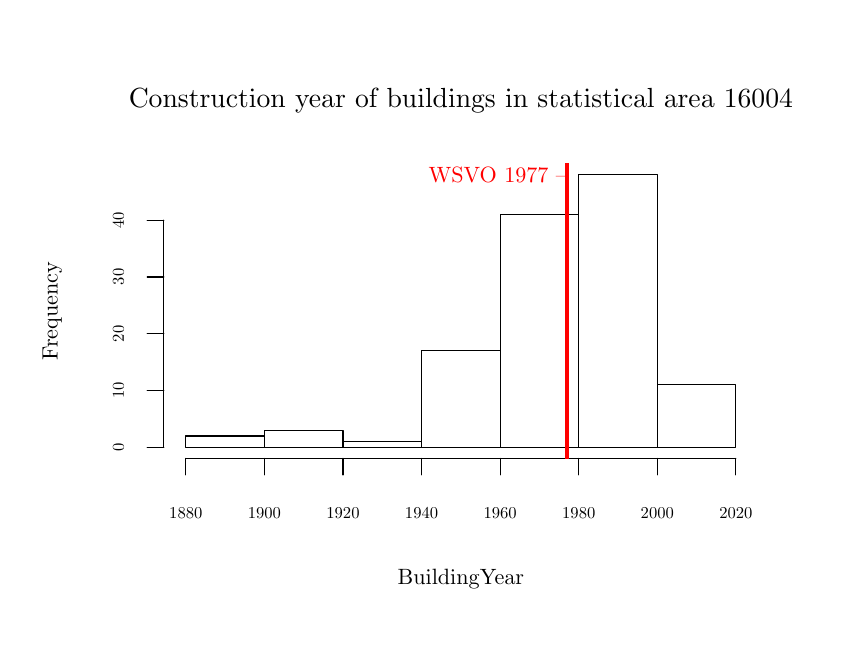
\begin{tikzpicture}[x=1pt,y=1pt]
\definecolor[named]{fillColor}{rgb}{1.00,1.00,1.00}
\path[use as bounding box,fill=fillColor,fill opacity=0.00] (0,0) rectangle (289.08,216.81);
\begin{scope}
\path[clip] (  0.00,  0.00) rectangle (289.08,216.81);
\definecolor[named]{drawColor}{rgb}{0.00,0.00,0.00}

\node[text=drawColor,anchor=base,inner sep=0pt, outer sep=0pt, scale=  1.0] at
(156.54,188.07) {Construction year of buildings in statistical area 16004};

\node[text=drawColor,anchor=base,inner sep=0pt, outer sep=0pt, scale=  0.8] at (156.54, 15.60) {BuildingYear};

\node[text=drawColor,rotate= 90.00,anchor=base,inner sep=0pt, outer sep=0pt,
scale=  0.8] at ( 10.80,114.41) {Frequency};
\end{scope}
\begin{scope}
\path[clip] (  0.00,  0.00) rectangle (289.08,216.81);
\definecolor[named]{drawColor}{rgb}{0.00,0.00,0.00}

\path[draw=drawColor,line width= 0.4pt,line join=round,line cap=round] ( 57.15, 61.20) -- (255.93, 61.20);

\path[draw=drawColor,line width= 0.4pt,line join=round,line cap=round] ( 57.15, 61.20) -- ( 57.15, 55.20);

\path[draw=drawColor,line width= 0.4pt,line join=round,line cap=round] ( 85.55, 61.20) -- ( 85.55, 55.20);

\path[draw=drawColor,line width= 0.4pt,line join=round,line cap=round] (113.94, 61.20) -- (113.94, 55.20);

\path[draw=drawColor,line width= 0.4pt,line join=round,line cap=round] (142.34, 61.20) -- (142.34, 55.20);

\path[draw=drawColor,line width= 0.4pt,line join=round,line cap=round] (170.74, 61.20) -- (170.74, 55.20);

\path[draw=drawColor,line width= 0.4pt,line join=round,line cap=round] (199.14, 61.20) -- (199.14, 55.20);

\path[draw=drawColor,line width= 0.4pt,line join=round,line cap=round] (227.53, 61.20) -- (227.53, 55.20);

\path[draw=drawColor,line width= 0.4pt,line join=round,line cap=round] (255.93, 61.20) -- (255.93, 55.20);

\node[text=drawColor,anchor=base,inner sep=0pt, outer sep=0pt, scale=  0.6] at ( 57.15, 39.60) {1880};

\node[text=drawColor,anchor=base,inner sep=0pt, outer sep=0pt, scale=  0.6] at ( 85.55, 39.60) {1900};

\node[text=drawColor,anchor=base,inner sep=0pt, outer sep=0pt, scale=  0.6] at (113.94, 39.60) {1920};

\node[text=drawColor,anchor=base,inner sep=0pt, outer sep=0pt, scale=  0.6] at (142.34, 39.60) {1940};

\node[text=drawColor,anchor=base,inner sep=0pt, outer sep=0pt, scale=  0.6] at (170.74, 39.60) {1960};

\node[text=drawColor,anchor=base,inner sep=0pt, outer sep=0pt, scale=  0.6] at (199.14, 39.60) {1980};

\node[text=drawColor,anchor=base,inner sep=0pt, outer sep=0pt, scale=  0.6] at (227.53, 39.60) {2000};

\node[text=drawColor,anchor=base,inner sep=0pt, outer sep=0pt, scale=  0.6] at (255.93, 39.60) {2020};

\path[draw=drawColor,line width= 0.4pt,line join=round,line cap=round] ( 49.20, 65.14) -- ( 49.20,147.25);

\path[draw=drawColor,line width= 0.4pt,line join=round,line cap=round] ( 49.20, 65.14) -- ( 43.20, 65.14);

\path[draw=drawColor,line width= 0.4pt,line join=round,line cap=round] ( 49.20, 85.67) -- ( 43.20, 85.67);

\path[draw=drawColor,line width= 0.4pt,line join=round,line cap=round] ( 49.20,106.19) -- ( 43.20,106.19);

\path[draw=drawColor,line width= 0.4pt,line join=round,line cap=round] ( 49.20,126.72) -- ( 43.20,126.72);

\path[draw=drawColor,line width= 0.4pt,line join=round,line cap=round] ( 49.20,147.25) -- ( 43.20,147.25);

\node[text=drawColor,rotate= 90.00,anchor=base,inner sep=0pt, outer sep=0pt,
scale=  0.6] at ( 34.80, 65.14) {0};

\node[text=drawColor,rotate= 90.00,anchor=base,inner sep=0pt, outer sep=0pt,
scale=  0.6] at ( 34.80, 85.67) {10};

\node[text=drawColor,rotate= 90.00,anchor=base,inner sep=0pt, outer sep=0pt, scale=  0.6] at ( 34.80,106.19) {20};

\node[text=drawColor,rotate= 90.00,anchor=base,inner sep=0pt, outer sep=0pt, scale=  0.6] at ( 34.80,126.72) {30};

\node[text=drawColor,rotate= 90.00,anchor=base,inner sep=0pt, outer sep=0pt, scale=  0.6] at ( 34.80,147.25) {40};
\end{scope}
\begin{scope}
\path[clip] ( 49.20, 61.20) rectangle (263.88,167.61);
\definecolor[named]{drawColor}{rgb}{0.00,0.00,0.00}

\path[draw=drawColor,line width= 0.4pt,line join=round,line cap=round] ( 57.15, 65.14) rectangle ( 85.55, 69.25);

\path[draw=drawColor,line width= 0.4pt,line join=round,line cap=round] ( 85.55, 65.14) rectangle (113.94, 71.30);

\path[draw=drawColor,line width= 0.4pt,line join=round,line cap=round] (113.94, 65.14) rectangle (142.34, 67.19);

\path[draw=drawColor,line width= 0.4pt,line join=round,line cap=round] (142.34, 65.14) rectangle (170.74,100.04);

\path[draw=drawColor,line width= 0.4pt,line join=round,line cap=round] (170.74, 65.14) rectangle (199.14,149.30);

\path[draw=drawColor,line width= 0.4pt,line join=round,line cap=round] (199.14, 65.14) rectangle (227.53,163.67);

\path[draw=drawColor,line width= 0.4pt,line join=round,line cap=round] (227.53, 65.14) rectangle (255.93, 87.72);
\definecolor[named]{drawColor}{rgb}{1.00,0.00,0.00}

\path[draw=drawColor,line width= 1.6pt,line join=round,line cap=round] (194.88, 61.20) -- (194.88,167.61);

\node[text=drawColor,anchor=base east,inner sep=0pt, outer sep=0pt, scale=  0.8] at (194.88,160.89) {WSVO 1977 --};
\end{scope}
\end{tikzpicture}

    \begin{flushleft}
    \begin{footnotesize}
        To generate this distribution only known construction years are used
    \end{footnotesize}
    \end{flushleft}
\end{figure}

\begin{table}[htb]
    \centering 
    \caption{Description of some parameters of statistical area 16004 in
    comparison of the average value for the city of Hamburg}\label{tab:6}
    \begin{tabular}{lrrr}
        \addlinespace
        \toprule
        Statistical area 16004 & Hamburg & $\Delta$\\
        Size of household [\# individuals per household]&   2.0 &   1.8 &  0.2\\ 
        Share of foreign nationals [\%]                 &  45.1 &  13.6 & 31.5\\ 
        Share of household with kids [\%]               &  26.7 &  16.9 &  9.8\\ 
        Share of unemployed residents$^*$[\%]           &  12.2 &   4.8 &  7.4\\ 
        Share of single person households [\%]          &  49.8 &  51.2 &  1.4\\ 
        Number of private cars per 1000 residents [cars]& 180   & 353   &172  \\ 
        \bottomrule \addlinespace 
    \end{tabular} \\ 
    \begin{footnotesize}
    %    \begin{flushleft}
        $^*$ Residents between the ages of 15 and 65.
    %    \end{flushleft}
    \end{footnotesize}
\end{table}

\section{NEXT STEP:\@ INCLUDING A THERMAL SIMULATION MODEL}\label{sec:9}

In a further step we aim to integrate a thermal simulation model. This will
allow us to: (1) simulate at a much higher temporal resolution, needed for the
efficient dimensioning of decentralized energy supply systems; and (2) feed the
model with more detailed input data. The second reason is essential for
achieving our goal. Most of the defined energy balance norms or models take a
limited number of parameters as input; in particular there are few parameters
that are related to occupant behaviour. This is because the aim of the standard
method is the estimation of heat demand for the ``average'' occupant. Because
we want to represent the full spectrum of occupants and their corresponding
influence on the system we have to make use of a more flexible method for the
estimation of residential heat demand.  Because of the nature of the heat
accounting model, and the underlying national standard, we have to define a
range of occupant-related parameters for each dwelling unit, rather than a time
schedule reflecting occupants' presence. In our model we chose to estimate the
average working hours as we plan to extend the model to incorporate a thermal
simulation which is able to use a detailed occupants’ presence schedule as
input. This means that from variable ef147 onward (see Table~\ref{tab:4}) we
need to generate a detailed schedule for the simulation of heat consumption via
a thermal simulation \citeA{Widen.2011, Wilke.2011}  Another problem with the
use of a static heat balancing method is the inability of such a model to
integrate individual characteristics of dwelling units. The major problem by
attempting a dwelling-unit specific computation of heat consumption is the
required input variables regarding the building envelope. In order to perform a
dwelling unit based heat computation, we will have to define the geometry not
only of the building but of the dwelling unit itself, orientation, size of
facade, etc. This problem is no longer present for a proper thermal simulation
model as the generated schedule can define various levels of occupancy.

\section{Conclusions}\label{sec:10}

The presented results mark our first attempt to simulate heat consumption at an
urban scale, using microdata. Our model combines well established
implementations from: (a) the microsimulation community and (b) the building
simulation community. In this paper we have shown that a combination of both
methods is possible and can generate interesting insights into the planning of
cities and their technical infrastructures. We use a method from the
microsimulation community (the Hill Climbing algorithm) to select families from
the census database and allocate them into small statistical areas within the
city. From the digital cadaster we attribute the corresponding buildings with
energy relevant characteristics. In a third step we allocate the selected
families into individual buildings. The buildings with it inhabitants serve as
input data to a simplified heat balance model following the German DIN V 18599
standard.

We can show that the integration of socio-demographic characteristics of the
families living in a specific area can be used as input for the simulation of
heat consumption. This is an important contribution to both scientific
communities as: (a) it shows an interesting application of microsimulation in
the energy sector and (b) it presents an interesting approach for the building
simulation community to integrate the occupants of the buildings into the
simulation models not only within a sensitivity analysis but placing the
occupant central to the simulation.  Current models for projecting heat demand
employ an ``average'' occupant, both at a building scale and at an urban scale.
The trend towards decentralized, as well as more efficient technical systems
leads to greater sensitivity of technical systems. An integration of the
occupant into infrastructure models will play an important role in the future
of urban planning.

With our simplified model we have shown that we are able to indicate a
direction in the spread of estimated consumption that is plausible and
commensurate with what we know about the analyzed area to which it was applied.
As described in Section~\ref{sec:9}, we expect from future work --- integrating
a thermal simulation model and constructing a more accurate micro data set ---
promising results for the energy planning sector. Although this paper focuses
exclusively on heat energy, the range of questions that can be analyzed once a
population is allocated to buildings is manifold.

%%%%%%%%%%%%%%%%%%%%%%%%%%%%%%%%%%%%%%%%%%%%%%%%%
%%                  The Bibliography           %%
%%                                             %%              
%%  IJM-article.cls will be used to            %% 
%%  generate the bibliography                  %% 
%%                                             %%
%%%%%%%%%%%%%%%%%%%%%%%%%%%%%%%%%%%%%%%%%%%%%%%%%

\renewcommand{\refname}{REFERENCES}
\bibliographystyle{apacite}
%\bibliography{IJM-article}      % Bibliography file (usually '*.bib' ) 
\bibliography{IJM-MunozPeters}      % Bibliography file (usually '*.bib' ) 

%%%%%%%%%%%%%%%%%%%%%%%%%%%%%%%%%%%
%%                               %%
%% Figures                       %%
%%                               %%
%% NB: this is for captions and  %%
%% Titles. All graphics must be  %%
%% submitted separately and NOT  %%
%% included in the Tex document  %%
%%                               %%
%%%%%%%%%%%%%%%%%%%%%%%%%%%%%%%%%%%

%%%%%%%%%%%%%%%%%%%%%%%%%%%%%%%%%%%
%%                               %%
%% Tables                        %%
%%                               %%
%%%%%%%%%%%%%%%%%%%%%%%%%%%%%%%%%%%

%%%%%%%%%%%%%%%%%%%%%%%%%%%%%%%%%%%
%%                               %%
%% Additional Files              %%
%%                               %%
%%%%%%%%%%%%%%%%%%%%%%%%%%%%%%%%%%%

%\section*{Additional Files}
%  \subsection*{Additional file 1 --- Sample additional file title}
%    Additional file descriptions text (including details of how to
%    view the file, if it is in a non-standard format or the file extension).  This might
%    refer to a multi-page table or a figure.
%
%  \subsection*{Additional file 2 --- Sample additional file title}
%    Additional file descriptions text.

\end{document}
